\documentclass[10pt,twoside,draft]{memoir}

\usepackage{salitter}
\usletterlayout

\usepackage{mwe}
\usepackage{amsmath}
\usepackage{stix}
\usepackage{xfrac}
\usepackage{bbold}
\usepackage{csquotes}
\usepackage[normalem]{ulem}
\usepackage{enumitem}

% fonts
\newpxfont

\newcommand{\tocline}{
	\addtocontents{toc}{\protect\mbox{}\protect\hrulefill\par}}
\setlength\cftbeforepartskip{1.1em}
\setlength\cftbeforechapterskip{0.5em}

\renewcommand{\printpartname}{}
\renewcommand{\parttitlefont}{\normalfont\Huge\scshape}

% \usepackage{cabin}
% \newfontfamily{\specialheadersfont}{Cabin}

\newcommand{\speech}[1]{
	\textquote{\emph{#1}}}

\newcommand{\said}[1]{ % oops
	\speech{#1}}

\newcommand{\essaytitle}[1]{\uline{#1}}

\newcommand{\gap}{\plainbreak{2}}

\newcommand{\inlineaside}[1]{\textit{(#1)}}

\newcommand{\x}{$x$}
\newcommand{\y}{$y$}

\newcommand{\redact}[1]{\xout{#1}}

\newcommand{\greater}{>}
\newcommand{\less}{<}

% TODO because of something tricky ill need to debug later
\newcommand{\bimg}[1]{(img #1)}

% --- typesetting aids for some subtle syntax of flynt
\newcommand{\formulation}[1]{'\textit{#1}'}

\newcommand{\triquote}[1]{'''#1'''}

% TODO these should be considered placeholders basically
\newcommand{\name}[1]{\textbf{#1}}

% "linguistic expression"
\newcommand{\lexpression}[1]{"\emph{#1}"}
\newcommand{\expression}[1]{\lexpression{#1}}

\newenvironment{sysrules}{
	\begin{hangparas}{3em}{1}
	}{
	\end{hangparas}
	}

\newcommand{\postulate}[1]{
	\emph{Postulate #1}.}

\newcommand{\dreamdate}[1]{
	\plainbreak{1} \uline{#1}\\ }
\newcommand{\dreamdatecomment}[2]{
	\plainbreak{1} \uline{#1} --- \textit{#2}\\ }

\newcommand{\cubeframe}{
	
\includegraphics[width=1em]{img/cubeframe}}
\newcommand{\cubeup}{
	
\includegraphics[width=1em]{img/cubeup}}
\newcommand{\cubedown}{
	
\includegraphics[width=1em]{img/cubedown}}

\begin{document}
\frontmatter
\graphicspath{{img/}}
\pagestyle{ruled}
\chapterstyle{tandh}
\openany

\renewcommand*{\thesection}{\Alph{section}}

\renewcommand*{\cftpartfont}{\bfseries\scshape}
\renewcommand*{\cftchapterfont}{\normalfont}
\renewcommand*{\cftsectionfont}{\itshape}
% \setlength\beforechapskip{10pt}
\renewcommand*{\chapterheadstart}{\vskip 1pt}


\setlist{itemsep=3pt}
\setlist{parsep=0pt}
\setlist{topsep=3pt}
\setlist{leftmargin=1cm}

\newcommand{\emt}[1]{\textit{#1}}
\setlist{nosep}

% Title
\thispagestyle{empty}
{
	\centering\sffamily

	\plainbreak{3}

	{ \Large
	Blueprint for a Higher Civilization \par}

	\plainbreak{3}

	{ \large Henry Flynt \par}
}

\clearpage

\newcommand{\photopage}[3]{
	\begin{figure}[!hp]
		\centering
		\includegraphics[width=4in]{#1}
		\caption{#2 (photo by #3)}
	\end{figure}}

\photopage{img/creep}{Henry Flynt presents "Creep" lecture in Adam Hovre upper common room, Harvard University, May 15, 1962}{Tony Conrad}

\chapter{Introduction}

This essay is the third in a series on the rationale of my career. It 
summarizes the results of my activities, the consistent outlook on a whole 
range of questions which I have developed. The first essay, 
\essaytitle{On Social Recognition}, noted that the official social philosophy of practically every 
regime in the world says that the individual has a duty to serve society to the 
best of his abilities. Social recognition is supposed to be the reward which 
indicates that the individual is indeed serving society. Now it happens that 
the most important tasks the individual can undertake are tasks (intellectual, 
political, and otherwise) posed by society. However, when the individual 
undertakes such tasks, society's actual response is almost always persecution 
(Galileo) or indifference (Mendel). Thus, the doctrine that the'individual has 
a duty to serve society is a hypocritical fraud. I reject every social 
philosophy which contains this doctrine. The rational individual will obtain 
the means of subsistence by the most efficient swindle he can find. Beyond 
this, he will undertake the most important tasks posed by society for his 
own private gratification. He will not attempt to benefit society, or to gain 
the recognition which would necessarily result if society were to utilize his 
achievements. 

The second essay, \essaytitle{Creep}, discussed the practices of isolating oneself; 
carefully controlling one's intake of ideas and influences from outside; and 
playing as a child does. I originally saw these practices as the effects of 
certain personality problems. However, it now seems that they are actually 
needed for the intellectual approach which I have developed. They may be 
desirable in themselves, rather than being mere effects of personality 
problems. 

I chose fundamental philosophy as my primary subject of investigation. 
Society presses me to accept all sorts of beliefs. At one time it would have 
pressed me to believe that the earth was flat; then it reversed itself and 
demanded that I believe the earth is round. The majority of Americans still 
consider it "necessary" to believe in God; but the Soviet government has 
managed to function for decades with an atheistic philosophy. Thus, which 
beliefs should I accept? My analysis is presented in writings entitled 
\essaytitle{Philosophy Proper}, \essaytitle{The Flaws Underlying Beliefs}, and 
\essaytitle{Philosophical Aspects of Walking Through Walls}. 
The question of whether a given belief is valid 
depends on the issue of whether there is a realm beyond my "immediate 
experience." Does the Empire State Building continue to exist even when I 
am not looking at it? If such a question can be asked, there must indeed be 
a realm beyond my experience, because otherwise the phrase 'a realm 
beyond my experience' could not have any meaning. (Russell's theory of 
descriptions does not apply in this case.) But if the assertion that there is a 
realm beyond my experience is true merely because it is meaningful, it 
cannot be substantive; it must be a definitional trick. In general, beliefs 
depend on the assertion of the existence of a realm beyond my experience, 
an assertion which is nonsubstantive. Thus, beliefs are nonsubstantive or 
meaningless; they are definitional tricks. Psychologically, when I believe that 
the Empire State Building exists even though I am not looking at it, I 
imagine the Empire State Building, and I have the attitude toward this 
mental picture that it is a perception rather than a mental picture. The 
attitude involved is a self-deceiving psychological trick which corresponds to 
the definitional trick in the belief assertion. The conclusion is that all beliefs 
are inconsistent or self-deceiving. It would be beside the point to doubt 
beliefs, because whatever their connotations may be, logically beliefs are 
nonsense, and their negations are nonsense also. 

The important consequence of my philosophy is the rejection of truth 
as an intellectual modality. I conclude that an intellectual activity's claim to 
have objective value should not depend on whether it is true; and also that 
an activity may perfectly weil employ false statements and still have 
objective value. I have developed activities which use mental capabilities that 
are excluded by a truth-oriented approach: descriptions of imaginary 
phenomena, the deliberate adoption of false expectations, the thinking of 
contradictions, and meanings which are reversed by the reader's mental 
reactions; as well as illusions, the deliberate suspension of normal beliefs, and 
phrases whose meaning is stipulated to be the associations they evoke. It 
must be clear that these activities are not in any way whatever a return to 
pre-scientific trrationalism. My philosophy demolishes astrology even more 
than it does astronomy. The irrationalist is out to deceive you; he wants you 
to believe that his superstitions are truths. My activities, on the other hand, 
explicitly state that they are using non-true material. My intent is not to get 
you to believe that superstitions are truths, but to exploit non-true material 
for rational purposes. 

The other initial subject of investigation I chose was art. The art which 
claims to have cognitive value is already demolished by my philosophical 
results. However, art at its most distinctive does not need to claim cognitive 
value; its value is claimed to be entertainmental or amusemental. What about 
art whose justification is simply that people like it? Consider things which 
are just liked, or whose value is purely subjective. I point out that each 
individual already has experiences, prior to art, whose value is purely 
subjective. (Call these experiences "brend.") The difference between brend 
and art is that in art, the thing valued is separated from the valuing of it and 
turned into an object which is urged on other people. Individuals tend to 
overlook their brend, and they do so because of the same factors which 
perpetuate art. These factors include the relation between the socialization 
of the individual and the need for an escape from work. The conditioning 
which causes one to venerate "great art" is also a conditioning to dismiss 
one's own brend. If one can become aware of one's brend without the 
distortion produced by this conditioning, one finds that one's brend is 
superior to any art, because it has a level of personalization and originality 
which completely transcends art. 

Thus, I reject art as an intellectual or cultural modality. In rejecting 
truth, I advocated in its place intellectual activities which have an objective 
value independent of truth. In rejecting art, I do not propose that it be 
replaced with any objective activity at all. Rather, I advocate that the 
individual become aware of his just-likings for what they are, and allow them 
to come out. If I succeed in getting the individual to recognize his own 
just-likings, then I will have given him infinitely more than any artist ever 
can. 

We are not finished with art, however. Ever since art began to 
disintegrate as an institution, modern art has become more and more of a 
repository for activities which represent pure waste, but which counterfeit 
innovation and objective value. A two-way process is involved here. On the 
one hand, the modern artist, faced with the increasing gratuitousness of his 
profession, desperately incorporates superficial references to science in his 
products in the hope of intimidating his audience. On the other hand, art 
itself has become an institution which invests waste with legitimacy and even 
prestige; and it offers instant rewards to people who wish to play the game. 
What is innovation in modern art? You take a poem by Shelly, cut it up into 
little pieces, shake the pieces up in a box, then draw them out and write 
down whatever is on them in the order in which they are drawn. If you call 
the result a "modern poem," people will suddenly be awed by it, whereas 
they would not have been awed otherwise. This sort of innovation is utterly 
mechanical and superficial. When artists incorporate scientific references in 
their products, the process is similarly a mechanical, superficial 
amalgamation of routine artistic material with current gadgets. 

Now there may be some confusion as to what the difference is between 
the products which result from this attempt to "save" art, and activities in 
the intellectual modality which I favor. There may be a tendency to confuse 
activities which are neither science nor art, but have objective value, with art 
products which are claimed to be "scientific" and therefore objectively 
valuable. To dispel this confusion, the following questions may be asked 
about art products. 
\begin{enumerate}
\item If the product were not called art, would it immediately be seen to be 
worthless? Does the product rely on artistic institutions to "carry" it? 

\item Suppose that the artist claims that his product embodies major scientific 
discoveries, as in the case of a ballet dancer who claims to be working in the 
field of antigravity ballet. If the dancer really has an antigravity device, 
why can it only work in a ballet theater? Why can it 
only be used to make dancers jump higher? Why do you have to be able to 
perform "Swan Lake" in order to do antigravity experiments? 
\end{enumerate}
To use a phrase from medical research, I contend that a real scientist would seek to 
isolate the active principle---not to obscure it with non-functional mumbo-jumbo. 

Both of these sets of questions make the same point, from somewhat 
different perspectives. Given an individual with a product to offer, does he 
actively seek out the lady art reporters, the public relations contracts, the 
museum officials, or does he actively dissociate himself from them? Does he 
seek artistic legitimation of his product, or does he reject it? The objective 
activities which I have developed stand on their own feet. They are not art, 
and to construe them as art would make it impossible to comprehend them. 

A definition of the intellectual modality which I favor is now in order. 
Until now, this modality has involved the construction of ideas such that the 
very possibility of thinking these ideas is a significant phenomenon. In other 
words, the modality has consisted of the invention of mental abilities. The 
ideas involve physical language, that is, language which occurs in beliefs 
about the physical world. Such language is philosophically meaningless, but 
it has connotations provided by the psychological trick involved in believing. 
The connotations are what are utilized; factual truth is irrelevant. Then, the 
ideas cannot be reduced to the mechanical manipulation of marks or 
counters---unlike ordinary mathematics. Also, logical truth, which happens to 
be discredited by my philosophical results, is irrelevant to the ideas. 

But the defining requirement of the modality is that each activity in it 
must have objective value. The activity must provide one with something 
which is useful irrespective of whether one likes it; that is, which is useful 
independently of whether it produces emotional gratification. 

We can now consider the following principle. "spontaneously and 
without any prompting to sweep human culture aside and to carry out 
elaborate, completely self-justifying activities." Relative to the social context 
of the individual's activities, this principle is absurd. We have no reason to 
respect the eccentric hobbyist, or the person who engages in arbitrary 
antisocial acts. If an action is to have more than merely personal significance, 
it must have a social justification, as is explained in On Social Recognition. 
In the light of The Flaws Underlying Beliefs and the brend theory, however, 
the principle mentioned above does become valid when it is interpreted 
correctly, because it becomes necessary to invent ends as well as means. The 
activity must provide an objective value, but this value will no longer be 
standardized. 

The modality I favor is best exemplified by \essaytitle{Energy Cube Organism},
\essaytitle{Concept Art}, and the \essaytitle{Perception-Dissociator Model}. 
\essaytitle{Energy Cube Organism} is a perfect example of ideas such that the very 
possibility of thinking them is a significant phenomenon. It is also a perfect example of an 
activity which is useful irrespective of whether it provides emotional 
gratification. It combines the description of imaginary physical phenomena 
with the thinking of contradictions. It led to \essaytitle{Studies in Constructed 
Memories}, which in turn led to \essaytitle{The Logic of Admissible Contradictions}.
With this last writing, it becomes obvious that the activity has applications 
outside itself. 

\essaytitle{Concept Art}\footnote{published in An Anthology ed. LaMonte Young, 1963}
uses linguistic expressions which are changed by the reader's mental 
reactions. It led to \essaytitle{Post-Formalism in Constructed Memories}, and this led 
in turn to \essaytitle{Subjective Propositional Vibration}.

The \essaytitle{Perception-Dissociator Model}\footnote{published in I-KON, Vol. 1, No. 5} 
was intended to exploit the realization that humans are the most 
advanced machines (or technology) that we have. I wanted to build a model 
of a machine out of humans, using a minimum of non-human props. Further, 
the machine modelled was to have capabilities which are physically 
impossible according to present-day science. I still think that the task as I 
have defined it is an excellent one; but the model does not yet completely 
accomplish the objective. The present model uses the deliberate suspension 
of normal beliefs to produce its effects. 

\essaytitle{Post-Formalism in Constructed Memories} and \essaytitle{Studies in 
Constructed Memories} together make up \booktitle{Mathematical Studies} (1966). In 
this monograph, the emphasis was on extending the idea of mathematics as 
formalistic games to games involving subjectivity and contradiction. In two 
subsequent monographs, the material was developed so as to bring out its 
potential applications in conjunction with science. 
\essaytitle{Subjective Propositional Vibration} investigates the logical 
possibilities of expressions which are changed by the reader's mental responses.
\essaytitle{The Logic of Admissible Contradictions} starts with the experiences 
of the logically impossible which 
we have when we suffer certain perceptual illusions. These illusions enable us 
to imagine certain logical impossibilities just as clearly as we imagine the 
logically possible. The monograph models the content of these illusions to 
obtain a system of logic in which some (but not all) contradictions are 
"admissible." The theory investigates the implications of admitting some 
contradictions for the admissibility of other contradictions. A theory of 
many-valued numbers is also presented. 

The \essaytitle{Perception-Dissociator Model} led to 
\essaytitle{The Perception-Dissociation of Physics.} Again, here is an essay whose 
significance lies in the very possibility of thinking the ideas at all. The essay 
defines a change in the pattern of experience which would make it 
impossibie for physicists to "construct the object from experience." Finally, 
\essaytitle{Mock Risk Games} is the activity which involves the deliberate adoption of 
false expectations. It is on the borderline of the intellectual modality which I 
favor, because it seems to me to have objective value, and yet has not 
generated a series of applications as the other activities have. 

To summarize my general outlook, truth and art are discredited. They 
are replaced by an intellectual modality consisting of non-true activities 
having objective value, together with cach individual's brend. Consider the 
individual who wishes to go into my intellectual modality. What is the 
significance to him of the academic world, professional occupations, and the 
business of scholarships, fellowships, and grants? From the perspective of 
the most socially important tasks, these institutions have always rewarded 
the wrong things, as I argued in \essaytitle{On Social Recognition}. But in addition, the 
institutions as now organized are obstacles specifically to my intellectual 
modality. In fact, society in general has the effect of a vast conspiracy to 
prevent one from achieving the kind of consequential intellectual play which 
I advocate. The categories of thought which are obligatory in the official
intellectual world and the media are categories in which my outlook cannot 
be conceived. And here is where the creep practices mentioned at the 
beginning of this essay become important. Isolation from society is 
presumably not inherent in my intelectual modality; but under present 
social conditions isolation is a prerequisite for its existence. 



\clearpage

\tableofcontents*

\clearpage

\mainmatter
\part{Philosophy}
\tocline
\chapter{The Flaws Underlying Beliefs}

We begin with the question of whether there is a realm beyond my 
\enquote{immediate experience.} Does the \textsc{Empire State Building} continue to exist 
even when I am not looking at it? If either of these questions can be asked, 
then there must indeed be a realm beyond my experience. If I can ask 
whether there is a realm beyond my experience, then the answer must be 
yes. The reason is that there has to be a realm beyond my experience in 
order for the phrase \enquote{a realm beyond my experience} to have any meaning. 
Russell's theory of descriptions will not work here; it cannot jump the gap 
between my experience and the realm beyond my experience. The assertion 
\speech{There is a realm beyond my experience} is true if it is meaningful, and that 
is precisely what is wrong with it. There are rules implicit in the natural 
language as to what is semantically legitimate. Without a rule that a 
statement and its negation cannot simultaneously be true, for example, the 
natural language would be in such chaos that nothing could be done with it. 
Aristotle's \booktitle{Organon} was the first attempt to explicate this structure formally, 
and Supplement D of Carnap's \booktitle{Meaning and Necessity} shows that hypotheses 
about the implicit rules of a natural language are well-defined and testable. 
An example of implicit semantics is the aphorism that \enquote{saying a thing is so 
doesn't make it so.} This aphorism has been carried over into the semantics 
of the physical sciences: its import is that there is no such thing as a 
substantive assertion which is true merely because it is meaningful. If a 
statement is true merely because it is meaningful, then it is too true. It must 
be some kind of definitional trick which doesn't say anything. And this is 
our conclusion about the assertion that there is a realm beyond my 
experience. Since it would be true if it were meaningful, it cannot be a 
substantive assertion. 

The methodology of this paper requires special comment. Because we 
are considering ultimate questions, it is pointless to try to support our 
argument on some more basic, generally accepted account of logic, language, 
and cognition. After all, such accounts are being called into question here. 
The only possible approach for this paper is an internal critique of common 
sense and the natural language, one which judges them by reference to 
aspects of themselves. 

As an example of the application of our initial result to specific 
questions of belief, consider the question of whether the \textsc{Empire State 
Building} continues to exist when I am not looking at it. If this question is 
even meaningful, then there has to be a realm in which the nonexperienced 
\textsc{Empire State Building} does or does not exist. This realm is precisely the 
realm beyond my experience. The question of whether the \textsc{Empire State 
Building} continues to exist when I am not looking at it depends on the very 
assertion, about the existence of a realm beyond my experience, which we 
found to be nonsubstantive. Thus, the assertion that the \textsc{Empire State 
Building} continues to exist when I am not looking at it must also be 
considered as nonsubstantive or meaningless, as a special case of a 
definitional trick. 

We start by taking questions of belief seriously as substantive questions, 
which is the way they should be taken according to the semantics implicit in 
the natural language. The assertion that God exists, for example, has 
traditionally been taken as substantive; when American theists and Russian 
atheists disagree about its truth, they are not supposed to be disagreeing 
about nothing. We find, however, that by using the rules implicit in the 
natural language to criticize the natural language itself, we can show that 
belief-assertions are not substantive. 

Parallel to our analysis of belief-assertions or the realm beyond my 
experience, we can make an analysis of beliefs as mental acts.\footnote{We 
understand a belief to be an assertion referring to the realm beyond my 
experience, or to be the mental act of which the assertion is the verbal 
formulation.} Introspectively, what do I do when I believe that the \textsc{Empire 
State Building} exists even though I am not looking at it? I imagine the 
\textsc{Empire State Building}, and I have the attitude toward this mental picture 
that it is a perception rather than a mental picture. Let us bring out a 
distinction we are making here. Suppose I see a table. I have a so-called 
perception of a table, a visual table-experience. On the other hand, I may 
close my eyes and imagine a table. Independently of any consideration of 
\enquote{reality,} two different types of experiences can be distinguished, 
non-mental experiences and mental experiences. A belief as a mental act 
consists of having the attitude toward a mental experience that it is a 
non-mental experience. The \enquote{attitude} which is involved is not a 
proposition. There are no words to describe it in greater detail; only 
introspection can provide examples of it. The attitude is a self-deceiving 
psychological trick which corresponds to the definitional trick in the 
belief-assertion. 

The entire analysis up until now can be carried a step farther. So far as 
the formal characteristics of the problem are concerned, we find that 
although the problem originally seems to center on \enquote{nonexperience,} it 
turns out to center on \enquote{language.} Philosophical problems exist only if there 
is language in which to formulate them. The flaw which we have found in 
belief-assertions has the following structure. A statement asserts the 
existence of something of a trans-experiential nature, and it turns out that 
the statement must be true if it is merely meaningful. The language which 
refers to nonexperience can be meaningful only if there is a realm beyond 
experience. The entire area of beliefs reduces to one question: are linguistic 
expressions which refer to nonexperience meaningful? We remark 
parenthetically that practically all language is supposed to refer to 
nonexperiences. Even the prosaic word \enquote{table} is supposed to denote an 
object, a stable entity which continues to exist when I am not looking at it. 
Taking this into account, we can reformulate our fundamental question as 
follows. Is language meaningful? Is there a structure in which symbols that 
we experience (sounds or marks) are systematically connected to objects, to 
entities which extend beyond our experience, to nonexperiences? In other 
words, is there language? (To say that there is language is to say that half of 
all belief-assertions are true. That is, given any belief-assertion, either it is 
true or its negation is true.) Thus, the only question we need to consider is 
whether language itself exists. But we see immediately, much more 
immediately than in the case of \enquote{nonexperience,} that this question is 
caught in a trap of its own making. The question ought to be substantive. (Is 
there a systematic relation between marks and objects, between marks and 
nonexperiences? Is there an expression, \enquote{\textsc{Empire State Building,}} which is 
related to an object outside one's experience, the \textsc{Empire State Building}, and 
which therefore has the same meaning whether one is looking at the \textsc{Empire 
State Building} or not?) However, it is quite obvious that if one can even ask 
whether there is language, then the answer must be affirmative. Further, the 
distinction of language levels which is made in formal languages will not help 
here. Before you can construct formal languages, you have to know the 
natural language. The natural language is the infinite level, the container of 
the formal languages. If the container goes, everything goes. And this 
container, this infinite level language, must include its own semantics. There 
is no way to \enquote{go back before the natural language.} As we mentioned 
before, the aphorism that \enquote{saying a thing is so doesn't make it so} is an 
example of the natural language's semantics in the natural language. 

In summary, the crucial assertion is the assertion that there is language, 
made in the natural language. This assertion is true if it is meaningful. It is 
too true; it must be a definitional trick. Beliefs stand or fall on the question 
of whether there is language. There is no way to get outside the definitional 
trick and ask this question in a way that would be substantive. The question 
simply collapses. 


\chapter{Philosophical Aspects of Walking Through Walls}


We read that in the Middle Ages, people found it impossible not to 
believe that they would be struck by lightning if they uttered a blasphemy. 
Yet I utterly disbelieve that I will be struck by lightning if I utter a 
blasphemy. Beliefs such as the one at issue here will be called fearful beliefs. 
Elsewhere, I have argued that all beliefs are self-deceiving. I have also 
observed that there are often non-cognitive motives for holding beliefs, so 
that a technical, analytical demonstration that a belief is self-deceiving will 
not necessarily provide a sufficient motive for renouncing it. The question 
then arises as to why people would hold fearful beliefs. It would seem that 
people would readily repudiate beliefs such as the one about blasphemy as 
soon as there was any reason to doubt them, even if the reason was abstract 
and technical. Yet fearful beliefs are held more tenaciously than any others. 
Further, when philosophers seek examples of beliefs which one cannot 
afford to give up, beliefs which are not mere social conventions, beliefs 
which are truly objective, they invariably choose fearful beliefs. 

Fearful beliefs raise some subtle questions about the character of beliefs 
as mental acts. If I contemplate blasphemy, experience a strong fear, and 
decide not to blaspheme, do I stand convicted of believing that I will be 
punished if I blaspheme, or may I claim that I was following an emotional 
preference which did not involve any belief? Is there a distinction between 
fearful avoidance and fearful belief? Can the emotion of fear be 
self-deceiving in and of itself? Must a belief have a verbal, propositional 
formulation, or is it possible to have a belief with no linguistic representation 
whatever? 

It is apparent that fearful beliefs suggest many topics for speculation. 
This essay, however, will concentrate exclusively on one topic, which is by 
far the most important. Given that people once held the belief about 
blasphemy, and that I do not, then I have succeeded in dispensing with a 
fearful belief. Two beliefs which are exactly analogous to the one about 
blasphemy are the belief that if I jump out of a tenth story window I will be 
hurt, and the belief that if I attempt to walk through a wall I will bruise 
myself. Given that I am able to dispense with the belief about blasphemy, it 
follows that, in effect, I am able to walk through walls relative to medieval 
people. That is, my ability to blaspheme without being struck by lightning 
would be as unimaginable to them as the ability to walk through walls is 
today. The topic of this essay is whether it is possible to transfer my 
achievement concerning blasphemy to other fearful beliefs. 

\visbreak

I am told that \enquote{if you jump out of a tenth story window you really will 
be hurt.} Yet the analogous exhortation concerning blasphemy is not 
convincing or compelling at all. Why not? I suggest that the nature of the 
"evidence" implied in the exhortation should be examined very closely to 
see if it does not represent an epistemological swindle. In the cases of both 
blasphemy and jumping out of the window, I am told that if I perform the 
action I will suffer injury. But do I concede that I have to blaspheme, in 
order to prove that I can get away with it? Actually, I do not blaspheme; I 
simply do not perform the action at all. Yet I do not have any belief 
whatever that it would be dangerous to do so. Why should anyone suppose 
that because I do not believe something, I have to run out in the street, 
shake my fist at the sky, and curse God in order to validate may disbelief? 
Why should the credulous person be able to put me in in the position of 
having to accept the dare that "you have to do it to prove you don't believe 
it's dangerous"? Could it not be that this dare is some sort of a swindle? 
The structure of the evidence for the supposedly unrelinquishable belief 
should be examined very closely to see if it is not so much legerdemain. 

The exhortation continues to the effect that if I did utter blasphemy I 
really would be struck by lightning. I still do not find this compelling. But 
suppose that I do see someone utter a blasphemy and get struck by lightning. 
Surely this must convert me. But with due apologies to the faithful, I must 
report that it does not. There is no reason why it should make me believe. I 
do not believe that blaspheming will cause me to be struck by lightning, and 
the evocation of frightful images---or for that matter, something that I 
see---would provide no reason whatever for sudden credulity. There is an 
immense difference between seeing a person blaspheme and get struck by 
lightning, and believing that if one blasphemes, one will get struck by 
lightning. This difference should be quite apparent to one who does not hold 
the belief.\footnote{In more conventional terms, the civilization in which I tive is so 
profoundly secular that its secularism cannot be demolished by one 
"sighting."}

In general, the so-called evidence doesn't work. There is a swindle 
somewhere in the evidence that is supposed to make me accept the fearful 
belief. Upon close scrutiny, each bit of evidence misses the target. Yet the 
whole conglomeration of "evidence" somehow overwhelmed medieval 
people. They had to believe something that I do not believe. I can get away 
with something that they could not get away with. 

It is not that I stand up in a society of the faithful and suddenly 
blaspheme. It is rather that the whole medieval cognitive orientation had 
been completely reoriented by the time it was transmitted to me. Or in other 
words, the medieval cognitive orientation was restructured throughout 
during the modern era. In the process, the compelling conglomeration of 
evidence was disintegrated. Isolated from their niches in the old orientation, 
the bits of evidence no longer worked. Each bit missed the target. I do not 
have a head-on confrontation with the medieval impossibility of 
blaspheming. I slip by the impossibility, where they could not, because I 
structure the entire situation, and the evidence, differently. 

The analysis just presented, combined with analyses of beliefs which I 
have made elsewhere, assures me that the belief that "if I try to walk 
through the wall I will fail and will bruise myself" is also discardable. I am 
sure that I can walk through walls just as successfully as I can blaspheme. 
But to do so will not be trivial. As I have shown, escaping the power of a 
fearful belief is not a matter of head-on confrontation, but of restructuring 
the entire situation, of restructuring evidence, so that the conglomeration of 
evidence is disintegrated into isolated bits which are separately powerless. 
Only then can one slip by the impossibility. I cannot exercise my freedom to 
walk through walls until the whole cognitive orientation of the modern era is 
restructured throughout. 

The project of restructuring the modern cognitive orientation is a vast 
one. The natural sciences must certainly be dismantled. In this connection it 
is appropriate to make a criticism about the logic of science as Carnap 
rationalized it. Carnap considered a proposition meaningful if it had any 
empirically verifiable proposition as an implication. But consider an 
appropriate ensemble of scientific propositions in good standing, and 
conceive of it as a conjunction of an infinite number of propositions about 
single events (what Carnap called protocol-sentences). Only a very small 
number of the latter propositions are indeed subject to verification. If we 
sever them from the entire conjunction, what remains is as effectively 
blocked from verification as the propositions which Carnap rejected as 
meaningless. This criticism of science is not a mere technical exercise. A 
scientific proposition is a fabrication which amalgamates a few trivially 
testable meanings with an infinite number of untestable meanings and 
inveigles us to accept the whole conglomeration at once. It is apparent at the 
very beginning of \booktitle{Philosophy and Logical Syntax} that Carnap recognized this 
quite clearly; but it did not occur to him to do anything about it. For us, 
however, it is essential to be assured that science can be dismantled just as 
the proof can be dismantled that I will be struck by lightning if I blaspheme. 

We can suggest some other approaches which may contribute to 
overcoming the modern cognitive orientation. The habitual correlation of 
the realm of sight and the realm of touch which occurs when we perceive 
"objects" is a likely candidate for dismantling.\footnote{The psychological jargon for 
this correlation is "the contribution of intermodal organization to the 
object Gestalt."}

From a different traditon, the critique of scientific fact and of 
measurable time which is suggested in Luk\'{a}cs' \booktitle{Reification and the 
Consciousness of the Proletariat} might be of value if it were developed.\footnote{Lulkacs also implied that scientific truth would disappear in a communist 
society---that is, a society without necessary labor, in which the right to 
subsistence was unconditional. He implied that scientific quantification and 
facticity are closely connected with the work discipline required by the 
capitalist mode of production; and that like the price system, they constitute 
a false objectivity which we accept because the social economic institutions 
deprive us of subsistence if we fail to submit to them. Quite aside from the 
historical unlikelihood of a communist society, this suggestion might be 
pursued as a thought experiment to obtain a more detailed characterization 
of the hypothetical post-scientific outlook.}

Finally, I may mention that most of my own writings are offered as 
fragmentary beginnings in the project of dismantling the modern cognitive 
orientation. 

Someday we will realize that we were always free to walk through 
walls. But we could not exercise this freedom because we structured the 
whole situation, and the evidence, in an enslaving way. 


\chapter{Philosophical Reflections I}

\begin{enumerate}[label=\textbf{\Alph*.}, wide, nosep, itemsep=1em]
\item If language is nonsense, why do we seem to have it? How do these 
intricate pseudo-significant structures arise? If beliefs are self-deceiving, why 
are they there? Why are we so skilled in the self-deceptive reflex that I find 
in language and belief? Why are we so fluent in thinking in self-vitiating 
concepts? Granting that language and belief are mistakes, are mistakes of 
this degree of complexity made for nothing? Is not the very ability to 
concoct an apparently significant, self-vitiating and self-deceiving structure a 
transcendent ability, one that points to something non-immediate? Do not 
these conceptual gymnastics, even if self-vitiating, make us superior to the 
mindless animals? 

Such questions tempt one to engage in a sort of philosophical 
anthropology, using in part the method of introspection. Beliefs could be 
explained as arising in an attempt to deal with experienced frustrations by 
denying them in thought. The origin of Christian Science and magic would 
thereby be explained. Further, we could postulate a primal anxiety-reaction 
to raw experience. This anxiety would be lessened by mythologies and 
explanatory beliefs. The frustration and the anxiety-reaction would be 
primal non-cognitive needs for beliefs. 

Going even farther, we could suppose that a being which could 
apprehend the whole universe through direct experience would have no need 
of beliefs. Beliefs would be a rickety method of coping with the limited 
range of our perception, a method by which our imperfect brains cope with 
the world. There would be an analogy with the physicist's use of phantom 
models to make experimental observations easier to comprehend. 

However, there are two overwhelming objections to this philosophical 
anthropology. First, it purports to study the human mind as a derivative 
phenomenon, to study it from a God-like perspective. The philosophical 
anthropology thus consists of beliefs which are subject to the same 
objections as any other beliefs. It is on a par with any other beliefs; it has no 
privileged position. Specifically, it is in competition not only with my 
philosophy but with other accounts of the mind-reality relation, such as 
behaviorism, Platonism, and Thomism. And my philosophy provides me with 
no basis to defend my philosophical anthropology against their philosophical 
anthropologies. My philosophy doesn't even provide me with a basis to 
defend my philosophical anthropology against its own negation. 

In short, the paradoxes which my philosophy uncovers must remain 
unexplained and unresolved. 

The other objection to my philosophical anthropology is that its 
implications are unnecessarily conservative. An explanation of why people 
do something wrong can become an assertion that it is necessary to do wrong 
and finally a justification for doing wrong. But just because I tend, for 
example, to construe my perceptions as confirmations of propositions about 
phenomena beyond my experience does not mean that I must think in this 
way. To explain the modern cognitive orientation by philosophical 
anthropology tends to absolutize it and to conceal its dispensability. 

\item There are more legitimate tasks for the introspective \enquote{anthropology} 
of beliefs than trying to find primal non-cognitive needs for beliefs. 
Presupposing the analysis of beliefs as mental acts and self-deception which I 
have made elsewhere, we need to examine closely the boundary line between 
beliefs and non-credulous mental activity. 

Is my fear of jumping out of the window a belief? Strictly speaking, 
no. In psychological terms, a conditioned reflex does not require 
propositional thought. 

Is my identification of an object in different spatial orientations 
(relative to my field of vision) as \enquote{the same object} a belief? Apparently, 
but this is very ambiguous. 

Is my identification of tactile and visual \enquote{pencil-perceptions} as aspects 
of a single object (identity of the object as it is experienced through 
different senses) a belief? Yes. 

It is possible to subjectively classify bodily movements according to 
whe\-ther they are intentional, because drunken awkwardness, adolescent 
awkwardness, and movements under ESB are clearly unintentional. Then 
does intentional movement of my hand require a belief that I can move my 
hand? Definitely not, although in rare cases some belief will accompany or 
precede the movement of my hand. But believing itself will not get the hand 
moved! 

Is there any belief involved in identifying my leg, but not the leg of the 
table at which I am sitting, as part of my body? Maybe---another ambiguous 
case.

Are my emotions of longing and dread beliefs in future time? Is my 
emotion of regret belief in past time? Philosophical anthropology: these 
temporal feelings precede and give rise to temporal beliefs. (?) 

How can I introspectively analyze my dread as dread of future injury if 
my belief in the existence of the future is invalid to begin with? Easily---the 
object of the fear is a belief or has a belief associated with it. 

\gap

\item At one point Alten\editornote{A classmate of Flynt's at Harvard.} claimed that his dialectical approach does not 
take any evidence as being more immediate, more primary, than any other 
evidence. Our \enquote{immediate experience} is mediated; it is a derived 
phenomenon which only subsists in an objective reality that is outside our 
subjective standpoint. 

\begin{enumerate}[label=\textbf{\arabic*.}, leftmargin=2em]

\item But Alten does not seriously defend the claim that he does not 
distinguish between immediate and non-immediate. The claim that there is 
no distinction would be regarded as demented in every human culture. Every 
culture supposes that I may be tricked or cheated: there is a realm, the 
non-immediate or non-experienced, which provides an arena for surreptitious 
hostility to me. Every culture supposes that it is easier for me to tell what I 
am thinking than what you are thinking. Every culture supposes that I will 
hear things which I should not accept before I go and see for myself. Alten is 
simply not iconoclastic enough to reject these commonplaces. What he 
apparently does is, like the perceptual psychologist, to accept the distinction 
between immediate and non-immediate, and to accept the former as the only 
way of confirming a model, but to construct a model of the relation between 
the two in which the former is analyzed as a derivative phenomenon. 

\item Alten proposes to analyze his own awareness as a derivative 
phe\-no\-me\-non, to take a stance outside all human awareness. But this is the 
pretense of the God-like perspective. He postulates both his own limitedness 
and his ability to step outside it! This is an overt contradiction. Indeed, it is
the archetype of the overt self-deception in beliefs which my philosophy 
exposes. \enquote{\emph{I can tell the Empire State Building exists now even though I 
cannot now perceive it.}} 
\end{enumerate}

\item In my technical philosophical writings, I call attention to certain 
self-vitiating \enquote{nodes} il the logic of common sense. These nodes include the 
concept of non-experience and the assertion that there is language. I often 
find that others dismiss these examples as jokes that can be isolated from 
cognition or the logic of common sense, rather than acknowledging that they 
are self-vitiating nodes in the logic of common sense. As a result, I have 
concluded that it is probably futile to debate the abstract validity of my 
analysis of these nodes. It does indeed appear as if I am debating over an 
abstract joke, and it is not apparent why I would attribute such great 
importance to a joke. 

\essaytitle{Philosophical Aspects of Walking Through Walls} represents my 
present approach. The advantage of this approach is that it makes 
unmistakable the reason why I attribute so much importance to these 
philosophical studies. I am not merely debating the abstract validity of a few 
isolated linguistic jokes; I seek to overthrow the life-world. The only 
significance of my technical philosophical writings is to offer an explanation 
of why the life-world is subject to being undermined. 

When I speak of walking through walls, the mistake is often made of 
trying to understand this reference within the framework of present-day 
scientific common sense. Walking through walls is understood as it would be 
pictured in a comic-book episode. But such an understanding is quite beside 
the point. What I am advocating---to skip over the intermediate details and go 
directly to the end result---is a restructuring of the whole modern cognitive 
orientation such that one doesn't even engage in scientific hypothesizing or 
have \enquote{object perceptions,} and thus wouldn't know whether one was 
walking through a wall or not. 

At first this suggestion may seem like another joke, a triviality. But my 
genius consists in recognizing that it is not, that there is a residue of 
non-vacuity and non-triviality in this proposal. There may be only a 
hair's-breadth of difference between the state I propose and mental 
incompetence or death---but still, there is all of a hair's-breadth. I magnify 
this hair's-breadth many times, and use it as a lever to overturn civilization. 

\item I am often asked in philosophical discussion how it is that we are 
now talking if language is vitiated. Let me comment that merely pointing 
over and over to one of the two circumstances which create a paradox does 
not resolve the paradox. Indeed, a paradox arises when there are two 
circumstances in conflict. The \enquote{fact} that we are talking is one of the two 
circumstances which conjoin in the paradox of language; the other 
circumstance being the self-vitiating \enquote{nodes} I have mentioned. To repeat 
over and over that we are now talking does not resolve any paradoxes. 

Contrary to what the question of how it is that we are now talking 
suggests, we do not \enquote{see} language. (That is, we do not experience an 
objective relation between words and things.) The language we \enquote{see} is a 
shell whose \enquote{transcendental reference} is provided by self-deception. 

\item Does the theory of amcons\editornote{"Admissable contradictions", defined in \essaytitle{The Logic of Admissable Contradictions} in this volume.} show that the contradiction exposed in 
\essaytitle{The Flaws Underlying Beliefs} is admissible and thus loses its philosophical 
force? No. An amcon is between two things that you see, e.g. stationary 
motion. It is between two sensed qualities, the simultaneous experiencing of 
contradictory qualities. (But \enquote{\emph{He left an hour ago}} begins to be a borderline 
case. Here the point is the ease with which we swallow an expression which 
violates logical rules. Also expansion of an arc: a case even more difficult to 
classify.) The contradiction in \essaytitle{The Flaws Underlying Beliefs} has to do first 
with the logic of common sense, with the logical rules of language. It has to 
do, secondly, with the circumstance that you don't see something, yet act as 
if you do. Amcons should not be used to justify self-deception in the latter 
sense, to rescue every cheap superstition. 
\end{enumerate}

\chapter{Instructions for the Flyntian Modality}

\begin{enumerate}

\item \textsc{ Stop all \enquote{gross believing,} such as belief in other minds, causality, and the phantom entities of science (atoms, electrons, \etc).}

\item \textsc{Stop thinking in propositional language.}

\item \textsc{Stop all scientific hypothesizing. Do not consider your "sightings" of the empire state building as confirmations that it is there when you are not looking at it --- or for that matter, as confirmations that it is there when you \emph{are} looking at it.}

\item \textsc{Stop organizing visual experiences and tactile experiences into object-gestalts. Stop organizing so-called "different spatial orientations or different touched surfaces of objects" into object-gestalts. That is, stop having perceptions of objects.}

\item \textsc{Stop believing in past and future time. That is, live out of time. Stop feeling longing, dread, or regret.}

\item \textsc{Stop believing that you can move your body.}

\item \textsc{Stop believing that these instructions have any objective meaning.}

\item \textsc{You are now free to walk through walls (if you can find them).}
\end{enumerate}


\chapter{Some Objections to My Philosophy}


\begin{enumerate}[label=\textbf{\Alph*.}, wide, nosep, itemsep=1em]
\item The predominant attitude toward philosophical questions in 
educated circles today derives from the later Wittgenstein. Consider the 
philosopher's question of whether other people have minds. The 
Wittgensteinian attitude is that in ordinary usage, statements which imply 
that other people have minds are not problematic. Everybody knows that 
other people have minds. To doubt that other people have minds, as a 
philosopher might do, is simply to misuse ordinary language.\footnote{See 
\booktitle{Philosophical Investigations}, \S 420.} Statements which imply that other 
people have minds works perfectly well in the context for which they were 
intended. When philosophers find these statements problematic, it is because 
they subject the statements to criticism by logical standards which are 
irrelevant and extraneous to ordinary usage.\footnote{\S \S 402, 412, 119, 116.}

For Wittgenstein, the existence of God, immortal souls, other minds, 
and the \textsc{Empire State Building} (when I am not looking at it) are all things 
which everybody knows; things which it is impossible to doubt \enquote{in a real 
case.}\footnote{\S 303, Iliv. For Wittgenstein's theism, see Norman Malcolm's 
memoir.} The proper use of language admits of no alternative to belief in 
God; atheism is just a mistake in the use of language. 

In arguing against Wittgenstein, I will concentrate on the real reason 
why I oppose him, rather than on less fundamental technical issues. We read 
that in the Middle Ages, people found it impossible not to believe that they 
would be struck by lightning if they uttered a blasphemy; just as 
Wittgenstein finds the existence of God impossible to doubt \enquote{in a real case.} 
Yet even Wittgenstein does not defend the former belief; while the Soviet 
Union has shown that a government can function which has repudiated the 
latter belief. There is a tremendous discovery here: that beliefs which were as 
inescapable---as impossible to doubt in a real case---as any belief we may have 
today, were subsequently discarded. How was this possible? My essay \essaytitle{The 
Flaws Underlying Beliefs} shows how. Further, it shows that the belief that 
the \textsc{Empire State Building} exists when I am not looking at it, or the belief 
that I would be killed if I jumped out of a tenth story window, are no 
different in principle from beliefs which we have already discarded. It is 
perfectly possible to project a metaphysical outlook on experience which is 
totally different from the beliefs Wittgenstein inherited, and it is also 
possible not to project a metaphysical outlook on experience at all. Let us be 
absolutely clear: the point is not that we do not know with one hundred per 
cent certainty that the \textsc{Empire State Building} exists; the point is that we 
need not believe in the \textsc{Empire State Building} at all. \essaytitle{The Flaws Underlying 
Beliefs} shows that factual propositions, and the propositions of the natural 
sciences, involve outright self-deception. 

These discoveries have consequences far more important than the 
technical issues involved. It is by no means trivial that I do not have to pray, 
or to fast, or to accept the moral dictates of the clergy, or to give money to 
the Church. Because the Church prohibited the dissection of human 
cadavers, it took an atheist to originate the modern subject of anatomy. In 
analogy with this example, the rest of my writings are devoted to exploring 
the consequences of rejecting beliefs that Wittgenstein says are impossible to 
doubt in a real case, as in my essay \essaytitle{Philosophical Aspects of Walking 
Through Walls.} I oppose Wittgenstein because he descended to extremes of 
intellectual dishonesty in order to prevent us from discovering these 
consequences. 

A reply to the Wittgensteinian attitude which is technically adequate 
can be provided in short order, for when Wittgenstein's central philosophical 
maneuver is identified, its dishonesty becomes transparent. It is not 
necessary to enumerate the fallacies in the Wittgensteinian claim that logical 
connections and logical standards are extrinsic to the natural language, or in 
the aphorism that \enquote{the meaning is the use} (as an explication of the natural 
language). In other words, there is no reason why I should bandy descriptive 
linguistics with Wittgenstein. Wittgenstein was wrong at a level more basic 
than the level on which his philosophical discussions were conducted. 

Wittgenstein held that philosophical or metaphysical controversies 
literally would not arise if it were not for bad philosophers. They would not 
arise because there is nothing problematic about sentences, expressing 
Wittgenstein's inherited beliefs, in ordinary usage. This rhetorical maneuver 
is the inverse of what it seems to be. Wittgenstein doesn't prove that the 
paradoxes uncovered by \enquote{bad} philosophers result from a misuse of ordinary 
language; he defines the philosophers' discussions as a misuse of ordinary 
language because they uncover paradoxes in ordinary language propositions. 
Wittgenstein waits to see whether a philosopher uncovers problems in 
ordinary language propositions; and if the philosopher does so, then 
Wittgenstein defines his discussion as improper usage. Wittgenstein waits to 
see whether evidence is against his side, and if it is, he defines it as 
inadmissible. 

Consider the philosopher's question of how I know whether the \textsc{Empire 
State Building} continues to exist when I am not looking at it. The 
Wittgensteinian position on this question would be that it is problematic 
because it is a misuse of ordinary language; and because there is no 
behavioral context which constitutes a use for the question. According to 
this position, we would not encounter such problems if we would use 
ordinary language properly. But what does this position amount to? The 
philosopher's question has not been proved improper; it has been defined as 
improper because it leads to problems. The reason why \enquote{the proper use of 
ordinary language never leads to paradoxes} is that Wittgenstein has defined 
proper use as use in which no paradoxes are visible. Wittgenstein has not 
resolved or eliminated any problems; he has just refused to notice them. 
Wittgenstein attempts to pass off, as a discovery about philosophy and 
language, a gratuitous definition to the effect that certain portions of the 
natural language which embarrass him are inadmissible, a gratuitous ban on 
certain portions of the natural language which embarrass him. His purpose is 
to make criticism of his inherited beliefs impossible, to give them a spurious 
inescapability. Wittgenstein's maneuver is the last word in modish 
intellectual dishonesty. 

\item In philosophy, arguments which start from an immediate which 
cannot be doubted and attempt to prove the existence of an objective reality 
are called transcendental arguments. Typically, such an argument says that if 
there is experience, there must be subject and object in experience; if there 
are subject and object, subject and object must be objectively real; and thus 
there must be objectively real mind and matter. Clearly, the belief which 
leaps the gap from the immediate to the objectively real is smuggled into the 
middle of the argument by a play on the words \enquote{subject} and \enquote{object.} 

When the sophistry is cleared away, it becomes apparent that the 
attempt to attain the trans-experiential or extra-experiential within 
experience faces a dilemma of overkill. If the attempt could succeed, it 
would have only collapsed objective reality to my subjectivity. If it could be 
\enquote{proved} that I know the distant past, other minds, God, angels, archangels, 
etc. from immediate experience, then all these phenomena would be 
trivialized. If other minds were given in my experience, they would only be 
my mind. The interest of the notion of objective reality is precisely its 
otherness and unreachability. If it could be reached from the immediate, it 
would be trivial. We ask how I know that the \textsc{Empire State Building} exists 
when I am not looking at it. If the answer is that I know through immediate 
experience, then objective reality has been collapsed to my subjectivity. The 
dilemma for transcendental arguments is that they propose to overcome the 
gap between the appearance of a thing and the thing itself, yet they do not 
want to conclude that appearances exhaust reality. 

There are two special assumptions which are smuggled into supposedly 
assumptionless transcendental arguments. First, there is the belief that there 
is an objective relationship between descriptive words and the things they 
describe, an objective criterion of the use of descriptive words. Secondly, 
there is the belief that correlations between the senses have an objective 
basis. (It is claimed that this belief cannot be doubted, but the claim is 
controverted by intersensory illusions such as the touching of a pencil with 
crossed fingers.) 

Transcendental arguments are secular theology, because they are 
addressed to a reader who wants only philosophical analyses that have 
conventional conclusions. A transcendental argument will contain a step 
such as the following, for example. We can have \enquote{real knowledge} of 
particular things only if there is an objective relationship between descriptive 
words and the things they describe; thus there must be such a relationship. 
This argument is plausible only if the reader can be trusted to overlook the 
alternative that we don't have this \enquote{real knowledge.} 

In the way of supplementary remarks, we may mention that 
transcendental arguments typically commit the ontological fallacy: inferring 
the existence of a thing from the idea or name of the thing. Finally, 
transcendental arguments share a confusion which originates in the 
empiricism they are directed against: the confusion between doing 
fundamental philosophy and doing the psychology of perception. Many 
transcendental arguments are similar to current doctrines in scientific 
psychology. But they fail as philosophy, because scientific psychology takes 
as presuppositions, and cannot prove, the very beliefs which transcendental 
arguments are supposed to prove. 

\end{enumerate}
\newcommand{\stress}[1]{\textbf{#1}}

\chapter[Philosophy Proper (\enquote{Version 3,} 1961)][Philosophy Proper]{Philosophy Proper (\enquote{Version 3,} 1961)}
\renewcommand*{\thesection}{\Alph{section}}
\subsection[Chapter 1: Introduction (Revised, 1973)][Introduction]{Chapter 1: Introduction (Revised, 1973)}

This monograph defines philosophy as such---philosophy proper---to be 
an inquiry as to which beliefs are \enquote{true,} or right. The right beliefs are 
tentatively defined to be \emph{the beliefs one does not deceive oneself by holding.}
Although beliefs will be regarded as mental acts, they will be identified by 
their propositional formulations. Provisionally, beliefs may be taken as 
corresponding to \emph{non-tautologous propositions.}

Philosophy proper is an ultimate activity in the sense that no belief or 
supposed knowledge is conceded to be above philosophical examination. It is 
also an unavoidable activity in the sense that the notion of a belief, and the 
notion of judging the truth of a belief, are intrinsic to common sense and the 
natural language. Philosophers may not have achieved convincing results in 
philosophy proper; but the question of which beliefs are right is 
continuously posed for us even if we do not respect the way in which 
philosophers have dealt with it. 

All of the obstacles to philosophy proper arise because beliefs are 
normally held in order to satisfy non-cognitive needs. It will be helpful to 
examine this situation at some length. However, nothing can be done here 
beyond examining the situation. It is already clear that the interest of this 
monograph in beliefs is cognitive. It would be inappropriate to try to gain 
approval for philosophy proper by appealing to the values of those who hold 
beliefs in order to satisfy non-cognitive needs. 

It is implicit in beliefs that they correspond to cognitive claims, that 
they are subject to being judged true or false, and that their value rests on 
their truth. Nevertheless, beliefs can and do satisfy non-cognitive needs, 
quite apart from whether they are true. In order for a belief to satisfy some 
non-cognitive need, it is not necessary for the belief to be true; it merely has 
to be held. Concern with the ultimate philosophical validity of beliefs is rare. 
Concern with beliefs is normally concern with their ability to satisfy 
non-cognitive needs. 

To be specific, the literature of credulity contains remarks such as \enquote{\emph{I
could not stand to live if I did not believe so-and-so,}} or \enquote{\emph{Even if so-and-so is 
true I don't want to know it.}} These remarks manifest the needs with which 
we are concerned. To take note of these remarks is already to uncover a level 
of self-deception. It is important to realize that this self-deception is explicit 
and self-admitted. To recognize it has nothing to do with imputing 
subconscious motives to behavior, as is done in psychoanalysis. Further, to 
recognize it is by no means to advance a theory of the ultimate origin of 
beliefs, a theory which would presuppose a judgment as to the philosophical 
validity of the beliefs. To theorize that the ultimate origin of beliefs lies in 
the denial of frustrating experiences, or in primal anxieties which are 
alleviated by mythological inventions, would be inappropriate when we have 
not even begun our properly philosophical inquiry. The only self-deceptions 
being considered here are admitted self-deceptions. 

A partial classification of the circumstances in which beliefs are held for 
non-cognitive reasons follows. 
\vskip 0.5em
\begin{enumerate}[nosep, itemsep=0.5em]
\item Beliefs may be directly tied to one's morale. \enquote{\emph{I couldn't stand to live if I didn't believe in God.}} \enquote{\emph{If President Nixon is guilty I don't want to know it.}}

\item One may believe for reasons of conformity. The conversion of Jews to Catholicism in late medieval Spain was an extreme example. 

\item The American philosopher Santayana said that he believed in Ca\-tho\-li\-cism for esthetic reasons. 

\item Moral doctrines are sometimes justified on the grounds of their efficacy in maintaining public order, rather than their philosophical validity. 

\item A more complicated and more interesting situation arises when one 
who claims to be engaged in a cognitive inquiry somehow circumscribes the 
inquiry so as to ensure in advance that it will yield certain preferred results. 
Such a circumscribed inquiry will be called \term{theologizing,} in recognition of 
the archetypal activity in this category. 
\end{enumerate}

When we raise the question of whether the natural sciences are 
instances of theologizing, it becomes apparent that the issue of non-cognitive 
motives for beliefs is no light matter. According to writers on the scientific 
method such as A. d'Abro, the scientist is compelled to operate as if he 
believed in the \enquote{\emph{real existence of a real absolute objective universe---a 
common objective world, one existing independently of the observer who 
discovers it bit by bit.}} The scientist holds this belief, even though it is a 
commonplace of college philosophy courses that it is unprovable, because he 
must do so in order to get on to the sort of results he considers desirable. 
The scientist claims to be engaged in a cognitive inquiry; yet the inquiry 
begins with an act of faith which it is impermissible to scrutinize. It follows 
that science is an instance of \term{theologizing.} If scientists cannot welcome a 
demonstration that their \enquote{metaphysical} presuppositions are invalid, then 
their interest in science cannot be cognitive. 

The scientist's non-cognitive motive for believing differs from the 
non-cognitive motives described earlier in one notable respect. Each of the 
non-cognitive needs described earlier required a given belief, and could not 
be satisfied by that belief's negation. But inside a science's circumscribed 
area of inquiry, the scientist can welcome the establishment of either of two 
contradictory propositions; in other words, his non-cognitive need can be 
satisfied by either proposition. It is in this sense that he can impartially test 
or decide between two propositions, or make new discoveries. On the other 
hand, with regard to the metaphysical presuppositions of science, only a 
single alternative is welcome. 

\vskip 0.5em
\begin{enumerate}[resume, nosep, itemsep=0.5em]
\item Academicians will readily acknowledge that they are not interested 
in scholarly work by unknown persons with no academic credentials. To 
academic mathematicians and biologists, whether Galois and Mendel had 
made valid discoveries was irrelevant. Thus, academicians as academicians 
circumscribe their purported interest in the cognitive in two ways---once as 
scientists; and once for reasons of personal gain and prestige. 

\item The strangest instance of a non-cognitive need for a belief is 
provided by the person who holds a fearful belief which is widely considered 
to be superstitious, such as belief in Hell. As always, the test of whether the 
motive for the belief is cognitive is the question of whether the person would 
welcome a demonstration that the belief is invalid. There is reason to suspect 
that persons who cling to fearful beliefs would not welcome such a 
demonstration, perverse as their attitude may seem. After all, they take no 
comfort in the widespread rejection of the belief as superstitious. Thus, it 
seems that a masochistic need for fearful beliefs must be recognized. 
\end{enumerate}

\vskip 0.5em
This examination of non-cognitive motives for beliefs is, to repeat, 
limited to circumstances in which there is explicit self-deception, or 
self-deception that can be demonstrated directly from internal evidence. The 
examination cannot be carried further unless we become able to judge 
whether the beliefs referred to are, after all, valid. Thus, we will now turn to 
our properly philosophical inquiry, which will occupy the remainder of this 
monograph. 

\plainbreak{2}

\signoffnote{(Note: Chapters 2--7 were written in 1961, at a time when I used 
unconventional syntax and punctuation. They are printed here without 
change.)}

\section{The Linguistic Solution of Properly Philosophical Problems}
\subsection[Chapter 2: Preliminary Concepts][Preliminary Concepts]{Chapter 2: Preliminary Concepts}

In this part of the book I will be concerned to solve the problem of 
philosophy proper, the problem of which beliefs are right, by discussing 
language, certain linguistic expressions. To motivate what follows I might 
tentatively say that I will consider beliefs as represented by statements, 
formulations of them (for example, \enquote{Other persons have minds} as 
representing the belief that other persons have minds), so that the problem 
will be which statements are true. Actually, to solve this problem we will be 
driven far beyond answers to the effect that given statements are true (or 
false). 

To make this book as engaging as possible, I would like to start right 
into the solution of the problem, to begin with the material in the next 
chapter. However, it effects, I think, a considerable clarification and 
simplification of the presentation of the solution if I first introduce certain 
concepts in an extended discussion. Then, when they enter into the solution 
they won't have to be just suggested in a condensed explanation which has 
to be repeated over and over. Thus, this chapter will be a properly 
philosophically neutral introduction of the concepts, an introduction which 
doesn't in itself say anything about the rightness of given beliefs (or the 
truth of given statements). The chapter is as a result not so interesting as the 
others, but I hope the reader will bear with me through it. 

The first concept is a new one, that of \emph{explication}. Explication of a 
familiar linguistic expression is what might traditionally be said to be finding 
a definition of the expression; it amounts partly to determining what it is 
wanted that the expression \enquote{mean}. To explain: I will be discussing 
philosophically important expressions, familiar to the reader, such that their 
\enquote{meaning} needs clarifying, such that it is not clear to him how he wants to 
use them. I will be concerned with the suggestion of expressions, of which 
the \enquote{meanings}, uses, are clear, which will be acceptable to the reader as 
replacements for the expressions of which the uses are obscure; that is, 
which have the uses that, it will turn out, the expressions of which the uses 
are obscure are supposed to have. Since the expressions which are to be 
replacements can be equivalent as expressions (sounds, bodies of marks) to 
the expressions they are to replace, it can also be said that I will be 
concerned with the suggestion of clear \emph{uses}, of the expressions of which the 
uses are obscure, which are, it will turn out, the uses the reader wants the 
expressions to have. To be more specific about the conditions of 
acceptability of such replacements, if the familiar expressions (expressions of 
which the uses were obscure) were supposed to be names, have referents 
(and non-referents), then the new expressions must clearly have referents. 
Further, the new expressions must deserve (by having appropriate referents 
in the case of names) the principal connotations of the familiar expressions, 
especially the distinctive, honorific connotations of the familiar expressions. 
(I will not say here just how I use \enquote{connotation}. What the connotations of 
an expression are will be suggested by giving sentences about, in the case of a 
supposed name for example, what the referents of the expression are 
supposed to be like.) \enquote{Finding}, or constructing, an expression (with its use) 
supposed to be acceptable to oneself as a replacement, of the kind described, 
for an expression familiar to oneself, will be said to be \term{explicating} the 
expression familiar to oneself. The expression to be replaced will be said to 
be the \term{explicandum}, and the suggested replacement, the \term{explication}. 
Incidentally, if clarification shows that the desired use of the explicandum is 
inconsistent, then it can't have an explication at all acceptable, or what is the 
same thing, any explication will be as good as any other. 

I should mention that my use of \term{explication} is different from that of 
Rudolph Carnap, from whom I have taken the word rather than use the very 
problematic \term{definition}. For him, explication is a scientist's, or philosopher 
of science's, devising a new precise concept, useful in natural science, 
suggested by a vague, unclear common concept (for example, that of 
\enquote{work}); whereas for me it is in effect constructing (if possible) that precise, 
clear concept which is the nearest equivalent to an unclear common concept. 

Here is an example in the acceptability of explications. Suppose that an 
expression is suggested, as an explication for \enquote{thing having a mind} (if 
supposed to be a name, have referents), which has as referents precisely the 
things which have certain facial expressions, or talk, or have certain other 
\enquote{overt} behavior, or even certain brain electricity. Then I expect that this 
expression will not be acceptable to the reader as an explication for \enquote{thing 
having a mind}, since \enquote{thing having a mind} presumably has the connotations 
for the reader \enquote{\emph{that having a mind is not the same as, is very different from, 
higher than, having certain facial expressions, talking, certain other overt 
behaving, or having certain brain electricity---the mind is observable only by 
the thing having it}}, and the explication doesn't deserve these connotations: 
the connotations of the explicandum are exclusive of the referents of the 
proposed explication. It doesn't make any difference if there's a causal 
connection between having a mind and the other things, because the 
expression \enquote{thing having a mind} itself, and not the supposed effects of 
having a mind, is what is under discussion. 

As the reader can tell from the example, I will, in evaluating 
expressions, have to speak of what I assume the connotations of words are 
for the reader. If any of my assumptions are incorrect, the book will be 
slightly less relevant to the reader's philosophical problems than it would be 
otherwise. Even so, the reader should get from this part the method of 
finding good explications, and its use in solving properly philosophical 
problems. 

Especially important in deciding whether an explication for a supposed 
name is good is the check of the referents of the explication against the 
connotations of the explicandum. Traditional philosophers, in the rare cases 
when they have suggested explications for expressions in dealing with 
philosophical problems, have suggested absurdly bad ones, which can quickly 
be shown up by such a check. Examples which are typically horrible are the 
explications for \enquote{thing having a mind} mentioned above. 

The second concept I will discuss is that of true statement. As I will be 
discussing the \enquote{truth} of formulations of beliefs, statements, in the next two 
chapters, and as the concept of true statement is quite obscure (making it a 
good example of one needing explication), it will be helpful for me to clarify 
the concept beforehand, to give a partial explication for \enquote{true statement}. 
(Partial because the explication, although much clearer than the 
explicandum, will itself have an unclear word in it.) 

Well, what is a \term{statement}? How do what are usually said to be 
\term{statements} state? Take a book and look through it, a book in a language 
you don't read, so you won't assume that it's obvious what it means. What 
does the book, the object, do? How does it work? Note that talking just 
about the marks in the book, or what seem (!) to be the rules of their 
arrangement, or the like, won't answer these questions. In fact, I expect that 
when the reader really thinks about them, the questions won't seem easy 
ones to answer. Now to begin answering them, one of the most important 
connotations of \term{true statement}, and, more generally, of \emph{statement}, as 
traditionally and commonly used, is that a \term{statement} is an \enquote{assertion 
which has truth value} (is true or false) (or \enquote{has content}, as it is sometimes 
said, rather misleadingly). That is, the \enquote{verbal} part of a statement is 
supposed to be related in a certain way to something \enquote{non-verbal}, or at 
least not in the language the verbal part of the statement is in. Further, a 
statement is supposed to be \enquote{true} or not because of something having to do 
with the non-verbal thing to which the verbal part of the statement is 
related. (The exceptions are the \enquote{statements} of formalist logic and 
mathematics, which are not supposed to be assertions; they are thus 
irrelevant to statements of the kind ordinary persons and philosophers are 
interested in.) Thus, if \enquote{\term{true statement}} is to be explicated, \enquote{assertion having 
truth value} and \enquote{is true} (and \enquote{has content} in a misleading use) have to be 
explicated, as they are obscure, and as it must be clear that the explication 
for \enquote{\term{true statement}} deserves the connotations which were suggested with 
\enquote{assertion having truth value} and \enquote{is true}. One important conclusion from 
these observations is that although \enquote{sentences} (the bodies of sound or 
bodes of marks such as \enquote{The man talks}) are often said to be \enquote{statements}, 
would not be sufficient (to say the least) to explicate \enquote{\term{statement}} by simply 
identifying it with \enquote{sentence} (in my sense); something must be said about 
such matters as that of being an assertion having truth value. For the same 
reason, it is not sufficient (to say the least) to simply identify \enquote{\term{statement}}
with \enquote{sentence}, the latter being explicated in terms of the (\enquote{formal}) rules 
for the formation of (grammatical) sentences, as these rules have no 
reference to such matters as that of being an assertion having truth value. 

In explicating \enquote{\term{true statement}} I will use the most elegant approach, one 
relevant to the interest in such matters as that of being an assertion having 
truth value. This is to begin by describing a simple, if not the simplest, way 
to make an assertion. As an example, I will describe the simplest way to 
make the assertion that a thing is a table. The way is to \enquote{apply} \uline{table} to 
the thing. It is supposed that \uline{table} has been \enquote{interpreted}, that is, that it is 
\enquote{\emph{determinate}} to which, of all things, applications of \uline{table} are (to be said 
to be) \enquote{true}. (It is good to realize that it is also supposed that it is 
\enquote{determinate} which, of all things (events), are \enquote{occurrences of the word 
\enquote{table}}, are expressions \enquote{equivalent to} \uline{table}.) 
The word \enquote{\emph{determinate}} is 
the intentionally ambiguous one in this explication; I don't want to commit 
myself yet on how an expression becomes interpreted. As for \enquote{apply}, one 
can \enquote{apply} the word to the thing by pointing out \enquote{first} the word and 
\enquote{then} the thing. \enquote{point out} is restricted to refer to \term{ostension}, pointing 
out things in one's presence, things one is perceiving, and not to \enquote{directing 
attention to things not in one's presence} as well. The assertion is \enquote{true}, of 
course, if and only if the thing to which \uline{table} is applied is one of the things 
to which it is determinate that the application of \uline{table} is (to be said to be) 
\enquote{true}, otherwise \enquote{false}. It should be clear that such a pointing out of a 
\enquote{first} thing and a \enquote{second}, the first being an interpreted expression, is an 
assertion of a simple kind, does have truth value and so forth. Let me further 
suggest \enquote{\term{interpreted expression}} as an explication for \enquote{name}; with respect to 
this explication, the things to which equivalent names (\enquote{occurrences of a 
name}) may be truthfully applied are the referents of the equivalent names, 
other things being non-referents. (Incidentally, I could have started with the 
concept of a name and its referents, and then said how to make a simple 
assertion using a name.) Then what I have intentionally left ambiguous is 
\emph{how a name has referents}; I have not said, for example, whether the relation 
between name and referents is an \enquote{objective, metaphysical entity}, which 
would be getting into philosophy proper. 

The point of describing this simple way of making an assertion is that 
what one wants to say are \term{statements}, namely sentences used in the 
context of certain conventions, can be regarded as assertions of the \enquote{simple} 
kind; thus an explication for \enquote{\term{true statement}} can be found. To do so, first 
let us say that the \term{complex name} gotten by replacing a sentence's \enquote{main 
verb} with the corresponding participle is the \term{associated name} of the 
sentence. For example, the associated name of \enquote{Boston is in Massachusetts} is 
\enquote{Boston being in Massachusetts}. In the case of a sentence with coordinate 
clauses there may be a choice with respect to what is to be taken as the main 
verb, but this presents no significant difficulty. 

\vskip 0.5em

Example:  \\
\textbf{sentence:} \enquote{The 
table in the room will have been black only if it had been pushed by one 
man while the other man talked}; \\
\textbf{main verb:} \enquote{will have been} or \enquote{had been 
pushed}. 

\vskip 0.5em

Also, English may not have a participle to correspond to every verb, 
but this is in theory no difficulty; the lacking participle could obviously be 
invented. Now what we would like to say one does, in using a sentence to 
make a statement, is to so to speak \enquote{assert} its associated name; this 
\enquote{asserted name} being \enquote{true} if and only if it has a referent. However, one 
doesn't \emph{assert} names; names just have referents---it is statements that one 
makes, \enquote{asserts}, and that are \enquote{true} or \enquote{false}. How, then, do we explicate 
this \enquote{\term{asserting}} of a name? By construing it as that assertion, of the simple 
kind, which is the application of \uline{having a referent} to the name. In other 
words, from our theoretical point of view, to use a sentence to make a 
statement, one begins with a name (the sentence's associated name), and 
puts it into the sentence form, an act equivalent by convention to applying 
\uline{having a referent} to it. For example, the sentence \enquote{Boston is in 
Massachusetts} should be regarded as the simple assertion which is the 
application of \uline{having a referent} to \enquote{Boston being in Massachusetts}. 

Now this approach may seem \enquote{unnatural} or incomplete to the reader 
for several reasons. First there is the syntactical oddity: the sentence is 
replaced by a statement \enquote{about} it (or to be precise its associated name). 
Well, all I can say is that this oddity is the inevitable result of trying to 
describe explicitly all that happens when one uses a sentence to make a 
statement; I can assure the reader that the alternate approaches are even 
more unnatural. Secondly, it may seem natural enough to speak of 
interpreting \enquote{simple names} (Fries' \term{Class 1 words}), but not so natural to 
speak of interpreting complex names (what could their referents be?). Of 
course, this is because complex names are to be regarded as formed from 
simpler names by specified methods; that is, their interpretations (and thus 
referents) are in specified relations to those of the simple names from which 
they are formed. The relations are indicated by the words, in the complex 
names, which are not names, and by the order of the words in the complex 
names. An example worth a comment is associated names containing such 
words as \enquote{the}; in making statements, these names have to be in the context 
of additional conventions, understandings, to have significance. It will be 
clear that what these relations (and referents) are, the explication of these 
relations, is not important for my purposes. Thirdly, I have not said anything 
about what the \enquote{meaning} (intension), as opposed to the referents (and 
non-referents), of a name is. (I might say that a thing can't have an intension 
unless it has referents or non-referents.) This matter is also not important for 
my purposes (and gets into philosophy proper). Finally, my approach tells 
the reader no more than he already knew about whether a given statement is 
true. Quite so, and I said that the discussion would be properly 
philosophically neutral. In fact, it is so precisely because of the ambiguous 
word \enquote{determinate}, because I haven't said anything about how names get 
referents. Even so, we have come a long way from blank wonder about how 
one (sounds, marks) could ever state anything, a long way towards 
explicating how asserting works. (And to the philosopher of language with 
formalist prejudices, the discussion has been a needed reminder that if 
language is to be assertional, say something, then names and referring in 
some form must have the central role in it.) 

\term{Statements}, then, can be regarded as assertions of the \enquote{simple} kind 
which are made in the special, conventional way, involving sentences, I have 
described. I could thus explicate \enquote{\emph{true statement}} as referring to those true 
\enquote{simple} assertions made in the special way, and it should be clear that this 
would be a good explication. However, as the connotations of \enquote{true 
statement} having to do with the method of applying the first member to the 
second are, I expect, of secondary importance compared to those having to 
do with such matters as being an assertion having truth value, it ts more 
elegant to explicate \enquote{true statement} as referring to all true assertions of the 
\enquote{simple} kind. For the purposes of this book it is not important which of 
the two explications the reader prefers. 

So much for the preliminaries. 

\subsection[Chapter 3: \enquote{Experience}][\enquote{Experience}]{Chapter 3: \enquote{Experience}}

I will introduce in this chapter some basic terminology, as the main step 
in taking the reader from ordinary English and traditional philosophical 
language to a language with which my philosophy can be exposited. This 
terminology is important because one of the main difficulties in expositing 
my philosophy (or any new philosophy) is that current language is based on 
precisely some of the assumptions, beliefs, I intend to question. It will, I 
think, be immediately clear to the reader at all familiar with modern 
philosophy that the problems of terminology I am going to discuss are 
relevant to the problem of which beliefs are right. 

First, consider the term \enquote{\term{non-experience}}. Although the concept of a 
non-experience is intrinsically far more \enquote{difficult} than the concept of 
\enquote{\term{experience}} which I will be discussing presently, it is, I suppose, 
presupposed in all \enquote{natural languages} and throughout philosophy, is so 
taken for granted that it is rarely discussed in itself. Thus, the reader should 
have no difficulty understanding it. Examples of \term{non-experiences} are 
perceivable objects---for example, a table (as opposed to one's perceptions of 
it), existing external to oneself, persisting when one is not perceiving it; the 
future (future events); the past; space (or better, the distantness of objects 
from oneself); minds other than one's own; causal relationships as ordinarily 
understood; referential relationships (the relationships between names and 
their referents as ordinarily understood; what I avoided discussing in the 
second chapter); unperceivable \enquote{things} (microscopic objects (of course, 
viewing them through microscopes does not count as perceiving them), 
essences, Being); in short, most of the things one is normally concerned with, 
normally thinks about, as well as the objects of uncommon knowledge.\footnote{To 
simplify the explanation of the concept, make it easier on the reader, I am 
speaking as if I believed that there are non-experiences, that is, introducing 
the concept in the context of the beliefs usually associated with it.}
Non-experiences are precisely what one has beliefs about. One believes that 
there are microscopic living organisms, or that there are none (or that one 
can not know whether there are any---this is \stress{not} a \term{non-belief} but a complex 
belief about the relation of the realm where non-experiences could be to the 
mind). Incidentally, that other minds, for example, are non-experiences is 
presumably a connotation of \enquote{other minds} for the reader, as explained in the 
second chapter. 

In the history of philosophy, the concept of \term{non-experience} comes first. 
Then philosophers begin to develop theories of how one knows about 
non-experiences (epistemological theories). The concept of a \term{perception}, or 
\term{experience} of something, is introduced into philosophy. The theory is that 
one knows about \term{non-experiences} by perceiving, having experiences of, some 
of them. For example, one knows that there is a table before one's eyes 
(assuming that there is) by having a visual perception or experience of it, by 
having a \enquote{visual-table-experience}. The theory goes on to say that these 
perceptions are in the mind. Then, if one has a visual-table-experience in 
one's mind when there is no table, one is hallucinated. And so forth. Now 
there are two sources of confusion in all this for the naive reader. First, 
saying that perceptions of objects are in one's mind is not saying that they 
are, for example, visualizations, imaginings, such as one's visualization of a 
table with one's eyes closed. Perceptions of objects do not seem \enquote{mental}. 
The theory that they are in the mind is a \textbf{belief}. This point leads directly to 
the second source of confusion. Does the English word \enquote{table}, as ordinarily 
used to refer to a table when one is looking at it, refer to the table, an entity 
external to one's perceptions which persists when not perceived, or to one's 
perception of it, to the visual-table-experience? If distinguishing between 
the two, and the notion that the table-experience is in his mind, seem silly to 
the reader, then he probably uses \enquote{table}, \enquote{perceived table}, and 
\enquote{table-experience} as equivalent some of the time. The distinction, however, 
is not just silly; anyone who believes that there are tables when he is not 
perceiving them must accept it to be consistent. At any rate there is this 
confusion, that it is not always clear whether English object-names are being 
used to refer to perceived non-experiences or to experiences, the 
perceptions. 

Now let us ignore for a moment the connotations that experiences are 
experiences, perceptions, of non-experiences, and are in the mind. The term 
\enquote{\term{experience}} is important here because with it philosophers finally made a 
start at inventing a term for the things one knows directly, unquestionably 
knows, or, better, which one just has, or are just there (whether they are 
experiences, perceptions, of non-experiences or not). A traditional 
philosopher would say that if one is having a table-experience, one may not 
know whether it's a true perception of a table, whether there's an objective 
table there; or whether it's an hallucination; but one unquestionably knows, 
has, the table-experience. And of course, with respect to one's experiences 
not supposed to be perceptions of anything, such as visualizations, one 
unquestionably knows, has them too. A better way of putting it is that \stress{there 
is no question as to whether one has one's experiences or what they are like.}
One doesn't believe (that one has) one's experiences; to try to do so would 
be rather like trying to polish air. In fact, \enquote{thinking} that one doesn't have 
one's experiences, if this is possible, is a belief, a wrong one (as will be 
shown, although it should already be obvious if the reader has the slightest 
idea of what I am talking about), and in fact a perfectly insane one. Now the 
reader must not think that because I say experiences are unquestionably 
known I am talking about tautologies, or about beliefs which some 
philosophers say can be known by intuition even though unprovable, or say 
cannot really be doubted without losing one's sanity.\footnote{For example, some 
philosophers say this about the belief that other persons have minds.} In 
speaking of experiences I am not trying to trick the reader into accepting a 
lot of beliefs I am not prepared to justify, as many philosophers do by 
appealing to intuition or sanity or what not, a reprehensible hypocrisy 
which shows that they are not the least interested in philosophy proper. One 
does not have other-persons'-having-minds-experiences (nor are the objective 
tables one supposedly perceives table-experiences); one believes that other 
persons have minds (or that there is an objective table corresponding to one's 
table-experience), and this belief could very well be wrong (in fact, it is, as 
will be shown). 

I have explained the current use of the term \enquote{\term{experience}}. Now I want 
to propose a new use for the term, which, except where otherwise noted, 
will be that of the rest of this book. (Thus whereas in discussing 
\enquote{\term{non-experience}} I was merely explaining and accepting the current use of 
the term, in the case of \enquote{\term{experience}} I am going to suggest a new use for the 
term.) As I explained, the concept of \term{non-experience} preceded that of 
\term{experience}, and the latter was developed to explain how one knows the 
former. What I am interested in, however, is not \enquote{experience} as it implies. 
\enquote{perceptions, of non-experiences, and in the mind}, but as it refers to \stress{that 
which one unquestionably knows, is immediate, is just there, is not 
something one believes exists}. I am going to use \enquote{\term{experience}} to refer, as it 
already does, to that immediate \enquote{world}, but \stress{without the implication that 
experience is perception of non-experience, and in the mind: the same 
referents but without the old connotations}. In other words, in my use 
\enquote{\term{experience}} is completely neutral with respect to relationships to 
non-experiences, is not an antonym for \enquote{\term{non-experience}} as conventionally 
used, does not presuppose a metaphysic. The reader is being asked to take a 
leap of understanding here, because there is all the difference in philosophy 
between \enquote{experience} as implying, connoting, relatedness to non-experiences 
or in particular the realm where they could be, and \enquote{\term{experience}} without 
these connotations. 

Viewing this discussion of terminology in retrospect, it should be 
obvious that although my term \enquote{\term{experience}} was introduced last, it is 
intrinsically, logically, the simplest, most immediate, most inevitable of the 
terms, and should be the easiest to understand. In contrast, the notions I 
discussed in reaching it may seem a little arbitrary. As a matter of fact, I 
have used the perspective of the Western philosophical tradition to explain my 
term, but this doesn't mean that it is relevant only to that tradition or, 
especially, the theory of knowing about \term{non-experiences}. Even if the reader's 
conceptual background does not involve the concept of \term{non-experience,} and 
especially the modern Western theory of knowing about \term{non-experiences,} he 
ought to be able to understand, and realize the \enquote{primacy} of, my term 
\enquote{\term{experience}}. The term should be supra-cultural. 

I have gone to some length to explain my use of the term \enquote{experience}. 
As I have said, it is \enquote{intrinsically} the simplest term, but I can not define it 
by just equating it to some English expression because all English, including 
the traditional term \enquote{experience}, the antonym of \enquote{\term{non-experience}}, is based 
on metaphysical assumptions, does have implications about non-experience, 
in short, is formulations of beliefs. These implications are different for 
different philosophers according as their metaphysics\footnote{Or, as is sometimes 
(incorrectly) said, \enquote{ontologies}.} differ. Even such a sentence as \enquote{The table is 
black} implies the formulation \enquote{\uline{Material objects are real}} (to the materialist), 
or \enquote{\uline{So-called objects are ideas in the mind}} (to the idealist), or 
\enquote{\uline{Substances 
and attributes are real}}, and so forth, traditionally. As a result, in order to 
explain the new term I have had to use English in a very special way, 
ultimately turning it against itself, so as to enable the reader to guess how I 
use the term. That is, although there is nothing problematic about my use of 
\term{experience}, about its referents, there is about my English, for example 
when I say that the connotation of relatedness to \term{non-experience} is to be 
dropped from \term{experience}. There can be this new term, the philosopher is 
not irrevocably tied to English or other natural language and its implied 
philosophy, as some philosophers claim; because a term is able to be a name, 
to be used to make assertions, not by being a part of conventional English or 
other natural language, but by having referents. 

As I suggested at the beginning of this chapter, I need to introduce my 
\term{experience} because without it I cannot question all beliefs, everything 
about \term{non-experiences}, since in English there is always the implication that 
there could be \term{non-experiences}. The term is a radical innovation; one of the 
most important in this book. The fact that although it is the \enquote{simplest} and 
least questionable term, it is a radical innovation and is difficult to explain 
using English, shows how philosophically inadequate English and the 
philosophies it implies are. Now if the reader has not understood my 
\term{experience} he is likely to precisely mis-understand the rest of the book as 
an attempt to show that there are no non-experiences.\footnote{It's good that this 
isn't what I'm trying to show, because it is self-contradictory: for there to be 
no non-experiences there would have to be a realm empty of them, and this 
realm would have to be a non-experience.} If he is lucky he will just find the 
book incomprehensible, or possibly even come to understand the term from 
the rest of what I say, using it. But if he does understand the term, then he is 
past the greatest difficulty in understanding the book; in fact, he may 
already realize what I'm going to say. 


\subsection[Chapter 4: The Linguistic Solution][The Linguistic Solution]{Chapter 4: The Linguistic Solution}

Now that I have explained the key terminology for this part of the 
book, I can give the solution to properly philosophical problems, the 
problems of which beliefs are right, in the form of conclusions about the 
language in which the beliefs are formulated. My concern here is to present 
the solution as soon as possible, so as to make it clear to the reader that my 
work contains important results, is an important contribution to philosophy, 
and not just admirable sentiments or the formulation of an attitude or a 
philosophically neutral analysis of concepts or the like. For this reason I will 
not be too concerned to make the solution seem natural, or intuitive, or to 
explore all its implications; that will come later. 

However, in the hope that it will make the main \enquote{argument} of this 
chapter easier to understand, I will precede it with a short, non-rigorous 
version of it, which should give the \enquote{intuitive insight} behind the main 
argument. Consider the question of whether one can know if a given belief is 
true. Now a given belief is cognitively arbitrary in that it cannot be justified 
from the standpoint of having no beliefs, cannot be justified without 
appealing to other beliefs. Thus the answer must be skepticism: one cannot 
know if a given belief is true. However, this skepticism is a belief---a 
contradiction. The ultimate conclusion is that to escape inconsistency, to be 
right, one must, at the linguistic level, reject all talk of beliefs, of knowing if 
they are true, reject all formulations of beliefs. The \enquote{necessity}, but 
inconsistency, of skepticism \enquote{shows} my conclusion in an intuitively 
understandable way. 

To get on to the definitive version of my \enquote{argument}. I will say that 
one name \enquote{\term{depends}} on another if and only if it has the logical relation to 
that other that \uline{black table} has to \uline{table}: a referent of the former is 
necessarily a referent of the latter (one of the relations between names 
mentioned in the second chapter). Now the associated name of any 
statement, or formulation, of a belief of necessity \term{depends} on 
\term{non-experience}, since non-experiences are what beliefs are about. For 
example, \enquote{Other persons having minds}, the associated name of the 
formulation \enquote{Other persons have minds}, certainly \term{depends} on 
\term{non-experience}. Thus, anything true of \term{non-ex\-per\-ience} will be true of the 
associated name of any formulation of a belief. 

In the last chapter I introduced, explained the concepts of 
non-ex\-per\-ience and experience (in the traditional sense, as the antonym of 
\term{non-experience}), showed the connotations of the expressions 
\term{non-experience} and experience (traditional). What I did not go on to 
show, left for this chapter, is that if one continues to analyze these concepts, 
one comes on crucial implications which result in contradictions. What 
follows is perhaps the most concentrated passage in this book, so that the 
reader must be willing to read it slowly and thoughtfully. Consider one's 
\term{experience} (used in my, \enquote{neutral}, sense unless I say otherwise). Could there 
be something in one's experience, a part of one's experience, which was 
awareness of whether it's experience (traditional), of whether it's related to 
non-experience, of whether there is non-experience, awareness of 
non-experience? No, as should be obvious from the connotations shown in 
the last chapter.\footnote{Compare this with the point that one cannot (cognitively) 
justify a belief from the standpoint of having no beliefs, cannot justify it 
without appealing to other beliefs.} If there could be, if such awareness were 
just an experience, the distinctness of \term{experience} from experience 
(traditional) and so forth would disappear. The concepts of experience 
(traditional) and so forth would be superfluous, in fact, one couldn't have 
them: experience (traditional) and so forth would just be absorbed into 
\term{experience}. One concludes that there cannot be anything in one's experience 
which is awareness of whether it's experience (traditional), of whether there 
is non-experience. But then this awareness, which is in part about experience 
(traditional) and non-experience and thus involves awareness of them, is in 
one's \term{experience}---a contradiction. In fact, the same holds for the awareness 
which is \enquote{understanding the concepts} of non-experience and the rest as 
they are supposed to be understood. And for \enquote{understanding}
\term{non-experience} (and the rest) as it is supposed to be, being aware of its 
referents (and non-referents); since to name non-experience, it must be an 
experience (traditional). And even for being aware of the referents (and 
non-referents) of \enquote{\term{non-experience}}, which to name an experience 
(traditional) must be one. One mustn't assume that one understands 
\term{non-experience}---and \enquote{\term{non-experience}}---and \enquote{\enquote{\term{non-experience}}}; but here 
one is, using \enquote{\term{non-experience}} and \enquote{\enquote{\term{non-experience}}} to say so (which 
certainly implies that one assumes one understands them). It is impossible 
for there to be non-experiences. When one begins to examine closely the 
concept of \term{non-experience}, it collapses. 

(A final point for the expert. This 
tangle of contradictions is intrinsic in the concept of non-experience; it does 
not result because I have introduced a violation of the law that names cannot 
name themselves. This should be absolutely clear from the two sentences 
about names, which show contradictions---that one must not assume that 
one understands certain expressions, but that one uses the expressions to say 
so (does assume it)---with explicit stratification.) 

My exposition has broken down in a tangle of contradictions. Now 
what is important is that it has done so precisely because I have talked about 
experience (traditional), non-experience, and the rest, because I have spoken 
as if there could be non-experiences, because I have used \enquote{experience} 
(traditional), \enquote{non-experience}, and the rest. Thus, even though what I have 
said is a tangle of contradictions, it is not by any means valueless. Since it is 
a tangle of contradictions precisely because it involves \enquote{experience} 
(traditional), \enquote{non-experience}, and the rest, it shows that one who \enquote{accepts} 
the expressions, supposes that they are valid language, has inconsistent 
desires with respect to how they are to be used. The expressions can have no 
explications at all acceptable to him. He cannot consistently use the 
expressions (the way they're supposed to be). The expressions, and, 
remembering the paragraph before last, any formulation of a belief, are 
completely discredited. (What is not discredited is language referring to 
experiences (my use). If it happens that an expression I have said is a 
formulation of a belief does have a good explication for the reader, then it is 
not a formulation of a belief for him but refers to experiences.) Now there is 
an important point about method which should be brought out. If all 
\enquote{non-experiential language}, \enquote{belief language}, is inconsistent, how can I 
show this and yet avoid falling into contradiction when I say it? The answer 
is that I don't have to avoid falling into contradiction; that I fall into 
contradiction precisely because I use formulations of beliefs shows what I 
want to show. This, then, is the linguistic solution; as I said we would, we 
have been driven far beyond any such conclusion as \enquote{all formulations of 
beliefs are false}. 

Now what do these conclusions about formulations of beliefs, about 
belief language, say about beliefs themselves, about whether a given belief is 
right? Well, to the extent that a belief is tied up with its formulation, since 
the formulation is discredited, the belief is, must be wrong. After all, if a 
belief were right, its formulation would necessarily have an acceptable 
explication which was true; in short, the belief would have a true 
formulation (to see this, note that the contrary assertion is itself a 
formulation of a belief---leading to a contradiction). Incidentally, this point 
answers those who would say, that the inconsistency of their statements of 
belief taken literally does not discredit their beliefs, as the statements are not 
to be taken literally, are metaphorical or symbolic truths. To continue, one 
who because of having a belief took its formulation seriously, expected that 
it could have an acceptable explication for him, could not turn out to be an 
expression he could not properly use, must be deceiving himself in some 
way. Now there is another important point about \enquote{method} to be made. 
The question will probably continually recur to the critical reader how one 
can \enquote{know}, be aware that any given belief is wrong, without having beliefs. 
The answer is that one way one can be aware of it is simply to be aware of 
the inconsistency of belief language, which awareness is not a belief. 
(Whether belief language is inconsistent is not a matter of belief but of the 
way one wants expressions used; being aware of the inconsistency is like 
being aware with respect to a table, \enquote{that in my language, this is to be said to 
be a \enquote{table}}.) Incidentally, to wrap things up, the common belief as to how 
a name has referents is that there is a relation between the name and its 
referents which is an objective, metaphysical entity, a non-experience; this 
belief is wrong. How, in what sense a name can have referents will not be 
discussed here. 

The unsophisticated reader may react to all of this with a lot of \enquote{Yes, 
but...} thoughts. If he doesn't more or less identify beliefs with their 
formulations, and doesn't have an intuitive appreciation of the force of 
linguistic arguments, he my tend to regard my result as a mere (if 
embarrassing) curiosity. (Of course, it isn't, but I am concerned with how 
well the reader understands that.) And there does remain a lot to be said 
about beliefs themselves (as mental acts), and where the self-deception is in 
them; it is not even clear yet just what the relation of a belief to its 
formulation is. Then the reader might ask whether there aren't beliefs whose 
rejection as wrong would conflict with experience, or which it would be 
impossible or dangerous not to have. I now turn to the discussion of these 
matters. 

\subsection*{Chapter 5 : Beliefs as Mental Acts}

In this chapter I will solve the problems of philosophy proper by 
discussing believing itself, as a (\enquote{conscious}) mental act. Although I will be 
talking about mental acts and experience, it must be clear that this part of 
the book, like the fast part, is not epistemology or phenomenology. I will 
not try to talk about \enquote{perception} or the like, in a mere attempt to justify 
\enquote{common-sense} beliefs or what not. Of course, both parts are incidentally 
relevant to epistemology and phenomenology, since in discussing beliefs I 
discuss the beliefs which constitute those subjects. 

I should say immediately that \enquote{belief}, in its traditional use as supposed 
to refer to \enquote{mental acts, often unconscious, connected with the realm of 
non-experience}, has no explication at all satisfactory, has been discredited. 
This point is important, as it means that one does not want to say that one 
does or does not \enquote{have beliefs}, in the sense important to those having 
beliefs, that beliefs (in my sense) will not do as referents for \enquote{belief} in the 
use important to those having beliefs; helping to fill out the conclusion of 
the last part. Now when I speak of a \enquote{belief} I will be speaking of an 
experience, what might be said to be \enquote{an act of consciously believing, of 
consciously having a belief}, of what is \enquote{in one's head} when one says that 
one \enquote{believes a certain thing}. Further, I will, for convenience in 
distinguishing beliefs, speak of belief \enquote{that others have minds}, for example, 
or in general of belief \enquote{that there are non-experiences} (with quotation 
marks), but I must not be taken as implying that beliefs manage to be 
\enquote{about non-experiences}. (Thus, what I say about beliefs will be entirely 
about experiences; I will not be trying to talk \enquote{about the realm of 
non-experience, or the relation of beliefs to it}.) I expect that it is already 
fairly clear to the reader what his acts of consciously believing are (if he has 
any); I will be more concerned with pointing out to him some features of his 
\enquote{beliefs} (believing) than with the explication of \enquote{act of consciously 
believing}, although I will need to make a few comments about that too. 
What I am trying to do is to get the reader to accept a useful, possibly new, 
use of a word (\enquote{belief}) salvaged from the unexplicatible use of the word, 
rather than rejecting the word altogether. 

There is a further point about terminology. The reader should 
remember from the third chapter that quite apart from the theory \enquote{that 
perceptions are in the mind}, one can make a distinction between mental 
and non-mental experiences, between, for example, visualizing a table with 
one's eyes closed, and a \enquote{seen} table, a visual-table-experience. Now I am 
going to say that visualizations and the like are \enquote{imagined-experiences}. For 
example, a visualization of a table will be said to be an 
\enquote{imagined-visual-table-experience}. The reader should not suppose that by 
\enquote{imagined} I mean that the experiences are 
\enquote{hallucinations}, are \enquote{unreal}. I 
use \enquote{imagined} because saying \enquote{mental-table-experience} is too much like 
saying \enquote{table in the mind} and because just using \enquote{visualization} leaves no way 
of speaking of mental experiences which are not visualizations. Speaking of 
an \enquote{imagined-table-experience} seems to be the best way of saying that it is 
a mental experience, and then distinguishing it from other mental 
experiences by the conventional method of saying that it is an imagining \enquote{of 
a (non-mental) table-experience} (better thought of as meaning an imagining 
like a  (non-mental)  table-experience). In other words, an 
imagined-x-experience (to generalize) is a \enquote{valid} experience, all right, but it 
is not a non-mental x-experience; it is a mental experience which is like a 
(non-mental) x-experience in a certain way. Incidentally, an \enquote{imagined-imagined-experience} is impossible by definition; or is no different from an 
imagined-experience, whichever way you want to look at it. If this 
terminology is a little confusing, it is not my fault but that of the 
conventional method of distinguishing different mental experiences by 
saying that they are imaginings \enquote{of one or another non-mental experiences}. 

I can at last ask what one does when one believes \enquote{that there is a table, 
not perceived by oneself, behind one now}, or anything else. Well, in the 
first place, one takes note of, gives one's attention to, an 
imagined-experience, such as an imagined-table-experience or a visualization 
of oneself with one's back to a table; or to a linguistic expression, a supposed 
statement, such as \lexpression{There is a table behind me}. This is not all one does, 
however; if it were, what one does would not in the least deserve to be said 
to be a \enquote{belief} (a point about the explication of my \enquote{belief}). The 
additional, \enquote{essential} component of a belief is a self-deceiving \enquote{attitude} 
toward the experience. What this attitude is will be described below. Observe 
that one does not want to say that the additional component is a belief 
about the experience because of the logical absurdity of doing so, or, in 
other words, because it suggests that there is an infinite regress of mental 
action. Now the claim that the attitude is \enquote{self-deceiving} is not, could not 
be, at all like the claim \enquote{that a belief as a whole, or its formulation, fails to 
correspond in a certain way to non-experience, to reality, or is false}. The 
question of \enquote{what is going on in the realm of non-experience} does not arise 
here. Rather, my claim is entirely about an experience; it is that the attitude, 
the experience not itself a belief but part of the experience of believing, is 
\enquote{consciously, deliberately} self-deceiving, is a \enquote{self-deception experience}. I 
don't have to \enquote{prove that the attitude is self-deceiving by reference to what 
is going on in the realm of non-experience}; when I have described the 
attitude and the reader is aware of it, he will presumably find it a good 
explication, unhesitatingly want, to say that it is \enquote{self-deceiving}. 

I will now say, as well as can be, what the attitude is. In believing, one 
is attentive primarily to the imagined-experience or linguistic expression as 
mentioned above. The attitude is \enquote{peripheral}, is a matter of the way one is 
attentive. Saying that the attitude is \enquote{conscious, deliberate}, is a little 
strong if it seems to imply that it is cynical self-brainwashing; what I am 
trying to say is that it is not an \enquote{objective} or \enquote{subconscious} self-deception 
such as traditional philosophers speak of, one impossible to be aware of. This 
is about as much as I can say about the attitude directly, because of the 
inadequacy of the English descriptive vocabulary for mental experiences; 
with respect to English the attitude is a \enquote{vague, elusive} thing, very difficult 
to describe. I will be able to say more about what it is only by suggestion, by 
saying that it is the attitude \enquote{that such and such} (the reader must not think 
I mean the belief \enquote{that such and such}). If the experience to which the 
attention is primarily given in believing is an imagined-x-experience, then the 
self-deceiving attitude is the attitude \enquote{that the imagined-x-experience is a 
(non-mental) x-experience}. As an example, consider the belief \enquote{that there is 
a table behind one}. If one's attention in believing is not on a linguistic 
expression, it will be on an imagined-experience such as an 
imagined-table-experience or a visualization of a person representing oneself 
(to be accurate) with his back to a table, and one will have the self-deceiving 
attitude \enquote{that the imagined-experience is a table or oneself with one's back 
to a table}. Of course, if one is asked whether one's imagined-x-experience is 
a (non-mental) x-experience, one will say that it is not, that it is admittedly 
an imagined-experience but \enquote{corresponds to a non-experience}. This is not 
inconsistent with what I have said: first, I don't say that one believes \enquote{that 
one's imagined-x-experience is an x-experience}; secondly, when one is asked 
the question, one stops believing \enquote{that there is a table behind one} and starts 
believing \enquote{that one's imagined-experience corresponds in a certain way to a 
non-experience}, a different matter (different belief). 

lf one's attention in believing is primarily on a linguistic expression 
(which if a sentence, will be pretty much regarded as its associated name), 
the self-deceiving attitude is the attitude \enquote{that the expression has a 
referent}. With respect to the belief \enquote{that there is a table behind one}, one's 
attention in believing would be primarily on the expression \expression{There is a table 
behind me}, pretty much regarded as 'There being a table behind me', and 
one would have the self-deceiving attitude \enquote{that this name has a referent}. 
Unexplicatible expressions, then, function as principal components of 
beliefs. 

\inlineaside{This paragraph is complicated and inessential; if it begins to confuse 
the reader it can be skipped.} I will now describe the relation between the 
version, of a belief, involving language and the version not involving 
language. In the version not involving language, the attention is on an 
imagined-x-experience which is \enquote{regarded} as an x-experience, whereas in 
the version involving language, the attention is on something which is 
\enquote{regarded} as having as referent \enquote{something} (the attitude is vague here). 
For the latter version, the idea is \enquote{that the reality is at one remove}, and 
correspondingly, one whose \enquote{language} consists of formulations of beliefs 
doesn't desire to have as experiences, or perceive, or even be able to imagine, 
referents of expressions---which, for the more critical person, may make 
believing easier. Thus, just as one takes note of the imagined-x-experience in 
the version of the belief not involving language, has something which 
functions as the thing the belief is about, so in the version involving language 
one has the attitude that the expression has a referent. Further, just as one 
has the attitude that the imagined-x-experience is an x-experience in the 
version not involving language, does not recognize that what functions as the 
thing believed in is a mere imagined-experience, so in the version involving 
\enquote{language} one takes note of an \enquote{expression} not having a referent, since a 
referent could only be a (mere) experience. One who expects an expression, 
which is the principal component of a belief, to have a good explication does 
so on the basis of the self-deceiving attitude one has towards it in having the 
belief. In trying to explicate the expression, one finds inconsistent desires 
with respect to what its referents must be. These desires correspond to the 
way the expression functions in the belief: the desire that it be possible for 
awareness of the referent to be part of one's experience corresponds to the 
attitude, in believing, that the expression has a referent; and the desire that it 
not be possible for awareness of the referent to be (merely) part of one's 
experience corresponds to the expression's not having a referent in believing. 
Pointing out that the expression is unexplicable discredits the belief of which 
it is the principal component, just as pointing out that a belief not involving 
language consists of being attentive to an imagined-experience and having the 
attitude that it is not an imagined-experience, discredits that belief. 

Such, then, is what one does when one believes. If the reader is rather 
unconvinced by my description, especially because of my speaking of 
\enquote{attitudes}, then let him consider the following summary: there must be 
something more to a mental act than just taking note of an experience for it 
to be a \enquote{belief}; this something is \enquote{peripheral and elusive}, so that I am 
calling the something an \enquote{attitude}, the most appropriate way in English to 
speak of it; the attitude, an experience not itself a belief but part of the 
experience which is the belief, is thus isolated; the attitude is 
\enquote{self-deceiving}, is a \enquote{(conscious) self-deception experience}, because when 
aware of it the reader will presumably want to say that it is. The attitude just 
about has to be a (\enquote{conscious}) self-deception experience to transform mere 
taking note of an experience into something remotely deserving to be said to 
be a \enquote{belief}. The decision as to whether the attitude is to be said to be 
\enquote{self-deceiving} is to be made without trying to think \enquote{about the relation of 
the belief as a whole to the realm of non-experience}, to do which would be 
to slip into having beliefs, other than the one under consideration, which 
would be irrelevant to our concern here. Ultimately, the important thing is 
to observe what one does in believing, and particularly the attitude, more 
than to say that the attitude is \enquote{self-deceiving}. 

In order for my description of believing to be complete, I must mention 
some things often associated with believing but not \enquote{essential} to it. First, 
one may take note of non-mental and imagined-experiences other than the 
one to which attention is primarily given. If one has a table-experience and 
believes \enquote{that it is a table-perception corresponding to an objectively existing 
table', one may give much of his attention to the table-experience in so 
believing, associate the table-experience strongly with the belief. One may in 
believing give attention to non-mental experiences supposed to be "evidence 
for, confirmation of, one's belief} (more will be said about confirmation 
shortly). If one's attention in believing is primarily on the linguistic 
expression "x", one may give attention to a referent of 
"imagined-x(-experience)", an \enquote{imagined-referent} of "x"; or to 
imagined-y-experiences such that y-experiences are supposed, said, to be 
\enquote{analogous to the referent of "x"}. In the latter case the y-experiences will be 
mutually exclusive, and less importance will be given to them than would be 
to imagined-referents. An example of imagined-referents in believing is 
visualizing oneself with one's back to a table, as the imagined-referent of 
"There being a table behind one". An example of imagined-y-experiences 
(such that y-experiences are mutually exclusive) which are said to be 
\enquote{analogous to referents}, in believing, is the visualizations associated with 
beliefs \enquote{about entities wholly other than, transcending, experience, such as 
Being}. 

Secondly, there are associated with beliefs logical \enquote{justifications}, 
\enquote{arguments}, for them, \enquote{defenses} of them. I will not bother to explicate 
the different kinds of justifications because it is so easy to say what is wrong 
with all of them. There are two points to be made. First, explication would 
show that the matter of justifications for beliefs is just a matter of language 
and beliefs of the kind already discussed. Secondly, as I have suggested 
before, whether a statement or belief is right is not dependent on what the 
justifications, arguments for it are. (If this seems to fail for inductive 
justification, the kind involving the citing of experience supposed to be 
evidence for, confirmation of, the belief, it is because the metaphysical 
assumptions on which induction is based are rarely stated. Without them 
inductive justifications are just non sequiturs. An example: this table has 
four legs; therefore (\enquote{it is more probable that}) any other table has four 
legs.) Justification of a statement or belief does nothing but conjoin to it 
superfluous statements or beliefs, if anything. The claim that a justification, 
argument can show that a belief is not arbitrary, gratuitous, in that it can 
show that to be consistent, one must have the belief if one has a Sesser, 
weaker belief, is simply self-contradictory. If a justification induces one to 
believe what one apparently did not believe before hearing the justification, 
then one already had the belief \enquote{implicitly} (it was a conjunct of a belief 
one already had), or one has accepted superfluous beliefs conjoined with it. 

I will conclude this chapter first with a list of philosophical positions 
my position is not. Although I have already suggested some of this material, 
I repeat it because it is so important that the reader not misconstrue my 
position as some position which is no more like mine than its negation is, 
and which I show to be wrong. My position is not disbelief. (Incidentally, it 
is ironic that "disbeliever", without qualification, has been used by believers 
as a term of abuse, since, as disbelief is belief which is the negation of some 
belief, any belief is disbelief.) In particular, I am not concerned to deny \enquote{the 
existence of non-experience}, to \enquote{cause non-experiences to vanish}, so to 
speak, to change or cause to vanish some of the reader's non-mental 
experiences, \enquote{perceived objects}. My position is not skepticism of any kind, 
is not, for example, the belief \enquote{that there is a realm where there could either 
be or not be certain entities not experiences, but our means of knowing are 
inadequate for finding which is the case.} My position is not a mere 
\enquote{decision to ignore non-experiences, or beliefs}. The philosopher who denies 
\enquote{the existence of non-experiences}, or denies any belief, or who is skeptical 
of any belief, or who merely \enquote{decides to ignore non-experiences, or beliefs}, 
has some of the very beliefs I am concerned to discredit. 

What I have been concerned to do is to discredit formulations of 
beliefs, and beliefs as mental acts, by pointing out some features of them. In 
the first part of the book I showed the inconsistency of linguistic expressions 
dependent on "non-experience", and pointed out that those who expect them 
to have explications at all acceptable are deceiving themselves; discrediting 
the beliefs of which the expressions are formulations. In this chapter, I have 
described the mental act of believing, calling the reader's attention to the 
self-deception experience involved in it, and thus showing that it is wrong. 
To conclude, in discrediting beliefs I have shown what the right 
philosophical position is: it is not having beliefs (and realizing, for any belief 
one happens to think of, that it is wrong (which doesn't involve having beliefs)). 

\subsection*{Chapter 6 --- Discussion of Some Basic Beliefs}

In the preceding chapters I have been concerned, in discrediting any 
given belief, to show what the right philosophical position is. In this chapter 
I will turn to particular beliefs, supposed knowledge, to make it clear just 
what, specifically, have been discredited. Now if the reader will consider the 
entire \enquote{history of world thought}, the fantastic proliferation of activities at 
least partly \enquote{systems of knowledge} which constitute it, Platonism, 
psychoanalysis, Tibetian mysticism, physics, Bantu witchcraft, 
phenomenology, mathematical logic, Konko Kyo, Marxism, alchemy, 
comparative linguistics, Orgonomy, Thomism, and so on indefinitely, each 
with its own kind of conclusions, method of justifying them, applications, 
associated valuations, and the like, he will quickly realize that I could not 
hope to analyze even a fraction of them to show just how \enquote{non-experiential 
language}, and beliefs, are involved in them. And I should say that it is not 
always obvious whether the concepts of non-experiential language, and 
belief, are relevant to them. Zen is an obvious example (although as a matter 
of fact is unquestionably does involve beliefs, is not for example an 
anticipation of my position). Further, many quasi-systems-of-knowledge are 
difficult to discuss because the expositions of them which are what one has 
to work with, are badly written, in particular, fail to state the insights behind 
what is presented, the real reasons why it can be taken seriously, and are 
incomplete and confused. 

What I will do, then, to specifically illustrate my results, is to discuss a 
few particular beliefs which are found in almost all systems of \enquote{knowledge}; 
have been given especial attention in modern Western philosophy and are 
thus especially relevant to the immediate audience for this book; and are so 
\enquote{basic} (accounting for their ubiquity) that they are either just assumed, as 
too trivially factual to be worthy the attention of a profound thinker, or if 
they are explicit are said to be so basic that persons cannot do without them. 
The discussion will make it specifically clear that it is not necessary to have 
these beliefs, that not having them is not \enquote{inconsistent} with one's 
experience; and is thus important for the reader who is astonished at the idea 
of rejecting any given belief, the idea of any given belief's being wrong and 
of not having it. 

Consider beliefs to the effect \enquote{that the world is ordered}, beliefs 
formulated in \enquote{natural laws}, beliefs \enquote{about substance}, and the like. 
Rejection of them may seem to lead to a problem. After all, one's \enquote{perceived 
world} is not \enquote{chaotic}, is it? The reader should observe that in rejecting 
beliefs \enquote{that the world is ordered} I do not say that his \enquote{perceived world} is 
(\enquote{subjectively}) chaotic (that is, extremely unfamiliar, strange). The 
non-strange character of one's \enquote{perceived world} is associated with beliefs 
\enquote{about substance} and beliefs formulated in natural laws, but it is not \enquote{the 
world being ordered}; and taking note of the non-strange character of one's 
\enquote{perceived world} is not part of what is \enquote{essential} in these beliefs. 

Rejection of \enquote{spatio-temporal} beliefs may seem to lead to a problem. 
After all, cannot one watch oneself wave one's hand towards and away from 
oneself? Of course one can \enquote{watch oneself wave one's hand} (in a non-strict 
sense---and if the reader uses the expression in this sense it will not be a 
formulation of a belief for him). However, that one can \enquote{watch oneself wave 
one's hand} (in the non-strict sense) does not imply \enquote{that there are spatially 
distant, and past and future events}; and although experiences such as a 
visual---\enquote{moving}---hand experience are associated with spatio-temporal 
beliefs, taking note of them is not part of what is essential in those beliefs. 

Rejection of beliefs \enquote{about the objectivity of linguistic referring} may 
seem to lead to a problem. After all, when one says that a table is a \enquote{table}, 
doesn't one do so unhesitatingly, with a feeling of satisfaction, a feeling that 
things are less mysterious, strange, when one has done so, and without the 
slightest intention of saying that it is a \enquote{non-table}? The reader should 
observe that I do not deny this. These experiences are associated with beliefs 
\enquote{about the objectivity of referring}, but they are not \enquote{objective referring}; 
and taking note of them is not part of what is essential in those beliefs. 

Rejection of the belief \enquote{that other humans (better, things) than oneself 
have minds} my seem to lead to a problem. After all, \enquote{perceived other 
humans} talk and so forth, do they not? The reader should observe that in 
rejecting the belief \enquote{that others have minds} I do not deny that \enquote{perceived 
other humans} talk and so forth. Other humans' talking and so forth is 
associated with the belief \enquote{that others have minds}, but it is not \enquote{other 
humans having minds}; and taking note of others talking and so forth is not 
part of what is essential in believing \enquote{that others have minds}, points I 
anticipated in the second chapter. 

Finally, many philosophers will violently object to rejection of 
temporal beliefs of a certain kind, namely beliefs of the form \enquote{If \x, then \y\ 
will follow in the future}, especially if \y\ is something one wants, and \x\ is 
something one can do. (After all, doesn't it happen that one throws the 
switch, and the light goes on?) They object so strongly because they fear 
\enquote{that one cannot live unless one has and uses such knowledge}. They say, 
for example, \enquote{that one had better know that one must drink water to live, 
and drink water, or one won't live}. Now \enquote{one's throwing the switch and the 
light's coming on} (in a non-strict sense) is like the experiences associated 
with other temporal beliefs; that one can do it (in the non-strict sense) does 
not imply \enquote{that there are past or future events}, and taking note of it is not 
part of what is essential in the belief \enquote{that if one throws the switch, then the 
light will come on}. As for what the philosophers say, fear, believe \enquote{about 
the necessity of such knowledge for survival}, it is just more beliefs of the 
same kind, so that rejection of it is similarly unproblematic. If this abrupt 
dismissal of the fears as wrong is terrifying to the reader, then it just shows 
how badly he is in need of being straightened out philosophically. 
Incidentally, all this should make it clear that it is futile to try to \enquote{save} 
beliefs (render them justifiable) by construing them as predictions. 

By now the reader has probably observed that the beliefs, and their 
formulations, which I have been discussing, the ones he is presumably most 
suspicious of rejecting, are all strongly (but not essentially) associated with 
non-mental experiences of his. The reader may no longer seriously have the 
beliefs, but have problems in connection with them, get involved in 
defending them, and be suspicious of rejecting them, merely because he 
continues to use the formulations of the beliefs, but to refer to the 
experiences associated with them (as there's no other way in English to do 
so), and confusedly supposes that to reject the beliefs and formulations is to 
deny that he has the experiences. Now I am not denying that he has the 
experiences. As I said in the last chapter, I am not trying to convince the 
reader that he doesn't have experiences he has, but to point out to him the 
self-deception experiences involved in his beliefs. The reader should be wary 
of thinking, however, on reading this, that maybe he doesn't have any beliefs 
after all, just uses the belief language he does to refer to experiences. It 
sometimes happens that people who have beliefs and as a result use belief 
language excuse themselves on the basis that they are just using the language 
to refer to experiences, an hypocrisy. If one uses belief formulations, it's 
usually because one has beliefs. 

The point that the language which one may use to describe experiences 
is formulations of beliefs, is true generally. As I said in the third chapter, all 
English sentences are, traditionally anyway, formulations of beliefs. As a 
result, those who want to talk about experiences (my use) and still use 
English are forced to use formulations of beliefs to refer to strongly 
associated experiences, and this seems to be happening more and more; often 
among quasi-empiricists who naively suppose that the formulations have 
always been used that way, except by a few \enquote{metaphysicians}. I have had to 
so use belief language throughout this book, the most notable example being 
the introduction of my use of \enquote{experience} in the third chapter. Thus, some 
of what I say may imply belief formulations for the reader when it doesn't 
for me, and be philosophically problematic for him; he must understand the 
book to some extent in spite of the language, as I suggested in the third 
chapter. I have tried to make this relatively easy by choosing, to refer to 
experiences, language with which they are very strongly associated and 
which is only weakly associated with beliefs, and, the important thing, by 
announcing when the language is used for that purpose. 

It is time, though, that I admit, so as not to be guilty of the hypocrisy I 
was exposing earlier, that most of the sentences in this book will be 
understood as formulations of beliefs, that, in other words, I have presented 
my philosophy to the reader by getting him to have a series of beliefs. This 
does not invalidate my position, because the beliefs are not part of it. They 
are for the heuristic purpose of getting the reader to appreciate my position, 
which is not having beliefs (and realizing, for any belief one happens to think 
of, that it is wrong (which doesn't involve believing)); and they may well not 
be held when they have accomplished that purpose. I hope I will eventually 
get around to writing a version of this book which presents my position by 
suggesting to the reader a series of imaginings (and no more), rather than 
beliefs; developing a new language to do so. The reason I stick with English 
in this book is of course (!) that readers are too \enquote{unmotivated} (lazy!) to 
learn a language of an entirely new kind to read a book, having 
unconventional conclusions, in philosophy proper. 

\subsection*{Chapter 7 --- Summary}

The most important step in understanding my work is to realize that I 
am trying neither to get one to adopt a system of beliefs, nor to just ignore 
beliefs or the matter of whether they are right. Once the reader does so, he 
will find that my position is quite simple. The reader has probably tended to 
construe the body of the book, the second through the sixth chapters, as a 
formulation of a system of beliefs; or as a proposal that he ignore beliefs or 
the matter of whether they are right. Even if he has, a careful reading of 
them will, I hope, have prepared him for a statement of my position which is 
supposed to make it clear that the position is simple and right. This 
statement is a summary, and thus cannot be understood except in 
connection with the second through the sixth chapters. First, I reiterate that 
my position is not a system of beliefs, supported by a long, plausible 
argument. This means, incidentally, that it is absurd to \enquote{remain 
unconvinced} of the rightness of my position, or to \enquote{doubt, question} it, or 
to take a long time to decide whether it is right: one can \enquote{question} (not 
believe) disbelief, but not unbelief. (Not to mention that it is a wrong belief 
to be \enquote{skeptical} of my position in the sense of believing \enquote{that although the 
position may subjectively seem right, there is always the possibility that it is 
objectively wrong}.) I am trying, not to get one to adopt new beliefs but to 
reject those one already has, not to make one more credulous but less 
credulous. If one \enquote{questions my position} then one is misconstruing it as a 
belief for which I try to give a long, plausible argument, and is trying to 
decide which is more plausible, my argument that all beliefs are false, say, or 
the arguments that beliefs are true. It may well take one a long time to 
understand my position, but if one is taking a long time to decide whether it 
is right then one is wasting one's time thinking about a position I show to be 
wrong. Secondly, my position is not a proposal that one ignore beliefs or the 
matter of whether they are right. Thus, it is absurd to conclude that my 
position is irrefutable but trivial, that one who has beliefs can also be right. 

Now for the statement of the position. Imagine yourself without 
beliefs. One certainly is without beliefs when one is not thinking, for 
example (although not only then). This being without beliefs is my position. 
Now this position can't be wrong inasmuch as you aren't doing anything to 
be \enquote{true or false}, to be self-deceiving. Now imagine that someone asks you 
to believe something, for example, to believe \enquote{that there is a table behind 
you}. Then if you are going to do what he asks, and believe (as opposed to 
continuing not to think; or only imagining---for example, \enquote{visualizing 
yourself with your back to a table}), you are going to have to have the 
attitude that you are in effect perceiving what you don't perceive, that is, 
deceive yourself. (What else could he be asking you to do?) You are going 
to have to be wrong. That's all there is to it. 

As for my language here, it is primarily intended to be suggestive, 
intended, at best, to suggest imaginings to you which will enable you to 
realize what the right philosophical position is (as in the last paragraph). The 
important thing is not whether the sentences in this book correspond to true 
statements in your language (although I expect the key ones will, the 
expressions in them being construed as referring to the experiences 
associated with them); it is for you to realize, observe what you do when 
you don't have beliefs and when you do. You are not so much to study my 
language as to begin to ask what one who asks you to believe wants you to 
do, anyway. The language isn't sufficiently flawless to absolutely force the 
complete realization of what the right position is on you (it doesn't have to 
be flawless to unquestionably discredit \enquote{non-experiential language}); if you 
don't want to realize where the self-deception is in believing you can just 
ignore the book, and \enquote{justify} your doing so on the basis of what I have said 
about language such as I have used. The point is that the book is not 
therefore valueless. 

So much for what the right philosophical position is. From having 
beliefs to not having them is not a trivial step; it is a complete 
transformation of one's cognitive orientation. Yet astonishing as the latter 
position is when first encountered, does it not become, in retrospect, 
\enquote{obvious}? What other position could be the resolution of the fantastic 
proliferation of conflicting beliefs, and of the \enquote{profound} philosophical 
problems (for example, \enquote{Could an omnipotent god do the literally 
impossible?}, \enquote{Are statements about what I did in the past while alone 
capable of intersubjective verification?}) arising from them? And again, one 
begins to ask, when one is asked to believe something, what it is that one is 
wanted to do, anyway; and one's reaction to the request comes to be \enquote{Why 
bother? Cognitively, what is the value of doing so? I'd just be deceiving 
myself}. Also, how much simpler my position is than that of the believer. 
And although in a way the believer's position is the more natural, since one 
\enquote{naturally} tends to deceive oneself if there's any advantage in doing so 
(that is, being right tends not to be valued), in another way my position is, 
since it is simple, and since the non-believer isn't worried by the doubts 
which arise for one who tries to keep himself deceived. 


% primary study?

\part{Esthetics}
\tocline
{
\centering\specialheadersfont\Large
Down With Art \\
\par
}

\chapter{\textsc{Art} or \textsc{Brend}?}

\begin{enumerate}[wide, itemsep=1em]
\item Perhaps the most diseased justification the artist can give of his profession 
is to say that it is somehow scientific. LaMonte Young, Milton Babbitt, and 
Stockhausen are exponents of this sort of justification. 

The law which relates the mass of a body to its velocity has predictive value 
and is an outstanding scientific law. Is the work of art such a law? The 
experiment which shows that the speed of light is independent of the motion 
of its source is a measurement of a phenomenon crucial to the confirmation of 
a scientific hypothesis; it is an outstanding scientific experiment. Is the work 
of art such a measurement? The invention of the vacuum tube was an 
outstanding technological advance. Is the work of art such a technological 
advance? Differential geometry is a deductive analysis of abstract relations 
and an outstanding mathematical theory. ts the work of art such an 
analysis? 

The motives behind the \enquote{scientific} justification of art are utterly sinister. 
Perhaps LaMonte Young is merely rationalizing because he wants an 
academic job. But Babbitt is out to reduce music to a pedantic 
pseudo-science. And Stockhausen, with his \enquote{scientific music}, intends 
nothing less than the suppression of the culture of \enquote{lower classes} and 
\enquote{ower races.} 

It is the creative personality himself who has the most reason to object to 
the \enquote{scientific} justification of art. Again and again, the decisive step in 
artistic development has come when an artist produces a work that shatters 
all existing 'scientific' laws of art, and yet is more important to the 
audience than all the works that \enquote{obey} the laws. 

\item The artist or entertainer cannot exist without urging his product on other 
people. In fact, after developing his product, the artist goes out and tries to 
win public acceptance for it, to advertise and promote it, to sell it, to force it 
on people. If the public doesn't accept it at first, he is disappointed. He 
doesn't drop it, but repeatedly urges the product on them. 

People have every reason, then, to ask the artist: Is your product good for 
me even if I don't like or enjoy it? This question really lays art open. One of 
the distinguishing features of art has always been that it is very difficult to 
defend art without referring to people's liking or enjoying it. (Functions of 
art such as making money or glorifying the social order are real enough, but 
they are rarely cited in defense of art. Let us put them aside.) When one 
artist shows his latest production to another, all he can usually ask is \enquote{Do 
you like it?} Once the \enquote{scientific} justification of art is discredited, the 
artist usually has to admit: If you don't like or enjoy my product, there's no 
reason why you should \enquote{consume} it. 

There are exceptions. Art sometimes becomes the sole channel for political 
dissent, the sole arena in which oppressive social relations can be 
transcended. Even so, subjectivity of value remains a feature which 
distinguishes art and entertainment from other activities. Thus art is 
historically a leisure activity. 

\item But there is a fundamental contradiction here. Consider the object which 
one person produces for the liking, the enjoyment of another. The value of 
the object is supposed to be that you just like it. It supposedly has a value 
which is entirely subjective and entirely within you, is a part of you. Yet---the 
object can exist without you, is completely outside you, is not you or your 
valuing, and has no inherent connection with you or your valuing. The 
product is not personal to you. 

Such is the contradiction in much art and entertainment. it is unfortunate 
that it has to be stated so abstractly, but the discussion is about something 
so personal that there can be no interpersonal examples of it. Perhaps it will 
help to say that in appreciating or consuming art, you are always aware that 
it is not you, your valuing---yet your liking it, your valuing it is usually the 
only thing that can justify it. 

In art and entertainment, objects are produced having no inherent 
connection with people's liking, yet the artist expects the objects to find 
their value in people's liking them. To be totally successful, the object would 
have to give you an experience in which the object is as personal to you as 
your valuing of it. Yet you remain aware that the object is another's 
product, separable from your liking of it. The artist tries to \enquote{be oneself} for 
other people, to \enquote{express oneself} for them. 

\item There are experiences for each person which accomplish what art and 
entertainment fail to. The purpose of this essay is to make you aware of 
these experiences, by comparing and contrasting them with art. I have 
coined the term \term{brend} for these experiences. 

Consider all of your doings, what you already do. Exclude the gratifying of 
physiological needs, physically harmful activities, and competitive activites. 
Concentrate on spontaneous self-amusement or play. That is, concentrate on 
everything you do just because you like it, because you just like it as you do 
it. 

Actually, these doings should be referred to as your just-likings. In saying 
that somebody likes an art exhibit, it is appropriate to distinguish the art 
exhibit from his liking of it. But in the case of your just-likings, it is not 
appropriate to distinguish the objects valued from your valuings, and the 
single term that covers both should be used. When you write with a pencil, 
you are rarely attentive to the fact that the pencil was produced by 
somebody other than yourself. You can use something produced by 
somebody else without thinking about it. In your just-likings, you never 
notice that things are not produced by you. The essence of a just-liking is 
that in it, you are not aware that the object you value is less personal to you 
than your very valuing. 

These just-likings are your \term{brend.} Some of your dreams are brend; and 
some children's play is brend (but formal children's games aren't). In a sense, 
though, the attempt to give interpersonal examples of brend is futile, 
because the end result is neutral things or actions, cut off from the valuing 
which gives them their only significance; and because the end result suggests 
that brend is a deliberate activity like carrying out orders. The only examples 
for you are your just-likings, and you have to guess them by directly 
applying the abstract definition. 

Even though brend is defined exclusively in terms of what you like, it is not 
necessarily solitary. The definition simply recognizes that valuing is an act of 
individuals; that to counterpose the likes of the community to the likes of 
the individuals who make it up is an ideological deception. 

\item It is now possible to say that much art and entertainment are 
pseudo-brend; that your brend is the total originality beyond art; that your 
brend is the absolute self-expression and the absolute enjoyment beyond art. 
Can brend, then, replace art, can it expand to fill the space now occupied by 
art and entertainment? To ask this question is to ask when utopia will 
arrive, when the barrier between work and leisure will be broken down, 
when work will be abolished. Rather than holding out utopian promises, it is 
better to give whoever can grasp it the realization that the experience 
beyond art already occurs in his life---but is totally suppressed by the general 
repressiveness of society. 
\end{enumerate}

\vfill

\textsc{Note:} The avant-garde artist may raise a final question. Can't art or 
entertainment compensate for its impersonality by having sheer newness as a 
value? Can't the very foreignness of the impersonal object be entertaining? 
Doesn't this happen with \essaytitle{Mock Risk Games}, for example? The answer is 
that entertainmental newness is also subjective. What is entertainingly 
strange to one person is incomprehensible, annoying, or irrelevant to 
another. The only difference between foreignness and other entertainment 
values is that brend does not have more foreignness than conventional 
entertainment does. 

As for objective newness, or the objective value of \essaytitle{Mock Risk Games}, these 
issues are so difficult that I have been unable to reach final conclusions 
about them. 


\chapter{Letters}

\section{Letter from Terry Riley, Paris, to Henry Flynt, Cambridge, 
Mass., dated 11/8/62}

One day a little boy got up and looked at his toys, appraised them and 
decided they were of no value to him so he did them in. Seeing that others 
were blindly and blissfully enjoying theirs he offered them a long and 
"radical new theory" of "pure recreation" for their enjoyment but before he 
let them in for this highly secret and "revolutionary theory" they should 
follow his example and partake of a little 20th C. iconoclasm. From those 
that balked he removed the label "avant-garde" and attached the label 
"traditionalist" or if they were already labeled "traditionalist" he added one 
more star. If they accepted they got a "hip" rating with gold cluster and if 
they comprehended the worth of his theory well enough to destroy their 
own art they would be awarded assignments to destroy those works whose 
designers were no longer around to speak out in their behalf. 

Now about this hip radical new theory of pure recreation.---Well---alor! its 
simply what people do anyway but don't realize it but it seems that what 
people "do anyway and don't realize it" will not be fully appreciated until 
"what people do in the name of art" is eliminated. If art can be relegated to 
obscurity, if some one can get John Coltrane to stop blowing, if someone 
can smash up all the old Art tatum records as well as all the existing pianos, 
if someone can get all that stuff out of those museums, If someone can only 
burn down all those concert halls, movie houses, small galleries as well as 
rooms in private houses that contain signs of art, If someone can do in all the 
cathedrals and monuments bridges etc, If someone can get rid of the sun, 
moon, stars, ocean, desert trees birds, bushes mountains, rivers, joy, sadness 
inspiration or any other natural phenomenon that reminds us of the ugly 
scourge art that has preoccupied and plagued man since he can remember 
then yes then at last Henry Flynt, sorry! 

\img{terry_flynt_name}

will show us how to really enjoy ourselves. Whooopeeee 

\signoffnote{[Terry Riley's spelling etc. carefully preserved]}

\clearpage

\section{letter from Bob Morris to Henry Flynt, dated 8/13/62}

Dear Henry, 

\gap

perhaps the desirability of certain kinds of experience in art is not 
important. The problem has been for some time one of ideas---those most 
admired are the ones with the biggest, most incisive ideas (e.g. Cage \& 
Duchamp). The mere exertion in the direction of finding "new" ideas has 
not shown too much more than that it has become established as a 
traditional method; not much fruit has appeared on this vine. Also it can't be 
avoided that this is an academic approach which presupposes a history to 
react against---what I mean here is the kind of continuity one is aware of 
when involved in this activity: it just seems academic (if the term can 
somehow be used without so much emotion attached to it). The difficulty 
with new ideas is that they are too hard to manufacture. Even the best have 
only had a few good ones. (I suppose none of this is very clear and I can't 
seem to get in the mood to do any more than put it down in an off-hand 
way---but what I mean by "new ideas" is not only what you might call
"Concept Art" but rather effecting changes in the structures of art forms 
more than any specific content or forms) Once one is committed to attempt 
these efforts---and tries it for a while---one becomes aware that if one wants 
"experience" one must repeat himself until other new things occur: a 
position difficult if not impossible to accept with large "idea" ambitions. So 
one remains idle, repeats things, or finds some form of concentration and 
duration outside the art---jazz, chess, whatever. I think that today art is a 
form of art history. 

I don't think entertainment solves the problem presented by avant gard art 
since entertainment has mostly to do with replacing that part of art which is 
now hard to get---i.e. experience. It seems to me that to be concerned with 
"just liked" things as you present it is to avoid such things as tradition in art 
(some body of stuff to react against---to be thought of as opponent or 
memory or however). As I said before, I for one am not so self-sufficient and 
when avoiding "given" structures, e.g. art, or even the most tedious and 
decorous forms of social intercourse, I am bored. If I need concentration, 
which I do, I can't think of anything on my own as good as chess. 

One accepts language, one accepts logic. 

\signoff{Best regards,}
\signoff{Bob Morris}

\section{}

{ 
\raggedleft
\textsc{From "Culture" to Veramusement} \\
Boston--New York \\
\textsc{Press Release:} for March--April, 1963 \par
}


Henry Flynt, Tony Conrad, and Jack Smith braved the cold to demonstrate 
against Serious Culture (and art) on Wednesday, February 27. They began at 
the Museum of Modern Art at 1:30 p.m., picketing with signs bearing the 
slogans 
\textsc{Demolish serious culture! / Destroy art!} ; 
\textsc{Demolish art museums! / No more art!} ;
\textsc{Demolish concert halls! / Demolish Lincoln Center!} ;
and handing out announcements of 
Flynt's lecture the next evening. Benjamin Patterson came up to give 
encouragement. There was much spontaneous interest among people around 
and in the Museum. At about 1:50, a corpulent, richly dressed Museum 
official came out and imperiously told the pickets that he was going to 
straighten them out, that the Museum had never been picketed, that it could 
not be picketed without its permission, that it owned the sidewalk, and that 
the pickets would have to go elsewhere. The picket who had obtained police 
permission for the demonstration was immediately dispatched to call the 
police about the matter, while the other two stood aside. It was found that 
the Museum official had not told the truth; and the picketing was resumed. 
People who care about the rights of pickets generally should recognize the 
viciousness of, and oppose, the notion that picketing can only be at the 
permission of the establishment being picketed. (As for previous picketing of 
the Museum, it is a matter of record.) Interest in the demonstration 
increased; people stopped to ask questions and talk. There was a much 
greater demand for announcements than could be supplied. Some people 
indicated their sympathy with the demonstrators. The demonstrators then 
went on to the Metropolitan Museum of Art. Because of the unexpected 
requirement of a permit to picket on a park street, they had to picket on 
Lexington Avenue, crossing 82nd Street. As a result they were far from the 
fools lined up to worship the Mona Lisa, but there was still interest. Finally, 
they went to Philharmonic Hall. Because of the time, not many people were 
there, but still there was interest; people stopped to talk and wanted more 
announcements than were available. The demonstrations ended at 3:45 p.m. 
Photos of the pickets were taken at all three places. 

On Thursday evening, February 28, at Walter DeMaria's loft, Henry Flynt 
gave a long lecture expositing the doctrine the Wednesday demonstrations 
were based on. On entering the lecture room, the visitor found himself 
stepping in the face of a Mona Lisa print placed as the doormat. To one side 
was an exhibition of demonstration photos and so forth. Behind the lecturer 
was a large picture of Viadimir Mayakovsky, while on either side were the 
signs used in the demonstrations, together with one saying 
\textsc{Veramusement---Not culture}. About 20 people came to the lecture. 
The lecturer showed first the suffering caused by Serious-Cultural snobbery, 
by its attempts to force individuals in line with things supposed to have 
objective validity, but actually representing only alien subjective tastes 
sanctioned by tradition. He then showed that artistic categories have 
disintegrated, and that their retention has become obscurantist. (He showed 
that the purpose of didactic art is better served by documentaries.) Finally, 
in the most intellectually sophisticated part of the lecture, he showed the 
superiority of each individual's veramusement (partially defined on the 
lecture announcement) to institutionalized amusement activities (which 
impose foreign tastes on the individual) and indeed to all "culture" the 
lecture was concerned with. After the lecture, Flynt told how his doctrine 
was anticipated by little known ideas of Mayakovsky, Dziga Vertov, and 
their group, as related in Ilya Ehrenburg's memoirs and elsewhere. He 
touched on the Wednesday demonstrations. He spoke of George Maciunas' 
\textsc{Fluxus}, with which all this is connected. Several people at the lecture 
congratulated Flynt on the clarity of the presentation and logicality of the 
arguments. Photos were taken. 

\section{Statement of November 1963}


Back in March 1963, I sent the first \textsc{FCTB Press Release}, about FCTB's 
February picketing and lecture, to all the communications media, including 
the New Yorker. It is so good that the New Yorker wanted to use it, but 
they didn't want to give FCTB any free publicity; so they finally published 
an inept parody of it, in the October 12, 1963 issue, pp. 49--51. They 
changed my last name to Mackie, changed February 27 to September 25, the 
Museum of Modern Art to a church, changed our slogans to particularly 
idiotic ones (although they got in '\textsc{No More Art/Culture?}', later on), 
and added incidents; but the general outlines, and the phrases lifted verbatim 
from the FCTB RELEASE, make the relationship clear.---Henry Fiynt 

\section{}

{ \raggedleft 3/6/63 \par }

Henry, 


Received your note this morning. I had written down a few things about the 
lecture the very night I got home but decided they were not very clear so I 
didn't send them. Don't know if I can make it any clearer\ldots actually I keep 
thinking that I must have overlooked something because the objection I have 
to make seems too obvious. You spend much time and effort locating 
Veramusement, stating clearly wnat it is not, and stating that it is, if I get it, 
of the essence of an awareness, rather memory, of an experience which 
cannot be predicted and therefore cannot be located or focused by external 
activities. And, in fact, as you said, may cut across, or "intersect" one or 
another or several activities. You have discredited activities---like art, 
competitive games---as pseudo work or unsatisfactory recreation by employing 
arguments which are external to "experiencing" these activities (e.g. chess is 
bad because why agree to some arbitrary standard of performance which 
doesn't fit you)\ldots well it seems to me that Veramusement could never replace 
any cultural form because it has no external "edges" but rather by definition 
can occur anywhere anytime anyplace (By the way I want to say here that 
its existence as a past tense or memory I find objectionable---but I can't at the 
moment really say why.) It seems that you have these two things going: 
Veramusement, that has to do with experience, and art, work, 
entertainment, that have to do with society and I don't think that the 
exposition of how the two things are related has been very clear. George 
Herbert Mead, an early Pragmatist (don't shudder at that word, but I can see 
you throwing up your hands in despair) talked about this relation as a kind 
of double aspect of the personality (which he called the "me" and the "I" 
\ldots can't remember his book, something like \booktitle{Mind, Self, and Society}). 

I thought you presented the lecture very weil, but towards the end I was 
getting too tired to listen very carefully and I am sorry because this was the 
newest writing. I would like very much to read this part, i.e. that which dealt 
with the evolution of work, automation and the liberation from 
drudgery---send me a copy if you can. 

\signoff{Best regards,}
\signoff{Bob Morris}

\section{}

{ \raggedleft 3/12/1963 \par }
Henry 

\begin{tabular}{ c c c c c }
	\redact{Jazz} & 
	\redact{Cage} & 
	\redact{"Folk Music"} & 
	\redact{Communism} & 
		\begin{tabular}{ c }
			(anti-art?) \\
			------ \\
			(communism) \\
		\end{tabular} \\
\end{tabular}

I've been along this road too. 
Yes I certainly do see the harmfullness of serious culture. My favorite movies are plain documentaries. 

\gap


"Veramusement" 
questions: the way you set it up it sound like veramusement is \textsc{It}. Some 
kind of Absolute good state or activity. ---ie) \textsc{Athletics} are out. \\
---now my brother is a healthy athelete---he enjoys nothing so much as 
swimming or playing tennis all day (he likes to use his body---and he likes the 
form---competition) 

{ \centering
Is this "wrong" \\
Should he stop.--- \par
}

or wouldn't your "creep theory" which lets each person be himself and 
relish in himself---by extention from this---shouldn't the atheletic person be 
alowed to be himself? ---too. \\
I think you were opening up the world to the people at the lecture---


{
making them move free-- 
" " ready to be themselves \par
}


I think you were right in not giving examples! 


however \\
your absolute---statements and "come on"---and blend with the communist 
ideas---(My mind was pretty tired by then and I didn't follow how the 
veramusement---was tied to communism)---this \textsc{It} kind of talk.---can only shoo 
people off-and let them wait for the next revision or explication. \\
people off---and let them wait for the next revision or explication. 

\signoff{Walter DeMaria}

\section{}

Dear Henry, March 18, 1963 


As I said before, my main reactions to yr lecture \& ideas is that I'm for 
Henry Flynt but not for his ideas. I think the spirit you show in carrying on 
yr crusade is admirable and exciting. However, I am not against art and think 
that any artist who would say that he is or think that he is would be 
masochistic enough to need psychiatric care. Since you make no claims to 
being an artist this does not refer to you. However, I do call myself a poet 
and do think of myself as one. I like art, culture, etc. and do not yet feel 
that I am being screwed by it. Until I do, I will not need to turn to anti-art 
movements. 

All best wishes. 

Yours, 

Diane Wakoski 

\section{}

"Dear Mr. Flynt...Since I may be depending on o-ganized culture for my 
loot \& livelihood I can wish you only a limited success in your movement... 
Cornelius Cardew" [froma postcard of June 7, 1963] 


\clearpage

{
2/22/1963 


Jack Smith and Henry Flynt demonstrate against the 
February 22, 1963 


(photo by Tony Conrad) 

Museum of Modern Art, 
}
\clearpage

\chapter{Protest Photographs}

\photopage{img/nomoreart01}{2/22/1963}{Henry Flynt and Jack Smith demonstrate against Lincoln Center, February 22, 1963}{Tony Conrad}

\photopage{img/nomoreart02}{2/22/1963}{Henry Flynt and Tony Conrad demonstrate against the Metropolitan Museum of Art, February 22, 1963}{Jack Smith}

\photopage{img/nomoreart03}{2/22/1963}{Henry Flynt and Jack Smith demonstrate against the Metropolitan Museum of Art, February 22, 1963}{Tony Conrad}

\photopage{img/nomoreart04}{2/22/1963}{Jack Smith and Henry Flynt demonstrate against the Museum of Modern Art, February 22, 1963}{Tony Conrad}

\photopage{img/nomoreart05}{2/22/1963}{Tony Conrad and Henry Flynt demonstrate against Lincoln Center, February 22, 1963}{Jack Smith}

% \input{extra/poem_1.tex}
% \input{extra/poem_4.tex}

\part{Para-science}
\tocline
\chapter{The Perception-Dissociation of Physics}


From the physicist's point of view, the human dichotomy of sight and 
touch is a coincidence. It does not correspond to any dichotomy in the 
objective physical world. Light exerts pressure, and substances hot to the 
touch emit infrared light. It is just that the range of human receptors is too 
limited for them to register the tactile effect of light or the visual effect of 
moderate temperatures. 

Our problem is to determine what observations or experiences would 
cause the physicist to say that the objective physical world had split along 
the humen sight-touch boundary, to say that the human sight-touch 
dichotomy was an unavoidable model of objective physical reality. Our 
discussion is not about perfectly transparent matter, or light retlection and 
emission in the absence of matter, or the dissociation of electromagnetic and 
inertial phenomena, or the fact that human sight registers light, while touch 
registers inertia, bulk modulus, thermal conduction, friction, adhesion, and 
so on. (However, these concepts may have to be introduced to complete our 
discussion.) Our discussion is about a change in the physicist's observations 
or experiences, such that the anomalous state of affairs would be an 
experimental analogue to the sight-touch dichotomy of philosophical 
subjectivism. Of course, philosophical subjectivism itself will not enter the 
discussion. 

Because of the topic, our discussion will often seem psychological and 
even philosophical. However, the psychology involved always has to do with 
experimentally demonstrable aspects of perception. The philosophy involved 
is always scientific concept formation, the relating of concepts to 
experiments. Sooner or later it will be clear that our only concern is with 
experiences that would cause a physicist to modify physics. 

Throughout much of the discussion, we have to assume that the human 
physicist exists before the sight-touch split occurs, that he continues to exist 
after it occurs, and that he functions as a physicist after it occurs. Therefore, 
we begin as follows. A healthy human has a realm of sights, and a realm of 
touches: and there is a correlation between the two which receives its highest 
expression in the concept of the object. (In psychological jargon, intermodal 
organization contributes to the object Gestalt. Incidentally, for us "touch" 
includes just about every sense except sight, hearing, smell.) Suppose there is 
a change in which the tactile realm remains coherent, if not exactly the same 
as before, and the visual realm also remains coherent; but the correlation 
between the two becomes completely chaotic. A totally blind person does 
not directly experience any incomprehensible dislocation, nor does a person 
with psychogenic tactile anesthesia (actually observed in hysteria patients). 
Let us define such a change. Consider the sight-touch correlation identified 
with closing one's eyes. The point is that there is a whole realm of sights 
which do not occur when one can feel that one's eyes are closed. 

Let $T$ indicate tactile and $V$ indicate visual. Let the tactile sensation of 
open eyes be $T_1$, and of closed eyes be $T_2$. Now anything that can be seen 
with closed eyes---from total blackness, to the multicolored patterns produced 
by waving the spread fingers of both hands between closed eyes and direct 
sunlight---can no doubt be duplicated for open eyes. Closed-eye sights are a 
subset of open-eye sights. Thus, let sights seen only with open eyes be $V_1$, 
and sights seen with either open or closed eyes be $V_2$: If there are sights seen 
only with closed eyes, they will be $V_3$; we want disjoint classes. We are 
interested in the temporal concurrence of sensations. Combining our 
definitions with information about our present world, we find there are no 
intrasensory concurrences (eyes open and closed at the same time). Further, 
our change will not produce intrasensory concurrences, because each realm 
will remain coherent. Thus, we will drop them from our discussion. There 
remain the intersensory concurrences, and four can be imagined; let us 
denote them by the ordered pairs $(T_1, V_1), (T_1, V_2), (T_2, V_1), (T_2, V_2)$. In 
reality, some concurrences are permitted and others are forbidden, Let us 
designate each ordered pair as permitted or forbidden, using the following 
notation. Consider a rectangular array of "places" such that the place in the 
ith row and jth column corresponds to $(T_i, V_j)$, and assign a $p$ or $f$ (as 
appropriate) to each place. Then the following state array is a description of 
regularities in our present world. 

$$\begin{pmatrix}
	p & p\\
	f & p 
\end{pmatrix}$$


So far as temporal successions of concurrences (within the présent 
world) are concerned, any permitted concurrence may succeed any other 
permitted concurrence. The succession of a concurrence by itself is 
excluded, meaning that at the moment, a $V_1$, is defined as lasting from the 
time the eyes open until the time they next close. 

We have said that our topic is a certain change; we can now indicate 
more precisely what this change is. As long as we have a 2x2 array, there are 
16 ways it can be filled with p's and f's. That is, there are 16 imaginable 
states. The changes we are interested in, then, are specific changes from the 
present state
$\begin{pmatrix}
	p & p \\
	f & p
\end{pmatrix}$ to another state such as
$\begin{pmatrix}
	p & f \\
	p & p
\end{pmatrix}$.

However, 
we want to exclude some changes. The change that changes nothing is 
excluded. We aren't interested in changing to a state having only f's, which 
amounts to blindness. A change to a state with a row or column of f's leaves 
one sight or touch completely forbidden (a person becomes blind to 
open-eye sights); such an "impairment" is of little interest. Of the remaining 
changes, one merely leaves a formerly permitted concurrence forbidden: 
closed-eye sights can no longer be seen with open eyes. The rest of the 
changes are the ones most relevant to perception-dissociation. They are 
changes in the place of the one f; the change to the state having only p's; 
and finally 


\begin{tabular}{ r c l }
	$\begin{pmatrix}
		p & p \\
		f & p
	\end{pmatrix}$ &
	->
	&
	$\begin{pmatrix}
		f & p \\
		p & f
	\end{pmatrix}$ \\
\end{tabular}

In general, we speak of a partition of a sensory realm into disjoint 
classes of perceptions, so that the two partitions are $[T_j]$ and $[V_j]$. The 
number of classes in a partition, m for touch and n for sight, is its 
detailedness. The detailedness of the product partition $[T_j]\times [V_j]$ is written 
$m\times n$. This detailedness virtually determines the $(mn)^2$ imaginable states, 
although it doesn't determine their qualitative content. Now suppose one 
change is followed by another, so that we can speak of a change series. It is 
important to realize that by our definitions so far, a change series is not a 
conposition of functions; it is a temporal phenomenon in which each state 
lasts for a finite time. (A function would be a genera! rule for rewriting 
states. A 2X2 rule might say, rotate the state clockwise one place, from
$\begin{pmatrix}a & b \\ c & d\end{pmatrix}$ to
$\begin{pmatrix}c & a \\ d & b\end{pmatrix}$.

But a composition of rules would not be a temporal series; it would be a new 
rule.) Returning to the sorting of changes, we always exclude the no-change 
changes, and states having only f's. We are unenthusiastic about "impairing"
changes, changes to states with rows or columns of f's. Of the remaining 
changes, some merely forbid, repiacing p's with f's. The rest of the changes 
are the most perception-dissociating ones. 

As for changes in the succession state in the eye case, either they leave 
the forbidden concurrence permitted; or else they merely leave permitted 
successions forbidden---for example, in order to open your eyes in the dark 
you might have to open them in the light and then turn the light off. These 
secondary changes are of secondary interest. 

If we simply continue with the material we already have, two lines of 
investigation are possible. The first investigation is mathematical, and 
apparently amounts to combinatorial algebra. The second investigation 
concerns the relation between concurrences and commands of the will 
(observable as electrochemica! impulses along efferent neurons). If a change 
occurs, and the perceptual feedback from a willed command consists of a 
formerly forbidden concurrence, is it T or V that conflicts with the 
command? Is it that you tried to close your eyes but couldn't get the sight 
to go away, or that you were trying to look at something but felt your eyes 
close anyway? 

Before we carry out these investigations, however, we must return to 
our qualitative theory. If one of our eye changes happens to a physicist, he 
may immediately conclude that the cause of the anomaly is in himself, that 
the anomaly is psychological. But suppose that starting with a state for an 
extremely detailed product partition describing the present world, a whole 
change series occurs. Let p's be black dots and f's be white dots, and imagine 
a continuously shaded gray rectangle whose shading suddenly changes from 
time to time. We evoke this image to impress on the reader the 
extraordinary qualities of our concept, which can't be conveyed in ordinary 
English. Suppose also that to the extent that communication between 
scientists is still possible, perhaps in Braille, everybody is subjected to the 
same changes. !f the physicist turns to his instruments, he finds that the 
anomalies have spread to his attempts to use them. The changes affect 
everything-- everything, that is, except the intrasensory coherence of each 
sensory realm. Intrasensory coherence becomes the only stable reference 
point in the "world." The question of "whether the anomaties are really 
outside or only in the mind" comes to have less and less scientific meaning. 
If physics survived, it would have to recognize the touch-sight dichotomy as 
a physical one! This scenario helps answer a question the reader may have 
had: what is the methodological status of our states? They don't seem to be 
either physics or psychology, yet it is quite clear how we would know if the
asserted regularities had changed; in fact, that is the whole point of the 
states. The answer is that the states are perfectly good assertions (of 
observed regularities) which would acquire primary importance if the 
changes actually occurred. In fact, the changes would among other things 
shift the boundaries of physics and psychology; but we insist that our 
interest is in the physicist's side of the boundary. To complete the 
investigation we have outlined, the relation between what the states say and 
what existing physics says should be established, so that we will know what 
has to be done to the photons and electrons to produce the changes. It is the 
same as with time travel: the hard part is deciding what it is and the even 
harder part is making it happen. 

\visbreak

However, the foundations of our qualitative theory are not yet 
satisfactory, We have assumed that the physicist will be able to identify the 
subjective concurrences of perceptions, and will be able to identify his 
perceptions themselves, even if sense correlation becomes completely 
chaotic. We have assumed that the physicist will be able to say "I see a book 
in my hand but I concurrently feel a pencil." These assumptions may not be 
justified at all. It is quite likely that the physicist will say, "I don't even 
know whether the sight and the touch seem concurrent; I don't even know 
whether I think I see a book; I don't even know whether this sensation is 
visual." In fact, the anomalies may cause the physicist to decide that books 
never looked like books in the first place. In this case, the occurrence of the 
changes would render meaningless the terms in which the changes are 
defined. Alternately, if the changes produce a localized chaos, so that 
everything fits together except the book seen in the hand, the physicist may 
literally force himself to re-see that-book as a pencil, and in time this 
compensation may become habitual and "pre-conscious." In this case, if the 
physicist remembers the changes, he will be convinced that they were a 
temporary psychological malfunction. 

These criticisms are based on the fact that our simple perceptions are 
actually learned, "unconscious" interpretations of raw data which by 
themselves don't look like anything. This fact is demonstrated by a vast 
number of standard experiments in which the raw data are distorted, the 
subject perceptually adapts to the distorted data, and then the subject is 
confronted with normal sensations again. The subject finds that the old 
familiar sensation of a table looks quite wrong, and that he has to make an 
effort to see the table which he knows is there. 

Consider a modification of the clock-bell simultaneity experiment. The 
subject sits facing a large clock with a second-hand. His hearing is blocked in 
some way. Behind him, completely unseen, is a device which can give hima 
quick tap, a tactile sensation. There is also an unseen movie camera which 
photographs both the tactile contact and the clock face. The subject is 
tapped, and must call out the second-hand reading at the time of the tap. We 
expect a discrepancy between what the subject says and what the film says; 
but even if there is none, the experiment can proceed. Teli the subject that 
he always placed the tap earlier than it actually occurred, and that he will be 
given a reward if he learns to perceive more accurately. The purpose of the 
experiment is to demonstrate to the subject that even his perception of 
subjective simultaneity can be consciously modified. In the course of 
modification, he may not even know whether two perceptions seem 
simultaneous. 

This criticism of the changes defined earlier is important, but it may 
not be insurmountable. Although Stratton became used to his trick 
eyeglasses, the image continued to seem distorted. There is some stability to 
our identification of our perceptions. Also, the physicist in our earlier 
scenario might ultimately adapt to the changes. He might realize that it is 
possible separately to identify sights and touches. Only the sight-touch 
correlation is unidentifiable; and the concept of such a correlation might 
become an abstract concept of physics just as the concept of particle 
resonance is today. 

Time is inescapably involved in our discussion; so we must decide what 
happens to time as a distinct physical category, and as a sense, in 
perception-dissociation. Here, we will simply distinguish three sorts of time. 
First, there is subjective concurrence, which we have already begun to 
discuss. Secondly, there is the physicist's operational definition of time. 
There must be two repeating processes, which to the best of our knowledge 
are causally independent, so that irregularities in one process aren't 
automatically introduced in the other. !f the ratio of the repetitions of the 
two processes is constant, we assume that the repetitions divide time into 
equal intervals. Eventually the physicist arrives at a concept of time as a real 
line along which movement can be both forward and backward (Feynman). 
One effect of perception-dissociation relating to this sort of time would be 
to disrupt the ratios of visual clocks (such as electric wall clocks) to tactile 
clocks (such as the pulse). The third idea of time comes from an unpublished 
manuscript by John Alten, a Harvard classmate of mine. According to Alten, 
our most intimate sensation of futurity is associated with our acts of will. 
"The future" is simply the time of willing. In comparison with volitional 
futurity, the physicist's linear, reversible time is a mere spatial concept. The 
empirical importance of Alten's idea is thet it raises the question of what the 
perceptual frustration of the will (as we defined it) would do to the sense of 
futurity. 

\visbreak

We now come to some considerations which will help us develop the 
state descriptions, and which also show that from one point of view, the 
states are actually necessary for the operational definition of physical 
language. Let parallel but separated sheets of clear plastic and colored plastic 
be mounted in lighting conditions so that the subject can't see the clear 
plastic. He touches the clear plastic, but from what he sees, he believes he is 
touching the colored plastic. The lighting is then changed and his error is 
exposed. In some sense, the sight-touch concurrence identifying an object 
was a mere coincidence. Next, we produce another colored sheet for the 
subject to touch, and we are able to convince him that this time the 
object-identifying concurrence is more than a coincidence. 

The physicist interprets this latter case by saying that the matter which 
resists the pressure of the subject's finger also reflects the light into his eyes. 
To the extent that the physicist's interpretation is causal, it employs the 
concept of "matter," a concept which is not really either visual or tactile. 
The physicist explains a sight and a touch with a reference beyond both sight 
and touch. It is important, then, to know the operational definition of the 
physicist's statement, the testing procedures which give the statement its 
immediate meaning. What is significant is that the testing procedures cannot 
be reduced to purely visual procedures or purely tactile procedures. 
Affecting the world requires tactile operations; and the visual "reading" of 
the world is so woven into physics that it can't be given up. Yet our 
experiment showed that the subject can be fooled by object-identifying 
concurrences, and the physicist is supposed to te!l us how to avoid being 
fooled. 

We find, then, that there is nothing the physicist can appeal to, in 
testing object-identifying concurrences, that doesn't immediately rely on 
other object-identifying concurrences, the very concurrences which are 
suspect. It is as if the physicist proposed to prove that clicks come from a 
certain metronome by manipulating a detecting device that outputs its data 
as sounds. But suppose the physicist proves that the clicks come from the 
metronome by showing (1) that the metronome has to be stopped or 
removed to stop the clicks, and (2) that the clicks stop if the metronome is 
stopped or removed. The physicist proves that the object-identifying 
concurrence is not a coincidence by demonstrating that certain related 
concurrences are forbidden. We suggest that the physicist ultimately handles 
touch-sight concurrences in just this way. The operational basis of the 
physicist's activity comes down to our states. (But note that the physicist 
has tests, which do not rely directly on his hearing, to determine whether the 
clicks come from the metronome!) One way to develop our states, then, 
may be to develop substates which express the differences between those 
object-identifying concurrences that are coincidental and those that 
aren't---the differences illustrated by the plastic sheet experiment. 


\clearpage
{ 2/22/1963 


Henry Flynt and Jack Smith demonstrate against the Metropolitan Museum of Art, 
February 22, 1963 \\
(foto\footnote{sic} by Tony Conrad) 
} \clearpage


\chapter{1966 Mathematical Studies: Introduction}

Pure mathematics is the one activity which is intrinsically formalistic. It 
is the one activity which brings out the practical value of formal 
manipulations. Abstract games fit in perfectly with the tradition and 
rationale of pure mathematics; whereas they would not be appropriate in 
any other discipline. Pure mathematics is the one activity which can 
appropriately develop through innovations of a formalistic character. 

Precisely because pure mathematics does not have to be immediately 
practical, there is no intrinsic reason why it should adhere to the normal 
concept of logical truth. No harm is done if the mathematician chooses to 
play a game which is indeterminate by normal logical standards. All that 
matters is that the mathematician clearly specify the rules of his game, and 
that he not make claims for his results which are inconsistent with his rules. 

Actually, my pure philosophical writings discredit the concept of 
logical truth by showing that there are flaws inherent in all non-trivial 
language. Thus, no mathematics has the logical validity which was once 
claimed for mathematics. From the ultimate philosophical standpoint, all 
mathematics is as \enquote{indeterminate} as the mathematics in this monograph. 
All the more reason, then, not to limit mathematics to the normal concept 
of logical truth. 

Once it is realized that mathematics is intrinsically formalistic, and need 
not adhere to the normal concept of logical truth, why hold back from 
exploring the possibilities which are available? There is every reason to 
search out the possibilities and present them. Such is the purpose of this 
monograph. 

The ultimate test of the non-triviality of pure mathematics is whether it 
has practical applications. I believe that the approaches presented on a very 
abstract level in this monograph will turn out to have such applications. In 
order to be applied, the principles which are presented here have to be 
developed intensively on a level which is compatible with applications. The 
results will be found in my two subsequent essays, \essaytitle{Subjective Propositional 
Vibration} and \essaytitle{The Logic of Admissible Contradictions}.


\newcommand{\midheading}[1]{
	{ \vskip 1em \centering \large \textsc{#1} \par \vskip 1em }}







\newcommand{\sysname}[1]{"\textsc{#1}"}






\chapter{Post-Formalism in Constructed Memories}
\section{Post-Formalist Mathematics}

Over the last hundred years, a philosophy of pure mathematics has 
grown up which I prefer to call \enquote{formalism.} As Willard Quine says in the 
fourth section of his essay "Carnap and Logical Truth,' formalism was 
inspired by a series of developments which began with non-Euclidian 
geometry. Quine himself is opposed to formalism, but the formalists have 
found encouragement in Quine's own book, \booktitle{Mathematical Logic}. The best 
presentation of the formalist position can be found in Rudolph Carnap's 
\booktitle{The Logical Syntax of Language}. As a motivation to the reader, and 
as a heuristic aid, I will relate my study to these two standard books. (It will 
heip if the reader is thoroughly familiar with them.) it is not important 
whether Carnap, or Quine, or formalism---or my interpretation of them---is 
\enquote{correct,} for this essay is neither history nor philosophy. I am using history 
as a bridge, to give the reader access to some extreme mathematical 
innovations. 

The formalist position goes as follows. Pure mathematics is the 
manipulation of the meaningless and arbitrary, but typographically 
well-defined ink-shapes on paper `$w$,' `$x$,' `$y$,' `$z$,' `${}'$,' `$($,' `$)$,' `$\downarrow$,' and `$\in$.' 
These shapes are manipulated according to arbitrary but well-detined 
mechanical rules. Actually, the rules mimic the structure of primitive 
systems such as Euclid's geometry. There are formation rules, mechanical 
definitions of which concatenations of shapes are \enquote{\term{sentences}.} One sentence 
is `$((x) (x\in x) \downarrow (x) (x\in x))$.' There are transformation rules, rules for the 
mechanical derivation of sentences from other sentences. The best known 
trasformation rule is the rule that $\psi$ may be concluded from $\varphi$ and 
$\ulcorner \varphi \supset \psi \urcorner$; 
where `$\supset$' is the truth-functional conditional. For later convenience, I will 
say that $\varphi$ and $\ulcorner \varphi \supset \psi \urcorner$ are \enquote{\term{impliors},} 
and that $\psi$ is the \enquote{\term{implicand}.} 
Some sentences are designated as \enquote{\term{axioms}.} A \enquote{\term{proof}} is a series of 
sentences such that each is an axiom or an implicand of preceding sentences. 
The last sentence in a proof is a \enquote{\term{theorem}.} 

This account is ultra-simplified and non-rigorous, but it is adequate for 
my purposes. (The reader may have noticed a terminological issue here. For 
Quine, an implication is merely a logically true conditional. The rules which 
are used to go from some statements to others, and to assemble proofs, are 
rules of inference. The relevant rule of inference is the \term{modus ponens};\editornote{i.e., "$P$ implies $Q$. $P$ is true. Therefore, $Q$ must also be true."} $\psi$ is 
the ponential of $\varphi$ and $\ulcorner \varphi \supset \psi \urcorner$. What I 
am doing is to use a terminology of 
implication to talk about rules of inference and ponentials. The reason is 
that the use of Quine's terminology would result in extremely awkward 
formulations. What I will be doing is sufficiently transparent that it can be 
translated into Quine's terminology if necessary. My results will be 
unaffected.) The decisive feature of the arbitrary game called \enquote{mathematics} 
is as follows. A sentence-series can be mechanically checked to determine 
whether it is a proof. But there is no mechanical method for deciding 
whether a sentence is a theorem. Theorems, or rather their proofs, have to be 
puzzled out, to be discovered. in this feature lies the dynamism, the 
excitement of traditional mathematics. Traditional mathematical ability is 
the ability to make inferential discoveries. 

A variety of branches of mathematics can be specialized out from the 
basic system. Depending on the choices of axioms, systems can be 
constructed which are internally consistent, but conflict with each other. A 
system can be \enquote{interpreted,} or given a meaning within the language of a 
science such as physics. So interpreted, it may have scientific value, or it may 
not. But as pure mathematics, all the systems have the same arbitrary status. 

By \enquote{formalist mathematics} I will mean the present mathematical 
systems which are presented along the above lines. Actually, as many authors 
have observed, the success of the non-Euclidian \enquote{imaginary} geometries 
made recognition of the game-like character of mathematics inevitable. 
Formalism is potentially the greatest break with tradition in the history of 
mathematics. In the \essaytitle{Foreward} to \booktitle{The Logical Syntax of Language}, Carnap 
brilliantly points out that mathematical innovation is still hindered by the 
widespread opinion that deviations from mathematical tradition must be 
justified---that is, proved to be \enquote{correct} and to be a faithful rendering of 
\enquote{the true logic.} According to Carnap, we are free to choose the rules of a 
mathematical system arbitrarily. The striving after correctness must cease, so 
that mathematics will no longer be hindered. \enquote{\emph{Before us lies the boundless 
ocean of unlimited possibilities.}} In other words, Carnap, the most reputable 
of academicians, says you can do anything in mathematics. Do not worry 
whether whether your arbitrary game corresponds to truth, tradition, or 
reality: it is still legitimate mathematics. Despite this wonderful \uline{Principle of 
Tolerance} in mathematics, Carnap never ventured beyond the old 
ink-on-paper, axiomatic-deductive structures. I, however, have taken Carnap 
at his word. The result is my \enquote{post-formalist mathematics.} I want to stress 
that my innovations have been legitimized in advance by one of the most 
reputable academic figures of the twentieth century. 

Early in 1961, I constructed some systems which went beyond 
formalist mathematics in two respects. 
\begin{enumerate}[label=\arabic*.,nosep,itemsep=0.5em]
	\item My sentential elements are physically different from the little ink-shapes on paper used in all formalist 
systems. My sentences are physically different from concatenations of 
ink-shapes. My transformation rules have nothing to do with operations on 
ink-shapes. 

\item My systems do not necessarily follow the axiomatic-deductive, 
sentence\-implication-axiom-proof-theorem structure. 
\end{enumerate}

		Both of these 
possibilities, by the way, are mentioned by Carnap in \essaytitle{Languages as 
Calculi.}\editornote{Also in \booktitle{The Logical Syntax of Language}.} A \enquote{post-formalist system,} then, is a formalist system which differs 
physically from an ink-on-paper system, or which lacks the 
axiomatic-deductive structure. 

As a basis for the analysis of post-formalist systems, a list of structural 
properties of formalist systems is desirable. Here is such a list. By 
\enquote{implication} I will mean simple, direct implication, unless I say otherwise. 
\begin{enumerate}
\item A sentence can be repeated at will. 

\item The rule of implication refers to elements of sentences: sentences 
are structurally composite. 

\item A sentence can imply itself. 

\item The repeat of an implior can imply the repeat of an implicand: an 
implication can be repeated. 

\item Different impliors can imply different implicands. 

\item Given two or three sentences, it is possible to recognize 
mechanically whether one or two directly imply the third. 

\item No axiom is implied by other, different axioms. 

\item The definition of \enquote{proof} is the standard definition, in terms of 
implication, given early in this essay. 

\item Given the axioms and some other sentence, it is not possible to 
recognize mechanically whether the sentence is a theorem.
Compound indirect implication is a puzzle. 
\end{enumerate}

Now for the first post-formalist system. 

\midheading{\sysname{Illusions}}

\begin{sysrules}
A \enquote{sentence} is the page (page \pageref{illusions}, with figure \ref{illusions} on it) so long as the 
apparent, perceived ratio of the length of the vertical line to that 
of the horizontal line (the statement's \enquote{associated ratio}) does not 
change. (Two sentences are the \enquote{same} if end only if their 
associated ratios are the same.) 

A sentence Y is \enquote{implied by} a sentence X if and only if Y is the same as X, 
or else Y is, of all the sentences one ever sees, the sentence having 
the associated ratio next smaller than that of X. 

Take as the axiom the first sentence one sees. 

Explanation: The figure is an optical illusion such that the vertical line 
normally appears longer than the horizontal line, even though their 
lengths are equal. One can correct one's perception, come to see 
the vertical line as shorter relative to the horizontal line, decrease 
the associated ratio, by measuring the lines with a ruler to convince 
oneself that the vertical line is not longer than the other, and then 
trying to see the lines as equal in length; constructing similar 
figures with a variety of real (measured) ratios and practicing 
judging these ratios; and so forth. 
\end{sysrules}

\begin{figure}[p]
	{\centering 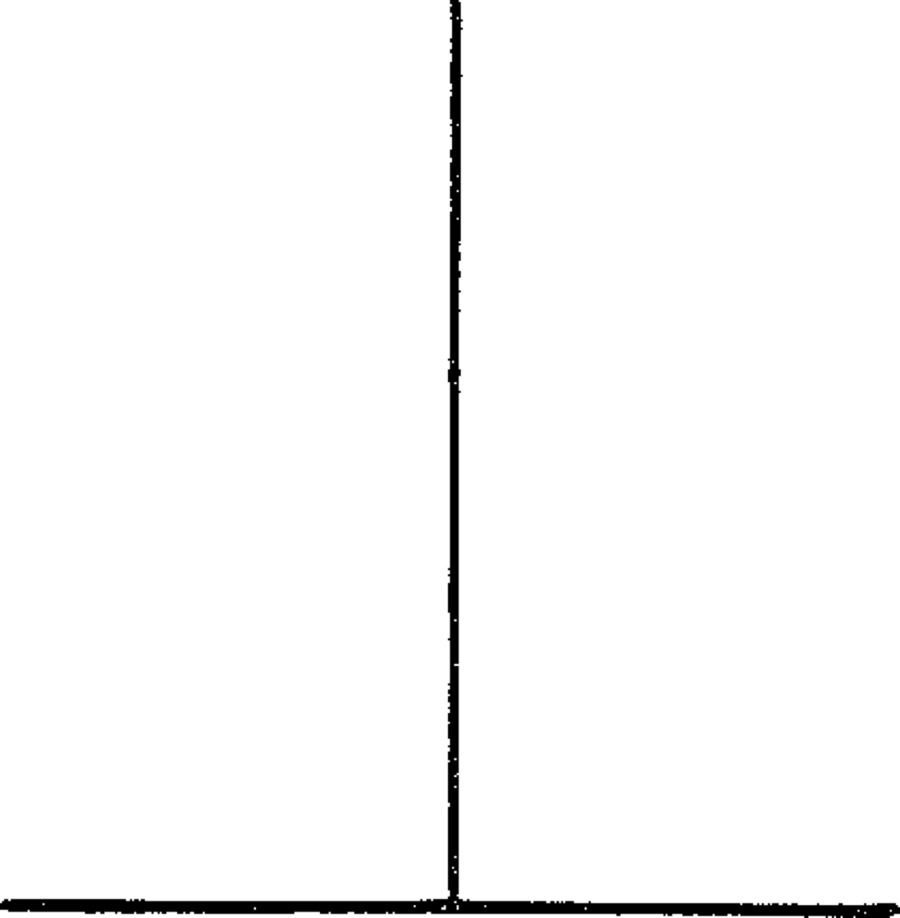
\includegraphics[width=4in]{img/illusions} \par}
	\caption{The sentence for \sysname{Illusions}.}
	\label{illusions}
\end{figure}

\sysname{IIlusions} has Properties 1, 3--5, and 7--8. Purely to clarify this fact, the 
following sequence of integers is presented as a model of the order in which 
associated ratios might appear in reality. (The sequence is otherwise totally 
inadequate as a model of \sysname{Illusions.}) $4 2 1$; $4 2$; $5 4 2 1$; $4 3 1$. The 
implication structure would then be as shown in figure \ref{illusionstructure}.

\begin{figure}
	{\centering 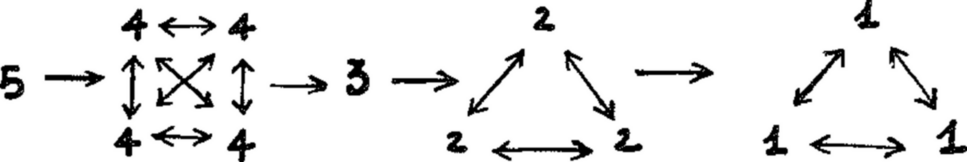
\includegraphics[width=4.5in]{img/illusionstructure} \par}
	\caption{Example implication structure for \sysname{Illusions}.}
	\label{illusionstructure}
\end{figure}

The axiom would be 4, and 5 could not appear in a proof. \sysname{IIlusions} has 
Property 1 on the basis that one can control the associated ratio. Turning to 
Property 4, it is normally the case that when an implication is repeated, a 
given occurrence of one of the sentences involved is unique to a specific 
occurrence of the implication. In \sysname{Illusions,} however, if two equal 
sentences are next smaller than X, the occurrence of X does not uniquely 
belong to either of the two occurrences of the implication. Compare figure \ref{thestructure},
where the occurrence of `$t$' is not unique to either occurrence of `$the$'. 
Subject to this explanation, \sysname{Illusions} has Property 4. \sysname{Illusions} has 
Property 8, but it goes without saying that the type of implication is not 
modus ponens. Properties 3, 5, and 7 need no comment. As for Property 2, 
the rule of implication refers to a property of sentences, rather than to 
elements of sentences. The interesting feature of \sysname{Illusions} is that it 
reverses the situation defined by Properties 6 and 9. Compound indirect 
implication is about the same as simple implication. The only difference is 
the difference between being smaller and being next smaller. And there is 
only one axiom (per person). 

\begin{figure}
	{\centering \begin{tabular}{c c c} t & h & e \\ h &   &   \\ e &   & \end{tabular} \par}
	\caption{Structure with shared node.}
	\label{thestructure}
\end{figure}


Simple direct implication, however, is subjective and illusive. It 
essentially involves changing one's perceptions of an illusion. The change of 
associated ratios is subjective, elusive, and certainly not numerically 
measurable. Then, the order in which one sees sentences won't always be 
their order in the implications and proofs. And even though one is exposed 
to all the sentences, one may have difficulty distinguishing and remembering 
them in consciousness. If I see the normal illusion, then manage to get 
myself to see the lines as being of equal length, I know I have seen a 
theorem. What is difficult is grasping the steps in between, the simple direct 
implications. If the brain contains a permanent impression of every sensation 
it has received, then the implications objectively exist; but they may not be 
thinkable without neurological techniques for getting at the impressions. In 
any case, \enquote{proof} is well-defined in some sense---but proofs may not be 
thinkable. \sysname{Illusions} is, after all, not so much shakier in this respect than 
even simple arithmetic, which contains undecidable sentences and 
indefinable terms. 

In \booktitle{The Logical Syntax of Language}, Carnap distinguishes pure syntax 
and descriptive syntax; and says that pure syntax should be independent of 
notation, and that every system should be isomorphic to some ink-on-paper 
system. In so doing, Carnap violates his own \uline{Principle of Tolerance}. Consider 
the following trivial formalist system. 

\midheading{\enquote{Order}}

\begin{sysrules}
A \enquote{sentence} is a member of a finite set of integers. 

Sentence Y is \enquote{implied by} sentence X if and only if Y=X, or else of all the 
sentences, Y is the one next smaller than X. 

Take as the axiom the largest sentence. 
\end{sysrules}

Is the pure syntax of \sysname{Illusions} isomorphic to \sysname{Order}? The preceding 
paragraph proved that it is not. The implication structure of \sysname{Order} is 
mechanical to the point of idiocy, while the implication structure of 
\sysname{Illusions} is, as I pointed out, elusive. Figure \ref{orderstruc}
where loops indicate multiple occurances of the same sentence, could 
adequately represent a proof in \enquote{Order,} but could not remotely represent 
one in \sysname{Illusions.} The essence of \sysname{Illusions} is that it is coupled to the 
reader's subjectivity. For an ink-on-paper system even to be comparable to 
\sysname{IIlusions,} the subjectivity would have to be moved out of the reader and 
onto the paper. This is utterly impossible. 

\begin{figure}
	{\centering 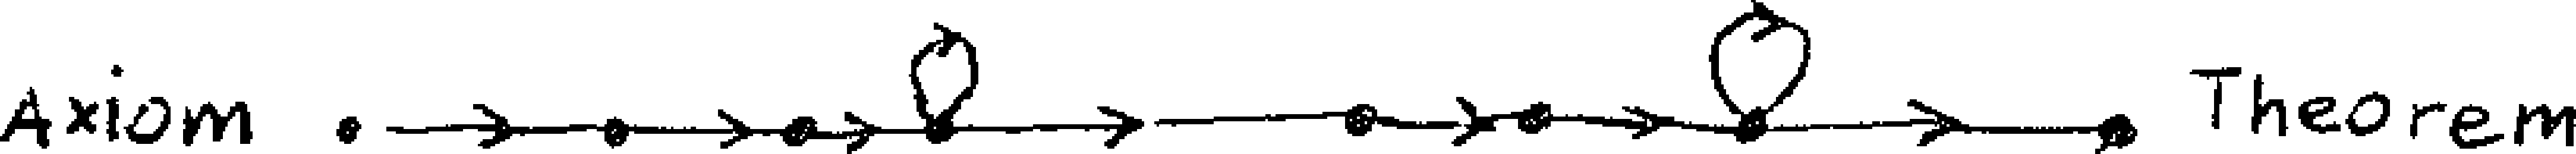
\includegraphics[width=4.5in]{img/orderstructure} \par}
	\caption{Implication structure of \sysname{Order}.}
	\label{orderstruc}
\end{figure}

Here is the next system. 

\midheading{\sysname{Innperseqs}}

\begin{sysrules}
Explanation: Consider the rainbow halo which appears to surround a small 
bright light when one looks at it through fogged glass (such as 
eyeglasses which have been breathed on). The halo consists of 
concentric circular bands of color. As the fog evaporates, the halo 
uniformly contracts toward the light. The halo has a vague outer 
ring, which contracts as the halo does. Of concern here is what 
happens on one contracting radius of the halo, and specifically 
what happens on the segment of that radius lying in the vague 
outer ring: the outer segment. 

A \enquote{sentence} (or halopoint) is the changing halo color at a fixed point, in 
space, in the halo; until the halo contracts past the point. 

Several sentences \enquote{imply} another sentence if and only if, at some instant, 
the several sentences are on an outer segment, and the other 
sentence is the inner endpoint of that outer segment. 

An \enquote{axiom} is a sentence which is in the initial vague outer ring (before it 
contracts), and which is not an inner endpoint. 

An \enquote{innperseq} is a sequence of sequences of sentences on one radius 
satisfying the following conditions. 1. The members of the first 
sequence are axioms, 2. For each of the other sequences, the first 
member is implied by the non-first members of the preceding 
sequence; and the remaining inembers (if any) are axioms or first 
members of preceding sequences. 3. All first members, of 
sequences other than the last two, appear as non-first members. 4. 
No sentence appears as a non-first member more than once. 5. The 
last sequence has one member. 
\end{sysrules}


{\centering
\begin{minipage}{1.6in}\imgw{1.3in}{img/innperseqs}\end{minipage}
	\begin{minipage}{2.25in}
\enquote{Sentences} at 

	\begin{tabular}{ c r l }
		\bimg{time1} & $time_1$: & $a_1 a_2 a_3 a_4 a_5 a_6 a_7 b$ \\
		& & $a_1,a_2 \rightarrow\ b$ \\
	\end{tabular}

	\begin{tabular}{c r l}
		\bimg{time2} & $time_2$: & $a_2 a_3 a_4 a_5 a_6 a_7 b c$ \\
		& & $a_3 \rightarrow\ c$ \\
	\end{tabular}

	\begin{tabular}{c r l}
		\bimg{time3} & $time_3$: & $a_4 a_5 a_6 a_7 b c d$ \\
		& & $a_4,a_5 \rightarrow\ d$ \\
	\end{tabular}

	\begin{tabular}{c r l}
		\bimg{time4} & $time_4$: & $a_6 a_7 b c d e$ \\
		& & $a_6,b \rightarrow\ e$ \\
	\end{tabular}

	\begin{tabular}{c r l}
		\bimg{time5} & $time_5$: & $a_7 b c d e f$ \\
		& & $a_7,c \rightarrow\ f$ \\
	\end{tabular}

	\begin{tabular}{c r l}
		\bimg{time6} & $time_6$: & $c d e f g$ \\
		& & $d,e \rightarrow\ g$ \\
	\end{tabular}

\enquote{Axioms} $a_1 a_2 a_3 a_4 a_5 a_6 a_7$


Innperseq \\
$(a_3,a_2,a_1)$
$(b,a_3)$
$(c,a_5,a_4)$
$(d,b,a_6)$
$(e,c,a_7)$
$(f,e,d)$
$(g)$
	\end{minipage}\par}

In the diagram, different positions of the vague outer 
ring at different times are suggested by different shadings. The 
outer segment moves \enquote{down the page.} The figure is by no means 
an innperseq, but is supposed to help explain the definition. 
In \sysname{Innperseqs,} a conventional proof would be redundant unless all 
the statements were on the same radius. And even if the weakest axiom were 
chosen (the initial outer endpoint), this axiom would imply the initial inner 
endpoint, and from there the theorem could be reached immediately. In 
other words, to use the standard definition of \enquote{proof} in \sysname{Innperseqs} 
would result in an uninteresting derivation structure. Thus, a more 
interesting derivation structure is defined, the \enquote{\term{innperseq.}} The interest of 
an \enquote{\term{innperseq}} is to be as elaborate as the many restrictions in its definition 
will allow. Proofs are either disregarded in \sysname{Innperseqs}; or else they are 
identified with innperseqs, and lack Property 8. \sysname{Innperseqs} makes the 
break with the proof-theorem structure of formalist mathematics. 

Turning to simple implication, an implicand can have many impliors; 
and there is an infinity of axioms, specified by a general condition. The 
system has Property 1 in the sense that a sentence can exist at different 
times and be a member of different implications. It has Property 4 in the 
sense that the sentences in a specific implication can exist at different times, 
and the implication holds as long as the sentences exist. It has Property 3 in 
that an inner endpoint implies itself. The system also has Properties 5 and 7; 
and lacks Property 2. But, as before, Properties 6 and 9 are another matter. 
Given several sentences, it is certainly possible to tell mechanically whether 
one is implied by the others. But when are you given sentences? If one can 
think the sentences, then relating them is easy---but it is difficult to think the 
sentences in the first place, even though they objectively exist. The diagram 
suggests what to look for, but the actual thinking, the actual sentences are 
another matter. As for Property 9, when \enquote{theorems} are identified with last 
members of innperseqs, I hesitate to say whether a derivation of a given 
sentence can be constructed mechanically. If a sentence is nearer the center 
than the axioms are, an innperseq can be constructed for it. Or can it? The 
answer is contingent. \enquote{Innperseqs} is indeterminate because of the difficulty 
of thinking the sentences, a difficulty which is defined into the system. It is 
the mathematician's capabilities at a particular instant which delimit the 
indeterminacies. Precisely because of the difficulty of thinking sentences, I 
will give several subvariants of the system. 

\midheading{Indeterminacy}

\begin{sysrules}
A \enquote{totally determinate innperseq} is an innperseq in which one thinks all the 
sentences. 

An \enquote{implior-indeterminate innperseq} is an innperseq in which one thinks 
only each implicand and the outer segment it terminates. 

A \enquote{sententially indeterminate innperseq} is an innperseq in which one thinks 
only the outer segment, and its inner endpoint, as it progresses 
inward. 
\end{sysrules}


Let us return to the matter of pure and descriptive syntax. The interest 
of \enquote{Illusions} and \enquote{Innperseqs} is precisely that their abstract structure 
cannot be separated from their physical and psychological character, and 
thus that they are not isomorphic to any conventional ink-on-paper system. I 
am trying to break through to unheard of, and hopefully significant, modes 
of implication; to define implication structures (and derivation structures) 
beyond the reach of past mathematics. 

\subsection{Constructed Memory Systems}

In order to understand this section, it is necessary to be thoroughly 
familiar with \essaytitle{Studies in Constructed Memories,} the essay following this 
one. (I have not combined the two essays because their approaches are too 
different.) I will define post-formalist systems in constructed memories, 
beginning with a system in an M*-Memory. 

\midheading{\enquote{Dream Amalgams}}

\begin{sysrules}
A \enquote{sentence} is a possible method, an $A_{a_i}$. with respect to an M*-Memory. 
The sentence $A_{a_p}$ \enquote{implies} the sentence $A_{a_q}$ if and only if the $a_q$th 
M*-assertion is actually thought; and either $A_{a_q} = A_{a_p}$, or else there is 
cross-method contact of a mental state in $A_{a_q}$ with a state in $A_{q_p}$\footnote{sic?}

The axioms must be chosen from sentences which satisfy two conditions. 
The mental states in the sentences must have cross-method contact 
with mental states in other sentences. And the M*-assertions 
corresponding to the sentences must not be thought. 

Explanation: As \essaytitle{Studies in Constructed Memories} says, there can be 
cross-method contact of states, because a normal dream can 
combine totally different episodes in the dreamer's life into an 
amalgam. 
\end{sysrules}

\enquote{\textsc{Dream Amalgams}} has Properties 1--5. For the first time, sentences are 
structurally composite, with mental states being the relevant sentential 
elements. Implication has an unusual character. The traditional type of 
implication, modus ponens, is \enquote{directed,} because the conditional is 
directed. Even if $\ulcorner\varphi\supset\phi\urcorner$ is true 
$\ulcorner\varphi\supset\phi\urcorner$ may not be. Now implication is also 
directed in \enquote{\textsc{Dream Amalgams,}} but for a very different reason. 
Cross-method contact, unlike the conditional, has a symmetric character. 
What prevents implication from being necessarily symmetrical is that the 
implicand's M*-assertion actually has to be thought, while the implior's 
M*-assertion does not. Thus, implication is both subjective and mechanical, 
it is subjective, in that it is a matter of volition which method is remembered 
to have actually: been used. It is mechanical, in that when one is 
remembering, one is automatically aware of the cross-method contacts of 
states in $A_{a_q}$. The conditions on the axioms ensure that they will have 
implications without losing Property 7. 

As for compound implication in \enquote{\textsc{Dream Amalgams,}} the organism 
with the M*-Memory can't be aware of it at all; because it can't be aware 
that at different times it remembered different methods to be the one 
actually used. (In fact, the organism cannot be aware that the system has 
Property 5, for the same reason.) On the other hand, to an outside observer 
of the M*-Memory, indirect implication is not only thinkable but 
mechanical. It is not superfluous because cross-method contact of mental 
states is not necessarily transitive. The outside observer can decide whether a 
sentence is a theorem by the following mechanical procedure. Check 
whether the sentence's M*-assertion has acually been thought; if so, check all 
sentences which imply it to see if any are axioms; if not, check all the 
sentences which imply the sentences which imply it to see if any are axioms; 
etc. The number of possible methods is given as finite, so the procedure is 
certain to terminate. Again, an unprecedented mode of implication has been 
defined. 

When a post-formalist system is defined in a constructed memory, the 
discussion and analysis of the system become a consequence of constructed 
memory theory and an extension of it. Constructed memory theory, which 
is quite unusual but still more or less employs deductive inference, is used to 
study post-formalist modes of inference which are anything but deductive. 

To aid in understanding the next system, which involves infalls in a 
D-Memory, here is an 

{ \vskip 1.5em \centering \large \framebox[1.1\width]{\enquote{Exercise to be Read Aloud}} \par\vskip 1.5em}

(Read according to a timer, reading the first word at O' O", and prolonging 
and spacing words so that each sentence ends at the time in parentheses after 
it. Do not pause netween sentences.) 

\begin{tabular}{ r p{2.5in} }
	($event_1$) &  All men are mortal. (17") \\

	($Sentence_1=event_2s$) &  The first utterance lasted 17" and ended at 17"; and lasted 15" and ended 1" ago. (59") \\

	($S_2=event_3$) & The second utterance lasted 42" and ended at 59": and lasted 50" and ended 2" ago. (1' 31") \\

	($S_3=event_4$) & The third utterance lasted 32" and ended at 1' 31"; and lasted 40" and ended 1" ago. (2' 16") \\
\end{tabular}

Since '32' in $S_3$ is greater than '2' in $S_2$, $S_2$ must say that $S_1$ ($=event_2$)
ended 30" after $S_2$ began, or something equally unclear. The duration of $S_2$
is greater than the distance into the past to which it refers. This situation is 
not a real infall, but it should give the reader some intuitive notion of an 
infall. 

\midheading{"Infalls"}

\begin{sysrules}
	A "sentence" is a D-sentence, in a D-Memory such that $event_{j+1}$ is the first 
thinking of the jth D-sentence, for all j. 

Two sentences "imply" another if and only if all three are the same; or else 
the three are adjacent (and can be written $S_{j+1},S_j,S_{j-1}$), and are such 
that $\delta_j=x_{j+1}-x_j> z_j,$ $S^D_{j-1}$ is the implicand. (The function of $S_{j+1}$ is to 
give the duration $\delta_j=x_{j+1}-x_j$ of $S_j$. $S_j$ states that $event_j$, the first 
thinking of $S^{D}_{j-1}$, ended at a distance $z_j$ into the past, where $z_j$ is smaller 
than $S^D_j$'s own duration. The diagram indicates the relations.) 
\end{sysrules}

\imgw{4in}{img/infallsdiag}

In this variety of D-Memory, the organism continuously thinks successive 
D-sentences, which are all different, just as the reader of the above exercise 
continuously reads successive and different sentences. Thus, the possibility 
of repeating a sentence depends on the possibility of thinking it while one is 
thinking another sentence---a possibility which may be far-fetched, but which 
is not explicitly excluded by the definition of a "D-Memory." If the 
possibility is granted, then "\textsc{Infalls}" has Properties 1--5. Direct implication is 
completely mechanical; it is subjective only in that the involuntary 
determination of the $z_j$ and other aspects of the memory is a 'subjective' 
process of the organism. Compound implication is also mechanical to an 
outside observer of the memory, but if the organism itself is to be aware of 
it, it has to perform fantastic feats of multiple thinking. 

"\textsc{Dream Amalgams}" and "\textsc{Infalls}" are systems constructed with 
imaginary elements, systems whose "notation" is drawn from an imaginary 
object or system. Such systems have no descriptive syntax. Imaginary objects 
were introduced into mathematics, or at least into geometry, by Nicholas 
Lobachevski, and now I am using them as a notation. For these systems to 
be nonisomorphic to any ink-on-paper systems, the mathematician must be 
the organism with the M*-Memory or the D*-Memory. But this means that 
in this case, the mathematics which is nonisomorphic to any ink-on-paper 
system can be performed only in an imaginary mind. 

Now for a different approach. Carnap said that we are free to choose 
the rules of a system arbitrarily. Let us take Carnap literally. I want to 
construct more systems in constructed memories---so why not construct the 
system by a procedure which ensures that constructed memories are 
involved, but which is otherwise arbitrary? Why not suspend the striving 
after "interesting" systems, that last vestige of the striving after 
"correctness," and see what happens? Why not construct the rules of a 
system by a chance procedure? 

To construct a system, we have to fill in the blanks in the following rule 
schema in such a way that grammatically correct sentences result. 

\newcommand{\blankspace}{\_\_\_\_\_\_\_\_\_\_}

\midheading{Rule Schema}

\begin{sysrules}
A "sentence" is a(n) \blankspace.

Two sentences "imply" a third if and only if the two sentences \blankspace\ the third. 

An "axiom" is a sentence that \blankspace.
\end{sysrules}


I now spread the pages of \essaytitle{Studies in Constructed Memories} on the floor. 
With eyes closed, I hold a penny over them and drop it. I open my eyes and 
copy down the expressions the penny covers. By repeating this routine, I 
obtain a haphazard series of expressions concerning constructed memories. It 
is with this series that I will fill in the blanks in the rule schema. In the next 
stage, I fill the first (second, third) blank with the ceries of expressions 
preceding the-first (second, third) period in the entire series. 

\midheading{"Haphazard System"}

\begin{sysrules}
A "sentence" is a the duration D-sentences $\triangle\ (\mathparagraph^m)$ conclude these 
"$\Phi^*$-Reflec\-tion," or the future Assumption voluntarily force of 
conviction for conclusion the Situation or by ongoing that this 
system? be given telling between the Situation 1. 

Two sentences "imply" a third if and only if the two sentences is\slash was 
contained not have to the acceptance that a certain and malleable 
study what an event involves material specifically mathematics: 
construct accompanies the rest, extra-linguistically image organism 
can fantasy not remembering $\Phi^*$-Memory, the future interval defined 
in dream the third. 

An "axiom" is a sentence that internally D-sentences, just as the 
"$\Phi^*$-Memory" sentences $A_{a_1}$ is $A_{a_2}$. 

In the final stage, I cancel the smallest number of words I have to in 
order to make the rules grammatical. 
\end{sysrules}

\midheading{"Fantasied Amnesia"}

\begin{sysrules}
A "sentence" is a duration or the future force of conviction for the Situation 
or this system given Situation 1. 

Two sentences "imply" a third if and only if the two sentences have the 
acceptance that a certain and malleable study extra-linguistically can 
fantasy not remembering the future interval defined in the third. 

An "axiom" is a sentence that internally just sentences $A_{a_2}$.
\end{sysrules}

It becomes clear in thinking about "Fantasied Amnesia" that its 
metametamathematics is dual. Describing the construction of the rules, the 
metamathematics, by a systematic performance, is one thing. Taking the 
finished metamathematics at face value, independently of its origin, and 
studying it in the usual manner, is another. Let us take "Fantasied Amnesia" 
at face value. As one becomes used to its rules, they become somewhat more 
meaningful. I will say that an "interpretation" of a haphazard system is an 
explanation of its rules that makes some sense out of what may seem 
senseless. "Interpreting" is somewhat like finding the conditions for the 
existence of a constructed memory which seemingly cannot exist. The first 
rule of "Fantasied Amnesia" is a disjunction of three substantives. The 
"Situation" referred to in the second substantive expression is either 
Situation 1 or else an unspecified situation. The third substantive expression 
apparently means "this system, assuming Situation 1," and refers to 
"Fantasied Amnesia" itself. The definition of "sentence" is thus meaningful, 
but very bizarre. The second rule speaks of "the acceptance" as if it were a 
written assent. The rule then speaks of a "malleable study" as "fantasying" 
something. This construction is quite weird, but let us try to accept it. The 
third rule speaks of a sentence that "sentences" (in the legal sense) a possible 
method. So much for the meaning of the rules. 

Turning to the nine properties of formalist systems, the reference to 
"the future interval" in the implication rule of "Fantasied Amnesia" 
indicates that the system has Property 2; and the system can perfectly well 
have Property 8. It does not have Property 6 in any known sense. Certainly 
it does have Property 9. it just might have Property. 1. But as for the other 
four properties, it seems out of the question to decide whether "Fantasied 
Amnesia" has them. For whatever it is worth, "Fantasied Amnesia" is on 
balance incomparable to formalist systems. 

My transformation rule schema has the form of a biconditional, in 
which the right clause is the operative one. If a transformation rule were to 
vary, in such a way that it could be replaced by a constant rule whose right 
clause was the disjunction of the various right clauses for the variable rule, 
then the latter would vary "trivially." 1 will say that a system whose 
transformation rule can vary non-trivially is a "heterodeterminate" system. 
Since 1 have constructed a haphazard metamathematics, why not a 
heterodeterminate metamathematics? Consider a mathematician with an 
M-Memory, such that each $A_{a_i}$. is the consistent use of a different 
transformation rule, a different definition of "imply," for the mathematics 
in which the mathematician is discovering theorems. The consistent use of a 
transformation rule is after all a method---a method for finding the 
commitments premisses make, and for basing conclusions in premisses. When 
the mathematician goes to remember which rule of inference he has actually 
been using, he "chooses" which of the possible methods is remembered to 
have actually been used. This situation amounts to a heterodeterminate 
system. tn fact, the metamathematics cannot even be written out this time; I 
can only describe it metametamathematically in terms of an imaginary 
memory. 

We are now in the realm of mathematical systems which cannot be 
written out, but can only be described metametamathematically. I will 
present a final system of this sort. It is entitled \textsc{"System Such That No One 
Knows What's Going On."} One just has to guess whether this system exists, 
and if it does what it is like. The preceding remark is the 
metametamathematical description, or definition, of the system. 

\subsection{Epilogue}

Ever since Carnap's Principle of Tolerance opened the floodgates to 
arbitrariness in mathematics, we have been faced with the prospect of a 
mathematics which is  indistinguishable from  art-for-art's-sake, or 
amusement-for-amusement's-sake. But there is one characteristic which saves 
mathematics from this fate. Mathematics originated by abstraction from 
primitive technology, and is indispensable to science and technology---in 
short, mathematics has scientific applications. The experience of group 
theory has proved, I hope once and for all, the bankruptcy of that narrow 
practicality which would limit mathematics to what can currently be applied 
in science. But now that mathematics is wide open, and anything goes, we 
should be aware more than ever that scientific applicability is the only 
objective value that mathematics has. I would not have set down constructed 
memory theory and the post-formalist systems if I did not believe that they 
could be applied. When and how they will be is another matter. 

And what about the "validity" of formalism? The rise of the formalist 
position is certainly understandable. The formalists had a commendable, 
rationalistic desire to eliminate the metaphysical problems associated with 
mathematics. Moreover, formalism helped stimulate the development of the 
logic needed in computer technology (and also to stimulate this paper). In 
spite of the productiveness of the formalist position, however, it now seems 
beyond dispute that formalism has failed to achieve its original goals. (My 
pure philosophical writings are the last word on this issue.) Perhaps the main 
lesson to be learned from the history of formalism is that an idea does not 
have to be "true" to be productive. 


\section*{Note}
Early versions of \textsc{"Illusions"} and \textsc{"Innperseqs"} appeared in my essay 
"Concept Art," published in An Anthology, ed. La Monte Young, New 
York, 1963. An early, July 1961 version of \textsc{"System Such That No One 
Knows What's Going On"} appeared in dimension 14, Ann Arbor, 1963, 
published by the University of Michigan College of Architecture and Design. 


\chapter{Studies in Constructed Memories}

\section{Introduction}

The memory of a conscious organism is a phenomenon in which 
interrelations of mind, language, and the rest of reality are especially evident. 
In these studies, I will define some conscious memory-systems, and 
investigate them. The investigation will be mathematical. In fact, the nearest 
precedent for it is perhaps the geometry of Nicholas Lobachevski. 
Non-Euclidian geometry had many founders, but Lobachevski in particular 
spoke of his system as an "imaginary geometry." Lobachevski's system was, 
so to speak, the physical geometry of an "imaginary," or constructed, space. 
By analogy, my investigation could be called a psychological algebra of 
constructed minds. It is too early to characterize the investigation more 
exactly. Let us just remember Rudoiph Carnap's Principle of Tolerance in 
mathematics: the mathematician is free to construct his system in any way 
he chooses. 

I will begin by introducing a repertory of concepts informally, 
becoming more formal as I go along. Consider ongoing actions, which by 
definition extend through past, present, and future. For example, "I am 
making the trip from New York to Chicago." Consider also past actions 
which have probable consequences in the present. "I have been heating this 
water" (entailing that it isn't frozen now). I will be concerned with such 
actions as these. 

Our language provides for the following assertion: "I am off to the 
country today; I could have been off to the beach; I could not possibly have 
been going to the center of the sun". We distinguish an actual action from a 
possible action; and distinguish both from an action which is materially 
impossible. People insist that there are things they could do, even though 
they don't choose to do them (as opposed to things they couldn't do). What 
distinguishes these possible actions from impossible ones? Rather than 
trying to analyze such everyday notions in terms of the logic of 
counterfactual conditionals, or of modalities, or of probability, I choose to 
take the notions at their face value. My concern is not to philosophize, but 
to assemble concepts with which to define an interesting memory system. 

What is the introspective psychological difference between a thought 
that has the force of a memory, and a thought that has the force of a 
fantasied past, a merely possible past? I am not asking how I know that a 
verbalized memory is true; I am asking what quality a naive thought has that 
marks it as a memory. Let Alternative E be that I went to an East Side 
restaurant yesterday, and Alternative W be that I went to a West Side one. 
By the "thought of E" I mean mainly the visualization of going into the East 
Side restaurant. My thought of E has the force of memory. It actually 
happened. W is something I could have done. I can imagine I did do W. There 
is nothing present which indicates whether I did E or W. Yet W merely has 
the force of possibility, of fantasy. How do the two thoughts differ? Is the 
thought of E involuntarily more vivid? Is there perhaps an "attitude of 
assertion" involuntarily present in the thought of E? 

Consider the memory that I was almost run down by a truck yesterday: 
I could have been run down, but wasn't. In such a case, the possibility that I 
could have been run down would be more vivid than the actuality that I 
wasn't. (Is it not insanity, when a person is overwhelmed by the fear of a 
merely possible past event? ) My hold on sanity here would be the awareness 
that I am alive and well today. 

In dreams, do we not wholeheartedly "remember" that a misfortune 
has befallen us, and begin to adjust emotionally to it? Then we awake, and 
wholeheartedly remember that the misfortune has not befallen us. The 
thought that had the force of memory in the dream ceases to have that force 
as we awake. We remember the dream, and conclude that it was a fantasy. 
Even more characteristic of dreams, do I not to all intents and purposes go 
to far places and carry out all sorts of actions in a dream, only to awaken in 
bed? We say that the dream falsifies my present environment, my 
sensations, my actions, memories, the past, my whole world, in a totally 
convincing way. Can a hypnotist produce artificial dreams, that is, can he 
control their content? Can the hypnotist give his subject one false memory 
one moment, and replace it with a contradictory memory the next 
moment? 

I will now specify a situation involving possible actions and 
remembering. 

Situation 1. "I could have been accomplishing G by doing $A_{a_1}$, or by 
doing $A_{a_2}$, \ldots, or by doing $A_{a_n}$; but I have actually been accomplishing G by 
doing $A_{a_1}$." Here the ongoing actions $A_{a_i}$, $i=1,...,n$,$a_i\neq a_h if i\neq h$, are 
the possible methods of accomplishing G. (The subscripts are supposed to 
indicate that the methods are distinct and countable, but not ordered.) The 
possible methods cannot be combined, let us assume. 

In such a situation, perhaps the thought that I have been doing $A_{a_1}$
would be distinguished from similar thoughts about $A_{a_2}, ..., A_{a_n}$ by the
presence of the "attitude of assertion". Since the possible methods are 
ongoing actions, the thought that I have been doing $A_{a_i}$ has logical or 
probabie consequences I can check against the present. 

Now $A_{a_1}$, is actual and $A_{a_2}$ is not, so that $A_{a_1}$, simply cannot have 
possible jar in $A_{a_3}$ to contain it. The only "connection" $A_{a_1}$ could have
material contact with $A_{a_2}$. An actual liquid in $A_{a_1}$ could not require a 
with $A_{a_2}$, would be verbal and gratuitous. Therefore, in order to be possible 
methods, $A_{a_2}$, ..., $A_{a_n}$ must be materially separable. A liquid in $A_{a_2}$ must
not require a jar in $A_{a_3}$ to contain it. If it did, $A_{a_2}$ couldn't be actualized 
while $A_{a_3}$, remained only a possibility. 

Enough concepts are now at hand for the studies to begin in earnest. 

\section{M-Memories}

\newcommand{\definition}{\textbf{Definition.}}
\newcommand{\assumption}[1]{\textit{Assumption #1.}}
\newcommand{\conclusion}[1]{\textbf{Conclusion #1.}}

\definition Given the sentences "I have actually been doing $A_{a_i}$", where 
the $A_{a_i}$ are non-combinable possible methods as in Situation 1, an 
"M-Memory" is a memory of a conscious organism such that the organism 
can think precisely one of the sentences at a time, and any of the sentences 
has the force of memory. 

This definition refers to language, mind, and the rest of reality in their 
interrelations, but the crucial reference is to a property of certain sentences. 
I have chosen this formulation precisely because of what I want to 
investigate. I want to find the minimal, elegant, extra-linguistic conditions, 
whatever they may be, for the existence of an M-Memory (which is defined 
by a linguistic property). I can say at once that the conditions must enable 
the organism to think the sentences at will, and they must provide that the 
memory is consistent with the organism's present awareness. 

\definition The "P-Memory" of a conscious organism is its conscious 
memory of what it did and what happened to it, the past events of its life. I 
want to distinguish here the "personal" memory from the preconscious. 

\definition An "L-Memory" is a linguistic P-Memory having no 
extra-linguistic component. Of course, the linguistic component has 
extra-linguistic mental associations which give it "meaning"--otherwise the 
memory wouldn't be conscious. But these associations lack the force of a 
mental reliving of the past independent of language. An L-Memory amounts 
to extra-linguistic amnesia. 

\assumption{1.1} With respect to normal human memory, when I forget 
whether I did x, I can't voluntarily give either the thought that I did x, or 
the thought that I didn't do x, the force of memory. I know that I either did 
or didn't do x, but I can create no conviction for either alternative. (An 
introspective observation.) 

\conclusion{1.2} An L-Memory is not sufficient for an M-Memory, even 
in the trivial case that the $A_{a_i}$ are beyond perception (as internal bodily 
processes are). True, there would be no present perceptions to check the 
sentences "I have actually been doing $A_{a_i}$" against. True, the L-Memory 
precludes any extra-linguistic memory-"feelings" which would conflict with 
the sentences. But the L-Memory is otherwise normal. And \textit{Assumption 1.1}
indicates that normally, either precisely one of a number of mutually 
exclusive possibilities has the force of memory; or else the organism can give 
none of them the force of memory. 

\assumption{1.3} I cannot, from within a natural dream, choose to swith 
to another dream. (An introspective observation. A "natural" dream is a 
dream involuntarily produced internally during sleep.) 

\conclusion{1.4} An M-Memory could not be produced by natural 
dreaming. It is true that in one dream one sentence could have the force of 
memory, and in another dream a different sentence could. But an M-Memory 
is such that the organism can choose one sentence-memory one moment and 
another the next. See Assumption 1.3. 

\assumption{1.5} Returning to the example of the restaurants, I find 
that months after the event, my thought of E no longer has the force of 
memory. All I remember now is that I used to remember that I did E. I 
remember that I did E indirectly, by remembering that I remembered that I 
did E. (My memory that I did E is becoming an L-Memory.) The assumption 
is that a memory of one's remembering can indicate, if not imply, that the 
event originally remembered occurred. 

\conclusion{1.6} The following are adequate conditions for the existence 
of an M-Memory. 
\begin{enumerate}
\item The sentences are the organism's only memory of which 
method he has been using. 

\item When the organism thinks "I have actually been doing $A_{a_i}$".
then (he artificially dreams that) he has been doing $A_{a_i}$ --- and is 
now doing it. 

\item When the dream ends, he does not remember that he 
remembered that "he has been doing $A_{a_i}$," That is, he does not remember 
the dream; and he does not remember that he thought the sentence. These 
conditions would permit the existence of an M-Memory or else a memory 
indistinguishable to all intents and purposes from an M-Memory. 
\end{enumerate}

What I have in mind in \conclusion{1.6} is dreams which are produced 
artificially but otherwise have all the remarkable qualities of natural dreams. 
There would have to be a state of affairs such that the sentence would 
instantly start the dream going. 

So much for the conditions for the existence of an M-Memory. 
Consider now what it is like as a mental experience to have an M-Memory. 
What present or ongoing awareness accompanies an M-Memory? 
\conclusion{1.6.2} already told what the remembering is like. For the rest, I will 
informally sketch some conclusions. The organism can extra-linguistically 
image the $A_{a_i}$. The organism can think "I could have been doing $A_{a_i}$." When 
not remembering, the organism doesn't have to do any $A_{a_i}$, or he can do any 
one of them. The organism must not do anything which would liquidate a 
possble method, render the action no longer possible for him. 

\assumption{2.1} A normal dream can combine two totally different 
past episodes in my life into a fused episode, or amalgam; so that I "relive" it 
without doubts as.a single episode, and yet remain vaguely aware that 
different episodes are present in it. Dreams have the capacity not only to 
falsify my world, but to make the impossible believable. (An introspective 
observation.) 

\conclusion{2.2} The conditions for the existence of an M-Memory 
further permit material contact between the possible methods, the very 
contact which is out of the question in a normal Situation 1. The dream is so 
flexible that the organism can dream that an (actual) liquid is\slash was contained 
by a jar in a possible method. See \assumption{2.1} Thus, the $A_{a_i}$ do not have 
to be separable to be possible methods. 

I will now introduce further concepts pertaining to the mind. 

\definition\ A "mental state" is a mental "stage" or "space" or "mood" 
in which visualizing, remembering, and all imaging can be carried on. 

Some human mental states are stupor, general anxiety, empathy with 
another person, dizziness, general euphoria, clearheadedness (the normal 
state in which work is performed), and dreaming. In all but the last state, 
some simple visualization routine could be carried out voluntarily. Even ina 
dream, I can have visualizations, although here I can't have them at will. The 
states are not defined by the imaging or activities carried on while in them, 
but are "spaces" in which such imaging or activities are carried on. 

By definition. 

\conclusion{3.2} An M-Memory has to occur within the time which the 
possible methods require, the time required to accomplich G. By definition. 

\definition An "M*-Memory" is an M-Memory satisfying these 
conditions. 
\begin{enumerate}
\item $A_{a_i}$, for the entire time it requires, involves the voluntary 
assuming of mental states. $i=1,...,n$.
\item The material contact between the 
possible methods, the cross-method contact, is specifically some sort of 
contact between states. 
\end{enumerate}

\conclusion{3.3} For an M*-Memory, to remember is to choose the 
mental state in which the remembering is required to occur (by the 
memory). After all, for any M-Memory, to remember is to choose all the 
$A_{a_i}$-required things you are doing while you remember. 

By now, the character of this investigation should be clearer. I seek to 
stretch our concepts, rather that to find the "true" ones. The investigation 
may appear similar to the old discipline of philosophical psychology, but its 
thrust is rather toward the modern axiomatic systems. The reasoning is 
loose, but not arbitrary. And the investigation will become increasingly 
mathematical. 


\section{D-Memories}

\definition\ A "D-Memory" is a memory such that measured past time 
appears in it only in the following sentences: "$Event_j$ occurred in the interval 
% TODO\<F11><F12> ? whats up with AF
of time which is $x_j-x_{j-1}$ long and ended at $x_j$ AF, and is Yj long and ended $z_j$
\ ago," where $x_j$, $y_j$ and $z_j$ are positive numbers of time units (such as hours) 
and '$AF$' means "after a fixed beginning time." $x_O=O;$ $x_j> x_{j-1}$; and at any 
one fixed time, the intervals $|z_j, z_j+y_j|$ nowhere overlap. $y_j+z_j\leq x_j$ For an
integer $m$, the $m$th sentence acquires the force of memory, is added to the 
memory, at the fixed time $x_m$. $j=1, ..., f(t)$, where the number of sentences 
$f(t)$ is written as a function of time $AF$. Then $f(t)=m$ when $x_m \leq t \less x_{m+1}$. 
The sentences have the force of memory involuntarily. The organism does 
not make them up at will. 

Let me explain what the D-Memory involves. $Event_j$ is assigned to an 
abnormal "interval," a dual interval defined in two unrelated ways. The 
intervals defined by the $y_j$ and $z_j$ are tied to the present instant rather than to 
a fixed time, and could be written $|N-z_j-y_j, N-z_j|$, where '$N$' means "the time 
of the present instant relative to the fixed beginning time." 

\newcommand{\proof}{\textit{Proof}}

\conclusion{4} The intervals $|N-z_j-y_j, N-z_j|$ nowhere overlap. 

\proof: By definition, the intervals $|z_j, z_j+y_j|$ nowhere overlap. If $j\neq k$,
$|z_j, z_j+y_j|\cap|z_k, z_k+y_k|=\emptyset$ 
This fact implies that \eg $z_j\less z_j+y_j\less z_k\less z_k+y_k$.
Then $N-z_k-y_k\less N-z_k\less N-z_j-y_j\less N-z_j$.
Then $|N-z_k-y_k, N-z_k|\cap|N-z_j-y_j, N-z_j|=\emptyset$
At any one time, the organism can think of all the sliding intervals, and they 
partly cover the time up to now without overlapping. 

Suppose you find the deck of n cards 

{ \centering
\framebox[1.1\width]{
	\centering
	$event_j$ \linebreak
	$z_j$ ago}}


($j=1,...,n$ and $z_j$ is a positive number of days), and you have no 
information to date them other than what they themselves say. If you 
believe the cards, your mental experience will be a little like having a 
D-Memory. Then, the definition does not require that $y_j=x_j-x_{j-1}$. Again, it is 
not that two concepts of "length" are involved, but that the "interval" is 
abnormal. Of course this is all inconsistent, but I want to study the 
conditions under which a mind will accept inconsistency. 

\assumption{5.1} With respect to normal human memory, it is possible 
to forget what day it is, even though one remembers a past date. (An 
empirical observation.) 

\assumption{5.2} This assumption is based on the fact that the sign 
'CLOSED FOR VACATION. BACK IN TWO WEEKS' was in the window of 
a nearby store for at least a month this summer; and the fact that a 
filmmaker wrote in a newspaper, "When an actor asks me when the film will 
be finished, I say 'In two months," and two months later I give the same 
answer, and I'm always right.' Even in normal circumstances, humans can 
maintain a dual and outright inconsistent awareness of measured time. [n 
general, inconsistency is a normal aspect of human thinking and even has 
practical value. 

Imagine a child who has been told to date events by saying, for 
example, x happened two days ago, and a day later saying again, x happened 
two days ago---and who has not been told that this is inconsistent. What 
conditions are required for the acceptance of this dating system? It is 
precisely because of Assumptions 5.1 and 5.2 that a certain answer cannot 
be given to this question. The human mind is so flexible and malleable that 
there is no telling how much inconsistency it can absorb. I can only study 
what flaws might lead the child to reject the system. The child might "feel" 
that an event recedes into the past, something the memory doesn't express. 
An event might be placed by the memory no later than another, and yet 
"feel" more recent than the other. I speculate that if anything will discredit 
the system, it will be its conflict with naive, "felt," extra-linguistic memory. 

\conclusion{5.3} The above dating system would be acceptable to an 
organism with an L-Memory. 

\conclusion{5.4} The existence of an L-Memory is an adequate condition 
for the existence of a D-Memory. With extra-linguistic amnesia, the 
structure of the language would be the structure of the past in any case. The 
past would have no form independent of language. Anyway, time is gone for 
good, leaving nothing that can be checked directly. Without an 
extra-linguistic memory to fall back on, and considering Assumptions 5.1 
and 5.2, the dual temporal memory shouldn't be too much to absorb. 

As I said, the real difficulty with this line of investigation is putting 
limits on anything so flexible as the mind's capacity to absorb inconsistency. 

Now the thinking of a sentence in a D-Memory itself takes time. Let 
$\delta(S^D_j)$ be the minimum number of time units it takes to think the jth 
D-sentence. This function, abbreviated '$\delta_j$', is the duration function of the 
D-sentences. 

\conclusion{6.1} If $\delta_j\greater z_j$, the memory of the interval defined by $y_j$ and 
$z_j$ places the end of the interval after the beginning of the memory of it, or 
does something else equally unclear. If $\delta_j\greater y_j+z_j$, the entire interval is placed 
after the beginning of the memory of it. When $\delta_j\greater z_j$, let us say that the end 
of the remembered interval falis within the interval for the memory of it, or 
that the situation is an "\textsc{infall}." (Compare \said{The light went out a half-second 
ago}.)

\conclusion{6.2} If $\delta_j\greater x_{j+k}-x_j$, then $S^D_{j+k}$ is added to the preconscious 
before $S^D_j$ can be thought once. The earliest interval during which the jth 
sentence can be thought "passes over" the (j+k)th interval. Let us say that 
the situation is a "\textsc{passover}." (Something of the sort is true of humans, 
whose brains contain permanent impressions of far more sensations than can 
be thought, remembered in consciousness.) 

\conclusion{6.3} If there are passovers in a D-Memory, the organism 
cannot both think the sentences during the earliest intervals possible and be 
aware of the passovers. 

\proof: The only way the organism can be aware of $\delta(S_j)$
is for $event_{j+h}$ (h a positive integer) to be the thinking of $S_j$. 
If the thinking of $S_j$ takes piace as the $(j+1)^{th}$ event, then the organism gets two 
values for $\delta(S_j)$, namely $x_{j+1}-x_j$ and $y_{j+1}$. Assume that only $x_{j+1}-x_j$
is allowed as a measure of $\delta(S_j)$. Since $\delta(S_j)=x_{j+1}-x_j$, there is no passover. If 
the thinking of $S_j$ takes place as the $(j+2)^{th}$ event, then $x_{j+2}-x{j+1}=\delta(S_j)$
could be greater than $x_{j+1}-x_j$. But since $S_j$ goes into the preconscious at $x_j$, 
$S_j$ is not actually thought in the earliest interval during which it could be 
thought. See the diagram. 

\img{dmemdiag}

\conclusion{6.4} Let there be an \textsc{infall} in the case where $event_{j+1}$ is the 
thinking of $S_j$. $\delta(S_j)=x_{j+1}-x_j$ and $\delta(S_j)\greater z_j$. $S_{j+1}$ gives $\delta(S_j)$, 
so that the organism can be aware of it. 
It is greater than $z_j$. Thus, the organism can be 
aware of the \textsc{infall}. However, the \textsc{infall} will certainly be no more difficult to 
accept than the other features of the D-Memory. And the thinking of $S_j$ has 
to be one of the events for the organism to be aware of the infall. 

\section{$\Phi$-Memories}
I will conclude these studies with two complex constructions. 

\definition A "$\Phi$-Memory" is a memory which includes an M*-Memory 
and a D-Memory, with the following conditions. 
\begin{enumerate}
\item The goal G, for the M*-Memory, is to move from one point to another. 

\item For the D-Memory, "$event_j$" becomes a numerical term, the decrease in the organism's distance 
from the destination point during the temporal interval. \said{A 3-inch move 
toward the destination} is the sort of thing that "$event_j$' here refers to. 

\item The number of $A_{a_i}$ equals the number of D-sentences factorial. The number 
of D-sentences, of course, increases. 
\end{enumerate}

Consider the consecutive thinking of each D-sentence precisely once, in 
minimum time, while the number of sentences remains constant. Such a 
"D-paragraph" is a permutation of the D-sentences. Let $\mathparagraph^m$ be a 
D-paragraph when the number of sentences equals the integer m. There are 
$m!$ $\mathparagraph^m$s. When $f(t)=m=3$, one of the six $\mathparagraph^3$s is $S^D_3 S^D_1 S^D_2$, 
thought in 
minimum time. Assume that the duration $\triangle$ of a D-paragraph depends only 
on the number of D-sentences and the $\delta_j$. We can write 

$$ \triangle(\mathparagraph^m)=\sum_{j=1}^{m} \delta_j $$

The permutations of the D-sentences, as well as the D-paragraphs, can be 
indexed with the $a_i$, just as the possible methods are. 

Definition. A "$\Phi*$-Memory" is a $\Phi$-Memory in which the order of the 
sentences in the $a_i$th $\mathparagraph^m$ has the meaning of \said{I have actually been doing $A_{a_i}$}
assigned to it. The order is the indication that $A_{a_i}$ has actually been used; it 
is the $a_j$th M*-assertion. \said{I have actually been doing $A_{a_i}$} is merely an English 
translation, and does not appear in the $\Phi*$-Memory. 

\conclusion{7} Given a $\Phi*$-Memory, if one D-sentence is forgotten, not 
only will there be a gap in the awareness of when what events occurred; it 
will be forgotten which method has actually been used. 

This conclusion points toward a study in which deformations of the 
memory language are related to deformations of general consciousness. 

\definition A "$\Phi*$-Reflection," or reflection in the present of a 
$\Phi*$-Memory, is a collection of assertions about the future, derived from a 
$\Phi*$-Memory, as follows. 
\begin{enumerate}
	\item There are the sentences "$Event_j$ will occur in the 
interval of time which is $x_j-x_{j-1}$ long, and begins at twice the present time 
$AF$, minus $x_j AF$; and which is $y_j$ long and begins $z_j$ from now." If $event_j$ was 
a 3-inch move toward the destination in the "$\Phi*$-Memory, the sentence in the 
$\Phi*$-Reflection says that a 3-inch move will be made in the future temporal 
interval. 
	\item The $a_i$th permutation of the sentences defined in (1) is an 
assertion which has the meaning of \said{I will do $A_{a_i}$}; and the organism can 
think precisely one permutation at a time. The $A_{a_i}$, $x_j$, $y_j$, $z_j$, and the rest are 
defined as before (so that in particular the permutations can be indexed with 
the $a_i$). 
\end{enumerate}

\conclusion{8} Given that the $\Phi*$-Memory's temporal intervals $|x_{j-1}, x_j|$
are reflected as $|2N-x_j, 2N-x_{j-1}|$, the reflection preserves the intervals' 
absolute distances from the present. 

\proof: The least distance of $|x_{j-1}, x_j|$
from $N$ is $N-x_j$; the greatest distance is $N-x_{j-1}$. Adding the least distance, and 
then the greatest distance, to $N$, gives $|2N-x_j, 2N-x_{j-1}|$.

I will end with two problems. If a $\Phi*$-Memory exists, under what 
conditions will a $\Phi*$-Reflection be a precognition? Under what conditions 
will every assertion be prescience or foreknowledge? By a "precognition" I 
don't mean a prediction about the future implied by deterministic laws; I 
mean a direct "memory" of the future unconnected with general principles. 

Finally, what would a precognitive $\Phi*$-Reflection be like as a mental 
experience? What present or ongoing awareness would accompany a 
precognitive $\Phi*$-Reflection? 



\part{The New Modality}
\tocline
\chapter{Representation of the Memory of an Energy Cube Organism (1966 VERSION)}

The energy cube organism is a conscious organism which is nothing but 
energy confined to a cubical space. It rests on a rectangular energy slab, in a 
stationary, colorless liquid, separated from the slab by a thin film of liquid. 
It has been on the slab for an indefinitely long time. There are in fact two 
infinite bodies of the liquid, alternating with two infinite empty spaces; the 
four volumes are outlined by two intersecting planes which just miss being 
perpendicular. The slab is poised, at a slant, on the faces of the upper body 
of liquid, near where they meet. There are no other objects in the bodies of 
liquid. The slab, liquid, and spaces are the energy cube organism's entire 
cosmology. (See the illustration.) 

\img{energycube}

The energy cube organism can continuously change position, 
continuously and instantly moving the liquid from its path into its wake so 
as to make no current in the liquid. For almost as long as it has been on the 
slab, the organism has devoted itself to crossing the slab, from the slab's edge 
on one face of the liquid to its edge on the other. 

The energy cube organism has a conscious memory (by which I mean 
strictly a memory of what it did and what happened to it, the past events of 
its existence). The memory consists of symbols which are given "meaning" 
by their extra-linguistic mental associations---in human terms, it consists of 
language. The complete memory contains tens of thousands of partial 
memories, which the organism can only have one at a time. Going through 
the partials---which it does as if they were the phonemes of one long 
word---constitutes its one complete memory. Each partial is a memory of the 
difference in the organism's minimum distances from the destination edge, at 
the beginning, and at the end, of some interval of time. Call the difference its 
"progress." The total of time intervals in all the partials completely covers 
the interval from the earliest remembered event to the most recent 
remembered event. As time passes, more partials are added to the complete 
memory. The production of partial memories is an involuntary process of 
the organism. 

The memory is temporally dual. The interval for each partial is an 
interval of fixed time, defined by its duration, and the distance from the 
fixed time when the energy cube organism appeared on the slab up to the 
interval's end. But it is also a sliding interval, defined by its duration, and a 
constant distance from the present instant back to the interval's end. When 
partials are added to the memory, each of the former intervals exactly covers 
the tire not already covered, up to the absolute time when the partial is 
added. But the latter intervals, while they never overlap, can have gaps 
between them. The intervals generally are of different durations. The energy 
cube organism lacks any independent extra-linguistic memory, any mental 
reliving of the past, which could conflict with the dual temporal memory. 
There is no form to the past other than that of the memory's language. (See 
the graph.) 

The order of the partials in the complete memory is a linguistic 
phenomenon which indicates the method the organism has been using to 
move itself---and thus the order (with its extra-linguistic associations) is the 
memory of the method. A single method" is everything to be done by the 
energy cube organism to move itself, throughout the entire time it takes to 
reach the destination edge. There are different possible methods, and each 
could get the organism across; but the methods cannot be combined in any 
way. Every order of all partials signifies a different possible method. These 
possible methods are in no special order. When a partial is added to the 
memory, the number of possible methods is increased by a factor equal to 
the new number of partials. 

\img{energycubegraph}

{
	\centering
	\textsc{Graph} showing a possible relationship in the dual temporal memory 
	\par
}


Now the complete memory is obtained by going through the partials---in 
any order! Any order gives the memory. This feature, which can be 
precisely characterized in terms of the memory language, is perhaps the most 
remarkable feature of the whole cosmology. An approach to this feature in 
human terms is to say that when the organism goes through the partials, (it 
dreams that) it has been using the method indicated---and is presently using 
it. It (does not remember the dream, and) does not remember going through 
the partials. It has no other memory of which method it has been using. 

The organism moves itself by mental exertion, teleports itself. The 
"possible methods" are mental routines. These routines draw on the 
following standard mental resources. The organism can assume at will many 
"mental states." By 'mental state' I refer to a mental "stage" or "space" or 
"mood" in which visualizing, remembering, and all imaging can be carried 
on. Some human mental states are general euphoria, stupor, general anxiety, 
dreaming, dizziness, empathy with another person, and clearheadedness, the 
normal state in which work is performed. These states are not defined by 
specific imagings, but are "spaces" in which imaging is carried on. The 
organism changes its state by changing from one form of energy to another, 
gravity, magnetism, electric energy, radiated heat, or light. In these states, 
the organism has an unlimited capacity to image; in human terms, to 
visualize. There are visualized regions of colored liquids. Call them "fluid 
colors." There are visualized glowing surfaces, and there are black regions or 
"holes." There are visualized "covers," "lattices," and "shells," which are all 
formed from transparent planes, spherical surfaces and the like. Call them 
"orojected surfaces." The fluid colors can be stationary or flowing. There are 
"channels," which are strung-out series of fluid colors. There are 
"reservoirs," which are clusters of fluid colors. A channel can be closed or 
open. Two channels can cross each other. There are pairs of channels such 
that earlier members of each channel flow into later members of the 
other---called "screw-connected" channels. Fluid colors often occur on or 
within projected surfaces. Projected surfaces can be growing or held. A 
visualization can be at the forefront of attention, or in the back of the mind. 
That is, states have depth, and visualizations can be at different depths. The 
state as a whole can be "frozen" or "melted." A human approach is to say 
that a "frozen" state is set or fixed; while a "melted" state is fluid---the state 
itself flows. A state can be projected into "superstate," gaining an abnormal 
amount of mental energy and becoming superdizziness or superanxiety, for 
instance. 

Most interesting, states in different possible methods can have contact 
with each other. A human approach is to say that dreams are so flexible that 
the organism can dream that an actual state is\slash was in contact with a state in 
a possible method. One sort of cross-method contact is for states to be 
"interfrozen"---more easily frozen because they are somehow mixed. They 
can also be "intermelted." 

I will describe a method, as the organism would be conscious of it in 
remembering. For concreteness, I will refer to the different states with the 
names of human states rather than with letters. Channels are generated in a 
frozen stupor, and become fixed at the forefront of attention of euphoria 
intermelted with a possible state. The screw-crossed channels erode crevices 
in a held lattice, which breaks into growing sheets (a variety of covers). The 
sheets are stacked, and held in a frozen dream thawed at intervals for 
reshuffling of the stack. The dream becomes melted, and proceeds in a 
trajectory which shears, and closes, open channels. If no violation of the 
channels cross-mars the melt, the stack meshes with the sharp-open channels. 
The dream becomes interfrozen, and mixed clear-headed states compress the 
closed channels which were not fixed at the dream's surface. A fused 
exterior double-flash (a certain maximally "glowing surface") is 
expand-enveloped by euphoria, which becomes dizziness; and oblique 
lattices are projected from the paralinear deviation of guided open channels 
in it. Growing shells are dreamed into violet sound-slices (certain synesthetic 
"fluid colors") by the needed jumped drag (a generic state), a crossfrozen 
dream. Channels in a growing anxiety enspiral concentric shells having 
intermixed reservoirs between them, during cyclic intersection of the anxiety 
in superstate. And on and on. Time is here the time it takes to carry out the 
successive steps of the routine. 

The energy cube organism language, the symbols constituting the 
partials, are themselves mental entities. A partial is a rectangular plane 
glowing surface, which has two stationary plane reservoirs on it, and has a 
triangular hole in it. As a mental entity, in other words, a partial is a 
visualization like those which are part of the methods. The perimeter of the 
triangular hole equals the organism's progress in the corresponding time 
interval. Absence of the hole indicates zero progress. 

The fluid colors in each of the reservoirs on each partial memory are 
primary colors, and are mixed together. Speaking as accurately as possible in 
human terms, in each reservoir there is precisely one point of "maximum 
mixture" of the primary colors. The primary colors are mentally mixed in 
any way until the right amount of mixture is reached. There is a scale of 
measurement for amounts of mixture of the colors. There is a scale for 
vertical distances on the surface---for how far one point is below another. The 
difference in amounts of mixture at the two points of maximum mixture 
corresponds to the length of the first temporal interval; and the difference 
between the maximum possible amount of mixture and the lesser of the two 
amounts of maximum mixture on the surface corresponds to the distance 
from the fixed beginning time to the interval's and. The vertical distance 
between the two points of maximum mixture corresponds to the length of 
the second temporal interval; and the vertical distance from the middle of 
the surface to the point nearer it corresponds to the constant distance from 
the present instant back to the interval's enc. The middle of the surface 
represents the present, and the upper half represents the future; the 
reservoirs are all in the lower half. For each partial it is necessary to 
determine (1) the number of units of duration per unit difference in 
amounts of mixture; and (2) the number of units of duration per unit 
difference in vertical distances. The average glow per unit area of each 
glowing surface (excepting the hole) is correlated with a pair of numbers 
constituting this information. 

Finally, turning all the partial memories upside down---and reflecting the 
first temporal memory in the present instant, so that the intervals' absolute 
distances from the present are preserved---gives the precognition of the 
organism's future course of action, tells what progress will be made when 
and by which method. 


\section*{The Representation}

This essay accompanies a representation of the energy cube organism's 
memory---hence its title. The way to picture the memory, naturally, is to 
make something that looks like the partials. I have represented the partials 
by rectangular sheets of paper of different translucencies with mixtures of 
inks of primary colors on them and holes cut in them; together in an 
envelope, which bears the injunction not to have more than one sheet out at 
a time. Three of the tens of thousands of partials are represented. 

\chapter{Representation of the Memory of an Energy Cube Organism (Original 1961 Version)}

\section*{Foreward}

I have refrained from editing the Original Version except where 
absolutely necessary. It is full of inconsistencies and inadequate 
explanations, but I have flagged only two major ones, by placing them 
between the signs $\ltimes$ and $\rtimes$. Part of the fourth paragraph is flagged because a 
sequence of units is not analogous to a sequence of inflected words; it is 
rather more like permutations of letters which form words ('rat', 'tar', 'art'). 
Most of the seventh paragraph is flagged because I promise to define intervals 
by their lengths and ends, but instead give their beginnings and ends. 

In the fourth paragraph, there are two different versions of the 
correspondence between possible methods and sequences of units, and of 
why any sequence is acceptable. Passages belonging exclusively to the 
"multiplex" version are set off by the sign \#. Passages which belong 
exclusively to the "style" version and which should be deleted if the 
"multiplex" version is used are placed between slashes (\slash). The "style" version is 
the main version. In the fifth paragraph, a notion appears which is 
interesting, but unconvincingly explained. It is not clear whether this notion 
relates only to the "multiplex" version, or whether it would relate to the 
"style" version if the word 'multiplex' were omitted. The passages suggesting 
this notion are placed in brackets. 

\begin{enumerate}
\item Energy cube organisms are conscious organisms which are cubical 
spaces containing only energy. The particular energy cube organism of 
concern here has, for an indefinitely long time, been in a body of liquid, 
"resting on' a rectangular energy slab also in the body of liquid; the 
organism's "bottom" face is separated from the slab by only a very thin film 
of the liquid. The "universe" the organism and slab are in is made up of four 
infinite triangular right prisms, prismatic spaces, as defined geometrically by 
two intersecting planes almost perpendicular to each other. The prismatic 
spaces defined by the vertical obtuse dihedral angles are empty. The other 
spaces, defined by the vertical acute dihedral angles, are infinite bodies of a 
stationary, colorless liquid--the "upper" body of liquid being what the 
organism and slab are in. The two opposite shorter edges of the slab are at 
the faces of the body of liquid, the planes, near their intersection; the slab is 
"slanted," so that the edges are at slightly different distances from the line 
of intersection. The organism and slab are the only "objects" in the bodies 
of liquid. (See the illustration.) The organism can move (the energy cube can 
continuously change position) without creating currents in the liquid. For 
almost as long as it has been in the liquid, the organism has devoted all its 
"intelligence," all its "energies," to moving across the slab, from one of the 
shorter edges to (any point on) the other. 

\item The organism's conscious, distinct memory is entirely concerned 
with, is entirely of, its efforts to cross the slab. (I am using 'memory' 
narrowly to refer to an organism's memory of its past. I am counting its 
"general information," for example knowing a language, not as part of its 
memory but as imagings not memories. Thinking the sequence 1, 2, 1, 2 is 
not in itself remembering.) The total memory consists of a large number of 
units (tens of thousands), of which the organism can be attentive to precisely 
one at a time. "Total recall," the total memory, involves considering, having, 
all units in any succession, which the organism can do very rapidly. Now 
from one point of view, the memory consists of its content; from another, it 
consists of symbols, just as human memories often consist of language. In 
describing the memory, I will go from considering primarily the content, 
what the memory is of; to considering the specific character of the units, 
specific symbolism used in the memory, and specific content. Each unit is 
first a memory of the amount of progress made toward the destination edge 
in a particular interval of time. The amount of progress is the difference 
between the minimum distance of the organism from the destination edge at 
the beginning of the interval, and the minimum distance at the end of the 
interval. The total of intervals, in the total of units, cover the "absolute" 
interval of time from the earliest to the most recent remembered event; as 
time passes, more units are added to the memory. 

\item Now the memory is temporally dual: the interval of time for each 
unit is first, an interval of 'absolute' time; defined by its duration, and the 
"absolute" time of its end (stated with respect to an "absolute event" such 
as the appearance of the organism on the slab); and secondly, an interval 
defined by its duration, and how far from the present instant its end is. It is 
like remembering that so much progress was made during one year which 
ended at January 1, 1000 A.D.; as well as remembering that it was made 
during one year which ended 1,000 years ago. In the second temporal 
memory, the absolute time of the end of the interval to which the progress is 
assigned changes according as the absolute time of the present instant 
changes. For example, it is like remembering \said{that so much progress was 
made during one year ending 1,000 years ago,} and, 100 years later, 
remembering---\said{that so much progress was made during one year ending 
1,000 years ago}; and in general, always remembering \said{that so much 
progress was made during one year ending 1,000 years ago.} Both temporal 
memories are in their own ways "natural," the first being anchored at an 
"absolute beginning," the second at the present instant. When a unit is added 
to the memory, the interval of time of the first temporal memory is added at 
the end, exactly covers the time not already covered, up to the absolute time 
when the unit is added; so that the total of intervals of the first temporal 
memory exactly cover, without overlap, the absolute total time. In contrast, 
although the intervals of the second temporal memory do not overlap at any 
time, there can be gaps between them; so that when a unit is added to the 
memory, the interval for the second temporal memory may be placed 
between existing intervals and not have to cover an absolute time which they 
have left behind, that is, not have to be placed farther back than all of them. 
Intervals of both temporal memories are of different sizes, a "natural 
complexity." (See the graph.) Incidentally, the condition for coincidence of 
the two temporal intervals of a unit is: if the two intervals are of the same 
duration, they will coincide at the absolute time which is the sum of the 
absolute time of the end of the first interval, and the distance from the 
present instant of the end of the second interval. The two temporal 
memories complement each other; aside from this comment I will not be 
concerned to "explain" the duality with respect to when the amounts of 
progress were made, whether when they were "really" made stayed the same 
and changed, or whether the memory is inconsistent about it, or what. 

\item I will now turn to the aspect of the memory concerned with the 
method the organism has used to move itself. \# Methodologically, the 
memory is a multiplex symbol. \# A "single method" is everything to be done 
by the organism, to move itself, throughout the total time it takes to reach 
the destination edge; so that the organism could not use two different 
"single methods," must, after it chooses its method, continue with it alone 
throughout. The organism has available different (single) methods, has 
different methods it could try. The different sequences, of all units, are 
assigned to the different (single) methods available to the organism to signify 
them; are symbols for them. (Thus, the number of available methods 
increases as units are added to the memory.) \slash Now all this only approximates 
what is the case, because contrary to what I may have implied, which 
method is used is not a matter of "fact" as are the temporal intervals and 
amounts of progress. As I have said, having all units in any succession 
constitutes the total memory, total recall ("factually")--different sequences 
of all units are each the total memory, total recall, $\ltimes$ but, as language, the 
total memory in different styles (like words in different orders in a highly 
inflected language); and the matter of method (which might better be said to 
be "manner") corresponds to the matter of style, rather than factual 
content, of language. Different styles exclude each other, but not what is 
said in each other's being true.$\rtimes$ Thus it is that the number of available 
methods can increase; and that any sequence of all units can constitute the 
total memory, total recall ("factually"), although different sequences signify 
different methods used. \slash \# As an indicator of the method used, the whole 
memory is a multiplex symbol. Names for each of the methods are combined 
in a single symbol, the totality of units. In remembering, the organism 
separates any single name by going through all the units in succession, and 
that name is the complete reading of the multiplex symbol, the complete 
information about the method used. I will not be concerned to "explain" 
the matter of the increasing number of available methods; or the matter of 
any sequence of all units' constituting the complete reading, the total 
memory, total recall, but different sequences' signifying different methods 
used. \#

\item I will give just an indication of what the available methods [and 
their relations through the multiplex memory] are like. Throughout this 
description, there has been the difficulty that English lacks a vocabulary 
appropriate for describing the "universe" I am concerned with, but the 
difficulty is particularly great here, in the case of the methods [and their 
relations through the multiplex memory]; so that I will just have to 
approximate a vocabulary with present English as best as I can. The 
methods, instruments of autokinesis, are all mental, teleportation, result in 
teleportation. The "consciousnesses" available to the organism to be 
combined into methods are infinitely many. It has available many states of 
mind (as humans have non-consciousness, autohypnotic trance, dizziness, 
dreaming, clear-headed calculation, and so forth), corresponding to different 
forms its energy can assume. To give this description more content I will 
differentiate its states of mind by referring to them with the names of the 
human states of mind (rather than just with letters). It has available an 
indefinite variety of contents, as humans have particular imagings, in its 
conscious states of mind. I will outline the principal contents. There are 
"visualized" fluid regions of color (like colored liquids), first-order contents. 
There are 'visualized' radient surfaces, and non-radient surfaces or regions 
("holes"), the intermediate contents. The second-order contents are 
"projective" constructs of imaged geometric surfaces, "covers," "lattices," 
and "shells." Fluid colors can be stationary or flowing. They can occur in 
certain series, "channels"; and in certain arrays, "reservoirs." A channel can 
be "closed" or "open"; two channels can be "crossed," or 
"screw-connected" (earlier members of each channel flowing into later 
members of the other). First-order contents (fluid colors) often occur on or 
within second-order ones (projective surfaces). Second-order contents can be 
"held" or "growing." States of mind have depth, 'deeper' being 'farther from 
the forefront of attention'; and contents can be at different depths. A state 
of mind as a unity can be "frozen," which is more than just unchanging (in 
particular having its contents stationary or held). It can be projected into 
"superstate," remaining a state of mind but being superenergized. [Most 
interesting, states of mind, in different methods signified by different 
symbols combined in the multiplex methodological memory, can have 
contact with each other, for example be "interfrozen."] A partial description 
of a method will give an idea of the complexity of the methods. Channels are 
generated by a frozen non-conscious state, and become fixed in the surface 
layer of an [inter] melted trance. The screw-crossed channels erode crevices 
in a held shell, which breaks into growing sheets (certain covers). The sheets 
are stacked, and held in a frozen dream thawed at intervals for reshuffling. 
The dream becomes melted, and proceeds in a trajectory which shears, and 
closes, open channels. If no violation of the channels cross-mars the melt, the 
stack meshes with the sharp-open channels. The dream becomes [inter] 
frozen, and mixed calculation states compress the closed channels which 
were not surface-fixed in it. A fused exterior double-flash (a certain 
maximally radient surface) is expand-enveloped by a trance, which becomes 
dizziness; and oblique lattices are projected from the paralinear deviation of 
guided open channels in it. Growing shells are dreamed into violet 
sound-slices (certain fluid colors) by the needed jumped drag (a certain 
consciousness), a [cross] frozen dream. Channels in a growing trance enspiral 
concentric shells having intermixed reservoirs between them, during cyclic 
intersection of the trance in superstate. I will not say more about the 
available methods, because in a sense the memory does not: a sequence of 
units is a marker arbitrarily assigned to a method to signify it, like an 
arbitrary letter, say 'q', assigned to a certain table to signify it; it no more 
gives characteristics of the method than 'q' does of the table. In fact, the 
available methods and sequences do not have any particular order; one 
cannot speak of the "first" method, the "second," or the like. 

\item I will now concentrate on the character of the memory as a mental 
entity, and the rest of the symbolism used in it and specific content. A unit 
is a rectangular plane ("visualized") radient surface (! ---the terminology is 
that introduced in the last paragraph), which has two stationary plane 
reservoirs (!) on it, and has a triangular hole (!) in it. The triangular hole is 
a simple symboi not yet explained: its perimeter equals the amount of the 
organism's progress, the difference in its minimum distances from the 
destination edge, in the interval the unit is concerned with. Absence of the 
hole indicates zero perimeter and no progress. 

\item As for the symbols for the temporal interval. The colors in each of 
the two reservoirs on each unit are primary, and are mixed together. 
Speaking as accurately as possible in English, in each reservoir there is 
precisely one point of "maximum mixture' of the primary colors. (The rest 
of the reservoirs are not significant: the primary colors are mentally mixed in 
any way to get the right amount of mixture, as pigments are mixed on a 
palette.) $\ltimes$ For the first temporal memory, these points are two points on a 
scale of amounts of color mixture. For the second memory, the points are 
two points on a scale of vertical distances from the imaginary horizontal line 
which bisects the rectangular surface, divides it into lower and upper halves. 
The units are marked in their lower halves only; because for the second 
memory the imaginary dividing line represents the present instant, distances 
below it represent distances into the past, and distances above it distances 
into the future (lower and upper edges representing equal distances from the 
present). Now a scale is required so that it can be told what temporal 
intervals the interval on the amount of mixture scale and the interval on the 
distance scale represent. The parts of the scale which may vary from unit to 
unit and have to be specified in each unit are the "absolute" time 
corresponding to the maximum possible color mixture, the number of units 
of absolute duration per unit difference in amounts of mixture, and the 
number of units of absolute duration per unit difference in distances from 
the imaginary dividing line. The markers arbitrarily assigned to the triples of 
information giving these parts of the scale are average radiences per unit 
areas of the units (excepting the holes). $\rtimes$

\item A final aspect of interest. Not too surprisingly, the transformation 
which is inverting all units gives, if one considers not the first temporal 
memory but its reflection in the present instant, the organism's precognized 
course of action in the future, specifically, what progress will be made when. 
\end{enumerate}


\section*{The Representation}

With this background, it is not surprising that the method of 
representation I have chosen is visual representation of the units, the 
"visualizations." Units are represented by rectangular sheets of paper of 
different translucencies with mixtures of inks of primary colors on them and 
holes cut in them, together in an envelope. Only one sheet should be out of 
the envelope at a time. A sheet should be viewed while placed before a white 
light in front of a black background, so that the light illuminates the whole 
sheet as evenly as possible without being seen through the hole, only the 
black being seen at the hole. The ultimate in fidelity would be to learn to 
visualize these sheets as they look when viewed properly; then one could 
have the memory as nearly as possible as the organism does. I have 
represented eleven of the tens of thousands of units in the total memory. 


\chapter{Concept Art}
{ \raggedleft (1961) \par }


Concept art is first of all an art of which the material is concepts, as the 
material of e.g. music is sound. Since concepts are closely bound up with 
language, concept art is a kind of art of which the material is language. That 
is, unlike e.g. a work of music, in which the music proper (as opposed to 
notation, analysis, etc.) is just sound, concept art proper will involve 
language. From the philosophy of language, we learn that a concept may as 
well be thought of as the intension of a name; this is the relation between 
concepts and language.\footnote{The extension of the word 'table' is all 
existing tables; the intension of 'table' is all possible instances of a table.}
The notion of a concept is a vestige of the notion of 
a platonic form (the thing which e.g. all tables have in common: tableness), 
which notion is replaced by the notion of a name objectively, metaphysically 
related to its intension (so that all tables now have in common their 
objective relation to table). Now the claim that there can be an objective 
relation between a name and its intension is wrong, and (the word) concept, 
as commonly used now, can be discredited (see my book, Philosophy 
Proper). If, however, it is enough for one that there be a subjective relation 
between a name and its intension, namely the unhesitant decision as to the 
way one wants to use the name, the unhesitant decisions to affirm the names 
of some things but not others, then concept is valid language, and concept 
art has a philosophically valid basis. 

Now what is artistic, aesthetic, about a work which is a body of 
concepts? This question can best be answered by telling where concept art 
came from; I developed it in an attempt to straighten out certain traditional 
activities generally regarded as aesthetic. The first of these is structure art, 
music, visual art, etc., in which the important thing is "structure." My 
definitive discussion of structure art is in my unpublished essay \essaytitle{Structure 
Art and Pure Mathematics}; here I will just summarize that discussion. Much 
structure art is a vestige of the time when \eg music was believed to be 
knowledge, a science, which had important things to say in astronomy \etc
Contemporary structure artists, on the other hand, tend to claim the kind of 
cognitive value for their art that conventional contemporary mathematicians 
claim for mathematics. Modern examples of structure art are the fugue and 
total serial music. These examples illustrate the important division of 
structure art into two kinds according to how the structure is appreciated. In 
the case of a fugue, one is aware of its structure in listening to it; one 
imposes relationships, a categorization (hopefully that intended by the 
composer) on the sounds while listening to them, that is, has an (associated) 
artistic structure experience. In the case of total serial music, the structure is 
such that this cannot be done; one just has to read an analysis of the 
music, definition of the relationships. Now there are two things wrong with 
structure art. First, its cognitive pretensions are utterly wrong. Secondly, by 
trying to be music or whatever (which has nothing to do with knowledge), 
and knowledge represented by structure, structure art both fails, is 
completely boring, as music, and doesn't begin to explore the aesthetic 
possibilities structure can have when freed from trying to be music or 
whatever.The first step in straightening out e.g. structure music is to stop 
calling it music, and start saying that the sound is used only to carry the 
structure and that the real point is the structure--and then you will see how 
limited, impoverished, the structure is. Incidentally, anyone who says that 
works of structure music do occasionally have musical value just doesn't 
know how good real music (the Goli Dance of the Baoule; Cans on Windows 
by La Monte Young; the contemporary American hit song Sweets for My 
Sweets, by the Drifters) can get. When you make the change, then since 
structures are concepts, you have concept art. Incidentally, there is another, 
less important kind of art which when straightened out becomes concept art: 
art involving play with the concepts of the art such as, in music, the score, 
performer vs. listener, playing a work. The second criticism of structure art 
applies, with the necessary changes, to this art. 

The second main antecedent of structure art is mathematics. This is the 
result of my revolution in mathematics, presented in my 1966 \essaytitle{Mathematical 
Studies}; here I will only summarize. The revolution occured first because for 
reasons of taste I wanted to deemphasize discovery in mathematics, 
mathematics as discovering theorems and proofs. I wasn't good at such 
discovery, and it bored me. The first way I thought of to de-emphasize 
discovery came not later than Summer, 1960; it was that since the value of 
pure mathematics is now regarded as aesthetic rather than cognitive, why not 
try to make up aesthetic theorems, without considering whether they are 
true. The second way, which came at about the same time, was to find, as a 
philosopher, that the conventional claim that theorems and proofs are 
discovered is wrong, for the same reason I have already given that 'concept' 
can be discredited. The third way, which came in the fall-winter of 1960, 
was to work in unexplored regions of formalist mathematics. The resulting 
mathematics still had statements, theorems, proofs, but the latter weren't 
discovered in the way they traditionally were. Now exploration of the wider 
possibilities of mathematics as revolutionized by me tends to lead beyond 
what it makes sense to call mathematics; the category of mathematics, a 
vestige of Platonism, is an unnatural, bad one. My work in mathematics leads 
to the new category of concept art, of which straightened out traditional 
mathematics (mathematics as discovery) is an untypical, small but 
intensively developed part. 

I can now return to the question of why concept art is art. Why isn't it an 
absolutely new, or at least a non-artistic, non-aesthetic activity? The answer 
is that the antecedents of concept art are commonly regarded as artistic, 
aesthetic activities; on a deeper level, interesting concepts, concepts 
enjoyable in themselves, especially as they occur in mathematics, are 
commonly said to have beauty. By calling my activity art, therefore, I am 
simply recognizing this common usage, and the origin of the activity in 
structure art and mathematics. However: it is confusing to call things as 
irrelevant as the emotional enjoyment of (real) music, and the intellectual 
enjoyment of concepts, the same kind of enjoyment. Since concept art 
includes almost everything ever said to be music, at least, which is not music 
for the emotions, perhaps it would be better to restrict art to apply to art for 
the emotions, and recognize my activity as an independent, new activity, 
irrelevant to art (and knowledge). 

\section*{Concept Art Version of Mathematics System 3/26/61 (6/19/61)}

An element is the adjacent area (with the figure in it) so long as the 
apparent, perceived, ratio of the length of the vertical line to that of the 
horizontal line (the element's associated ratio) does not change. 

A selection sequence is a sequence of elements of which the first is the one 
having the greatest associated ratio, and each of the others has the associated 
ratio next smaller than that of the preceding one. (To decrease the ratio, 
come to see the vertical line as shorter, relative to the horizontal line, one 
might try measuring the lines with a ruler to convince oneself that the 
vertical one is not longer than the other, and then trying to see the lines as 
equal in length; constructing similar figures with a variety of real (measured) 
ratios and practicing judging these ratios; and so forth.) 

[Observe that the order of elements in a selection sequence may not be the 
order in which one sees them.] 


\img{implications}

\section*{Implications---Concept Art Version of Colored Sheet Music No. 1 3/14/61 (10/11/61)}

[This is a mathematical system without general concepts of statement, 
implication, axiom, and proof. Instead, you make the object, and stipulate 
by ostension that it is an axiom, theorem, or whatever. My thesis is that 
since there is no objective relation between name and intension, all 
mathematics is this arbitrary. Originally, the successive statements, or sheets, 
were to be played on an optical audiorecorder.]

\begin{sysrules}
The axiom: a sheet of cheap, thin white typewriter paper 

The axiom implies statement 2: soak the axiom in inflammable liquid which 
does not leave solid residue when burned; then burn it on horizontal 
rectangular white fireproof surface---statement 2 is ashes (on surface) 

Statement 2 implies s.3: make black and white photograph of s.2 in white 
light (image of ashes' rectangle with respect to white surface (that is, of the 
region (of surface, with the ashes on it) with bounding edges parallel to the 
edges of the surface and intersecting the four points in the ashes nearest the 
four edges of the surface) must exactly cover the film); develop film---s.3 is 
the negative.

s.2 and s.3 imply s.4: melt s.3 and cool in mold to form plastic doubly 
convex lens with small curvature; take color photograph of ashes' rectangle 
in yellow light using this lens; develop film---s.4 is color negative.

s.2 and s.4 imply s.5: repeat last step with s.4 (instead of 3), using red 
light---s.5 is second color negative 

s.2 and s.5 imply s.6: repeat last step with s.5, using blue light---s.6 is third 
color negative 

s.2 and s.6 imply s.7: make lens from s.6 mixed with the ashes which have 
been being photographed; make black and white photograph, in white fight, 
of that part of the white surface where the ashes' rectangle was; develop film 
--- s.7 is second black and white negative 

s.2, s.6, and s.7 imply the theorem: melt, mold, and cool lens used in last 
step to form negative, and make lens from s.7; using negative and lens in an 
enlarger, make two prints, an enlargement and a reduction--enlargement and 
reduction together constitute the theorem. 
\end{sysrules}

\section*{Concept Art: Innpersegs (May--July 1961)}

\begin{sysrules}
A "halpoint" iff whatever is at any point in space, in the fading rainbow halo 
which appears to surround a small bright light when one looks at it through 
glasses fogged by having been breathed on, for as long as the point is in the 
halo. 

An "init`point" iff a halpoint in the initial vague outer ring of its halo. 


An "inn`perseq" iff a sequence of sequences of halpoints such that all the 
halpoints are on one (initial) radius of a halo; the members of the first 
sequence are initpoints; for each of the other sequences, the first member (a 
consequent) is got from the non-first members of the preceding sequence 
(the antecedents) by being the inner endpoint of the radial segment in the 
vague outer ring when they are on the segment, and the other members (if 
any) are initpoints or first members of preceding sequences; all first members 
of sequences other than the last [two] appear as non-first members, and 
halpoints appear only once as non-first members; and the last sequence has 
one member. 
\end{sysrules}

\section*{Indeterminacy}

\begin{sysrules}
A $\ulcorner$totally determinate innperseq' iff an innperseq$\urcorner$ in which one is aware of 
(specifies) all halpoints. 

An $\ulcorner$antecedentally indeterminate innperseq' iff an innperseq$\urcorner$ in which one is 
aware of (specifies) only each consequent and the radial seqment beyond it. 

A $\ulcorner$halpointally indeterminate innperseq' iff an innperseq$\urcorner$ in which one is 
aware of (specifies) only the radial segment in the vague outer ring, and its 
inner endpoint, as it progresses inward. 
\end{sysrules}

\subsection*{Innperseqs Diagram}

In the diagram, different positions of the vague outer ring at different times 
are suggested by different shadings. The radial segment in the vague outer 
ring moves down the page. The figure is by no means an innperseq, but is 
supposed to help explain the definition. 

\img{innperseqsdiagram}


\newcommand{\splitrule}[2]{
	\parbox[t]{4.25in}{
		\parbox{2.75in}{#1}\parbox{1.25in}{#2}}}

\newcommand{\gensplit}[2]{
	\parbox[t]{4in}{
		\parbox{2in}{#1}\parbox{2in}{#2}}}

\newcommand{\gentrisplit}[3]{
	\parbox[t]{4.5in}{
		\parbox{1.5in}{#1}\parbox{1.5in}{#2}\parbox{1.5in}{#3}}}

\chapter{Exhibit of a Working Model of a Perception-Dissociator}

\section*{\textsc{Statement of Objectives}}

To construct a model of a machine a thousand years before the machine 
itself is technologically feasible---to model a technological breakthrough a 
thousand years before it occurs 

\begin{sysrules}
(Analogies: constructing a model of an atomic power plant in ancient 
Rome; chess-playing-machine hoaxes of 19th-century Europe as 
models of computers; Soviet Cosmos Hall at Expo 67 as model 
of anti-gravity machine) 

To construct the model almost entirely from the visitors coming to see it, so 
that each visitor regards the others as the model! 

What the hypothetical perception-dissociator will do that is not 
possible now: 
\end{sysrules}

\begin{itemize}
\item Physically alter the world (relative to you): sound disappears; sights and 
touches are dissociated; other people unconsciously signal you. 

\item Physically, "psychoelectronically" induce conditioned reflexes in your 
nervous system. Physically break ddwn your sense of time. 
\end{itemize}

{ \centering
	\large
	[\textsc{Invitation}] \par}

{ \centering 
Because of your interest in technology and science, you are invited to visit \\
	\textsc{Exhibit of a Working Model of a} \\
	\textsc{Perception-Dissociator} \\
Sponsored by (legitimate sponsor) Open continuously from (date) \\
to (date) At (lunar colony or space station) \par
	}

"The perception-dissociator is a machine which is the product of a 
technology far superior to that of humans. With it, a conscious organism can 
drastically transform its psychophysical relation to objects and to other 
conscious organisms\ldots The exhibit spotlights the technical interest of the 
perception-dissociator, giving the visitor a working model of the machine 
which he can use to 'transform' himself." ---from the Guidebook 

It isn't possible for this exhibit to be open or public, because of the nature of 
the model. You have been invited in the belief that you will be a cooperative 
visitor. Come alone. Don't discuss the exhibit at all before you see it; and 
don't discuss it afterwards except with other ex-visitors. Come prepared to 
spend several hours without a break. There will be absolutely no risk or 
danger to you if you follow instructions. 

\section*{\textsc{To the Director}}

Exhibit requires two adjacent rooms, on moon or other low-gravity 
location, so that humans can easily jump over each other and fall without 
being hurt. First room, the anteroom, has "normal" entrance door leading in 
from "normal" human world. Is filled with chairs or school desks. At far 
corner from normal door is two-step lock, built in anteroom, connecting 
rooms. Normai door on hinges leads from anteroom into first step of lock. 
Sliding panel door leads into second step; and smooth curtain with slit in 
middle leads into the exhibit hali. Another sliding door leads from lock's 
first step directly back out to normal human world, bypassing anteroom. 
Shelf required in first lock to check watches and shoes. 

Exhibit hall large and empty with very high ceiling (Fuller dome?). I 
Room must be strongly lighted, so that objects in front of closed eyes will 
cast highly visible shadows on eyelids. Room's inner surfaces must be 
sound-absorbing, and moderate noise must be played into room to mask 
accidental sounds; thus humans will cease to notice sound. Floor must be of 
hard rubber or other material that will not splinter, and will not be too hard 
to fall and crawl on. 

Exhibit open continuously for days. Invite people who will seriously 
try to play along---preferably engineers; and invite many of them, because 
is better to have many in exhibit. Sample invitation enclosed. Attendants 
working in shifts must be at two posts throughout. Try to keep surprising 
features of exhibit secret from those who have not been through it. 

Procedure. Visitor arrives and enters anteroom. Entrance attendant 
gives him a Guidebook and sends him to sit down and start reading. Then 
visitor goes to lock. Lock attendant must try hard to see that no more than 
one visitor is in lock at a time. If lock is empty of visitors, attendant lets 
entering visitor into first step, checks his watch and shoes, and sends him 
alone into second step and on to exhibit room. When visitor comes out of 
exhibit hall for any reason, he must be gotten into first step, and then 
attendant sends him out the exit. When a visitor comes out, he just goes out 
and doesn't go back in. 

{\centering
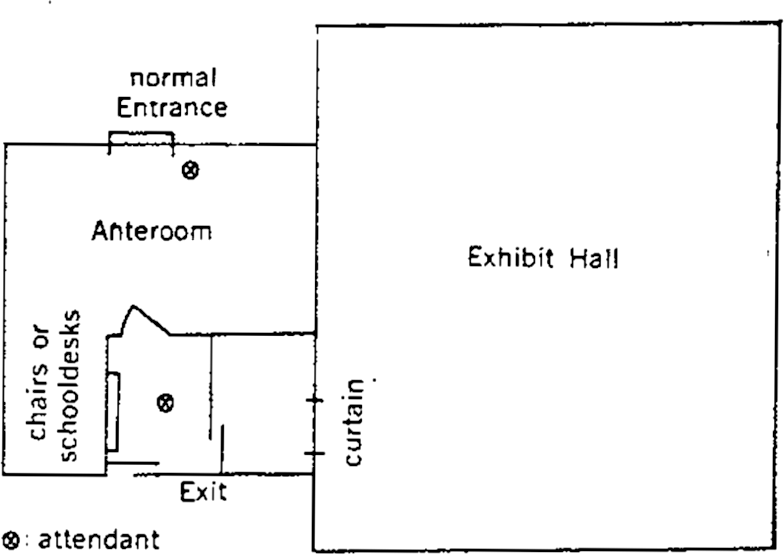
\includegraphics[scale=1]{img/dissociatordiag}\par
}

\clearpage
\newcommand\intab[1]{
\framebox[1.1\width]{\parbox[c][2.5em]{4em}{
	\centering\Huge #1}}}

\newcommand\righttab[1]{{\raggedleft\intab{#1}\par}}

\newcommand\lefttab[1]{{\raggedright\intab{#1}\par}}

{\righttab{1}

\centering

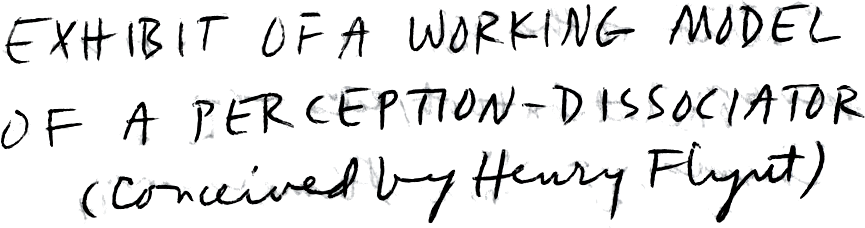
\includegraphics[width=4in]{img/guidebook_01}

\vfill


\includegraphics[width=3.5in]{img/guidebook}

\vfill

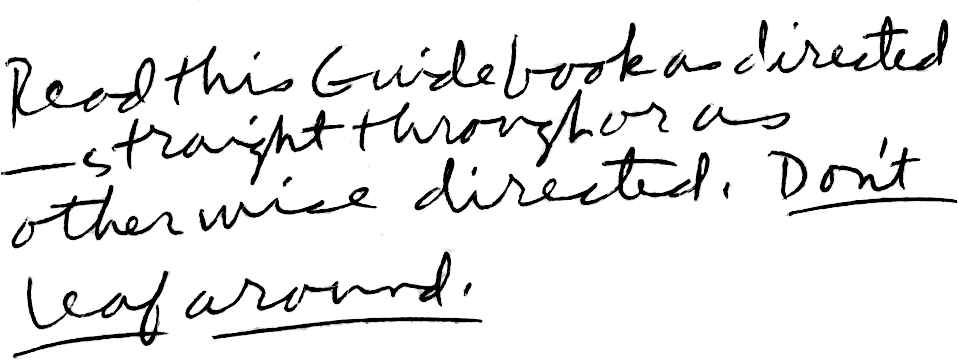
\includegraphics[width=4in]{img/guidebook_02}

\vfill

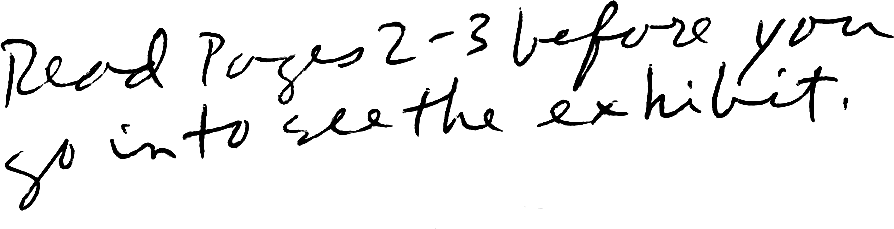
\includegraphics[width=4in]{img/guidebook_03}

\vfill\clearpage}

\lefttab{2}

\uline{Introduction.} The perception-dissociator is a machine which is the 
product of a technology far superior to that of humans. With it, a conscious 
organism can drastically transform its psychophysical relation to objects and 
to other conscious organisms. When the organism has transformed itself, 
sound disappears, time is immeasurable; and the relation between seeing and 
touching becomes a random one. That is, the organism never knows whether 
it will be able to touch or feel what it sees, and never knows whether it will 
be able to see what it touches or what touches it. The world ceases to be a 
collection of objects (relative to the physically altered organism). Further, 
the machine induces a pattern of communication in the organism's nervous 
system, an \uline{involuntary} pattern of responses to certain events, to help the 
organism cope with the invisible tactile phenomena. A dimension is added of 
involuntarily relating to other organisms as unconscious signalling devices. 
The transformation induced by the machine is permanent unless the 
organism subsequently uses the machine to undo it. 


The perception-dissociator is not conscious or alive in any human sense. 
The components of the machine that the user is aware of are: 
\begin{enumerate}
	\item Optical phenomena that are seen---\enquote{sights.} 
	\item Solid or \uline{massive} phenomena that are felt cutaneously---\enquote{touches.} 
\end{enumerate}
If the user tries to touch a sight, he may not be 
able to feel anything there. If he looks for a component that touches him, he 
may not be able to see it. 

\vfill

(Keep reading) 

\vfill

\clearpage

\righttab{3}

In other words, from the beginning the machine has properties that the 
entire world comes to have to the transformed organism. 

The exhibit spotlights the technical interest of the 
perception-dissociator, giving the visitor a working model of the machine 
which he can use to \enquote{transform} himself. Nothing is said about the purpose 
of the perception-dissociator in the society that can make one. The model is 
sophisticated enough that it can run independently of the visitor's will, and 
can affect him. In fact, the visitor may be hurt if he doesn't follow the 
instructions for using the machine. 


When you have absorbed the above, go to the entrance and be admitted 
to the exhibit. You must check your shoes, and your watch (if you have 
one), with the attendant. As you enter, turn this page and begin reading Page 
4. 

\clearpage

\lefttab{4}
\vfill 
\textsc{Do not talk or make any other uncalled-for noise.}

\vfill 

Be prepared for the touch of pulling your feet out from under you 
from behind. Don't resist; just fall forward, break your fali with your arms 
(and retrieve this Guidebook). The floor is not hard and the gravity is weak, 
so the fall should leave you absolutely unhurt. 

\plainbreak{2}

\textsc{Avoid all touches (except floor and yourself) unless directed otherwise.}


\plainbreak{2}

(You have been directed not to resist having your 
feet pulled out from under you.) 
\plainbreak{2}

\textsc{In effect, if you bump into a solid object or step on one, draw back. Remember
that you avoid touches by your tactile senses alone.}
Whether your eyes are open or closed makes no difference. It is not necessary to avoid 
sights unless you touch something. 

\plainbreak{2}

There may be the touch of being pushed forward at your shoulder 
blades. Don't resist; just move forward. 

\plainbreak{2}

As for the sights in this model, it happens that they will be humanoid. 
All the human appearances other than you in the exhibit hall are sights from 
the machine. This is just the way the model is; don't give it a thought. Sights 
may appear or disappear (for example, at the curtain) while you are looking. 

\plainbreak{2}

I am referring to the components of the model with the names of the 
components of the perception-dissociator. 

\plainbreak{2}

As soon as you understand the above and are prepared to remember 
and follow the instructions, go immediately to Page 6. 

\vfill 

\clearpage

\righttab{5}

  \vfill
\gentrisplitmath{
  \bigprobly{\jumpsover{
      \scoot{s_1}}{
      \probly{\shadows{s_2}{\eyeO{u}}}}}}{
  \jumpsover{s}{
    \jumpsover{t}{
      u}}}{
  \tackles{
    \crawl{\eyeC{u}}}{t}}
	
  \vfill
\gentrisplitmath{
  \begin{gathered}
    \shadows{s}{}\\
    \blows{t}{}
  \end{gathered}
  \:\:\:\eyeC{u}}
  {\shadows{\crouch{u}}{s_2}}
  {\jumpsover{\scoot{u}}{
    \pushes{
      \belowU{\eyeC{s_1}}}{
      \belowU{\eyeO{s_2}}}}}

  \vfill
\gentrisplitmath{
  \tackles{
    \eyeC{\crawl{u}}}{
    \eyeC{\aboveU{t}}}}
  {\probly{
    \stepson{s_1}
            {\eyeC{\crawl{s_2}}}}}
  {\crawl{t}
  \:\dfrac{\pushes{\vee}{}}{\blows{\wedge}{}}\:u}

  \vfill

\gensplitmath{\flee{\scoot{\eyeC{u}}}}
{\begin{array}{c}\begin{array}{c c}
    \pushes{s_1}{s_2}&\pushes{s_3}{s_1}\\\hline
    &\pushes{s_1}{s_2}\end{array}
  \left(\begin{array}{c}\tackles{s_1}{s_3}\\
    \jumpsover{s_2}{u}\end{array}\right)\\\:\:
  {\renewcommand{\arraystretch}{0.5}
    \begin{array}{l@{}p{8em}}
      \pushes{s_2}{s_3}\,&\hrulefill\\
      \hrulefill&\,\pushes{s_2}{s_3}\\
      \pushes{s_3}{s_1}\,&\\\end{array}}\end{array}}

\vfill

\gentrisplitmath{
	\left(
	  \begin{gathered}
            \dfrac{\tackles{\eyeC{s_1}}{s_2}}
		  {\tackles{\eyeC{s_1}}{s_2}}\\
	    \dfrac{\pushes{s_2}{s_3}}
		  {\pushes{s_2}{s_3}}
	  \end{gathered}
	\right)}
{\jumpsover{\left.\begin{gathered}
	s\\
	t
\end{gathered}\right.}{u}}{
\dfrac{\dfrac{\dfrac{\eyeC{\crawl{s_1}}}
                    {\aboveU{\eyeO{s_1}}} \: \shadows{u}{s_1}}
	     {\eyeO{\scoot{s_1}}} \: \probly{\pushes{s_1}{s_2}}}
      {\eyeO{\belowU{s}}} \: \eyeC{u}}

\vfill

\gentrisplitmath{\jumpsover{u}{\belowU{s_3}}}
  {\left(\;\begin{array}{c}
	  \jumpsover{\scoot{s_1}}{\eyeO{u} }\\
  \shadows{s_2}{u}
  \end{array}\;\right)}
  {\eyeO{s_3}}

\vfill
\gensplitmath{\jumpsover{u}{\begin{array}{c}
	\pushes{\eyeC{\belowU{s_1}}}{\eyeC{\belowU{a_1}}}\\
	\pushes{\eyeC{\belowU{s_2}}}{\eyeC{\belowU{s_1}}}
\end{array}}}{\jumpsover{\crouch{u}}{\probly{\shadows{s_1}{\eyeO{s_2}}}}}

\vfill
\gentrisplitmath{\jumpsover{t_1}{\pushes{t_2}{\scoot{u}}}}
{\shadows{s}{\shadows{u}{s}}}
{\left(\begin{array}{c}
	\jumpsover{s_2}{u} \\ \hline
	\tackles{s_1}{s_3} \\
\jumpsover{s_2}{u}\end{array}\right)
\begin{array}{c}
	\jumpsover{u}{s_1} \\ \hline
	\jumpsover{u}{s_3} \\
	\\
	\\
\end{array}}
\clearpage

% \img{dissoceqns}

\clearpage
\lefttab{6}
\section{First Phase}
You will now begin the first phase of perception-dissociation by the 
machine. Throughout this phase, you walk erect. 

Instructions for operating the machine and for protecting yourself from 
it will be given both in English and in an abbreviated symbolism. It is 
important to master the symbolism, because later instructions can't be 
expressed without it. 

\begin{itemize}
\item u means you 

\item $s$, $s_1$, $s_2$, $s_3$ mean different sights from the machine 

\item $t$, $t_1$, $t_2$, $t_3$ mean different touches from the machine 

\item $\eyeO{a}$ means $a$'s eyes are open or $a$ opens its eyes 

\item $\eyeC{a}$ means $a$'s eyes are shut or $a$ shuts its eyes 

\item $\blows{a}{b}$ means $a$ blows on $b$'s hand 

\item $\pushes{a}{b}$ means $a$ pushes $b$, typically from behind 
($a$ holds Guidebook under arm or elsewhere) 

\item $\jumpsover{a}{b}$ means $a$ jumps over $b$, crossing completely above $b$ (weak gravity should make this easy) 

\item $\shadows{a}{b}$ means $a$ rapidly waves both hands in front of and near $b$'s eyes so that 
	moving shadows are cast on $b$'s eyes ($a$ \enquote{\term{shadows}} $b$) 

\item $\tackles{a}{b}$ means $a$ pulls $b$'s ankles back and up and immediately lets them go, so 
	that $b$ falls forward ($a$ \enquote{\term{tackles}} $b$) 

\item $\stepson{a}{b}$ means $a$ jumps and falls on $b$, or $a$ steps on $b$ 

\item $\flee{a}$ means $a$ rapidly moves aside 

\item $\probly{}$ parentheses around the symbol for an action mean the action will 
probably happen 

\item A line of action symbols constitutes an instruction. The order of symbols 
indicates the order of events. If one symbol is right above another, the 
actions are simultaneous. 
\end{itemize}

\vfill
\textsc{You may always turn back to these explanations if you forget them.}

\vfill
(Keep reading) 

\vfill
\clearpage
\righttab{7}

Instructions 1--3 apply \textsc{when your eyes are open.}

\vskip 0.75em

\newcommand{\eqnAB}{
	\begin{equation*}
	\left.\begin{gathered}
		\eyeO{s_1}\\
		\eyeO{u}
	\end{gathered}\right.\:\left.
		\begin{gathered}
			\eyeC{s_1}\\
			\probly{\stepson{t}{u}}
		\end{gathered}\right.\:
	\flee{u}
	\end{equation*}}

\begin{enumerate}[label=\arabic*.,nosep, wide]
	\item \splitrule{If you see a sight close its eyes, a heavy touch from the machine may be falling toward you.
		You must instantly jump aside.}{\eqnAB}

		\vskip 0.5em

\textsc{You must follow this and succeeding instructions as long as you stay in the exhibit. Stay with each instruction until you have it thoroughly in memory; and check out the symbolic version so you learn to read the symbols.}
		\vskip 0.75em

\item \splitrule{If a sight in front of you jumps over you, a touch may be about to tackle you. You must instantly jump to one side. }{
\begin{equation*}
	\eyeO{u}\:\left.\begin{gathered}
		\jumpsover{s}{u} \\
		\probly{\tackles{t}{u}}
	\end{gathered}\:\right.\flee{u}
\end{equation*}
	}

\vskip 0.75em

\item \splitrule{If a sight waves its hands in front of your open eyes, a touch may be about to shove from behind.
	Jump to one side. }{\begin{equation*}
  \eyeO{u}\:\left.\begin{gathered}
    \shadows{s}{u}\\
    \probly{\pushes{t}{u}}
  \end{gathered}\:%
  \right.\flee{u}
\end{equation*}}


\vskip 0.75em

\textsc{If there are any sights, try standing around and following these instructions for a short while.}

\vskip 0.75em

\item \splitrule{If you close your eyes, you must keep them closed until a touch tackles you, a touch shoves you, or you can't keep your mind on the exhibit (which you should also consider to be an effect of the machine). Then you immediately open your eyes.}{\begin{equation*}
    \quad\eyeC{u}\:%
      \dfrac{\tackles{t}{u}}{
        \dfrac{\pushes{t}{u}}{
          u\:\text{inattentive}}}%
  \:\eyeO{u}
\end{equation*}}

\vskip 0.75em

\emph{(A horizontal line between action symbols means \emph{or.} With it, instructions can be combined)}

\vskip 0.75em

\textsc{The next three instructions tell you what to do when your eyes are closed. Learn them well.}

\vskip 0.75em

\item \splitrule{If you feel a breath blowing on one of your hands, a touch may be falling on you. You must instantly jump to the side away from the breath.}{\begin{equation*}
  \eyeC{u}\:\begin{gathered}
    \blows{t_1}{u}\\
    \probly{\stepson{t_2}{u}}
  \end{gathered}
  \flee{u}
\end{equation*}}

\vfill

\textit{(Turn page and continue) }

\vfill

\clearpage

\lefttab{8}

\vfill
\item If your closed eyes are shadowed, a touch may be about to tackle 
you. You must instantly jump aside. 
\begin{equation*}
  \eyeC{u}\begin{gathered}
    \shadows{s}{u}\\
    \probly{\tackles{t}{u}}
  \end{gathered}
  \:\:\flee{u}
\end{equation*}

\vfill
\item If you sense a massive touch going above your head, another touch 
may be about to shove you from behind. Jump aside. 

  \[\eyeC{u}\:\begin{gathered}
    \jumpsover{t_1}{u}\\
    \probly{\pushes{t_2}{u}}
  \end{gathered}
  \:\:\flee{u}\]

\vfill
\item If you have any time left over from following other instructions, 
close your eyes and go around with your hands in front of you, shoving 
touches whenever you feel them. 

\[\eyeC{u} \:\:\: \pushes{u}{t}\]

\vfill

\textsc{Now try instr. 8, remembering and following the other instructions about closed eyes (instr. 4--7).
When you have to open your eyes again, as per instr. 4, check anything you forgot: and then go to the
succeeding instructions. Now---close your eyes.}

\vfill

\textsc{The next three instructions apply when your eyes are open.}

\vfill
\item If you see a sight falling toward or about to step on another sight 
whose eyes are open, run until you face the sight on the ground and close 
your eyes. 

\textsc{Before you follow this instruction you must have mastered the preceeding instructions about closed eyes.}

\[\eyeO{u}\:\eyeO{s_2}\:\probly{\stepson{s_1}{s_2}}\:\eyeC{u}\]

\vfill
\textit{(Keep going) }

\clearpage

\righttab{9}

\vfill
\item If you see a sight about to tackle another whose eyes are \uline{open}, run 
until you face the sight about to be tackled and jump over both sights. If the 
sight about to be tackled has \uline{closed eyes}, you must immediately shadow 
them. 

\vfill
  \[\eyeO{u}\dfrac{%
      \eyeO{s_2}\quad\probly{\tackles{s_1}{s_2}}\quad\jumpsover{u}{s_1 s_2}%
    }{%
      \eyeC{s_2}\quad\probly{\tackles{s_1}{s_2}}\quad\shadows{u}{s_2}%
    }\]

\vfill
\item If you see a sight about to push another with open eyes from 
behind, you must shadow the sight about to be pushed. But if the sight 
about to be pushed has closed eyes, you must immediately jump over both 
sights. 


\vfill

  \[\eyeO{u}\dfrac{%
    \eyeO{s_2}\quad\probly{\pushes{s_1}{s_2}}\quad\shadows{u}{s_2}
    }{%
      \eyeC{s_2}\quad\probly{\pushes{s_1}{s_2}}\quad\jumpsover{u}{s_1 s_2}
    }\]

\end{enumerate}

\vfill
You must now put all the instructions into practice until you have 
learned them thoroughly by doing as they say. In other words, carry out 
Instr. 8, and the other instructions as they apply. 

\vfill
If you can't practice the instructions because you still have not seen a 
sight or felt a touch, skip directly to Page 18. 

\vfill

Learning the instructions in practice should take a good while. When 
you have mastered them, the first phase is over. Turn to Page 10 and \textit{begin the second phase}.

\vfill

\clearpage

\lefttab{10}

\section{Second Phase}

\vfill
You are now in the second phase of transforming yourself with the 
perception-dissociator. Throughout this phase, you must stoop or crouch 
somewhat. That is, you must keep yourself below the height of your neck 
when you stand straight---except when you jump over a sight. The symbol is 
$\crouch{u}$. $\eyeC{\crouch{u}}$ means that you crouch and close your eyes. \emph{Now crouch.}

The numbered instructions for this phase are so similar to those in the 
preceeding phase that they will be given in symbols only. Changes are noted 
parenthetically. You may turn back if you forget symbols. 

\vfill
\begin{enumerate}
	\gensplit{\item\BEQ{
	\left.\begin{gathered}
	\eyeO{s_1}\\
	\eyeO{\crouch{u}}
	\end{gathered}\right.
	\:\:
		\left.\BG{
		\eyeC{s_1}\\
		\probly{\stepson{t}{u}}
	}\right.
	\:\:
		\flee{u}}}
{\item\BEQ{
	\eyeC{\crouch{u}}\:
		\BG{\jumpsover{s}{u}\\
		\probly{\tackles{t}{u}}}\:
		\flee{u}}}

\vfill
\gensplit
  {\item\BEQ{\eyeC{\crouch{u}}\:
	     \BG{\blows{t}{u}\\
		 \pushes{t_2}{u}}\:
             \flee{u}}}
 {\emph{(change: component blows on you instead of shadowing you)}}

\vfill
\gensplit{\item\BEQ{
  \eyeC{\crouch{u}}\:\:
  \dfrac{\tackles{t}{u}}
	{\dfrac{\pushes{t}{u}}
	       {u\:\text{inattentive}}}\:\:
  \flee{u}}}
  {\item\BEQ{
  \eyeC{\crouch{u}}\:\:
  \BG{\blows{t_1}{u}\\
      \probly{\tackles{t_2}{u}}}\:\:
  \flee{u}}}


\vfill
\gensplit{\item\BEQ{
  \eyeC{\crouch{u}}\:\:
  \BG{\shadows{s}{u}\\
      \probly{\tackles{t}{u}}}\:\:
  \flee{u}}}
  {\item\BEQ{
  \eyeC{\crouch{u}}\:\:
  \BG{\jumpsover{t_1}{u}\\
      \probly{\pushes{t_2}{u}}}\:\:
  \flee{u}}}

\vfill
\gensplit{\item\BEQ{
  \eyeC{\crouch{u}}\qquad\pushes{u}{t}}}
{The big change comes next. 
\plainbreak{2}
\emph{(Keep going)}}

\vfill

\clearpage
\righttab{11}

\vfill
\item \BEQ{\begin{array}{c c c c r}
		\eyeO{\crouch{u}} &
		  \eyeO{s_2} &
		  \probly{\stepson{s_1}{s_2}}& 
		  \eyeC{u} & \text{\uline{and also}} \\
		\eyeO{\crouch{u}} &
		  \eyeC{s_2} &
		  \probly{\stepson{s_1}{s_2}} & 
		  \blows{u}{s_2} & \end{array}}

\vfill
That is, if you see a sight falling or stepping on another sight with \uline{closed eyes}, you must immediately blow on the sight on the ground. This is an addition.
\vfill
\item \[
  \eyeO{\crouch{u}}\:\:
  \begin{array}{c c c}
    \eyeO{s_1} & \probly{\tackles{s_1}{s_2}} &
      \jumpsover{u}{s_1 s_2} \\
    \hline
    \eyeC{s_1} & \probly{\tackles{s_1}{s_2}} &
      \shadows{u}{s_2} \\
  \end{array}
\]

\vfill
\splitshort{\item \[
  \eyeO{\crouch{u}}\:\:
  \begin{array}{c c c}
	  \eyeO{s_2} & \probly{\pushes{s_1}{s_2}} & \blows{u}{s_2} \\
	  \hline
	  \eyeC{s_2} & \probly{\pushes{s_1}{s_2}} & \jumpsover{u}{s_1 s_2} \\
  \end{array}\]}
  {\emph{(change: you blow on $s_2$)}}

\vfill
So far there have been only three changes in the instructions. Memorize 
them. Then go on to Instr. 12, which is new, and carry it out along with the 
other eleven instructions. 

\vfill
\textsc{As soon as you have put any changed instruction (3, 9, or 11) into practice,
the second phase is over. Turn to page 12 and the third phase.}

\vfill
If you can't practice the instructions because all the components have 
vanished, skip to Page 18. 

\vfill

\splitrule{\item Adding to Instruction 8, if you have time left over from following other instructions, you may also keep your eyes open and jump over, blow on, or shadow sights.}{\[
	\eyeO{\crouch{u}}\:\:
	\begin{array}{c}
		\jumpsover{u}{s} \\ \hline
		\shadows{u}{s} \\ \hline
		\blows{u}{s} \\
	\end{array}
\]}
\end{enumerate}

\clearpage 

\lefttab{12}

\section{Third Phase}

Throughout the third phase, you must squat or move on your hands 
and knees. That is, you must always keep yourself below the height of your 
waist when you stand straight---unless you are able to jump over a sight from 
your low position. The symbol is $\crouch{u}$. Now get down. 

Instr. 1--7 from the last phase apply here without change. They are thus 
stated in the most abbreviated form. 

\vfill

{1--3. \parbox[t]{1.75in}{\[
	\eyeO{\crouch{u}} \:\: 
	\begin{array}{c}
		\eyeC{s} \\
		\probly{\stepson{t}{u}} \\ \hline
		\jumpsover{s}{u} \\
		\probly{\tackles{t}{u}} \\ \hline
		\blows{t_1}{u} \\
		\probly{\pushes{t_2}{u}}
	\end{array}\:\:
	\flee{u}
\]\vskip 3.5em} 4--7. \parbox[t]{2.4in}{\[
	\eyeC{\crouch{u}}\:\:
	\dfrac{
		\:\:
	  \begin{array}{c}
	    \tackles{t}{u} \\ \hline
	    \pushes{t}{u} \\ \hline
	    u \:\:\text{inattentive} \\
	  \end{array}\qquad
	\eyeO{u}\:\:}
{\begin{array}{c}
	    \blows{t_1}{u} \\
	    \probly{\stepson{t_2}{u}} \\ \hline
	    \shadows{s}{u} \\
	    \probly{\tackles{t}{u}} \\ \hline
	    \jumpsover{t_1}{u} \\
	    \probly{\pushes{t_2}{u}} \\
	 \end{array}\qquad
	 \flee{u}}
 \]}

\vfill
The biggest change comes next. 

\vfill
8. If you have any time left over, close your eyes and go around with 
your hands in front of you. If you encounter touches standing higher than 
you, tackle them. If you encounter touches as near the ground as you, shove 
them. You must be sensitive and judge heights with eyes closed. 

\vfill

\[
	\eyeO{\scoot{u}}\:\:\begin{array}{c c}
		\aboveU{t} \tackles{u}{t} \\ \hline
		\belowU{t} \pushes{u}{t} \\
	\end{array} \:\:
	\left( \begin{gathered}
		\aboveU{t} \: \text{\textsc{means "if $t$ stands high relative to you"}} \\
		\belowU{t} \: \text{\textsc{means "if $t$ is near ground relative to you"}}
	\end{gathered} \right)
	\]

	\vfill

9. \parbox{1.5in}{No change.}\parbox{2in}{\[
	\eyeC{\scoot{u}} \:\: \begin{array}{c c c}
		\eyeC{s_2} & \probly{\stepson{s_1}{s_2}} & \eyeO{u} \\ \hline
		\eyeO{s_2} & \probly{\stepson{s_1}{s_2}} & \blows{u}{s_2}
	\end{array}
\]}
\vfill

\vfill
(Keep going) 

\clearpage
\righttab{13}

\vfill 

10. \gensplit{The previous Instr. 10 applies if $s_2$ is near the ground, that is, it applies unless $s_2$ is too high for you to jump or shadow it.}{\[
	\eyeC{\scoot{u}} \: \begin{array}{c c c}
		\belowU{\eyeC{s_2}} & \probly{\tackles{s_1}{s_2}} & \jumpsover{u}{s_1 s_2} \\ \hline
		\belowU{\eyeO{s_2}} & \probly{\tackles{s_1}{s_2}} & \shadows{u}{s_2}
	\end{array}
\]}

\vfill 

11. \gensplit{\[
	\eyeC{\scoot{u}} \:\: \eyeC{s_2} \:\: \probly{\pushes{s_1}{s_2}} \:\: \blows{u}{s_2}
\]}{The second half of the previous Instr. 11 is dropped. }

\vfill 
\vskip 1.5em
Except for the instruction to tackle touches, the changes are simply 
limitations to make the instructions feasible for $u\sfrac{1}{2}$. They should be easy 
to remember. 

\vskip 1.5em

You will next go on to Instr. 12, and carry it out along with the other 
instructions. As soon as you encounter an actual situation where you cannot 
act because $u\sfrac{1}{2}$, the third phase will be over. 
\textsc{At that point you must turn to page 14 and the fourth phase.}

\vskip 1.5em
If you can't carry out the instructions because all the components have 
vanished, the third phase is over. Turn to Page 14 and the fourth phase. 

\vskip 1.5em

\vfill 

12. \gensplit{Adding to Instr. 8, if you have time left over, you may also keep 
your eyes open and blow on sights. You may also shadow or jump over 
sights unless they are too high. }{ \vfill 
\[\eyeC{\scoot{u}} \:\: \dfrac{\blows{u}{s}}{
	\belowU{s} \:\: \dfrac{\blows{u}{s}}{\jumpsover{u}{s}}}
\]}
\vfill 
\clearpage
\lefttab{14}

\section{Fourth phase}



You are in the fourth phase of perception-dissociation. Throughout this 
phase, you must crawl on your stomach (keep below knee height). The 
symbol is $u\sfrac{1}{4}$. Now get on the floor. 

You can no longer be tackled, nor can you jump. Thus, the numbered 
instructions are greatly limited, and they will be restated fully. 

\vfill

\textsc{The first two instructions apply when your eyes are open.}

\vfill

\begin{enumerate}
\gensplit{\item If you see a sight close its eyes, a touch may be falling or stepping on you, and you must immediately scramble aside.}
{\[\begin{array}{c c}
	\eyeO{s_1} & \eyeC{s_1} \\
	\eyeO{\crawl{u}} & \probly{\stepson{t}{u}}
\end{array} \:\: \flee{u}\]}

\vfill

		{\centering \parbox{2in}{
\item \[ \eyeO{\crawl{u}} \:\: \begin{array}{c}
		\blows{t_1}{u} \\
\probly{\pushes{t_2}{u}} \end{array} \:\: \flee{u} \]}\par}

\vfill

\textsc{The next three instructions tell you what to do when your eyes are closed.}

\vfill

\gensplit{\item When to reopen your eyes.}{\[
		\eyeC{\crawl{u}} \:\: \begin{array}{c}
			\pushes{t}{u} \\ \hline
			u \:\: \text{inattentive} \\
		\end{array} \:\: \eyeO{u}\]}

\vfill

\gensplit{\item If your closed eyes are \uline{shadowed}, a touch may be falling or stepping on you. Scramble aside.}
	{\[ \eyeC{\crawl{u}} \:\: \begin{array}{c}
		\blows{t_1}{u} \\
	\probly{t_2}{u} \end{array} \:\:
		\flee{u} \]}

		\vfill

\gensplit{\item \[
	\eyeC{\crawl{u}} \:\: \begin{array}{c}
		\jumpsover{t_1}{u} \\
	\probly{\pushes{t_2}{u}} \end{array} \:\:
		\flee{u} \]}{
\item \[ \eyeC{\crawl{u}} \:\:
		\begin{array}{c c}
			\aboveU{t} & \tackles{u}{t} \\ \hline
		\crawl{t} & \pushes{u}{t} \end{array} \]}

		\vfill
\textsc{Try instr. 6, remembering and following instr. 3--5.} \\
\textsc{When you have to reopen your eyes as per instr. 3, check on anything you forgot.
	Then go to page 15. Now---close your eyes.}

\vfill

\clearpage
\righttab{15}

The rest of the instructions apply when your eyes are open. 


\vfill

\item \gensplit{\[
		\eyeO{\crawl{u}} \:\: \begin{array}{c c c}
			\eyeO{s_2} & \probly{\stepson{s_1}{s_2}}
			& \eyeC{u} \\ \hline
		\belowU{\eyeC{s_2}} & \probly{\stepson{s_1}{s_2}} & 
			\shadows{u}{s_2}
		\end{array} \]}{If $s_2$'s eyes are closed, you must shadow them unless they are too high. }

\vfill
\item \gensplit{\[
\eyeO{\crawl{u}} \:\: \belowU{\eyeO{s}} \:\:
\probly{\pushes{s_1}{s_2}} \:\: \blows{u}{s_2}\]}{You blow on $s_2$'s hand unless it is too high.}

\vfill
\gensplit{\item Adding to Instr. 6, if you have time left over from following instructions, you may also shadow or blow on sights if they aren't too high.}{\[
\eyeC{\crawl{u}} \: \belowU{s} \: \dfrac{\shadows{u}{s}}{\blows{u}{s}}\]}

\vfill

You must now put these nine instructions into practice until you have 
learned them thoroughly in practice; and even continue after that until you 
have difficulty keeping your mind on the exhibit. 

\vfill

\textsc{If you can't practice the instructions because all the components have vanished, skip to page 18.}

\vfill

Otherwise, stay with this phase until you have difficulty keeping your 
mind on it. Then turn to Page 16 and the final phase of 
perception-dissociation. 

\vfill
\end{enumerate}

\clearpage
\lefttab{16}

\vfill
\section{Final Phase}

\vfill
You are now in the final phase of transforming yourself with the 
perception-dissociator. When you finish transforming yourself, you will have 
lost track of time, and will have ceased to notice sound. You will be dealing 
with sights and touches as unrelated phenomena; and you will be responding 
by reflex action to unconscious signals from "other people." 

For this last phase, you will turn to Page 5. You will go through the 
symbols there in any order you like as if they were one long instruction, 
carrying out that instruction. You are to "use" each symbol once. There 
have been enough precedents in the interpretation of the symbols that you 
should now be able to interpret any combination of them. Continue to 
follow the previous numbered instructions as they apply, depending on 
whether you are 1, \sfrac{3}{4}, \sfrac{1}{2}, or \sfrac{1}{4}. 
(But forget the instructions for time left 
over; you won't have any extra time.) 
\textsc{Remember the instructions about when to reopen your eyes if you close them.}

When you are through, you will be transformed. 
\textsc{Now turn to page 5 and begin.}

\vfill

\clearpage
\righttab{17}

\vfill

If you have found these words and are reading them in desperation 
because you are completely confused; or because you have lost interest in 
the exhibit; or because you have finished; then you are transformed. 


If you want to use the model to simulate the reversal of your 
transformation before you leave the exhibit, do the following. Spend 50 
seconds erect, with open eyes, walking up to sights and pushing 
them---assuming that you will find touches where you see sights. Count the 
seconds "one-thousand-and-one," "one-thousand-and-two," etc. 


Then you will close your eyes. If you are blown on or pushed before 
250 seconds have passed, you will open your eyes and--assuming that you 
will find a sight where you were touched--you will shadow it. Otherwise you 
will open your eyes when the 250 seconds have passed. Now close your eyes 
and do as instructed. 


\vfill
It is now suggested that you leave the exhibit. Go out through the 
curtain. 

\vfill
\clearpage
\lefttab{18}

\vfill
Stay in the exhibit and follow every instruction that is relevant, until
you become thirsty. 


If you begin to encounter components, return to the page you were on 
before you turned to this one. 


lf you still don't encounter components, the model must be broken. 
Leave the exhibit by the same passage through which you entered. 

\vfill 
\clearpage


\chapter{Mock Risk Games}


Suppose you stand in front of a swinging door with a nail sticking out of it 
pointing at your face; and suppose you are prepared to jump back if the 
door suddenly opens in your face. You are deliberately taking a risk on the 
assumption that you can protect yourself. Let us call such a situation a "risk 
game." Then a mock risk game is a risk game such that the misfortune which 
you risk is contrary to the course of nature, a freak misfortune; and thus 
your preparation to evade it is correspondingly superficial. 

If the direction of gravity reverses and you fall on the ceiling, that is a 
freak misfortune. If you don't want to risk this misfortune, then you will 
anchor yourself to the floor in some way. But if you stand free so that you 
can fall, and yet try to prepare so that if you do fall, you will fall in such a 
way that you won't be hurt, then that is a mock risk game. if technicians 
could actually effect or simulate gravity reversal in the room, then the risk 
game would be a real one. But I am not concerned with real risk games. I am 
interested in dealing with gravity reversal in an everyday environment, where 
everything tells you it can't possibly happen. Your 'preparation' for the fall 
is thus superficial, because you still have the involuntary conviction that it 
can't possibly happen. 

Mock risk games constitute a new area of human behavior, because they 
aren't something people have done before, you don't know what they will be 
like until you try them, and it took a very special effort to devise them. 
They have a tremendous advantage over other activities of comparable 
significance, because they can be produced in the privacy of your own room 
without special equipment. Let us explore this new psychological effect; and 
let us not ask what use it has until we are more familiar with it. 

Instructions for a variety of mock risk games follow. (I have played 
each game many times in developing it, to ensure that the experience of 
playing it will be compelling.) For each game, there is a physical action to be 
performed in a physical setting. Then there is a list of freak misfortunes 
which you risk by performing the action, and which you must be prepared 
to evade. The point is not to hallucinate the misfortunes, or even to fear 
them, but rather to be prepared to evade them. First you work with each 
misfortune separately. For example, you walk across a room, prepared to 
react self-protectingly if you are suddenly upside down, resting on the top of 
your head on the floor. In preparing for this risk, you should clear the path 
of objects that might hurt you if you fell on them; you should wear clothes 
suitable for falling; and you should try standing on your head, taking your 
hands off the floor and falling, to get a feeling for how to fail without 
getting hurt. After you have mastered the preparation for each misfortune 
separately, you perform the action prepared to evade the first misfortune 
and the second (but not both at once). You must prepare to determine 
instantly which of the two misfortunes befalls you, and to react 
appropriately. After you have mastered pairs of misfortunes, you go on to 
triples of misfortunes, and so forth. 

The principal games are for a large room with no animals or distracting 
sounds present. 

\textbf{A.}Walk across the lighted room from one corner to the diagonally 
opposite one, breathing normally, with your eyes open. 
\begin{enumerate}
\item You are suddenly upside down, resting on the top of your head on the 
floor. You must get down without breaking your neck. 

\item Although the floor looks unbroken and solid, beyond a certain point 
nothing is there. If you step onto that area, you will take a fatal fall. Thus, as 
you walk, you must not shift your weight to your forward foot until you are 
sure it will hold. Put the ball of the forward foot down before the heel. 

\item Something happens to the cohesive forces in your neck so that if your 
head tips in any direction, it will come right off your body, killing you 
immediately. Otherwise everything remains normal. Thus, as you walk, you 
must "balance" your head on your neck. When you reach the other side of 
the room, your neck will be restored to normal. (Prepare beforehand by 
walking with a book balanced on your head.) 

\item Invisible conical weights fall around you with their points down, each 
whistling as it falls. You must evade them by ear in order not to be stabbed. 
Walk softly and fast. 

\item The room is suddenly filled with water. You have to control your lungs 
and swim to the top. Wear clothes suitable for swimming. 
\end{enumerate}

\textbf{A'.} Play game A while on a long walk on an uncrowded street. The floor 
is replaced by the sidewalk. The fifth misfortune becomes for space suddenly 
to be filled with water to a height of fifteen feet above the street. 

\textbf{B.} Lie on your back on a pallet in the dimly lit room, hands at your 
sides, with a pillow on your face so that it is slightly difficult to breathe, for 
thirty seconds at a time. 
\begin{enumerate}
\item The pillow suddenly hardens and becomes hundreds of pounds heavier. It 
remains suspended on your face for a split second and then "falls," bears 
down with full weight. You must jerk your head out from under it in that 
split second. 

\item The pillow adheres to your skin with a force greater than your skin's 
cohesion, and begins to rise. You must rise with it in such a way that your 
skin is not torn. 
\end{enumerate}

\textbf{C.} Lie on your back on the pallet in the dimly lit room. 

\begin{enumerate}
\item Gravity suddenly disappears completely, so that nothing is held down by 
it; and the ceiling becomes red-hot. You must avoid drifting up against the 
ceiling. 

\item The surface you are lying on becomes a vast lighted open plane. From the 
distance, giant steel spheres come rolling in your direction. You must evade 
them. 

\item Your body is split in half just above the waist by an indefinitely long, 
rather high, foot-thick wall. Your legs and lower torso are on one side, and 
your upper torso, arms, and head are on the other side. Matter normally 
exchanged between the two halves of your body continues to be exchanged 
through the. wall by telekinesis. It is as if you are a foot longer above the 
waist. In order to reunite your body, you must first roll over and get up, 
bent way forward. There are depressions in the wall on the same side as your 
feet. You have to climb the wall, putting your feet in the depressions and 
balancing yourself. You will be reunited when you reach the top and your 
waist passes above the wall. 
\end{enumerate}

\textbf{D.} Sit in a plain, small, straight chair, on the edge of the seat, hands 
hanging at the sides of the seat, feet together in front of the chair, in the 
lighted room, for about thirty seconds at a time. 

\begin{enumerate}
\item The chair is suddenly out from under you and sitting on you with Its legs 
straddling your lap and legs. You have to get your weight over your feet so 
you won't take a hard fall. 

\item The direction of gravity reverses and the chair remains anchored to the 
floor. You have to grab the seat and hold on in order not to fall on the 
ceiling. 

\item You are suddenly in a contra-terrene universe, in which the atmosphere is 
unbreathable and prolonged contact with either the atmosphere or the 
ground will disintegrate you. The seat and back of the chair become a 
penetrable hyperspatial sheet between the alien universe and your own. As 
soon as you feel the alien atmosphere, you must jerk your feet off the 
ground and deliberately sink or plunge through the seat and back of the chair 
in the best way that you can. You will end up on the floor under the chair in 
your universe. 

\item You are suddenly in dark empty space in a three-dimensional lattice of 
gleaming wires. Segments of the lattice alternately burst into flame and cool 
off. You adhere to the chair as if it were part of you. With your hands 
holding onto the seat, you can move yourself and the chair forward by 
pushing the seat forward with your hands; you can move backward by
pulling backward; you can move up by pulling up on the seat; and so on.
The lattice is formed in such a way that in order to move from one cell to
the next, you always haave to turn to some extent. Flames immediately
spring up next to you, and you have to maneuver yourself through the 
lattice to escape them.
\end{enumerate}

\textbf{D`.} Play Game D in situations where you have to sit and wait.

Note: The original version of \essaytitle{Mock Risk Games} was entitled 
\essaytitle{Exercise Awareness-States}. It was written during April--July, 1961; and
read at the AG Gallery in New York on July 15, 1961. I subsequently turned
against amusemental compositions, and around June 25, 1962 I sent the
only copy of \essaytitle{Exercise Awareness-States} to the young musician Tom
Constanten, at 1650 Michael Way in Las Vegas. I later wrote Constanten 
asking him to return the MS, but I never heard from him. The present revival
analyses the activity better than the original version did. I am unable,
though, to remember some of the most elegant misfortunes for the original
games (A, B, C); and it seems that they are permanently lost.

In developing the original games---and the present games---I had two
objectives in mind. First, the experience of playing the games (as opposed to
reading or analyzing them) must involve or compel you, must be vivid and
immediate. Secondly, the misfortunes must be elegant, undreamed-of
"explosions" of the natural order. These objectives, though, do not
constitute a use for the games. The games can have many uses, beginning
with amusement; and it remains to be seen what the most significant use will
be.

\section*{Intrusions}

A noise in an adjacent room may intrude on a person playing a mock
risk game, and affect his experience or state of being in a variety of ways.
Let us consider the effects of such \enquote{intrusions} on the player's state. There
are several kinds of intructions. \enquote{Distractions} are perceived by the player to
be unrelated to the game, and tend simply to take his mind off it. \enquote{Bogies}
are surprises which so fit in with the game that the player momentarily
thinks a freak misfortune has really begun; they tend to frighten the player 
and halt the game. \enquote{Modulations} are changes in the player's state or mood
which may enhance the game; they are typically induced with drugs.

The player himself can turn the radio on, bring in a cat, or otherwise
create distractions for himself. Here the object of study is how compelling
the game is. Through how much distraction can the game hold the player's 
attention? Turning to modulations, the player can also produce them for
himself.

More elaborate investigations require an experimenter outside a room
where the subject is playing mock risk games. The experimenter needs a
one-way window and an intercom to observe and talk with the subject. Here
the effects of bogies can be studied. (The experimenter has a problem 
though, in that after he frightens the subject, the subject will forget about
the game and just watch out for the bogies.) Here are some sample bogies,
for game A:
\begin{enumerate}
	\item Trip the subject with an invisible thread.
	\item Cause the floor to shift.
	\item Throw a pingpong ball at the subject from the side.
	\item Squirt water on him from behind.
\end{enumerate}
The mechanics of the experiments can readily be 
worked out by anyone interested in them. After an intrusion, the 
experimenter should question the subject about his reaction if it is
appropriate.

\section*{Mock Risk Games for Couples (Duo Games)}

In order for these games to 
be successful,  each of you has to have confidence that the other is actually
playing. If you lack this confidence, you forget the game and just watch out
for intrusions created by the other.

\textbf{AA.} Face each other at a distance and walk toward each other.
\begin{enumerate}
	\item The other's head flies off and hurtles at you like a cannonball. It can
		swerve up or down, so that you will be hit unless you jump aside. The time
		you have to jump is about the same no matter what your distance from the
		other is, because the head accelerates rapidly.
	\item Just as the other is putting his foot down to make a step, he suddenly
		becomes so large that his foot is descending right over your head. At the 
		same time, the mental commands of each of you to your muscles begin to be
		transmitted to the other's muscles rather than your own, and to be executed
		by his muscles rather than by yours. Thus, you must jerk "your" / "his" foot
		back, rather than complete the step, in order not to "step on your own
		head." The two of you should walk in step, right foot with right and left 
		with left. Watch the other's feet and also watch above yourself---using your
		vertical peripheral vision to do so. In short, if you suddenly see a giant foot
		coming down on you, jerk "your" forward foot back.
	\item (This misfortune is exceptionally complex, but there are good reasons for
		the complexity, and it will repay study.) The consciousness of each of you
		suddenly becomes located in the other's body and becomes hooked into the 
		other's receptors and muscles. At the same time, your body, which is now
		"outside you" and which is under the other's control, becomes surrounded
		by slowly moving beams of tissue-destroying radiation coming from the sides
		of the room. The radiation is invisible, but the eyes you are seeing through
		become sensitive to it. At the same time, the other mind loses its knowledge
		of language. In order to save your body, under the other's blind control,
		from blundering into a radiation beam, you have to communicate 
		pre-verbally to the other mind by every means from vocal cries to 
		pantomine, and get your-body/his-mind out of range of the radiation. When 
		the body is out, you will both be restored to normal. (The first thing to 
		anticipate is the basic shift in viewpoint by which you will be looking at 
		your own body from the other's position. There is no point in tensing your 
		muscles in preparatiton for the misfortune, because if it occurs, you will be 
		working with a strange set of muscles anyway. The next thing to prepare to 
		do is to spot the radiation beams; and then to yell, gesture, or 
		whatever--anything to get the "other" to avoid the radiation. Note finally 
		that neither player prepares for the possibility that he will be surrounded by 
		radiation. Each player prepares for the same role in an asymmetrical pas de 
		deux.) 
\end{enumerate}

\emph{Asymmetry:} The two of you play a given duo game, but each prepares 
to evade a different misfortune. 

\textbf{AB.} Stay awake with eyes closed for an agreed upon time between one 
and fifteen minutes. Use a timer with an alarm. 

\begin{enumerate}
\item Each suddenly has the other's entire present consciousness in addition to 
his own, from perceptions to memories, ideologies, ambitions, and 
everything else---threatening both with psychological shock. 

The couple must take up positions such that their sensory perceptions 
are as nearly identical as possible. Beforehand, each must discuss with the 
other the aspects of the other's attitude to the world which each must fears 
having impused on his consciousness. During the game, each must think 
about these aspects and try to prepare for them. 

\item Each suddenly relives the other's most intense past feelings of depression 
and suicidal impulses. In other words, if five years ago the other attempted 
suicide because he failed out of college, you suddenly have the consciousness 
that "you" have just failed out of college, are totally worthless, and should 
destroy yourself. Presumably the other has since learned to live with his past 
disasters, but you do not have the defenses he has built up. You are 
overwhelmed with a despair which the other felt in the past, and which is 
incongruous with the rest of your consciousness. In summary, both of you 
risk shock and suicidal impulses. Beforehand, of course, each must tell the 
other of his worst past suicidal or depressed episode; and discuss anything 
else that may minimize the risk of shock. 
\end{enumerate}

\section*{Intrusions in Duo Games}

As before, distractions and modulations can be openly studied by 
consent of the players. As for bogies, it is possible in duo games for one 
player to create a bogy without warning, in effect acting as a saboteur. As 
soon as a game is sabotaged, though, confidence is lost, and each player just 
watches out for the other's bogies. Here are some sample intrusions. 

\begin{tabular}{ r c c p{2in} }
	\textsc{Game} & \textsc{Distraction} & \textsc{Bogy} & \textsc{Modulation} \\
	AA 1. & cough & shout in other's face & each take a different drug \\
	2. & talk and laugh \linebreak get out of step & $\rightarrow$ \linebreak (stomp hard) & \\
	3. & spin around & $\rightarrow$ & \\
	AB 1. & cough \linebreak talk and laugh & gasp \linebreak silently pass palm back \& forth in front of other's face & \\
	2. & & & \\
\end{tabular}



\chapter{The Dream Reality}

\section{Memo on the Dream Project}

Original aim: To recreate the effect of e.g. Pran Nath's singing---transcendent 
inner escape---in direct life rather than art. I needed material which could 
function as an alien civilization (since the source of Pran Nath's expression is 
an alien civilization relative to me); yet which was encultured in me and not 
an affectation or pretense. I decided to use dreams as the material, assuming 
that my dreams would take me to alien worlds. But mostly they did not. 
Mostly my dreams consist of long periods of tawdry, familiar life interrupted 
occasionally by senseless, unmotivated anomalies. In contrast, my original 
aim required alluring, psychically gratifying material. 

The emphasis shifted to redefining reality so that dreams were on the same 
level as waking life; so that they were apprehended as what they seem to be: 
literal reality (and not memory, precognition, or symbolism). The project 
was still arcane, but in a drastically different way. I was getting into an 
alternate reality which was extremely bizarre but not psychically gratifying. 
It was boringly frightful and sometimes obscene. I became concerned with 
analytical study of the natural order of the dream world, a para-scientific 
investigation. As I grappled with the rational arguments against treating 
dreams as literal reality, the project became a difficult analytical exercise in 
the philosophy of science. The original sensuous-esthetic purpose was lost. 

Now I would like to return to the original aim, but how to do it? Obtain 
other people's dreams---see if they are more suitable? Work only with my 
very rare dreams which do take me to alien worlds? Try to alter the content 
of my raw dreams? Attempt to affect content of dreams by experiment in 
which many people sleep in same room and try to communicate in their 
sleep? The most uncertain approach to a solution: set up a transformation 
on my banal dreams, so that to the first-order activity of raw dreaming is 
added a second-order activity. The transformation procedure to somehow 
combine conscious ideational direction---coding of the banal dreams---with 
alteration of my experience, my esthesia, my lived experience. 

\section{Dreams and Reality---An Experimental Essay}

Excerpts from my dream diary which are referred-to in the essay that 
follows. 

\dreamdate{12/11/1973}

I notice a state between waking and dreaming: a waking dream. I have 
been asleep; I wake up; I close my eyes to sleep again. While not yet asleep, I 
experience isolated objects before me as in a dream, but with no 
background, only a dark void. In this case, there are two pocket combs, both 
with teeth broken. In the waking world, I threw away one of my two pocket 
combs because I broke it; the other comb is still in good condition. 

\dreamdate{12/30/1973}

I am chased by the police for one block west on West Market Street in 
Greensboro. I reach the intersection with Eugene Street, and in the north 
direction there is a steep hill rather than the street. The surface of the hill is 
bare ground and grass. I run up the hill, sensing that if I can get over the hill 
I will find Friendly Road and the general neighborhood of my mother's 
houses on the other side. The police start shooting. If I can get a few yards 
farther on the top of the hill I will be past the line of fire. I take a headlong 
dive and awaken in the middle of the dive to find myself diving forward on 
my mattress in the front room of my apartment. The action is carried on 
continuously through waking up and through the associated change of 
setting. 

\dreamdate{1/12/1974}

Just before I go to sleep for the night, I am lying in bed drowsy. I think 
of being, and suddenly am, at the south edge of the Courant Institute plaza, 
which is several feet above the sidewalk. The edge of the plaza and the drop 
are all I see. It is night; and there is only a void where the peripheral 
environment should be. (Comment: It is of great theoretical importance that 
while most of the internal reality cues were present in this experience, some, 
like the peripheral environment, were not. In my dream experiences, all 
reality cues are present.) The drop expands to twenty or thirty feet, and I 
start to fall off. Fright jolts me completely awake. I have had something like 
a waking nightmare and have awakened from being awake. I thought of the 
scene, was suddenly in it (except for peripheral reality cues), lost control and 
became endangered by it, and then snapped back to my bedroom. 

\dreamdate{1/1-/1974}

One or two nights after 1/12/74 I was lying in bed just before going to 
sleep. I could see women standing on a sidewalk. The scene was real, but I 
was not in it; I was a disembodied spectator. Also, the peripheral 
environment was absent. The reality was between that of a waking 
visualization and that of the Courant Institute incident of 1/12/74. 
Comment: The differences between this experience and a waking 
visualization are that the latter is less vivid than seeing and is accompanied 
by waking reality cues such as cues of bodily location. 

\dreamdate{1/16/1974}

\begin{enumerate}
\item I am in an apartment vaguely like the first place in which I lived, at 
1025 Madison Avenue in Greensboro. I am a spy. I am teen-aged and short; 
and I am in the apartment with several enemy men, who are middle-aged and 
adult-sized. My code sheets look like the sheets of Yiddish I have been 
copying out in waking life. Eventually the men discover me in the front 
room with the code sheets on a fold-up desk. They chase me out the front 
door and onto the west side of the lawn, and shoot me with a needle gun. At 
that moment my consciousness jumps from my body and becomes that of a 
disembodied spectator watching from an eastward location, as if I were 
watching a film. 

\item I am living in a dormitory in a rural setting with other males. At one 
point I walking barefoot in weeds outside the dormitory, and Supt. Toro 
tells me I am walking in poison ivy. My feet begin to show the rash, but I 
recognize that I am in a dream and think that the rash will not carry over to 
the waking state. I then begin to will away the rash in the dream, and I 
succeed, 
\end{enumerate}

\dreamdate{1/20/1974}

For some reason the dream associates Simone Forti with flute-like 
music. It is shortly before midnight. In the dream I believe that Simone lives 
in a loft on the east side of Wooster Street. The blocks in SOHO are very 
small. If I walk through the streets and whistle, she will hear me. I start to 
whistle but can only whistle a single high note. I half awaken but continue 
whistling, or trying to; the dream action continues into waking. But I cannot 
change pitch or whistle clearly because my mouth is taped. As I realize this, I 
awaken fully. 

Comments: I tape my mouth at night so I will sleep with my mouth closed. I 
experimented at trying to whistle with the tape on while fully awake. The 
breath just hisses against the tape. The pitch of the hiss can be varied. 

\dreamdate{2/1/1974}

1. I try to assist a man in counterfeiting ten dollar bills by taking half 
of a ten, scotch taping it to half of a one, and then coloring over the one 
until it looks like the other half of the ten. The method fails because I bring 
old crumpled tens rather than new tens, and the one doilar bills are new. 

Comments: There are no natural anomalies in this dream at all. What is 
anomalous is that this counterfeiting method seems perfectly sensible, and I 
only begin to question it when we try to fit the crumpled half-bill to the 
crisp half-bill. Why am I so foolish in this dream? I retain my identity as 
Henry Flynt, and yet my outlook, my sense of what is rational, is so 
different that it is that of a different person. More generally, the person I am 
in my dreams is much more limited in certain ways that I am in waking life. 
My waking preoccupations are totally absent from my dreams. Instead there 
is bland material about my early life which could apply to any child or 
teen-ager. Thus, I must warn readers who know me only from this diary not 
to try to make the image of me here fit my waking life. 

\dreamdate{2/3/1974}

3. I have had several dreams that I am taking the last courses of my 
student career. (In waking life I have completed all course work.) I am 
usually failing them. Tonight I dream that I have gone all semester without 
studying (in a course in English?). Now I am in the final exam and sinking. I 
will have to repeat these courses. Subsequently, I am sitting in a school 
office (of a professor or psychologist?), giving him a long list (of words, a 
foreign vocabulary?). (I mention this episode because I remember that while 
I retained my nominal identity as Henry Flynt, I had the mind of a different 
person. I experienced another person's existence instead of mine. Professor 
Nell also appeared somewhere in this dream; as he has in several school 
dreams I have had recently. 

\dreamdatecomment{2/3/1974}{This is the date I recorded, but it seems that it would have to be later.}

I get up in the morning and decide to have a self-indulgent breakfast 
because of the unpleasantness of working on my income tax the day before. 
So I put two slices of pizza in the oven, and also eat two bakery sweets, 
possibly \'{e}clairs. Then I think that a Mexican TV dinner would have been 
better all around, but it is too late; I have to eat what I am already preparing. 
Subsequently, I go with John Alten to a Shoreham Cafeteria at Houston and 
Mercer Streets. The cafeteria chain is a good one, but this cafeteria is dark 
and extremely dingy upstairs where the serving line is. John complains that 
there is no ventilation and that he is suffocating, and he stalks out. 

Comment: When I awoke, my first thought was that the pizza in the oven 
would be burning. (I assumed that I had arisen, put the pizza in the oven, 
and gone back to sleep.) But then I realized that the breakfast was a dream. I 
got up and prepared the Mexican dinner which I had decided was best in the 
dream, but I also ate one \'{e}clair. 

\dreamdate{7/8/1974}

I am caught out in a theft of money, and I feel that the rest of my life 
will be ruined. 

Comment: The quality of the episode depended on my 
strong belief in the reality of the social future and in my ability to form 
accurate expectations about it. When I awakened, the whole misadventure 
vanished. 

End of excerpts from my dream diary.

\begin{quotation}
"\ldots\ It is correct to say that the objective world is a synthesis of private views 
or perceptions\ldots\ But \ldots\ inasmuch as it is the common objective world that 
renders \ldots\ general knowledge possible, it will be this world that the scientist 
will identify with the world of reality. Henceforth the private views, though 
just as real, will be treated as its perspectives \ldots\ the common objective 
world, whether such a thing exists or is a mere convenient fiction, is 
indispensable to science \ldots"
\footnote{A. d'Abro, The Evolution of Scientific Thought (New York, Dover, 1950), pp. 176--7 }
\end{quotation}

\textbf{A.} We wish to postulate that dreams are exactly what they seem to be 
while we are dreaming, namely, literal reality. Naively, we want to get closer 
to literal empiricism than natural science is. But science has worked out a 
very comfortable world-view on the assumption that both dreams and 
semi-conscious quasi-dreams are mere subjective phenomena of individual 
consciousness. If we wish to carry through the postulate that dreams are 
literal reality, then we will have to adopt a cognitive model quite different 
from that of natural science. It is of crucial importance that we are not 
interested in superstition. We do not wish to adopt a cognitive model which 
would simply be defeated in competition with science. We wish to be at least 
as rational, as empirical, and as cognitively parsimonious as science is. We 
want our cognitive model to be compelling, and not to be a plaything which 
is easily taken up and easily discarded. 

The question is whether there can be a rational empiricism which 
differs from science in placing dreamed episodes on the same level as waking 
episodes, but which stops short of the \enquote{nihilistic empiricism} of my 
philosophical essay entitled \essaytitle{The Flaws Underlying Beliefs}. (In effect, the 
latter essay rejects other minds, causality, persistent objective entities, past 
time, the possibility of objective categories and significant language, and so 
forth, ending up with ungraded immediate experience.) 

As an example of our problem, the waking scientific outlook assumes 
that a typewriter continues to exist even when we turn our backs on it 
(persistence of objective entities). In many of our dreams we make the same 
sort of assumption. In other words, in some of our dreams the natural order 
is not noticeably different from that of the waking world; and in many 
dreams our conscious world-view has much in common with waking 
common sense or scientific pragmatism. On 2/3/1974 I had a dream in which 
a typewriter was featured. I certainly assumed that the typewriter continued 
to exist when my back was turned to it. On 7/8/1974 I dreamed that I was 
caught out in a theft of money, and I felt my life would be ruined because of 
it. I certainly assumed the reality of the social future, and my ability to form 
accurate expectations about it. These examples illustrate that we are not 
nihilistic empiricists in our dreams. The question is whether acceptance of 
the pragmatic outlook which we have in dreams is consistent with not 
regarding the dream-world as a subjective phenomenon of individual 
consciousness. Can we accept dreams as \enquote{literal reality}; or must we reject 
the very concept of \enquote{reality} on order to defend the placing of the dream 
world on the same level as the waking world? 

In summary, the question is whether we can place dreams on the same 
fevel as the waking world while stopping short of nihilistic empiricism. A 
further difficulty in accomplishing this aim is that neurological science might 
succeed in gaining complete experimental control of dreams. Scientists might 
become able to produce dreams at will and to monitor them. The whole 
phenomenon of dreaming would then tend to be totally assimilated to the 
outlook of scientists. Their decision to treat dreams as subjective phenomena 
of individual consciousness would be greatly supported by these 
developments. Would we have to go all the way to nihilistic empiricism in 
order to have a basis for rejecting the neurologists' accomplishments? 

Still another difficulty is presented for us by semi-conscious 
quasi-dreams such as the ones described in my diary. Semi-conscious 
quasi-dreams exhibit some reality cues, but lack other important internal 
reality cues. Science handles these experiences easily, by dismissing them 
along with dreams as subjective phenomena of individual consciousness. 
Suppose we accept that the semi-conscious quasi-dreams are illusory reality. 
But if they can be illusory reality, how can we exclude the possibility that 
dreams might be also? If, on the other hand, we accept the quasi-dreams as 
literal reality, what about the missing reality cues? Can we justify different 
treatment for dreams and quasi-dreams by saying that all reality cues have to 
be present before an experience is accepted as non-illusory? If we propose 
to do so, the question then becomes whether we should accept the weight 
which common sense places on reality cues. 

Why do we wish to stop short of nihilistic empiricism? Because we do 
wish to assert that dreams can be remembered; that they can be described in 
permanent records; that they can be compared and studied rationally. We do 
want to cite the past as evidence; we do want to distinguish between actual 
dream experience and waking fabrications, waking lies about what we have 
dreamed; and we do want to describe what we experience in intersubjective 
language.

As easy way out which would offend nobody would be to treat dreams 
as simulations of alternate universes. But this approach is a cowardly evasion 
for several reasons. It excludes the phenomenon of the semi-conscious 
quasi-dream, which poses the problem of internal reality cues in the sharpest 
way. Further, we cannot give up the notion that our project is nearer to 
literal empiricism than natural science is. We cannot accept the notion that 
we must dismiss some of our experiences as mere illusions, but not all of 
them. We do not see dreams as simulations of anything. Some of the most 
interesting observations I have made about connections between adjacent 
dreamed and waking episodes in my own experience are noticeable only 
because I take both dreamed and waking experience literally. 

\gap


\textbf{B.} Before we continue our attempt to resolve our methodological 
problem, we will provide more detail on topics which we have mentioned in 
passing. We begin with the purported empiricism of natural science. The 
philosopher Hume postulated that experience was the only raw material of 
reality or cognition. However, he did not content himself with ungraded 
experience. He insisted on draping the experiential raw material on an 
intellectual framework in such a way that experience was used to simulate 
the inherited conception of. reality, a conception which we will call 
Aristotelian realism. Similarly for the purported empiricism of natural 
science. In fact, the working scientist learns to think of the framework or 
model as primary, and of experiences and verification procedures as ancillary 
to it. The quotation by d'Abro which heads this essay concedes as much. 

What we are investigating is whether experiences can be draped on a 
different intellectual framework in which dreamed and waking life come out 
as equally real. Some examples of alternate verification conventions follow. 

\begin{enumerate}
\item Accept intersubjective confirmation of my experience of the dream world 
which occurs within the dream as confirmation of the reality of the dream 
world. 

\item Accept intersubjective confirmation of the past of the dream world which 
occurs in the dream itself as confirmation of the reality of the dreamed past. 

\item Recognize that there is no infallible way to tell whether other people are 
lying about their dreamed experience or their waking experience. 

\item Develop sophisticated interrogation techniques as a limited test of 
whether people are telling the truth about their dreams. 

\item Accept that a certain category of anomalies occurs in dreams only when 
several people have reported experiences in that category. 
\end{enumerate}

The principal characteristic of the approach which these conventions 
represent is that each dream is treated as a separate world. There is no 
attempt to arrive at an account, for a given \enquote{objective} time period, which is 
consistent with more than one dream or with both dreamed and waking 
periods. Thus, many parallel worlds could be confirmed as real. As our 
discussion proceeds, we will move away from this approach, probably out of 
a sense that it is pointless to maintain a strong notion of reality and yet to 
forego the notion of the consistency of all portions of reality. 

\textbf{C.} Something that I have learned from a study of my dream records is 
that while dreams are not chaotic, while they can be compared and 
classified, it is not possibie to apply the method of natural science to them in 
the sense of discerning a consistent, impersonal natural order in the dream 
world. It is not that the natural order is different in dreams from what it is in 
the waking world; it is that the dream worlds are incommensurate with the 
discernment of a natural order in the scientific sense. Here are some specific 
observations which relate to this whole question. 

\begin{enumerate}
	\item Some dreams are not noticeably anomalous. The laws of science are not 
violated in them. This observation is important in giving us a normal base for 
our investigation. Dreams are not all crazy and chaotic. 

\item In some dreams, it is impossible to abstract an impersonal natural order 
from personal experiences and anecdotes. There are no impersonal events. 
There is no nature whose order can be defined impersonally. The dreams are 
full of personal magic which cannot be generalized to a characteristic of an 
impersonal natural order. 

\item As a special case of (2), in some dreams, we jump back in time and move 
discontinuously in time and space. Chronological personal magic. 

\item In dreams, the distinction between myself and other people is blurred in 
many different ways. Also, I sometimes become a disembodied 
consciousness. 

\item As a generalization of (4), sometimes it becomes impossible to distinguish 
objects from our sensing and perceiving function. The mediating sensory 
function becomes obtrusively anomalous. Stable object gestalts cannot be 
identified. 

\item Sometimes we experience the logically impossible in dreams. My father 
was both dead and buried, and alive and walking around, in one dream. 

\item The possibility of identifying causal relationships is sometimes lacking in 
dreams. It is not just that actions have unexpected effects. It is that events 
are strung together like beads on a string. There is no sense of willful acting 
on the world or manipulation of the world which can be objectified as a 
causal relation between impersonal events. 
\end{enumerate}

The possibility arises of using dreams as philosophical experiments in 
worlds in which one or more of the preconditions for application of the 
scientific method is absent. (But in the one case in which Alten and I tried 
this, we reached opposite conclusions. Alten said that dreams in which one 
can jump around in time proved that the irreversibility of time is the basis 
for distinguishing between time and space; I said that the dreams proved that 
time and space can be distinguished even when the irreversibility of time is 
lacking.) 

Observation (2) above can lead us to an insight about the waking world. 
Perhaps science insists on the elimination of personal anecdotes from the 
natural order which it recognizes because the scientist wants results which 
can be transferred from one life to another and which will give one person 
power over another. At any rate, science excludes anecdotal anomalies which 
cannot be made somehow into \enquote{objective} events. As an example, I may be 
walking down the street and suddenly find myself on the other side of the 
street with no awareness of any act of crossing the street. 

What dreams provide us with is worlds in which anecdotal anomalies 
cannot be relegated to limbo as they are in waking science. They are so 
prominent in dreams that we can become accustomed to identifying them 
there. We may then learn to recognize analogous anomalies in the waking 
world, where we had overlooked them before because of our scientific 
indoctrination. 

Of course, we run the risk that superstitious people will misuse our 
theory to justify their folly. But the difference between our theory and 
superstition is clear. When the superstitious person says that he 
communicates with spirits, he either lies outright; or alse he misinterprets his 
experiences---embedding them in an extraneous pre-scientific belief system, 
or treating them as controversions of scientific propositions. We, on the 
other hand, maintain more literally than science does that the only raw 
material of cognition is experience. We differ from science in draping 
experiences on a different organizational framework. The \enquote{reality} we arrive 
at is incommensurate with science; it does not falsify any scientific 
proposition. As for science and superstition, we headed this essay with the 
quotation by d'Abro to emphasize that the scientist himself is superstitious: 
he is determined to believe in the common objective world, even though it is 
a fiction, because it is necessary to science. The superstitious person wants 
you to believe that his communication with spirits is intersubjectively 
consequential. Thus our theory, which tends toward the attitude that 
nothing is intersubjectively consequential, offers him even less comfort than 
science does. 

\textbf{D.} We next turn to semi-conscious quasi-dreams. Referring to my 
experience on the morning of 1/12/1974, I describe the experience by saying 
that I was on the Courant Institute plaza. But I cannot conclude that I was 
on the Courant Institute plaza. The reason is that important internal reality 
cues are missing in the experience. For one thing, the peripheral environment 
is missing; in its place is a void. Referring to my experience on 1/1-/1974, 
still other cues are missing. I am awake, and the scene is unstable and 
momentary. The slightest attention shift will cause the scene to vanish. 

When we recognize that we have disallowed falling asleep, awaking, and 
anomalous phenomena in dreams as evidence of unreality, a careful analysis 
yields only two types of reality cues. 

\begin{enumerate}
\item Presence of the peripheral environment. 

\item {\sloppy \enquote{Single consciousness.} This cue is missing when we see a 
three-dimensional scene and move about in it, and yet have a background 
awareness that we are awake in bed; and lose the scene through a mere shift 
of attention. Its absence is even more marked if the scene is a momentary 
		one between two waking periods. \par}
\end{enumerate}

Let us recall our earlier discussion of the empiricism of science. Science 
does not content itself with ungraded experience. it drapes experience on an 
intellectual framework in such a way as to simulate Aristotelian realism. It 
feeds experience into a maze of verification procedures in order to confirm a 
model which is not explicit in ungraded experience. It short, science grades 
experience as to its reality on the basis of standards which are 
\enquote{intellectually} supplied. Internal reality cues are thus characteristics of 
experience which are given special weight by the grading procedure. The 
immediate problem for us is that ordinary descriptive language implicitly 
recognizes these reality cues; one would never say without qualification that 
one was on the Courant Institute plaza if the peripheral environment was 
missing and if one was also aware of being awake in bed at the time. (In 
contrast, it is fair to use ordinary descriptive language with respect to 
dreamed episodes when our consciousness is singulary, that is, when 
everything seems real and unqualified.)

For purposes of further comparison I may mention an experience I 
have had on rare occasions while lying on my back in bed fully awake. It is 
as if colored spheres whose centers are located a few feet or yards in front of 
my chest expand until they press against me, one after the other. I use the 
phrase \enquote{as if} because reality cues are missing in this experience, and thus I 
cannot use the language of stable object gestalts without qualification in 
describing it. The colors are not vivid as real colors are. They are like 
visualized colors. The spheres pass through each other, and through me---with 
only a moderate sensation of pressure. I can turn the experience off by 
getting out of bed. The point, again, is that it is inherent in ordinary 
language not to use unqualified object descriptions in these circumstances. 
Yet the only language I have for such sensory configurations is the language 
of stable object gestalts---this is particularly obvious in the example of the 
Courant Institute plaza. (Is \enquote{ringing in the ears} in the same class of 
phenomena?)

An insight that is crucial in elucidating this problem is that when I 
describe episodes, the descriptions implicitly convey not only sensations but 
beliefs, as when I speak of a typewriter in a dream on the assumption that it 
persisted while I was not looking at it. The peculiar quality of a quasi-dream 
comes about not only because it is an anomaly in my sensations but because 
it is an anomaly in the scientific-pragmatic cognitive model which underlies 
ordinary language. If I discard this cognitive model and then report the 
event, it will not be the same event: the beliefs implicit in ordinary language 
helped give the event its quality. As a further example, now that I have 
recognized experiences such as that of 1/12/1974, I am willing to entertain 
the possibility that they are the basis for claims by superstitious persons to 
have projected astrally. But to use the phrase \enquote{astral projection} is to embed 
the experiences in a pre-scientific belief system extraneous to the 
experiences themselves. If we learn to report such experiences by using 
idioms like \enquote{ringing in the ears} and blocking any comparison with notions 
of objective reality or intersubjective import, we will have flattened out 
experience and will have moved in the direction of ungraded experience and 
nihilistic empiricism. 

\textbf{E.} We next take up connections between adjacent dreamed and waking 
periods. As a preliminary, we reject conventional notions that dreams are 
fabricated from memories of waking reality; or that dreams are precognitions 
of waking reality; or that dreams are mental phenomena which symbolize 
waking reality. We reject these notions because they conflict with the placing 
of the dream world on the same level as the waking world. 

Connections between dream and waking periods are important in this 
study because we may wish to create such connections deliberately, and even 
to attribute causal significance to them. Initially, we define the concept of 
dream control: it is to conduct one's waking life so that it is supportive of 
one's dreamed life in some sense. We also define controlled dreaming: it is to 
manipulate a person \enquote{from outside} before sleep (or during sleep) so as to 
influence the content of that person's dreams. (An example would be to give 
somebody a psychoactive sleeping pill.) 

A careful analysis of connections between dream and waking periods 
yields the following classification of such connections. 

\begin{enumerate}
	\item I walk around the kitchen in a dream, then awaken and walk around the 
kitchen. Voluntary continued action. 

\item Given a project with causally separate components, voluntarily 
assembled, I can carry out the project entirely while awake, entirely in 
dreams, or partly while awake and partly in dreams. 

\item I walk around the kitchen while awake, then sleep. I may then walk 
around the kitchen in a dream. Also, I draw a glass of water while awake. I 
may have the glass of water to use in the dream. We could postulate that 
such connections are not mere coincidences, if they occur. However, we 
certainly cannot produce such connections at will. We call these connections 
echoes of waking actions in dreams. Note the case in which I taped my 
mouth shut before sleeping, and could not whistle in the subsequent dream. 

\item We next have connections from dreamed to waking periods which can be 
postulated to have causal significance. First, misfortune or danger in dreams 
is regularly followed by immediate awaking. Secondly, I have had 
experiences in which a headlong dive or an attempt to whistle continued 
from dream to waking, right through waking up. These experiences are 
causally continuous actions. However, I cannot bring them about at will. 

\item We can manipulate a person \enquote{from outside} before sleep (or during sleep) 
so as to influence the content of that person's dreams. The dream is not an 
echo of the waking action; the causal relationship is manipulative. Examples 
are to give someone a psychoactive sleeping drug or to create a special 
environment for sleep. The case in which I taped my mouth shut before 
sleeping was a remarkable borderline case between an echo and a 
manipulation. 
\end{enumerate}

in conclusion, dream control is any of the connections described in 
(1)--(4). Controlled dreaming is (5). We have analyzed these concepts 
meticulously because we want to exclude all attempts at magic, all 
superstition from the project of placing dreamed and waking life on the same 
level. There must be no rain dancing, no false causality, in this project. 

\textbf{F.} Until now, we have analyzed our experience episode by episode. We 
could make this approach into a principle by assuming that each episode is a 
separate and complete world, which has its reality confirmed internally. In 
particular, the notion of objective location in space and time would be 
maintained if it appeared in a dream and was intersubjectively confirmed in 
the dream, but the notion would be purely internal to each episode. The 
objection to these assumptions, as we mentioned at the end of (B), is that 
they propose to maintain the notion of objective location, and yet they 
forego the notion of the consistency of all portions of reality. if we adopt 
these assumptions and then compare all the reports of our dreamed and 
waking periods, we may find that we have experienced different events 
attributed to the same location---and indeed, that is exactly what we do 
experience. 

One of the main discoveries of this essay has been that dreamed and 
waking periods are more symmetrical than our scientific-pragmatic 
indoctrination would have us suppose. The reality of the dream world is 
intersubjectively confirmed---within the dream. Anecdotal anomalies can be 
found in waking periods as well as in dreams. Entities which resemble 
common object gestalts but which lack some of the reality cues of object 
gestalts can be encountered whicle we are fully awake. Now we can 
recognize a further symmetry between dreamed and waking life. A dreamed 
misfortune is usually \enquote{lost} when we awaken, and its disappearance is taken 
as evidence of the unreality of the dream (the nightmare). But we can also 
\enquote{lose} a waking misfortune by going to sleep and dreaming. Further, just as 
a waking misfortune can persist from one waking period to another, a 
dreamed misfortune can persist from one dream to another (recurrent 
nightmares). Thus, we conclude that in regard to the consistency of episodes 
with each other, there is no basis for preferring any one episode, dreamed or 
waking, as the standard by which the reality of other episodes will be judged. 
Of course, rather than maintaining the reality of each episode as a separate 
world, we can block all attributions of events to objective locations. This 
approach would alter the quality of the events and bring us closer to 
nihilistic empiricism. 

A further problem arises if we take the dream reports of other people as 
reports of reality. Suppose I am awake in my apartment at 3 AM on 
2/6/1974, but that someone dreams at that time that I am out of my 
apartment. Multiple existences which I do not even experience are now being 
attributed to me. (My own episodes also pose a problem of whether 
\enquote{multiple existences} are being attributed to me, but that problem concerns 
events I experience myself.) What we should recognize is that the problem of 
\enquote{multiple existences} is not as unique to our investigation as may at first 
appear. Natural science has an analogous problem in disposing of the notion 
of other minds. The notion of the existence of many minds, none of which 
can experience any other, is difficult to assimilate to the cognitive model of 
science. On the other hand, to deny the existence of any mind, as 
behaviorists do, is to repudiate the scientist's observations of his own mental 
life. And if the scientist's observations of his own mental life are repudiated, 
then there is no good reason not to repudiate the scientist's observations of 
his budily sensations and of external phenomena also; that is, to repudiate 
the very possibility of scientific observation. Further, when behaviorists try 
to convince people that they have no awareness, whom (or what) are they 
trying to convince? And what is the behaviorist explanation of the origin of 
the fiction of consciousness? Who benefits from perpetuating this fiction, 
and how does he benefit? 

We must emphasize that the above critique is not applicable to every 
philosophical outlook. It applies specifically to science---because the scientist 
wants to have the benefits of two incompatible conceptual frameworks. 
Some of the common sense about other minds is necessary in the operational 
preliminaries to formal science; and the scientist's role as observer is 
indispensable to formal science. Yet the conceptual framework of science is 
essentially physicalistic, and can allow only for external objects. What this 
difficulty reveals is that the cognitive model of science has stabilized and 
prevailed even though it has blatent discrepancies in its foundations. The 
foremost discrepancy, of course, is that the scientist is willing to have his 
enterprise rest on a fiction, that of the common objective world. Thus, the 
example of science suggests an additional way of dealing with the problems 
which arise for our theory: we can allow discrepancies to persist unresolved. 

There is an interesting observation to be made about one's own dreams 
in connection with multiple existences. I have found that the person I am in 
my dreams is significantly different from the waking identity I take for 
granted, as in my dream of 2/1/1974. As for the problem of other people's 
dreams, one way of handling them would be simply to reject the existence of 
other people's dream worlds and of their consciousnesses, and to limit one's 
consideration to one's own dreams. But perhaps the most productive way to 
handle the problem would be to construe it as one involving language in the 
way that the problems concerning quasi-dreams did. Our descriptive language 
is a language of stable object gestalts, of scientific-pragmatic reality. If we 
accept reports of other people's dreams in language which blocks any 
implications concerning objective reality, then our perceptual interpretations 
will be different and the quality of the events will be fundamentally 
different. The experience-world will be flatter. But maybe this is a 
revolutionary advance. Maybe reports of our appearances in other people's 
dreams, in language which blocks any implications about reality, are what we 
should strive for. And if ve cease to be stable object gestalts for others, 
maybe our stable object gestalts will not even appear in their dreams. 

\section*{Note on how to remember dreams}

The trick in remembering a dream is to fix in your mind one incident or 
theme in the dream immediately upon awaking from it. You will then be 
able to remember the whole dream well enough to write a description of it 
the next day, and you will probably find that for weeks afterwards you can 
add to the description and correct it. 


\part{Social Philosophy}
\tocline
\chapter{On Social Recognition}

The most important tasks which the individual can undertake arise not 
from personal considerations but from the general conditions of society. The 
standards of accomplishment for these tasks are implicit in the tasks, and are 
objective in the sense that they can be applied without reference to public 
opinion. For example, given that humans express themselves in statements 
which are supposedly true or false, there arises a fundamental philosophical 
"problem of knowledge." Then, the fact that societies are organized in 
different ways at different times and places poses fundamental problems of 
"political" thought and action. Sometimes the most important task posed by 
the conditions of society is to invent a whole new activity. The origination 
of experimental science in Europe in the seventeenth century is an example. 
For lack of a better term, these tasks will be referred to as "fundamental 
tasks." 

The fact that a fundamental task is posed by the general conditions of 
society does not mean that public opinion will be aware of the task, or that 
the ruling class will commission someone to undertake it. It may well be that 
the first person to perceive the problem is the person who solves it; and 
public opinion may not catch up with him for decades or centuries. 

The person who devotes himself to a fundamental task is, more often 
than not, persecuted or ignored by society. Society puts up an immense 
resistance to solutions of fundamental problems, even when, as in the cases 
of Galois and Mendel, those solutions are politically innocuous. There is no 
evidence that this state of affairs is limited to some particular organization of 
society. Further, there are cases in which an objectively valid result is 
known, and yet apparently society can never adopt the result institutionally. 
Art is objectively inferior to brend, as I have shown, and yet all indications 
are that art will always be a major institution. The persecution of individuals 
who undertake fundamental tasks is an instance of a general human social 
irrationality which runs throughout history, from human sacrifice in ancient 
times to present-day war between communist countries. The conclusion is 
that for an individual to commit himself to a fundamental task tends to 
preclude social approval for his activities. 

Quite apart from the fundamental tasks which are posed by general 
social conditions, the ruling class needs a continual supply of new talent at 
all levels of society. At the lower levels, this supply is assured by the 
necessity of selling one's labor power in order to eat. At the higher levels of 
accomplishment, the ruling class assures itself of a continual supply of new 
talent by offering publicity or fame---social recognition---as a reward for 
accomplishing the tasks specified by the ruling class. Famous men such as 
Einstein are held up to children as examples of the proper relationship 
between the talented individual and society; and an international institution, 
the Nobel Prize, exists to implement this system of supplying talent. 
According to the doctrine, the individual has a duty to benefit society, to 
choose a task posed by the ruling class as his occupation. (His publicly 
known occupation is supposed to correspond to his real goals.) If he 
performs successfully, he will receive publicity as an indication that he is 
indeed benefiting society. 

Our analysis of fame is the opposite of that of Ben Vautier. Vautier 
asserts that the desire for personal publicity is an instinctive drive of human 
beings, and that the accumulation of publicity is a genuinely selfish act like 
the accumulation of food. In fact, Vautier goes so far as to make no 
distinction between what Gypsy Rose Lee and Lenin, for example, did to 
gain fame; and he assumes that a pacifist, for example, would welcome 
military honors equally as much as he would a peace award. We assert, on 
the contrary, that the desire for publicity is not instinctive; it is inculcated in 
the young so that the ruling class may have a continual supply of new talent 
to serve its purposes. The desire for publicity, far more than the desire for 
money, is establishment-serving more than self-serving. (We suggest that the 
principal reason why Vautier seeks publicity is not instinct, but economics. 
Vautier has no inherited source of income, and has never been trained for a 
profession. For him, the alternative to the art\slash publicity racket would be 
common labor. If he had the opportunity for a life of leisure, he might feel 
differently about publicity.) 

The issues which are raised here are extremely important for the person 
who perceives a fundamental task, because his sanity may depend on 
whether he understands the rationality of his motives for undertaking the 
task. He will already have been inculcated with the establishment's concepts 
of service and recognition, concepts which are epitomized in the image of 
Einstein's career. What we suggest is that it is vital to disabuse oneself of 
these concepts. To repeat, fundamental tasks are posed by the general 
conditions of society. Yet the individual who undertakes such a task will 
probably be persecuted or ignored. Given these circumstances, the doctrine 
that the individual has a duty to benefit society is a hypocritical fraud, an 
obscenity. For the individual to commit himself to a fundamental task tends 
to preclude social recognition for his activities; or, to reverse the remark, 
social recognition is not a reward to accomplishment of a fundamental task 
(just as military honors are not a reward to pacifism). Thus, it is not rational 
for the individual to undertake a fundamental task in order to gain fame. 

The motive for undertaking a fundamental task should be genuine 
selfishness. (We will continue our argument that the striving for fame is not 
genuinely selfish below.) The individual who perceives a fundamental task 
should undertake it for his private gratification. The task is of primary 
importance to society. By accomplishing it, the individual gains the privilege 
of knowing something which is socially important, but which society cannot 
deal with honestly. The individual should undertake the task in order to 
utilize his real abilities, to develop his potentiality for its own sake. The 
undertaking of a significant task which utilizes one's real abilities is the true 
source of happiness. To perceive a fundamental task and not to undertake it 
is to be stunted: one loses one's self-respect and becomes progressively 
demoralized. (Another rational motive for undertaking a fundamental task is 
to transform the social environment by methods which do not depend on 
society's approval or comprehension.) 

We do not mean to suggest that the individual who undertakes a 
fundamental task should conceal his results. Even though such tasks may 
seem individualistic, they require cooperative, social activity for their 
accomplishment. A proposed solution to a fundamental problem can hardly 
develop without being scrutinized from a variety of perspectives. It is 
essential to have qualified critics, and it is unfortunate that they are so rare. 
Solutions to fundamental problems are social consumption goods (their 
consumption is not exclusionary), so that critics or collaborators have as 
much opportunity to benefit from them as their originators do. As an 
example, most of my writings are really collaborations with Tony Conrad. I 
often find that I do not understand my own position until I know how it 
appears to him. When communication of results is essentially a form of 
collaboration, it is very different from the attempt to gain publicity or fame. 

It is precisely in the context of the generalized social irrationality which 
runs throughout history that the attempt to gain fame must be seen as 
foolishly un-selfish. What difference can it possibly make whether the masses 
venerate one's name a hundred years after one's death? The adulation of the 
masses after one is dead is of no conceivable value to oneself. It is society 
which indoctrinates one to worry about one's reputation after one is dead, in 
order to condition one to serve the interests of the ruling class. 

Then, what does it mean to the individual who solves a fundamental 
problem to have his name publicized in the mass media, to be a celebrity 
among people who cannot possibly understand what he has done? Even 
more important, we must recognize that publicity carries a definte risk for 
the individual committed to a fundamental task. The solution of such a 
problem must usually be expressed in categories which are incommensurate 
and incompatible with the categories of thought which are common coin at 
the time. In order for the solution of a fundamental problem to be exposed 
in the mass media, it has to be translated into media categories and this 
usually results in irreparable distortion. In fact, the solution is distorted in 
precisely such a manner that it begins to serve the interests of the ruling 
class. One encounters an immense pressure which tends to harness one to 
goals which have nothing to do with objective value. More precisely, when an 
individual who has solved a fundamental problem is publicized in the mass 
media, a process of mutual subversion takes place as between the 
establishment\slash media and the individual. In the process, the establishment is 
likely to come out far ahead. 

There are two other reasons why it is actually advantageous to the 
individual who undertakes a fundamental task to avoid publicity. Since one's 
activity is likely to be treated as a threat by society, one can minimize the 
energy required to defend it, and can carry the activity further, if one 
receives no publicity. Then, there will unavoidably be false starts made in 
developing the solution to a fundamental problem. If one is not operating in 
the glare of publicity, it is far easier to abandon these false starts. 

It used to be that when I saw publicity being given to an inferior way of 
doing a thing, and I knew a better way, then I reacted with a sense of duty. I 
had to appoint myself as a missionary, to enter the public arena and start a 
campaign to replace the inferior approach with the better approach. But this 
sense of duty must now be called into question. Is it really in my interest to. 
thrust myself on the media as a missionary? The truth is that in the context 
of generalized social irrationality, it is un-selfish and self-sacrificing to believe 
that I must either agree with current fads or else contest them publicly. The 
genuinely selfish attitude is *hat it is sufficient for me to know what the 
superior approach is. I can ignore the false issues which fill the mass media; I 
do not have to participate in public opinion at all. The genuinely selfish 
attitude is that "it does not concern me." Genuine selfishness is living one's 
life on a level which does not communicate with the level of the mass media 
and public opinion. 

If we recognize that it is irrational to undertake a fundamental task in 
order to benefit society and gain social approval, then our very choice of 
fundamental tasks shouid be affected. The most visible fundamental tasks 
are those which the establishment is to some extent aware of, and which if 
accomplished would immediately be rewarded with social approval. (In the 
natural sciences, there literally may be a race to solve a well-known problem). 
But if our motives are genuinely self-serving, and have to do with the 
development of our potentiality for its own sake, then there is no reason to 
limit ourselves to widely understood problems. We can undertake to discover 
timeless results---permanent answers to questions which will be important 
indefinitely---without concerning ourselves with whether society can adopt 
the results institutionally. We can pose problems of which neither the 
establishment, the media, nor public opinion are aware. We can undertake 
tasks which draw on our unique abilities, so that our personal contribution is 
indispensable. 

There is a difficulty which we have postponed mentioning. The 
individual is always compelled to engage in some socially approved activity 
in order to obtain the means of subsistence. We cannot assume that the 
individual will have an inherited source of income. In order to pursue a 
fundamental task, he will have to pursue a legitimate occupation at the same 
time. It may be extremely difficult to lead such a double life, because to do 
so requires precisely the self-assurance. that comes from accomplishing the 
fundamental task. Leading a double life is not a game for the person who is 
unsure about his real abilities or his vocation. If the individual is capable of 
leading a double life, our suggestion is to obtain the means of subsistence by 
the most efficient swindle available. Do not hesitate to practice outward 
conformity in order to exploit the establishment for your own purposes. 

There remains the case of the individual who, like Galois, is not 
prepared to lead a double life. His problem is one of destitution. However, 
he is different from an ordinary pauper. By assumption, he is more talented 
than the members of the establishment; he does not belong to the 
establishment because he is overqualified for it. Given that he is more 
talented than members of the establishment, and that his survival is 
threatened, a collateral fundamental task emerges, the task of immediately 
transmuting his talent into power to handle the establishment on his own 
terms. To perceive this task is a major resuit of this essay. The task cannot be 
defined accurately without a perfect understanding of the difference 
between fundamental tasks and the serve-society-and-get-famous fraud. We 
contend that Galois should have regarded the task of immediately 
transmuting his talent into power over the establishment as an inseparable 
collateral problem to his mathematical researches. From a common sense 
point of view, this collateral task will seem utterly impossible. However, we 
are talking about individuals whose vocation is to do the seemingly 
impossible. Thus, we conclude by leaving this unsolved fundamental problem 
for the reader to ponder. 


\chapter{Creep}

When Helen Lefkowitz said I was "such a creep" at Interlochen in 
1956, her remark epitomized the feeling that females have always had about 
me. My attempts to understand why females rejected me and to decide what 
to do about it resulted in years of confusion. In 1961-1962, I tried to 
develop a theory of the creep problem. This theory took involuntary 
celibacy as the defining characteristic of the creep. Every society has its 
image of the ideal young adult, even though the symbols of growing up 
change from generation to generation. The creep is an involuntary celibate 
because he fails to develop the surface traits of adulthood--poise and 
sophistication; and because he is shy, unassertive, and lacks self-confidence 
in the presence of others. The creep is awkward and has an unstylish 
appearance. He seems sexless and childish. He is regarded by the ideal adults 
with condescending scorn, amusement, or pity. 

Because he seems weak and inferior in the company of others, and 
cannot maintain his self-respect, the creep is pressed into isolation. There, 
the creep doesn't have the pressure of other people's presence to make him 
feel inferior, to make him feel that he must be like them in order not te be 
inferior. The creep can develop the morale required to differ. The creep also 
tends to expand his fantasy life, so that it takes the place of the 
interpersonal life from which he has been excluded. The important 
consequence is that the creep is led to discover a number of positive 
personality values which cannot be achieved by the mature, married adult. 
During the period when I developed the creep theory, I was spending almost 
all of my time alone in my room, thinking and writing. This fact should 
make the positive creep values more understandable. 

\begin{enumerate}
\item Because of his isolation, the creep has a qualitatively higher sense of 
identity. He has a sense of the boundaries of his personality, and a control of 
what goes on within those boundaries. In contrast, the mature adult, who 
spends all his time with his marriage partner or in groups of people, is a mere 
channel into which thoughts flow from outside; he lives in a state of 
conformist anonymity. 

\item The creep is emotionally autonomous, independent, or 
self-contained. He develops an elaborate world of feelings which remain 
within himself, or which are directed toward inanimate objects. The creep 
may cooperate with other people in work situations, but he does not develop 
emotional attachments to other people. 

\item Although the creep's intellectual abilities develop with education, 
the creep lives in a sexually neutral world and a child's world throughout his 
life. He is thus able to play like a child. He retains the child's capacity for 
make-believe. He retains the child's lyrical creativity in regard to 
self-originated, self-justifying activities. 

\item There is enormous room in the creep's life for the development of 
every aspect of the inner world or the inner life. The creep can devote 
himself to thought, fantasy, imagination, imaging, variegated mental states, 
dreams, internal emotions and feelings towards inanimate objects. The creep 
develops his inner world on his own power. His inner life originates with 
himself, and is controlled and intellectually consequential. The creep has no 
use for meditations whose content is supplied by religious traditions. Nor has 
he any use for those drug experiences which adolescents undertake to prove 
how grown-up they are, and whose content is supplied by fashion. The 
creep's development of his inner life is the summation of all the positive 
creep values. 
\end{enumerate}

After describing these values, the creep theory returned to the problem 
of the creep's involuntary celibacy. For physical reasons, the creep remains a 
captive audience for the opposite sex, but his attempts to gain acceptance by 
the opposite sex always end in failure. On the other hand, the creep may 
well find the positive creep values so desirable that he will want to intensify 
them. The solution is for the creep to seek a medical procedure which will 
sexually neutralize him. He can then attain the full creep values, without the 
disability of an unresolved physical desire. 

Actually, the existence of the positive creep values proves that the 
creep is an authentic non-human who happens to be trapped in human social 
biology. The positive creep values imply a specification of a whole 
non-human: social biology which would be appropriate to those values. 
Finally, the creep theory mentioned that creeps often make good grades in 
school, and can thus do clerical work or other work useful to humans. This 
fact would be the basis for human acceptance of the creep. 

In the years after I presented the creep theory, a number of 
inadequacies became apparent in it. The principal one was that I managed to 
cast off the surface traits of the creep, but that when I did my problem 
became even more intractable. An entirely different analysis of the problem 
was required. 

My problem actually has to do with the enormous discrepancy between 
the ways I can relate to males and the ways I can relate to females. The 
essence of the problem has to do with the social values of females, which are 
completely different from my own. The principal occupation of my life has 
been certain self-originated activities which are embodied in "writings." Now 
most males have the same social values that I find in all females. But there 
have always been a few males with exceptional values; and my activities have 
developed through exchanges of ideas with these males. These exchanges 
have come about spontaneously and naturally. In contrast, I have never had 
such an exchange of ideas with females, for the following reasons. Females 
have nothing to say that applies to my activities. They cannot understand 
that such activities are possible. Or they are a part of the "masses" who 
oppose and have tried to discourage my activities. 

The great divergence between myself and females comes in the area 
where each individual is responsible for what he or she is; the area in which 
one must choose oneself and the principles with which one will be identified. 
This area is certainly not a matter of intelligence or academic degrees. 
Further, the fact that society has denied many opportunities to females at 
one time or another is not involved here. (My occupation has no formal 
prerequisites, no institutional barriers to entry. One enters it by defining 
oneself as being in it. Yet no female has chosen to enter it. Or consider such 
figures as Galileo and Galois. By the standards of their contemporaries, these 
individuals were engaged in utterly ridiculous, antisocial pursuits. Society 
does not give anybody the "opportunity" to engage in such pursuits. Society 
tries to prevent everybody from being a Galileo or Galois. To be a Galileo is 
really a matter of choosing sides, of choosing to take a certain stand.) 

Let me be specific about my own experiences. When I distributed the 
prospectus for \journaltitle{The Journal of Indeterminate Mathematical Investigations} to 
graduate students at the Courant Institute in the fall of 1967, the most 
negative reactions came from the females. The mere fact that I wanted to 
invent a mathematics outside of academic mathematics was in and of itself 
offensive and revolting to them. Since the academic status of these females 
was considerably higher than my own, the disagreement could only be 
considered one of values. 

The field of art provides an even better example, because there are 
many females in this field. In the summer of 1969 I attended a meeting of 
the women's group of the Art Workers Coalition in New York. Many of the 
women there had seen my Down With Art pamphlet. Ail the females who 
have seen this pamphlet have reacted negatively, and it is quite clear what 
their attitude is. They believe that they are courageously defending modern 
art against a philistine. They consider me to be a crank who needs a "modern 
museum art appreciation course." The more they are pressed, the more 
proudiy do they defend "Great Art." Now the objective validity of my 
opposition to art is absolutely beyond question. To defend modern art is 
precisely what a hopeless mediocrity would consider courageous. Again, it is 
clear that the opposition between myself and females is in the area where 
one must choose one's values. 

I have found that what I really have to do to make a favorable 
impression on females is to conceal or suspend my activities----the most 
important part of my life; and to adopt a facade of conformity. Thus, I 
perceive females as persons who cannot function in my occupation. I 
perceive them as being like an employment agency, like an institution to 
which you have to present a conformist facade. Females can he counted on to 
represent the most "social, human" point of view, a point of view which, as I 
have explained, is distant from my own. (In March 1970, at the Institute for 
Advanced Study, the mathematician Dennis Johnson said to me that he 
would murder his own mother, and murder all his friends, if by doing so he 
could get the aliens to take him to another star and show him a higher 
civilization. My own position is the same as Johnson's.) 

It follows that my perception of sex is totally different from that of 
others. The depictions of sex in the mass media are completely at variance 
with my own experience. I object to pornography in particular because it is 
like deceptive advertising for sex; it creates the impression that the physical 
aspect of sex can be separated from human personalities and social 
interaction. Actually, if most people can separate sex from personality, it is 
because they are so average that their values are the same as everybody else's. 
In my case, although I am a captive audience for females for physical 
reasons, the disparity between my values and theirs overrides the physical 
attraction I feel for them. It is hard enough to present a facade of 
conformity in order to deal with an employment agency, but the thought of 
having to maintain such a facade in a more intimate relationship is 
completely demoralizing. 

What conclusions can be drawn by comparing the creep theory with my 
later experience? First, some individuals who are unquestionably creeps as 
far as the surface traits are concerned simply may not be led to the deeper 
values I described. They may not have the talent to get anything positive out 
of their involuntary situation; or their aspirations may be so conformist that 
they do not see their involuntary situation as a positive opportunity. Many 
creeps are female, but all the evidence indicates that they have the same 
values I have attributed to other females---values which are hard to reconcile 
with the deeper creep values. 

As for the positive creep values, I may have had them even before I 
began to care about whether females accepted me. For me, these values may 
have been the cause, not the effect, of surface creepiness. They are closely 
related to the values that underlie my activities. It is not necessary to appear 
strangely dressed, childish, unassertive, awkward, and lacking in confidence 
in order to achieve the positive creep values. (I probably emphasized surface 
creep traits during my youth in order to dissociate myself from conformist 
opinion at a time when I hadn't yet had the chance to make a full 
substantive critique of it.) Even sex, in and of itself, might not be 
incompatible with the creep inner life; what makes it incompatible is the 
female personality and female social values, which in real life cannot be 
separated from sex and are the predominant aspect of it. 

Having cast off the surface traits of the creep, I can now see that 
whether I make a favorable impression on females really depends on whether 
I conceal my occupation. Celibacy is an effect of my occupation; it does not 
have the role of a primary cause that the creep theory attributed to it. 
However, it does have consequences of its own. In the context of the entire 
situation I have described, it constitutes an absolute dividing line between 
myself and humanity. It does seem to be closely related to the deeper creep 
values, especially the one of living in a child's world. 

As for the sexual neutralization advocated in the creep theory, to find a 
procedure which actually achieves the stated objective without having all 
sorts of unacceptable side effects would be an enormous undertaking. It is 
not feasible as a minor operation developed for a single person. Further, as 
the human species comes to have vast technological capabilities, many 
special interest groups will want to tinker with human social biology, each in 
a different way, for political reasons. I am no longer interested in petty 
tinkering with human biology. As I make it clear in other writings, I am in 
favor of building entities which are actially superior to humans, and which 
avoid the whole fabric of human biosocial defects, not just one or two of 
them. 

\clearpage
{
	

2/22/1963 
Henry Flynt and Jack Smith demonstrate against Lincoln Center, February 22, 1963 
(photo by Tony Conrad) 
}
\clearpage



\chapter{The Three Levels of Politics}


Political activity and its results can occur on three levels. The first level 
is the personal one. An individual may vote to re-elect a local politician 
because of patronage he has received, for example. On this level the 
individual's motivation is narrow, immediate self-interest. Often the action 
has a defensive character; the individual is trying to hold on to something he 
already possesses. 

The second level may be called the historical level. It is exemplified by 
the Civil War in the United States. Certain political movements result in 
largescale, irreversible social change. The Civil War set in motion the 
industrialization of the United States, as well as abolishing slavery. In 1860, 
slavery was viewed by large numbers of Americans as a legitimate institution. 
One hundred years later, even American conservatives did not often defend 
it. To re-establish a plantation economy in the South today would be out of 
the question. These observations prove that on the second level, society 
really does change. On this level, political action does make a difference. 

However, there is a further aspect to the Civil War which indicates that 
politics does not make the difference people think it makes. According to 
the ideology of the abolitionists, the accomplishment of the Civil War would 
be to raise the slaves to a position of equality with whites. In fact, nothing of 
the sort happened. The real accomplishment of the Civil War was to 
transform the United States into an industrial capitalist society (and to 
abolish an institution which was incompatible with the capitalists' need for a 
free labor market). By the time the Northern businessmen brought 
Reconstruction to an end, it was clear that the position of blacks in 
American society was where it had always been: at the bottom. The Civil 
War changed American society, but is did not make the society any more 
utopian. On the contrary, it brought into prominence still another violent 
social conflict---the conflict between labor and capital. 

The third level of politics has to do with the utopian aspect of modern 
political ideologies, the aspect which calls not only for society to change, but 
to change for the better. Typical third-level political goals are the abolition 
of war, the abolition of the oligarchic structure of society, and the abolition 
of economic institutions which value human lives in terms of money. in all 
of human history, society has never changed on this third level. 

The successful Communist revolutionists of the twentieth century (in 
the underdeveloped countries) have repeatedly claimed to have accomplished 
third-level change in their societies. However, these claims of third-level 
change have always turned out to be illusions which cover a recapitulation of 
capitalist development. Communist revolutions are typical examples of real 
second-level change which is accomplished under the cover of claims of 
third-level change, claims which are pure and simple frauds. 

By introducing the concept of levels of politics, we can resolve the 
apparent paradox that society certainly changes, but that it really does not 
change. It is important to understand that empirical evidence on the 
question of the levels of politics can only be drawn from the past, the 
present, and the immediate future (five to ten years). Recent technological 
developments have brought into question the very existence of the human 
species. In addition, technology is developing much faster than society is. It 
is meaningless to discuss the issue of second versus third-level social change 
with reference to the more distant future, because there may not be any 
human society in the more distant future. 

This essay is concerned with the politics of the third level. The first and 
second levels are certainly real enough, but we are not the least interested in 
them. As we have just said, we make the restriction that any empirical 
analysis of the third level must refer to the past, the present, or the 
immediate future. Our purpose is to present a substitute for the politics of 
the third level. 

There are a number of present-day political tendencies which hold out 
the promise of third-level social change. These tendencies are all descended 
from the leftist working-class movements of nineteenth century Europe, 
most of them by way of the early Soviet regime. The promises of third-level 
change held out by these tendencies are nothing but cheap illusions. What is 
more, a careful examination of leftist ideologies in relation to the historical 
record will show that the promises of third-level change are extremely vague 
and without substance. Beneath the surface of vague promises, leftist 
ideologies do not even favor third-level change; they are opposed to it. 

One example will serve to demonstrate this contention. In my capacity 
as a professional economist, I have become familiar with the official 
economic policies---the doctrines of the professional economists---of the 
various socialist governments and leftist movements throughout the world. It 
should be mentioned that most of the followers of leftism are not familiar 
with these technical economic policies; they are aware only of vague, 
meaningless promises of future bliss coming from leftist political 
speechmakers. When we turn to technical economic realities, we find that 
virtually every leftist tendency in the world today accepts economic 
principles which in the parlance of the layman are referred to as 
"capitalism." The most important principle is stated by Ernest Mandel: "the 
economy continues to be fundamentally a money economy, with the 
satisfaction of the bulk of people's needs depending on the number of 
currency tokens a person possesses." When it comes to the realities of 
technical economics, virtually every leftist in the world accepts this 
principle. So far as the third level is concerned, there is no such thing as a 
non-capitalist polical tendency, and there is no point in hoping for one. A 
similar conclusion holds for virtually every aspect of third-level politics. 
Leftists claim that Communism eliminates the causes of war; while at the 
same time war breaks out beween China and the Soviet Union. 

We propose to draw a far-reaching conclusion from these 
considerations. Returning to the example of first-level politics, it is rational 
for the patronage-seeker to be in favor of the election of one focal politican 
and against the election of his opponent. This is a matter which is within the 
scope of human responsibility, and with respect to which individual action 
can make a difference. But it is not rational to be either for against 
"capitalism," to be either for or against war. As we have seen, "capitalism" 
and war are permanent aspects of human society, and no political tendency 
genuinely opposes them. It is meaningless to treat them as if they were 
within the scope of human responsibility in the sense that the election of a 
local politician is. in other words, the third-level aspects of society are not 
partial, limited aspects which can be eliminated by conscious human action 
while the bulk of human life is retained. The only way you can meaningfully 
be against the third-level aspects of human society is by adopting a different 
attitude to the human species as such. 

This attitude is the one you would adopt if you were suddenly thrown 
into a society of apes---apes which perpetually preyed within their own 
ecological niche. It is clear that if you proposed to be "against" such a 
situation, and to do something about it, then politics as it is normally 
conceived would be out of the question. To anticipate our later discussion, 
the first thing you must do is to protect yourself against society. The way to 
do this is to create an invisible enclave for yourself within the Establishment. 
Having such an enclave certainly does not imply loyalty to the 
Establishment. On the contrary, there is no reason why you should be toyal 
to any faction among the apes. You only pretend to be loyal to one faction 
or another when it is necessary for self-defense. If there is a change of regime 
in the country where you are living, you either leave or join the winning side. 
Transfer your invisible enclave to whatever Establishment is available. But all 
this is an external, defensive tactic which has nothing to do with the primary 
goals of our strategy. 

We will finish our critique of third-level politics, and then continue the 
description of the substitute which we propose. In addition to making vague 
promises of third-level change, leftism encourages indignation at social 
conditions which are beyond anyone's power to affect. Leftism attributes 
great ethical merit to such indignation and morally condemns anyone who 
does not share it. But this attitude is totally irrational and dishonest. In 
philosophy and mathematics, it is possible for a proposition to be valid even 
though it has no chance of institutional acceptance. But in social, economic, 
and political matters, attitudes which have policy implications are nonsense 
unless the policies are actually implemented. Institutional acceptance is the 
only arena of validation of a social doctrine. It is absurd to attribute ethical 
merit to a longing for the impossible. Indignation at a social condition which 
is beyond anyone's power to affect is meaningless. (Indeed, to the extent 
that such indignation diverts social energy into a dead end, it is 
"counter-revolutionary.") To be more radical in social matters than society 
can possibly be is not virtuous; it is idiotic. 

Although third-level politics is a fraud, it is the contention of this essay 
that there exists a rational substitute for it. Once you perceive that you exist 
in a society of apes who attack their own ecological niche, there are rational 
goals which you can adopt for your life that correspond to third-level change 
even though they have nothing to do with leftism. The preliminary step, as 
we have said, is to create an invisible enclave for yourself within. the 
Establishment. The remainder of the strategy is in two parts which are in 
fact closely related. 

The first part is based on a consideration of the effects which such 
figures as Galileo, Galois, Abel, Lobachevski, and Mendel have had on 
society. These men devoted themselves to researches which seemed to be 
purely abstract, without any relevance to the practical world. Yet, through 
long, tortuous chains of events, their researches have had disruptive effects 
on society which go far beyond the effects of most political movements. The 
reason has to do with the peculiar role which technology has in human 
society. Society's attitude in relation to technology is like that of a child 
who cannot refrain from playing with matches. We find that 
the abstract researches of the men being considered accomplished a dual 
result. On the one hand, they represented inner escape, the achievement of a 
private utopia now. Of course, the general public will not understand this; 
only the few who are capable of participating in such activities will 
appreciate the extent to which they can constitute inner escape. On the 
other hand, they have had profoundly disruptive effects on society, effects 
which still have not run their course. 

Thus, the first part of our strategy is to follow the example of these 
individuals. Of course, we do not stay within the bounds of present-day 
academic research, any more than Galileo or Mendel did in their time. What 
we have in mind is activities in the intellectual modality represented by the 
rest of this book. 

It should be clear that such activities do represent a private utopia, and are at 
the same time the seeds of disruptive future technologies which lead directly 
to the second part of our strategy. 

It is important to realize that by speaking of inner escape we do not 
mean fashionable drug use, or Eastern religions, or occultism. These 
threadbare superstitions are embraced by the cosmopolitan middle 
classes---intellectually spineless fools who are always grasping for spiritual 
comfort. Superstitious fads are escapism in the worst sense, as they only 
serve to further muddle the heads of the fools who embrace them. In 
contrast, the inner escape which we propose is original and consequential, 
leading to an increase in man's manipulative power over the world. It has 
nothing to do with irrationality or superstition. 

The second part of our strategy is predicated on the following states of 
affairs. First, it is the human species as such which is the obstacle to 
third-level political change. Secondly, technology is developing far more 
rapidly than society is, and no feature of the natural world need any longer 
be taken for granted. Society cannot help but foster technology in the 
pursuit of military and economic supremacy, and this includes technology 
which can contribute to the making of artificial superhuman beings. Every 
fundamental advance in logic, physics, neurophysiology, and 
neurocybernetics obviously leads in this direction. Thus, the second part of 
the strategy is to participate in the making of artificial superhumans, 
possibly by infiltrating the military-scientific establishment and diverting 
research in the appropriate direction. 

\vfill 
{ \itshape
Note: This essay provides a specific, practical strategy for the present 
environment. It also shows that certain types of opposition to the status quo 
are meaningless. Subversion Theory, on the other hand, was a general theory 
which was not limited to any one environment, but also which failed to 
provide a specific strategy for the present environment. \par }



\chapter{The Radicalism of Unbelief (1982)}

If we are going to talk about enlightenment and deliverance, I do not see that 
enlightenment and deliverance can come from anything as straightforward as an 
individualistic search for happiness, or a mental hygiene of happiness. To me, the 
life I have now, which unfolds through ongoing interaction with other people---and 
within this definite culture---is the arena that matters. In other words, I am located 
in a \emt{shared} basis of life. To me this circumstance is of outstanding importance. 
While the medium of thought, the capabilities, the skills which are possible for me 
are interior to me, at the same time they engage me with other people in 
consciousness---and I must regard other people as their source in most cases. (In other 
words, I do not invent the English language, etc.) My consciousness and my 
capabilities are, by and large, a fragment of a culture. The most worthy capabilities 
in the culture become possible capabilities of mine. The most profound dilemmas 
or failures in the culture, in the interpersonal arena, become my personal dilemmas. 

What I have just said is not the same as the idolatry of "society." I do not accept 
the sociologists' notion of reality, or conformism as a goal, or the obligation to pay 
homage to societal abstractions like The Nation. Indeed, one of our culture's 
extreme dilemmas and failures is its idolatry of society, an idolatry which aggressively 
underestimates and devalues both the scope of the self and also the interpersonal 
arena. One of the most far-reaching questions posed by our contemporary 
era is whether inter-subjectivity (community) will evolve beyond "society" as it is 
defined by sociology (a sort of statistical mechanics applied to bodies). Here is an 
outstanding reason why I do not see how enlightenment and deliverance can come 
from an individualistic hygiene of happiness. The modalities necessary for enlightenment 
are novel and uncommon; and they are outside the scope of the ordinary 
person's struggle for happiness in everyday existence. The necessary modalities 
have to be achieved by dealing with dilemmas which arise from the culture as a 
totality: enlightenment requires a "rotation" (transformation) of the entire culture. 
Life is worthless unless I can inject whatever personal vision I have into the 
ostensible, interpersonal arena, and seek to influence that arena so that it becomes 
conducive to my sincerity and concern. 

In order to express whatever sincerity and concern I have in the ostensible, 
interpersonal arena, I must engage with the ostensible world; I must incur the risk 
of realized choices; and I must "grant other people's right to exist." 

\visbreak

\emt{What I seek is a transformation of the ostensible world and of the shared basis of life.}
This is to be accomplished on the basis of two enterprises which will eventually be 
fused: a theory of palpable interrelations of the entirety of immediate constituents 
of "my world" called "the personhood theory"; and a new instrumental modality 
called "meta-technology." In this introduction, I will focus on meta-technology 
without bringing in the dimensions added to it by the personhood theory---largely 
because the latter is as yet tentative. But I have another reason as well for 
underlining the contribution of meta-technology. \textit{There can be no genuine transformation 
of the shared basis of life as long as the community's technological means is restricted to the 
material technology we know today. The instrumental modality must come to embody the 
takeover of technology by the psyche, by personhood. There is no genuine transformation 
of the shared basis of life unless instrumental efficacy is at stake in that transformation, 
unless the challenge to the prevailing basis of life is carried into the domain of material 
technology.}

As of now, I have assembled many meta-technological elements or procedures. 
These elements, however, are isolated and limited. What I have accomplished is 
analogous to Becquerel's discovery that uranium fogs photographic film, My 
procedures are effective as curiosities. But they will not be any more than curiosities 
until they are subjected to an entire phase of extension and interconnection---an 
undertaking which requires collaborative effort on a wide scale. 

On the other hand, the analogy to Becquerel is misleading in that a meta-technological 
procedure is of an entirely different species from Becquerel's discovery. 
Radioactivity occurs in the exterior realm of things (objectivities): it is an 
effect of a thing on another thing. But generally speaking, a meta-technological 
procedure is based not on a relation between things, but on an interdependency 
between subjectivity and things. 

Because I am located in a shared basis of life, a culture, that culture is of 
overwhelming importance both as a source of possible capabilities and as a source 
of dilemmas and limitations. To respond to this state of affairs, the meta-technology 
must accumulate information which is of more than personal significance. It must 
address dilemmas which are shared and which are culture-wide. That is why I 
investigate mathematics, "real-world" logic, etc. It is also why my interest in 
dreamed experience relates to a proposal to modify the shared basis of life---rather 
than to the familiar purposes of divination and psychiatry. 

I disregard all claims of sorcery or miraculous feats which inherently come as 
reports by a second person about what a third person did (tall tales, fish stories, 
legends). lam not interested in miracles which are always performed by somebody 
else somewhere else. Indeed, my objections to occultism go much further than this. 
But the principle which I want to emphasize now is that every meta-technological 
procedure is required to be formulated as an instruction to be carried out first-hand. 

Below I will explain that a starting-point of meta-technology is an 
adversary attitude towards credulity. One aspect of this phased unravelling of credulity 
is a critical examination of claims of meaningfulness for reportage which intrinsically 
precludes first-hand testing. 

\visbreak

What then is my attitude to the immediate, overt, ostensible world? I have little 
use for the doctrine that the ostensible world is a sham which conceals another, 
perfect world behind it---a perfect world which can only be known by hypothesis. 
In other words, I do not treat the ostensible world as a facade for something lying 
behind it, as a front for another world which is unperceivable. And I have little use 
for the notion of a perfect world which is hypothetical and imaginary. \textit{This present 
life, which unfolds through ongoing interaction with other people, and w ithin this definite 
culture, is my arena of concern. Imaginary lives and gratification in fantasy are unimportant 
to me. I accept the ostensible world as the arena of my concern, and as one of the 
raw materials of enlightenment and deliverance.}

The attitude I have just expressed does not imply that I admire whatever 
ostensible world we inherit. Quite the opposite. \textit{Precisely because the ostensible world 
matters to me, the arrival of enlightenment or deliverance has ta be demonstrated by a 
transformation of the ostensible world and by a transformation of the shared basis of life.}
Further, while I do not view the ostensible world as an illusion standing between 
me and some perfect world which must be known by hypothesis, there is a sense in 
which I view the ostensible world as a delusion. It is a delusion in that the very 
perceptions which characterize it are palpably affected and sustained by emotions 
of anticipation, by emotional dependence on other people, by morale, by esteem, 
by knowing self-deception, etc etc. \textit{Everyday existence is the hallucination produced 
by the so-called socialization process. Morale, esteem, etc. are co-determinate with 
"perception."}

Thus, again, the arrival of enlightenment or deliverance has to be demonstrated 
by a transformation of the ostensible world and of the shared basis of life. But what 
I propose is not to strip off the ostensible world to reveal a unique perfect world 
behind it. Rather, I want the ability to consciously "mutate" or plasticize the 
ostensible world itself. 

\visbreak

Inasmuch as I demand that enlightenment and deliverance should be evinced 
by transformation of the ostensible world, I am a kind of secular revolutionary. 

To me, the means of enlightenment and deliverance must begin with an adversary 
attitude toward credulity and toward phenomena whose existence is solely a 
product of credulity. In the Seventies, there was a rash of novels in the U.S. about 
demonic possession. The protagonists in these novels were always Catholics. The 
novelists knew that Catholics were protagonists who could plausibly be liable to 
visitations by demons. If you do not want to see demons in your living room, 
all you have to do to escape them is to stay outside the subculture that believes 
in them. 

The lesson of this example, properly understood, is the starting point of enlightenment 
and deliverance for me. If it is obvious that a phenomenon can be 
abolished by unbelief, then the "reality" of that phenomenon is of a very low order. 
The phenomenon has only the reality of chimera or fantasy. (On the other hand, it 
is obvious that a lor of people enjoy their chimeras, and \textit{do not want} to escape 
everything that can be abolished by unbelief.) I make it a principle to disregard 
phenomena whose existence depends so obviously on credulity. The attitude 
which is encouraged by all kinds of superstition and propaganda is "How many lies 
can I (manage to) believe?" The question which I always ask is "How much of what 
I am expected to believe is a lie?" 

On the other hand, the tssue of whether the existence of a phenomenon is 
a product of credulity \textit{is not necessarily straightforward}. In the first place, 
\textit{we have to distinguish between getting rid of phenomena by unbelief and 
getting rid of them by suppression or censorship}. I often encounter situations 
in which scientists refuse the opportunity to experience an anomalous phenomenon.
Nobody denies that the phenomenon is "real," that is, accessible at first hand. The phenomenon is 
disregarded or suppressed because it is a nuisance, because it conflicts with the 
scientist's ideology. 

In the same vein, I am not asking anybody to deny his or her own experience just 
because it is abnormal, anomalous, or singular. But I am asking that such experiences 
not be misrepresented and inflated through knowing self-deception---especially 
in reporting them to others. I have long speculated that reports of 
so-called astral projection etc. might have an experiential basis in hypnagogic 
hallucinations etc. Unfortunately, the sort of person who relishes reporting such 
episodes is also prone to inflate them via culturally supplied hyperbole. Reports of 
abnormal experiences could have serious uses if the reportage did not surround the 
experiences with chimerical objectivities, and if it took a painstakingly critical 
attitude toward the "ontological" assumptions built into descriptive language. 

Another consideration is that \textit{a thorough and ruthless effort to repudiate all 
phenomena whose existence depends on credulity will begin to undermine phenomena which 
our culture defines as legitimate and plausible. Unbelief does not just dissolve 
superstitions and chimeras; it begins to affect phenomena which rational authority defines as 
valid.} At this point rational authority has to step in and disparage unbelief as a 
social blunder. Here the role of community intimidation in sustaining the ostensible 
world comes to the surface. But I do not shrink from this consequence of 
unbelief. \textit{Indeed, the radicalism of unbelief is a basis of my ability to obtain results which 
are novel and astonishing relative to the established culture.}

\visbreak

Let me give some examples of meta-technological investigations: 

\term{A priori neurocybernetics}\footnote{Neurocybernetics is an existing branch of neurophysiology which seeks to explain thought by investigating the brain as a "bionic computer."}
deals most directly with interdependencies between awareness and objectivity. As one example, it uses perceptually multistable figures\footnote{e.g. the Necker Cube. \cubeframe}
as logical notations. The result is to establish awareness-objectivity interdependencies in language which are tangible and inescapable and can be analyzed 
and potentiated. The technique can be applied to break the framework of scientific 
objectivism in many ways. As another example, I note that our "perception of 
objects" is actually a mental collation of visual and tactile apparitions. There are 
many cases in which the normal intersensory correlations are disrupted (the perceptual illusions)\footnote{
An example of an intersensory discorrelation is Aristotle's tactile illusian: touch the tips of crossed forefinger and middle finger at the left hand te a projecting dowel while also looking at the dowel. You see ane dowel and feel two. The perceptions the two fingers are not only disjoined. they are inverted. The subject attributes to the index finger what is touched by the middle finger and \textit{vice versa}, as can be shown by applying two distinct stimuli to the finger---a point and a ball, for example.
Even better: try the experiment first with eves closed, and then open the eyes. Sight captures touch, and the fingers are switched without any motion taking place. (Adapted from Merleau-Ponty, \booktitle{The Phenomenalagy of Perception, pg. 205.)}}. If we take the illusions as a paradigm and reinterpret "normal" 
phenomena in accord with that paradigm we are in a different reality, disjoined 
along the sight-touch frontier. Bode's Law that two material bodies cannot occupy 
the same position in space at the same time ceases to be usable, because the 
determination of what is a material bady is seen to involve a vicious circle. 

The \term{evaluational processing of experience} studies, as one example, the circumstance 
that different levels of reality are attributed to waking experience and dreamed 
experience even though both are equally vivid, equally palpable. What is at issue 
here is the fabrication of an "impersonal order of nature"; the inter-subjective 
character of reality; and the choice of rules for testing the objectivity of phenomena. 
Again, once these elements are understood consciously, they can be consciously 
altered. 

The \term{logic of contradictions} is a wide-ranging, umbrella discipline. The unifying 
theme of the discipline is the recognition that inconsistent conceptualizations, sa 
far from being vacuous mistakes which can be eliminated from thought, are 
pervasive and inescapable in thought as we know it. Conscious control of this state 
of affairs is an extremely powerful achievement. The investigation begins with the 
interdependency between traditional logic and perceptual habits in the real-world 
logic of consistency. It then considers perceptions or events which are faithfully 
described by inconsistent descriptions, such as illusions and dreams. I characterize 
these apparitions as contradictory because that is the characterization given them 
by shared language and paradigmatic real-world logic---as all the perceptual psy- 
chology textbooks agree. Then, I study contradictions which are cognitively im- 
plicit in our most authoritative or obligatory propositional thought. (Paradoxes of 
common sense; the meta-theoretic inconsistency of arithmetic and set theory.) 
Finally, I study how the communal milieu and its influence on esteem enables 
people to assent to openly inconsistent doctrine. (Mathematics' co-optation of its 
own inconsistencies; etc.) This research yields a very wide-ranging capacity to 
produce anomalies or uncanny world-states. 

My recent investigations into personhood have shown that meta-technology can 
be significantly widened and deepened by studying not only linkages of perception 
and descriptive language, but their co-determination by morale, esteem, etc. 
Studying the entire "vertical" organization of self or self-image could result in the 
realm of perception being transformed. 

\visbreak

Our civilization has long been characterized by the way it molds human faculties 
to produce a cleavage between scientific functioning, on the one hand, and poetic, 
emotional "human" functioning on the other. Meta-technology is beyond this 
cleavage of faculties. Also, it is worth repeating that meta-technology does not 
consist of the sort of magic tricks attributed to pre-scientific religious figures. What 
is a religious miracle like changing water into wine? It is---purportedly---an objectively 
consequential manipulation of the thing-world, a type of cause-and-effect 
technology. It takes place "out there," replacing a thing with another thing. 

Meta-technology does not appear as hearsay; and it does not make any special 
appeal to credulity. Rather the contrary. Its primitive procedures are given as 
instructions to be carried out at first-hand. Presupposing a conventionally 
indoctrinated individual, it achieves anomalies by a decrease of the conventional level of 
credulity. It is not centered on thing-to-thing relationships or causation "out there." 
It is centered on the interdependencies between subjectivity (awareness, self-image) and things. 

In addition, there is a third constituent important enough to be mentioned 
separately: \textit{the communal milieu, and especially its influence on esteem}---as when 
intimidation by community authorities maintains the legitimacy of ridiculous 
beliefs. It is at the juncture I have just sketched that "the world" is synthesized, that 
the determination of reality occurs. \textit{Meta-technology attacks the credulities which are 
elements of this juncture. It works with the linkages among "perception," descriptive 
language, and abstract cognition (logic, mathematics.)} Currently I am extending the 
research to include linkages to personhood---the high integrative level, the "vertical" 
organization of self or self-image. 

There is a big gap between the primitive meta-technological procedures which I 
have already formulated, and the communally implemented, culturally implemented 
meta-technology which I envision. The primitive procedures can be 
carried out by an isolated individual (and yield a sort of insight of sensibility); but at 
that level they are, in a sense, only curiosities. \textit{The whole point is that meta-technology 
acts on the cultural determination of reality as such. Unlike a miracle or magic trick, 
which wants to remain a one-shot event in an otherwise lawful everyday world, 
meta-technology must be extended through a community and a culture to realize its promise.} It 
is not a one-shot event but a "rotation" of an entire culture. 

What is more, to reach its full potential, meta-technology will probably have to be 
tied into existing natural science. But meta-technology would give a shock to 
natural science which must not be underestimated. Natural science would be conceptually 
shattered, and reorganized so drastically as to become unrecognizable. 

\visbreak

If meta-technology were implemented at the level of an entire community, 
that community would have the power to consciously modulate what is now 
thought of as the objective world. To speak of walking through walls would not be a 
mere joke, Both the physical universe and mental acts as its antithesis would 
disappear, in the sense of becoming inapplicable concepts. It would be possible to 
achieve sustained, composed uncanniness, to live in a state of consciously modulated 
enchantment. In this regard, the impulse underlying meta-technolgy is an 
impulse toward an ecstatic form of life. (It must be understood, however, that the 
rational mentality produced by modern Western civilization might experience the 
enchanted community as a nightmare.) 

When meta-technology shifts the focus from the thing-world to the interdepencies 
between subjectivity and things, it leads us to our whole humanness. It 
carries out a takeover of technology by the psyche or by personhood. For a 
community to attain a consciously modulated uncanniness would tend toward an 
ecstatic form of life---an achievement which the prevailing culture would classify as 
esthetic or spiritual, not scientific. That is what must be conveyed: acceding to 
one's whole humanness is neither science nor poetry because it is beyond both. 

\vfill

Postscript: The foregoing is not meant to promise a salvation which is blind 
to economics and politics. The present article is limited to giving a few rudiments 
of the meta-technology: my proposed extension or replacement for the physical 
and exact sciences. My views on the social context are at least as unusual as my 
views on science and form an entire line of argument in their own right. The 
transformation I speak of would clearly be in conflict with the capitalist formation. 
On the other hand, I hold that historical experience has obsolesced Marx's original 
timetable and game plan for the supersession of capitalism. 

Readers seeking more information or exchange of ideas are invited to write the 
author care of Ikon Magazine. 




\part{Science (Logic)}
\tocline
\chapter{The Logic of Admissible Contradictions (Work in Progress)}

\section{Chapter III. A Provisional Axiomatic Treatment}


In the first and second chapters, we developed our intuitions 
concerning perceptions of the logically impossible in as much detail as we 
could. We decided, on intuitive grounds, which contradictions were 
admissible and which were not. As we proceeded, it began to appear that the 
results suggested by intuition were cases of a few general principles. In this 
chapter, we will adopt these principles as postulates. The restatement of our 
theory does not render the preceding chapters unnecessary. Only by 
beginning with an exhaustive, intuitive discussion of perceptual illusions 
could we convey the substance underlying the notations which we call 
admissble contradictions, and motivate the unusual collection of postulates 
which we will adopt. 

All properties will be thought of as \enquote{parameters,} such as time, 
location, color, density, acidity, etc. Different parameters will be represented 
by the letters x, y, z, .... Different values of one parameter, say x, will be 
represented by $x_1$, $x_2$, .... Each parameter has a domain, the set of all values 
it can assume. An ensembie ($x_0$, $y_0$, $z_0$, ...) will stand for the single possible 
phenomenon which has x-value $x_0$, y-value $y_0$, etc. Several remarks are in 
order. My ensembles are a highly refined version of Rudolph Carnap's 
intensions or intension sets (sets of all possible entities having a given 
property). The number of parameters, or properties, must be supposed to be 
indefinitely large. By giving a possible phenomenon fixed values for every 
parameter, I assure that there will be only one such possible phenomenon. In 
other words, my intension sets are all singletons. Another point is that if we 
specify some of the parameters and specify their ranges, we limit the 
phenomena which can be represented by our \enquote{ensembles.} If our first 
parameter is time and its range is $R$, and our second parameter is spatial 
location and its range is $R^2$, then we are limited to phenomena which are 
point phenomena in space and time. If we have a parameter for speed of 
motion, the motion will have to be infinitesimal. We cannot have a 
parameter for weight at all; we can only have one for density. The physicist 
encounters similar conceptual problems, and does noi find them 
insurmountable. 

Let ($x_1$, $y$, $z$, ...), ($x_2$, $y$, $z$, ...), etc. stand for possible phenomena 
which all differ from each other in respect to parameter x but are identical in 
respect to every other parameter $y$, $z$, ... . (If the ensembles were intension 
sets, they would be disjoint precisely because $x$ takes a different value in 
each.) A \enquote{simple contradiction family} of ensembles is the family [($x_1$,$y$,$z$, 
...), ($x_2$, $y$, $z$, ...), ...]. The family may have any number of ensembles. It 
actually represents many families, because $y$, $z$, ... are allowed to vary; but 
each of these parameters must assume the same value in all ensembles in any 
one family. $x$, on the other hand, takes different values in each ensemble in 
any one family, values which may be fixed. A parameter which has the same 
value throughout any one family will be referred to as a consistency 
parameter. A parameter which has a different value in each ensemble in a 
given family will be referred to as a contradiction parameter. 
\enquote{Contradiction} will be shortened to \enquote{con.} A simple con family is then a 
family with one con parameter. The consistency parameters may be dropped 
from the notation, but the reader must remember that they are implicitly 
present, and must remember how they function. 

A con parameter, instead of being fixed in every ensemble, may be 
restricted to a different subset of its domain in every ensemble. The subsets 
must be mutually disjoint for the con family to be well-defined. The con 
family then represents many families in another dimension, because it 
represents every family which can be formed by choosing a con parameter 
value from the first subset, one from the second subset, etc. 

Con families can be defined which have more than one con parameter, 
i.e. more than one parameter satisfying all the conditions we put on x. Such 
con families are not \enquote{simple.} Let the cardinality of a con family be 
indicated by a number prefixed to \enquote{family,} and let the number of con 
parameters be indicated by a number prefixed to \enquote{con.} Remembering that 
consistency parameters are understood, a 2-con $\infty$-family would appear as 
[($x_1$, $y_1$). ($x_2$, $y_2$), ...].

A \enquote{contradiction} or \enquote{$\varphi$-object} is not explicitly defined, but it is 
notated by putting \enquote{$\varphi$} in front of a con family. The characteristics of $\varphi$-objects, 
or cons, are established by introducing additional postulates in the 
theory. 

In this theory, every con is either \enquote{admissible} or \enquote{not admissible.} 
\enquote{Admissible} will be shortened to \enquote{am.} The initial amcons of the theory 
are introduced by postulate. Essentially, what is postulated is that cons with 
a certain con parameter are am. (The cons directly postulated to be am are 
on 1-con families.) However, the postulate will specify other requirements for 
admissibility besides having the given con parameter. The requisite 
cardinality of the con family will be specified. Also, the subsets will be 
specified to which the con parameter must be restricted in each ensemble in 
the con. A con must satisfy all postulated requirements before it is admitted 
by the postulate. 

The task of the theory is to determine whether the admissibility of the 
cons postulated to be am implies the admissibility of any other cons. The 
method we have developed for solving such problems will be expressed as a 
collection of posiulates for our theory. 
\begin{hangers}
\postulate{1} Given $\varphi[(x\in A),(x\in B),\ldots]$ am, where $x\in A$, $x\in B$, ... are the 
restrictions on the con parameter, and given $A_1\subset A$, $B_1\subset B$, ..., where $A_1,B_1,...\neq\emptyset$, then 
$\varphi[(x\in A_1),(x\in B_1),...]$ is am. This postulate is obviously 
equivalent to the postulate that $\varphi[(x\in A\cap C),(x\in B\cap C),...]$ is am, where $C$ is 
a subset of $x$'s domain end the intersections are non-empty. (Proof: Choose 
$C=A_1\cup B_1\cup\ldots$ .) 

\postulate{2} If $x$ and $y$ are simple amcon parameters, then a con with con 
parameters $x$ and $y$ is am if it satisfies the postulated requirements 
concerning amcons on $x$ and the postulated requirements concerning amcons 
on $y$. 
\end{hangers}

The effect of all our assumptions up to now is to make parameters 
totally independent. They do not interact with each other at all. 

We will now introduce some specific amcons by postulate. If $s$ is speed, 
consideration of the waterfall illusion suggests that we postulate 
$\varphi[(s>O),(s=O)]$ to be am. (But with this postulate, we have come a long way from 
the literary description of the waterfall illusion!) Note the implicit 
requirements that the con family must be a 2-family, and that $s$ must be 
selected from $[O]$ in one ensemble and from ${s:s>O}$ in the other ensemble. 

If $t$ is time, $t\in R$, consideration of the phrase \enquote{b years ago,} which is an 
amcon in the natural language, suggests that we postulate $\varphi[(t):a-b\leq t\leq v-b \&a\leq v]$ to be am,
where $a$ is a fixed time expressed in years A.D., $b$ is a fixed 
number of years, and $v$ is a variable---the time of the present instant in years 
A.D. The implicit requirements are that the con family must have the 
cardinality of the continuum, and that every value of $t$ from $a-b$ to $v-b$ must 
appear in an ensemble, where $v$ is a variable. Ensembles are thus continually 
added to the con family. Note that there is the non-trivial possibility of using 
this postulate more than once. We could admit a con for $a=1964$, $b=\sfrac{1}{2}$
then admit another for $a=1963$, $b=2$, and admit still another for $a=1963$,
$b=1$; etc. 

Let $p$ be spatial location, $p\in R^2$. Let $P_i$ be a non-empty, bounded, 
connected subset of $R^2$. Restriction subsets will be selected from the $P_i$.
Specifically, let $P_1\cap P_2=\emptyset$. Consideration of a certain dreamed illusion 
suggests that we admit $\varphi[(p\in P_1),(p\in P_2)]$. The implicit requirements are 
obvious. But in this case, there are more requirements in the postulate of 
admissibility. May we apply the postulate twice? May we admit first 
$\varphi[(p\in P_1),(p\in P_2)]$ and then $\varphi[(p\in P_3),(p\in P_4)]$, where $P_3$ and $P_4$ are arbitrary 
$P_i$'s different from $P_1$ and $P_2$? The answer is no. We may admit 
$\varphi[(p\in P_1),(p\in P_2)]$ for arbitrary $P_1$ and $P_2$, $P_1\cap P_2=\emptyset$, but having made this \enquote{initial 
choice,} the postulate cannot be reused for arbitrary $P_3$ and $P_4$. A second 
con $\varphi[(p\in P_3),(p\in P_4)]$, $P_3\cap P_4=\emptyset$, may be postulated to be am only if 
$P_1\cup P_3$,$P_2\cup P_3$,$P_1\cup P_4$, and $P_2\cup P_4$ are not connected. In other words, you 
may postulate many cons of the form $\varphi[(p\in P_i),(p\in P_j)]$ to be am, but 
your first choice strongly circumscribes your second choice, etc. 

We will now consider certain results in the logic of amcons which were 
established by extensive elucidation of our intuitions. The issue is whether 
our present axiomization produces the same results. We will express the 
results in our latest notation as far as possible. Two more definitions are 
necessary. The parameter $\theta$ is the angle of motion of an infinitesimally 
moving phenomenon, measured in degrees with respect to some chosen axis. 
Then, recalling the set $P_1$, choose $P_5$ and $P_6$ so that $P_1=P_5\cup P_6$ and 
$P_5\cap P_6=\emptyset$. 

The results by which we will judge our axiomization are as follows. 

\begin{enumerate} % TODO with colons?

	\item $\varphi[S, C_1\cup C_2]$ can be inferred to be am. 

Our present notation cannot express this result, because it does not 
distinguish between different types of uniform motion throughout a finite 
region, \ie the types $M$, $C_1$, $C_2$, $D_1$, and $D_2$. Instead, we have infinitesimal 
motion, which is involved in all the latter types of motion. Questions such as 
\enquote{whether the admissibility of $\varphi[M,S]$ implies the admissibility of $\varphi[C_1,S]$} 
drop out. The reason for the omission in the present theory is our choice of 
parameters and domains, which we discussed earlier. Our present version is 
thus not exhaustive. However, the deficiency is not intrinsic to our method; 
and it does not represent any outright falsification of our intuitions. Thus, 
we pass over the deficiency. 

\item $\varphi[(p\in P_1,s_0),(p\in P_2,S_0)]$ and other such cons can be inferred to be am. 
With our new, powerful approach, this result is trivial. It is guaranteed by 
what we said about consistency parameters. 

\item There is no way to infer that $\varphi[C_1,C_2]$ is am; and no way to infer that 
$\varphi[(45^\circ,s_0\greater O),(60^\circ,s=s_0)]$ is am. 

The first part of the result drops out. The second part is trivial with our new 
method as long as we do not postulate that cons on $\theta$ are am. 

\item $\varphi[(p\in P_2),(p\in P_5)]$ can be inferred to be am. 

Yes, by Postulate 1. 

\item $\varphi[(s>O, p\in P_1),(s=O, p\in P_2)]$ and $\varphi[(s>O, p\in P_2),(s=O, p\in P_1)]$ can 
be inferred to be am. 

Yes, by Postulate 2. These two amcons are distinct. The question of whether 
they should be considered equivalent is closely related to the degree to 
which con parameters are independent of each other. 

\item There is no way to infer that $\varphi[(p\in P_5),(p\in P_6)]$ or $\varphi[(p\in P_1),(p\in P_3)]$
is am. Our special requirement in the postulate of admissibility for 
$\varphi[(p\in P_1),(p\in P_2)]$ guarantees this result. 
\end{enumerate}

The reason for desiring this last result requires some discussion. In 
heuristic terms, we wish to avoid admitting both location in New York in 
Greensboro and location in Manhattan and Brooklyn. We also wish to avoid 
admitting location in New York in Greensboro and location in New York in 
Boston. If we admitted either of these combinations, then the intuitive 
rationale of the notions would indicate that we had admitted triple location. 
While we have a dreamed illusion which justifies the concept of double 
location, we have no intuitive justification whatever for the concept of triple 
location. It must be clear that admission of either of the combinations 
mentioned would not imply the admissibility of a con on a 3-family with 
con parameter p by the postulates of our theory. Our theory is formally safe 
from this implication. However, the intuitive meaning of either combination 
would make them proxies for the con on the 3-family. 

A closely related consideration is that in the preceding chapter, it 
appeared that the admission of $\varphi[(p\in P_1),(p\in P_2)]$ and $\varphi[(p\in P_5),(p\in P_6)]$
would tend to require the admission of the object $\varphi[(p\in P_2),\varphi[(p\in P_5),(p\in P_6)]]$
(a Type 1 chain). Further, it this implication held, then by the same 
rationale the admission of $\varphi[(p\in P_1),(p\in P_2)]$ and $\varphi[(s>O,p_0\in P_1),(s=O,p=p_0)]$,
		both of which are am, would require the admission of the object 
$\varphi[(p\in P_2), \varphi[(s>O,p_0\in P_1),(s=O, p=p_0)]]$. 
We may now say, however, 
that the postulates of our theory emphatically do not require us to accept 
these implications. If there is an intuitively valid notion underlying the chain 
on s and p, it reduces to the amcons introduced in result 5. As for the chain 
on p alone, we repeat that simultaneous admission of the two cons 
mentioned would tend to justify some triple location concept. However, we 
do not have to recognize that concept as being the chain. It seems that our 
present approach allows us to forget about chains for now. 

Our conclusion is that the formal approach of this chapter is in good 
agreement with our intuitively established results. 

\section*{Note on the overall significance of the logic of amcons:}

When traditional logicians said that something was logically impossible, 
they meant to imply that it was impossible to imagine or visualize. But this 
implication was empirically false. The realm of the logically possible is not 
the entire realm of connotative thought; it is just the realm of normal 
perceptual routines. When the mind is temporarily freed from normal 
perceptual routines---especially in perceptual illusions, but also in dreams and 
even in the use of certain \enquote{illogical} natural language phrases---it can imagine 
and visualize the \enquote{logically impossible.} Every text on perceptual 
psychology mentions this fact, but logicians have never noticed its immense 
significance. The logically impossible is not a blank; it is a whole layer of 
meaning and concepts which can be superimposed on conventional logic, but 
not reduced or assimilated to it. The logician of the future may use a drug or 
some other method to free himself from normal perceptual routines for a 
sustained period of time, so he can freely think the logically impossible. He 
will then perform rigorous deductions and computations in the logic of 
amcons. 


\chapter{Subjective Propositional Vibration (Work in Progress)}

Up until the present, the scientific study of language has treated 
language as if it were reducible to the mechanical manipulation of counters 
on a board. Scientists have avoided recognizing that language has a mental 
aspect, especially an aspect such as the 'understood meaning" of a linguistic 
expression. This paper, on the other hand, will present linguistic constructs 
which inescapably involve a mental aspect that is objectifiable and can be 
subjected to precise analysis in terms of perceptual psychology. These 
constructs are not derivable from the models of the existing linguistic 
sciences. In fact, the existing linguistic sciences overlook the possibility of 
such constructs. 

Consider the ambiguous schema '$A\supset B\&C$', expressed in words as '$C$ and 
$B$ if $A$'. An example is 

\begin{equation}
	\label{firstvib}
	\parbox{4in}{Jack will soon leave and Bill will laugh if Don speaks.}
\end{equation}

In order to get sense out of this utterance, the reader has to supply it with a 
comma. That is, in the jargon of logic, he has to supply it with grouping. Let 
us make the convention that in order to read the utterance, you must 
mentally supply grouping to it, or "bracket" it. If you construe the schema 
as '$A\supset (B\&C)$', you will be said to bracket the conjunction. If you construe 
the schema as '$(A\supset B)\&C$', you will be said to bracket the conditional. There 
is an immediate syntactical issue. If you are asked to copy \ref{firstvib}, do you write 
"Jack will soon leave and Bill will laugh if Don speaks"; or do you write 
"Jack will soon leave, and Bill will laugh if Don speaks" if that is the way 
you are reading \ref{firstvib} at the moment? A distinction has to be made between 
reading the proposition, which involves bracketing; and viewing the 
proposition, which involves reacting to the ink-marks solely as a pattern. 
Thus, any statement about an ambiguous grouping proposition must specify 
whether the reference is to the proposition as read or as viewed. 

Some additional conventions are necessary. With respect to \ref{firstvib}, we 
distinguish two possibilities: you are reading it, or you are not looking at it 
(or are only viewing it). Thus, a "single reading" of \ref{firstvib} refers to an event 
which separates two consecutive periods of not looking at \ref{firstvib} (or only 
viewing it). During a single reading, you may switch between bracketing the 
conjunction and bracketing the conditional. These switches demarcate a 
series of "states" of the reading, which alternately correspond to "Jack will 
soon leave, and Bill will laugh if Don speaks" or "Jack will soon leave and Bill 
will laugh, if Don speaks". Note that a state is like a complete proposition. 
We stipulate that inasmuch as \ref{firstvib} is read at all, it is the present meaning or 
state that counts---if you are asked what the proposition says, whether it is 
true, \etc

Another convention is that the logical status of 
\begin{quotation}
(Jack will soon leave and Bill will laugh if Don speaks) if and only if (Jack 
will soon leave and Bill will laugh if Don speaks) 
\end{quotation}
is not that of a normal tautology, even though the biconditional when 
viewed has the form '$A\equiv A$'. The two ambiguous components will not 
necessarily be bracketed the same way in a state. 

We now turn to an example which is more substantial than \ref{firstvib}.

Consider 

\begin{quotation}
Your mother is a whore and you are now bracketing the conditional in (2) if 
you are now bracketing the conjunction in (2). (2) 
\end{quotation}

If you read this proposition, then depending on how you bracket it, the 
reading will either be internally false or else will call your mother a whore. In 
general, ambiguous grouping propositions are constructs in which the mental 
aspect plays a fairly explicit role in the language. We have included (2) to 
show that the contents of these propositions can provide more complications 
than would be suggested by \ref{firstvib}.

There is another way of bringing out the mental aspect of language, 
however, which is incomparably more powerful than ambiguous grouping. 
We will turn to this approach immediately, and will devote the rest of the 
paper to it. The cubical frame \cubeframe\ is a simple reversible perspective figure 
which can either be seen oriented upward like \cubeup\ or oriented downward 
like \cubedown. Both positions are implicit in the same ink-on-paper image; it is 
the subjective psychological response of the perceiver which differentiates 
the positions. The perceiver can deliberately cause the perspective to reverse, 
or he can allow the perspective to reverse without resisting. The perspective 
can also reverse against his will. Thus, there are three possibilities: deliberate, 
indifferent, and involuntary reversal. 

Suppose that each of the positions is assigned a different meaning, and 
the figure is used as a notation. We will adopt the following definitions 
because they are convenient for our purposes at the moment. 

$$ \cubeframe \left\{\parbox{4in}{for '3' if it appears to be oriented like \cubeup \linebreak
for '0' if it appears to be oriented like \cubedown}\right\} $$

We may now write 

\begin{equation}
	\label{cubefour}
1+\cubeframe = 4 
\end{equation}

We must further agree that \ref{cubefour}, or any proposition containing such 
notation, is to be read to mean just what it seems to mean at any given 
instant. If, at the moment you read the proposition, the cube seems to be 
up, then the proposition means $1+3=4$; but if the cube seems to be down, 
the proposition means $1+O=4$. The proposition has an unambiguous 
meaning for the reader at any given instant, but the meaning may change in 
the next instant due to a subjective psychological change in the reader. The 
reader is to accept the proposition for what it is at any instant. The result is 
subjectively triggered propositional vibration, or SPV for short. The 
distinction between reading and viewing a proposition, which we already 
made in the case of ambiguous grouping, is even more important in the case 
of SPV. Reading now occurs only when perspective is imputed. In reading 
\ref{cubefour} you don't think about the ink graph any more than you think about the 
type face. 

in a definition such as that of '\cubeframe', '3' and 'O' will be called the 
assignments. A single reading is defined as before. During a single reading, \ref{cubefour}
will vibrate some number of times. The series of states of the reading, which 
alternately correspond to '$1+3=4$' or '$1+O=4$', are demarcated by 
these vibrations. The portion of a state which can change when vibration 
occurs will be called a partial. It is the partials in a reading that correspond 
directly to the assignments in the definition. 

Additional conventions are necessary. Most of the cases we are 
concerned with can be covered by two extremely important rules. First, the 
ordinary theory of properties which have to do with the form of expressions 
as viewed is not applicable when SPV notation is present. Not only is a 
biconditional not a tautology just because its components are the same when 
viewed; it cannot be considered an ordinary tautology even if the one 
component's states have the same truth value, as in the case of '$1+\cubeframe\neq2$'. 
Secondly, and even more important, SPV notation has to be present 
explicitly or it is not present at all. SPV is not the idea of an expression with 
two meanings, which is commonplace in English; SPV is a double meaning 
which comes about by a perceptual experience and thus has very special 
properties. Thus, if a quantifier should be used in a proposition containing 
SPV notation, the "range" of the "variable" will be that of conventional 
logic. You cannot write '\cubeframe' for '$x$' in the statement matrix 
'$x=\cubeframe$'.

We must now elucidate at considerable length the uniqué properties of 
SPV. When the reader sees an SPV figure, past perceptual training will cause 
him to impute one or the other orientation to it. This phenomenon is not a 
mere convention in the sense in which new terminology is a convention. 
There are already two clear-cut possibilities. Their reality is entirely mental; 
the external, ink-on-paper aspect does not change in any manner whatever. 
The change that can occur is completely and inherently subjective and 
mental. By mental effort, the reader can consciously control the orientation. 
If he does, involuntary vibrations will occur because of neural noise or 
attention lapses. The reader can also refrain from control and accept 
whatever appears. In this case, when the figure is used as a notation, 
vibrations may occur because of a preference for one meaning over the 
other. Thus, a deliberate vibration, an involuntary vibration, and an 
indifferent vibration are three distinct possibilities. 

What we have done is to give meanings to the two pre-existing 
perceptual possibilities. In order to read a proposition containing an SPV 
notation at all, one has to see the ink-on-paper figure, impute perspective to 
it, and recall the meaning of that perspective; rather than just seeing the 
figure and recalling its meaning. The imputation of perspective, which will 
happen anyway because of pre-existing perceptual training, has a function in 
the language we are developing analogous to the function of a letter of the 
alphabet in ordinary language. The imputation of perspective is an aspect of 
the notation, but it is entirely mental. Our language uses not only 
graphemes, but "psychemes" or "mentemes". One consequence is that the 
time structure of the vibration series has a distinct character; different in 
principle from external, mechanical randomization, or even changes which 
the reader would produce by pressing a button. Another consequence is that 
ambiguous notation in general is not equivalent to SPV. There can be mental 
changes of meaning with respect to any ambiguous notation, but in general 
there is no psycheme, no mental change of notation. It is the clear-cut, 
mental, involuntary change of notation which is the essence of SPV. Without 
psychemes, there can be no truly involuntary mental changes of meaning. 

In order to illustrate the preceding remarks, we will use an SPV 
notation defined as follows. 

\begin{equation*}
	\cubeframe \left\{\parbox{4in}{is an affirmative, read "definitely," if it appears to be oriented 
	like \cubeup\linebreak
	is a negative, read "not," if it appears to be oriented like \cubedown}\right\}
\end{equation*}

The proposition which follows refers to the immediate past, not to all past 
time; that is, it refers to the preceding vibration. 

\begin{quotation}
You have \cubeframe deliberately vibrated (4). (4) 
\end{quotation}


This proposition refers to itself, and its truth depends on an aspect of the 
reader's subjectivity which accompanies the act of reading. However, the 
same can be said for the next proposition. 

\begin{quotation}
The bat is made of wood, and you have just decided that the second 
word in (5) refers to a flying mammal. (5) 
\end{quotation}


Further, the same can be said for (2). We must compare (5), (2), and (4) in 
order to establish that (4) represents an order of language entirely different 
from that represented by (5) and (2). (5) is a grammatical English sentence 
as it stands, although an abnormal one. The invariable, all-ink notation 'bat' 
has an equivocal referental structure: it may have either of two mutually 
exclusive denotations. In reading, the native speaker of English has to choose 
one denotation or the other; contexts in which the choice is difficult rarely 
occur. (2) is not automatically grammatical, because it lacks a comma. We 
have agreed on a conventional process by which the reader mentally supplies 
the comma. Thus, the proposition lacks an element and the reader must 
supply it by a deliberate act of thought. The comma is not, strictly speaking, 
a notation, because it is entirely voluntary. The reader might as well be 
supplying a denotation io an equivocal expression: (5) and (2) can be 
reduced to the same principle. As for (4), it cannot be mistaken for ordinary 
English. It has an equivocal "proto-notation," '\cubeframe'. You automatically 
impute perspective to the proto-notation before you react to it as language. 
Thus, a notation with a mental component comes into being involuntarily. 
This notation has an unequivocal denotation. However, deliberate, 
inditferent, and most important of all, involuntary mental changes in 
notation can occur. 

We now suggest that the reader actually read (5), (2), and (4), in that 
order. We expect that (5) can be read without noticeable effort, and that a 
fixed result will be arrived at (unless the reader switches in an attempt to 
find a true state). The reading of (2) involves mentally supplying the comma, 
which is easy, and comprehending the logical compound which . results, 
which is not as easy. Again, we expect that a fixed result will be arrived at 
(unless the reader vacillates between the insult and the internally false state). 
In order to read (4), center your sight on the SPV notation, with your 
peripheral vision taking in the rest of the sentence. A single reading should 
last at least half a minute. If the reader will seriously read (4), we expect that 
he will find the reading to be an experience of a totally different order from 
the reading of (5) and (2). It is like looking at certain confusing visual 
patterns, but with an entire dimension added by the incorporation of the 
pattern into language. The essence of the experience, as we have indicated, is 
that the original imputation of perspective is involuntary, and that the reader 
has to contend with involuntary changes in notation for which his own mind 
is responsible. We are relying on this experience to convince the reader 
empirically that (4) represents a new order of language to an extent to which 
(5) and (2) do not. 

To make our point even clearer, let us introduce an operation, called 
"collapsing," which may be applied to propositions containing SPV 
proto-notation. The operation consists in redefining the SPV figure in a given 
proposition so that its assignments are the states of the original proposition. 
Let us collapse (4). We redefine 

\begin{equation*}
	\cubeframe \left\{\parbox{4in}{for 'You have deliberately vibrated (4)' if it appears to be oriented 
	like \cubeup\linebreak
	for 'You have not deliberately vibrated (4)' if it appears to be oriented 
	like \cubedown}\right\}
\end{equation*}

(4) now becomes 

\begin{quotation}
\cubeframe (4) 
\end{quotation}


We emphasize that the reader must actually read (4), for the effect is 
indescribable. The reader should learn the assignments with flash cards if 
necessary. 

The claim we want to make for (4) is probably that it is the most 
clear-cut case yet constructed in which thought becomes an object for itself. 
Just looking at a reversible perspective figure which is not a linguistic 
utterance---an approach which perceptual psychologists have already 
tried---does not yield results which are significant with respect to "thought." 
In order to obtain a significant case, the apparent orientation or imputed 
perspective must be a proposition; it must be true or false. Then, (5) and (2) 
are not highly significant, because the mental act of supplying the missing 
element of the proposition is all a matter of your volition; and because the 
element supplied is essentially an "understood meaning." We already have an 
abundance of understood meanings, but scientists have been able to ignore 
them because they are not "objectifiable." In short, reversible perspective by 
itself is not "thought"; equivocation by itself has no mental aspect which is 
objectifiable. Only in reading (4) do we experience an "objectifiable aspect 
of thought." We have invented an instance of thought (as opposed to 
perception) which can be accomodated in the ontology of the perceptual 
psychologist. 


% % \newcommand{\jarule}{\vskip 1em \centering \hrule height .2pt depth .2pt width 2in \vskip 1em \par}
\newcommand{\jarule}{{\centering \vskip 1em \rule{0.5\textwidth}{0.5pt} \vskip 1em \par}}

\newcommand{\sectioncount}[1]{\vskip 1em \textbf{#1}.}

\chapter{The Repressed Content-Requirements of Mathematics (1987, 1994)}

\textbf{A.} Mathematics, as it is conceived in the twentieth century, has presuppositions about perception, and about the comprehension of lived experience relative to the apprehension of apparitions, which are repressed in professional doctrine. It also has presuppositions of a supra-terrestrial import which are repressed. The latter concern abstractions whose reality-character is an incoherent composite of features of sensuous-concrete phenomena.

In the twentieth century, mathematicians have been taught to say by rote, \enquote{We are beyond all that now. We are beyond psychology, and we are beyond independently subsisting abstractions.} This recitation is a case of denial. Indeed, if this recitation were true, it would allow mathematics nowhere to live. Certainly social conventions---beloved by the Vienna Circle---are too unreliable to found the truths which mathematicians claim to possess. (Truths about the decimal value of $\pi$, or about different sizes of infinity, for example.)

To uncover the repressed presuppositions, a combination of approaches is required. (One anthropologist has written about \enquote{the locus of mathematical reality}---but, being an academic, he merely reproduces a stock answer outside his field, namely that the shape of mathematics is dictated by the physiology of the brain.)

The competence called \term{counting} is required in mathematics. But such counting is paradoxical \enquote{phenomenologically.} The first portion of my conclusions concerns the phenomenology of counting, with particular reference to enumeration in the life-world.

Mathematics as an activity of thought has a \enquote{phenomenology.} I'm not even referring to the \enquote{discovery} of new knowledge. Just the successive contemplation of terms of a series, or the counting of abstract entities, as may happen when reviewing a proof, has a paradoxical phenomenology. Brouwer made explicit and incredible claims for mathematics as a mental activity.

Realistically, also, the comprehension of an important proof is quite unlike the mechanical checking of a formal proof. So a portion of my conclusions concerns the phenomenology of abstract ratiocination.

Husserl attempted to \emph{defend} mathematics on a psychological or phenomenological basis. But that is not at all what I do here. I'm not an apologist for mathematics. I have no motive to protect its claim to be knowledge. Indeed, I argue that the abstract rigidity of the mathematical elements, combined with the mystical obscurity of infinite structures, is a delusion associated with a specific lineage of civilizations. I am investigating this delusion not because I want to protect it, but because I want to exit to a different civilization.

To continue, mathematicians' intentions require a realm of abstract beings. (Frege, G\"{o}del, Quine, etc., admit the need to assume the non-spatial, abstract existence of classes.) But mathematicians are unable to expound the tenet of celestial existence of abstractions. Not since the seventeenth century, perhaps, has anyone attempted to provide a supporting metaphysics for whole numbers, geometric figures, and infinities. In this connection, a portion of my conclusions concerns the repressed content-requirements regarding independently subsisting abstractions: whole numbers, geometric figures, etc.

No twentieth-century philosopher of mathematics has dared to undertake the substantiation of e.g. whole numbers as celestial beings. (Whole numbers are explained as formal terms or numerals in a network of rules.) \emph{And yet}, naive arithmetic continues to be used---along with the language of words in which theories are expounded.

At the beginning of the twentieth century, Hilbert convinced the profession to conceive consistency as the paramount question of the validity of mathematics. Another portion of my observations will concern how the content of mathematics is molded by the choice of allowable proof-methods, and by tendentious adjustments to the definition or test of consistency.

\jarule

\textbf{B.} It is a lesson in intellectual history that mathematicians have been taught to say by rote, as I noted above, that \enquote{we are beyond all that now.} The enterprise of foundations of mathematics was contrived to push Platonic questions and psychological questions underneath the \enquote{trading floor} of frenzied effort---where it was hoped that they would remain unnoticed. In other words, foundations of mathematics, which promised to find the bottom of mathematics, pushed the real bottom under the floor and hoped that it would remain unseen.

Also, foundations of mathematics evolved as an intricate computational science \emph{inside of} number theory. The mirage was cultivated that intricate computational exercises in different degrees of infinity, and so forth, could validate our right to do naive elementary arithmetic as it is done in the present civilization.

A minority among the foundationalists additionally learned to say by rote: we are beyond Platonism, we are beyond extensional logic, we are beyond impredicativity, we are beyond nonconstructibility. Again---as long as we are talking about published research with a professional career\footnote{Errett Bishop, Nicolas Goodman, Edward Nelson, Michael Beeson, etc.}---the claims to be \enquote{beyond it all} are instances of denial. Again, mathematical truth is demanded to have a rigidity, an absoluteness, that is tantamount to Platonism. Again, the Platonic, logic-of-actuality base of the supposed novelties is pushed under the floor, where it is supposed to live unseen.

A notable lesson is provided by D. van Dantzig's paper on what is essentially Brouwer's inconsistency proof of classical analysis.\footnote{\papertitle{Comments on Brouwer's Theorem on Essentially-negative Predicates,} \journaltitle{Indigationes Mathematicae}, Vol. 11, pp. 347--55.} In the first place, van Dantzig does not say that the topic is an inconsistency proof; evidently that would be too provocative. In any case, the paper is almost the only one ever published which sketches the heretical agenda which Brouwer's subjectivism would introduce. I have appended the key pages from the paper to my Bibliography. Is the mathematician's death a result in mathematics? What if two mathematicians disagree about what is a proof? van Dantzig lists these issues under the heading \enquote{Terminological remarks.} They are only terminology, he tells his readers, and so they are quickly thrust aside. The pretense of eternal, super-human truth persists because it is professional suicide to drop it.

Even those who claim that mathematics is a purely syntactical discipline are unable to avoid content---or to avoid naive arithmetic
\begin{itemize}
\item in syntactical enumeration;
\item when positing that a symbol can be an abstraction;,
\item when demanding that rules must address classes of cases.
\end{itemize}

\jarule

\textbf{C.} Let me focus on Hilbert's program. For Hilbert, the whole of mathematics came down to the consistency of uninterpreted calculi. Let me spell out Hilbert's problematic to see where it stands relative to the repressed content-requirements.

One posits an \term{a priori} conceptual system embodied in language and symbols.

Is the system defined by contents (i.e. a pre-established realm of abstract referents)? Or---is the system defined by rules? \textit{[syntactical infinity]}\footnote{See the inset remark below.}[As in the stock analogy with chess---which is discussed by Frege if not prior to him.]

The system is codified in token-strings whose purpose is to assert. (Strings called propositions.)

The derivation of certain classes of propositions from other classes of propositions is mandated (by the system or in the system). But then the abstract objects called classes are required to exist. \textit{[syntactical infinity]}\editornote{sic}

The system has classical negation. The preferred intuitive picture of negation is that it is the splitting of a universe of discourse in two. But this is a definition by model, which has to be translated into status-of-propositions. In the sectarian jargon, when a universe of discourse is exhausted by set $A$ and its complement $~A$, then `$x\in A$' is true if and only if '$x\in\lnot A$' is false. [The interrelation of set complementation, negation, and truth.]

The system has an infinity of objects or terms. \term{[syntactical infinity]}\footnote{Whatever that may mean. The notion of splitting a universe of discourse into exhaustive disjoint sets becomes weirdly problematic when infinities are admitted. Now there are particular objects you will never see.}

[An entire separate branch. I presented a prima facie objection to infinity of terms, and to classical nonnegative integers. \essaytitle{Intuitive Objections to Numerical Infinity} (1991).]

The outcome, in Hilbert's doctrine: the fate of all of mathematics hangs on a single question. \textbf{Can the a priori conceptual \textit{system} be refined until it becomes \textit{impossible} for a proposition and its negation both to be derived?} Impossibility of $\vdash A$ and $\vdash\lnot A$?

What happens in this approach is that the consistency judgments become the locus of the negotiation. Manipulations of judgments of consistency become the source of mathematical content. I will return to this phase at the end.

\textbf{\textit{Syntactical infinity.}} How can one speak of having an infinity of terms if `[infinity]' is not given except as an uninterpreted sign within the game?

Foundations of mathematics takes as its problem to start from nothing and vindicate the concept of infinity. In order to do this, it assumes infinities in the world---without being able to say what that means---so that these infinities can provide a lexicon or semantics for the formal axiom of infinity. Bolzano, Dedekind, Tarski. Tarski sweeps these questions into footnotes. They are \enquote{difficult questions,} but also \enquote{superfluous complications.}\footnote{\booktitle{Logic, Semantics, Metamathematics}, pp. 174, 282.}

How can one speak of a symbol as an abstraction---unless there is a realm of abstract objects which are \textit{mathematical} objects, or are just like them?\footnote{Carnap says in \booktitle{Logical Syntax of Language} that the letter \enquote{o} is the geometric figure called a circle---the Platonic figure. Tarski dances around the question in \textit{op. cit.}, pp. 156, 174, 282.}

Rules have to address classes of cases: classes have to exist.

\jarule

\textbf{D.} My commentary is addressed in the first instance to a tradition which devolves from Platonism by the formalist route. As for L.E.J. Brouwer, he claimed that he conceived mathematics as a languageless, solipsistic activity of consciousness. It is an elementary exercise to show that Brouwer's subjectivism was either untenable or insincere. After all, Brouwer claimed the absoluteness of mathematical truth as vehemently as anyone else.\footnote{I have a manuscript, \essaytitle{Brouwer's Inconsistency Proofs of Classical Mathematics} (August 1988).\editornote{Henry Flynt has this, but we don't.}}

But all that is a distraction in this inquiry. Brouwer and his adherents claim that he is the one man in three thousand years who has nothing in common with the others---and who gets it perfectly right every time. It is all too familiar: for academics to claim to overturn the world via an application of prejudicial skepticism.\footnote{I have a manuscript on prejudicial skepticism.\editornote{We're jealous.}} We shame ourselves when we humor the professors' self-importance. This manuscript addresses the entire enterprise of mathematics; it seizes the crisis in foundations of 1900 as an object-lesson, but is in no way confined to that crisis.

{ \itshape Note on sources. I propose in this manuscript to discuss questions which are rationally defined and do not have to be referred to specific authors. Mathematical knowledge is not supposed to depend on the word of a particular authority---on citations which have the character of Biblical verses. I will keep citations to a minimum. The references which substantiate my claims about how issues are construed by the profession are collected at the end. The reader is welcome to read all references cover to cover.}

\jarule

\section*{E. Phenomenology of Counting}

Let the question be the one asked in foundations of mathematics: do we have the right to do elementary arithmetic as we do? Let us cancel the right of pure mathematicians (and foundations-of-mathematics specialists) to rig the \enquote{disputation} on this question. Let us begin an inquiry on this question which is not pledged to protect any one disciplinary orthodoxy.

When it is said that the same numbers count
\begin{itemize}
\item emotions
\item shadows
\item wooden blocks
\item hours elapsed
\end{itemize}
is that supposed to be a absolute law self-evident to consciousness from the beginning of time? There is no such thing as a proof, prior to all thinking, that the positive integers exist as abstractions capable of attaching themselves to every apparitional situation which involves plurality.

Greek philosophy claimed notions to be self-evident which not only are not self-evident, but are not evident at all, to most cultures. (Frege claimed precisely that whole numbers are universally applicable. His treatment already pushed the life-world competance of reckoning under the floor.)

\jarule

What does it mean when, in the process of \enquote{comprehending} lived experience, one counts \enquote{apparitions}?

When two shadows suddenly become one, did two shadows coalesce and persist in superposition, or did one shadow stop existing while the other survived? If we choose sense-specific apparitions as our \enquote{entities} (or \enquote{isolates}), then these isolates do not behave as things: they are evanescent. I can discard \enquote{positions,} or images, in my visual field by turning my head. So the images are evanescent (somewhat like soap bubbles). Arithmetic is not an abstract representation of the way \textit{phenomena} cumulate. Arithmetic is a sort of imaginative violence which remakes the phenomena into fixed unit-things. Teaching arithmetic is a matter of instilling, as natural, the habit of identifying\\
\parbox{4.25in}{\vskip 0.75em \centering\itshape combination of abstract units \vskip 0.75em}\\
and \\
\parbox{4.25in}{\vskip 0.75em \centering\itshape combination of concrete phenomena \vskip 0.75em}\\
---when they are manifestly divergent. So applied enumeration resembles the delusions induced in experiments in hypnosis.

Explicit counting must be carried out temporally, using tokens which appear and disappear in time. I count a manifestation of simultaneously present, persistent \enquote{things} by pairing them with a succession of thought-events which appear and disappear in time. By the time I think the enumerative token \textit{two}, \textit{one} is gone. What is supposed to make the result of this procedure meaningful? The empirical possibility of mathematics depends not as much on stable notation-tokens as on evanescent notation-tokens, since explicit counting is carried on with evanescent tokens.

In order to sustain belief that $1+1=2$ is validated by the way concrete things taken as units cumulate, you have to select the aspect in each case that agrees with $1+1=2$.

If you count simultaneously present, enduring entities by a purely mental procedure, then the entities are viewed under the aspect of endurance, while the procedure of numbering them takes place under the aspect of flux (since the silent counting labels \textit{one}, \textit{two}, etc. successively happen and vanish). So different \enquote{sides} of \enquote{the world} are apprehended under mutually exclusive world-aspects.

When you count a (displayed) unsymmetrical stable multitude by an exclusively mental procedure, you assign to the members a succession of thought-events which appear and disappear in time (exhaustively and without repetitions, which means that the procedure is also an ordering). One apprehends different \enquote{sides} of \enquote{the world} under mutually exclusive temporal world-aspects.

If you count via the expressions in a memorized sequence whose number-assignments you don't know immediately, then the procedure will yield an expression, but will not of itself tell you the number. Using the English alphabet, what is it that makes $s$ intend differently from the label $19$?

For quantity to be felt to be a reliable property, one must be surrounded by phenomena conceived as enduring and changeless (and discrete). But one's sensuous experience of a stone is fluid---and intermittent---so that at the least, an interpretation is required to extract the enduring, changeless stone from the impressions. Moreover, the counting labels have to comprise a fixed protocol, accessible by repetition. Yet \enquote{the world} has to be a flux for enumeration to be a process of comprehension. Various countings actively substitute, for the given problem, a different problem which has the character of inertness and discreteness. The establishment of equinumerousness between phenomena having different reality-statuses is crucial in supporting quantity as a property. The required permanent, discrete objects, and their required relationship to the flux-aspect and to repetition, have to be willfully imputed. Mathematicians would not be able to imagine their ideal numbers if they could not interpret their surroundings as allowing permanence, flux, and their interconvertibility, as I have discussed.

\jarule

One can apprehend temporality under the aspect of world-endurance, and also of world-flux (as events, and world, appear and then disappear into the past). Endurance and flux are both \emt{totalized} world-conditions. There was a philosophy---its name doesn't matter now---which said that we always deploy both vantage-points at once. What is more, it was said, there is no problem of logical conflict between the vantage-points. So what is claimed? On the one hand, an enduring world in which positional relationship---configuration---is supreme. On the other hand, a world which vanishes into the past and appears anew at every moment, in which sequence is supreme. The now-forgotten philosophy evidently said that the uniting of these mutually exclusive world-aspects is the precondition for there to be any cognitive apprehension whatever. The lesson is that when one excavates the constituents of elementary thought in order to validate them, one sinks deeper and deeper into quicksand.

\jarule

One may record the lapse of a multiplicity of full moons by marking a permanent surface (a rock face) at each full moon. In this case, the transitory events are so much separated that they can only be compared in recollection; moreover, memory is not a convincing medium to cumulate the observations of dozens of full moons. So a \enquote{repeating event} with a period far outside the scope of an experienceable time-lapse is modelled by a display of continually and simultaneously present marks.

\jarule

Mathematics wishes to define positive whole numbers which are so ideal that they do not reflect phenomenal considerations or reality-features. It may be noted that Brouwer invoked a reality-feature: he based number on flux---the comprehension that time has \enquote{crept.} But this step is insincere, since Brouwer does not adopt any of its ramifications, such as the point that in an entirely time-directed world, nothing would be repeatable.

Even though mathematics now claims to address ideal numbers which can therefore have any assigned content or no content, mathematics is completely dependent on \enquote{real-world} enumeration at the level of counting notations (or reading stoke-numerals, for that matter). This circumstance guarantees the general observation that mathematicians would not be able to imagine their ideal numbers if they could not interpret their surroundings as allowing permanence, flux, and their interconvertibility.

The claim of the objective realism of modern arithmetic (including all the infinitary properties of the natural number series, which outrun all phenomenal considerations, and whose explicit treatment forms much of the content of pure mathematics) is a fantasy.

Insofar as mathematics uses real-world enumeration while relentlessly denying it, mathematics has produced a series of abstract explanations of number which amount to circular solutions of spurious problems. Let us leave aside the claims that the whole numbers outrun any concrete notation, and in fact comprise an infinite series. (Such claims outrun phenomenal analysis.\footnote{Except for the "psychological proof of infinity" given by Bolzano and Dedekind. The observations I make here make the rebuttal of that proof trivial.}) After ruling out what are pejoratively called psychological explanations, mathematics comes to identify the numbers with any ordered series of labels that has a first member and an infinite tail ($a'$ after $z$, etc.). It dismisses as unnecessary the requirement that the whole numbers be \enquote{equally spaced} (the intuitive metric); and it purports to determine the whole numbers without defined addition. If this doctrine were sound, then $s$ would be the same as $19$ to immediate comprehension. What we learn is that the most \enquote{basic} branch of modern pure mathematics is a nonsensical fantasy that has grown out of the repression of the phenomenal character of enumeration.

\jarule

Hans Freudenthal's \booktitle{Lincos}, one of the first studies in the field of Communication with Extra-Terrestrial Intelligence, wants us to initiate contact with advanced extraterrestrial beings by broadcasting number theory to them. What arrogance, to suppose that this is how humans should proclaim their genius to the cosmos. I am not worried that advanced intelligent beings might fail to understand the transmission because of their \enquote{stupidity} or culture-boundedness. Freudenthal's dangerous assumption is that advanced intelligent beings will admire earthlings for sending this transmission.

\jarule

\section{Abstract Thought-Processes}

Progressive specification is required to isolate ideal geometric figures from background space. Progressive specification is required for proof-constructions, including geometric superposition. Nevertheless, it is forbidden to include these mental acts as constituents of mathematics.

When sequential procedures are used, this does not mean that the mathematical objects flow and change. Rather, the mathematician's attention moves from one rigid, eternal object to the next. This movement of attention is excluded as a constituent of mathematics.

Mathematics requires mental acts, conceptual steps, to be carried out uniformly and without resistance an infinite number of times.

\jarule 

\section{Concrete Imprints of Thinking}

The signs, notation-tokens of mathematics, are forbidden to yield different images to different people, or yield different images at different times.

Inasmuch as geometry depends on representing positional relationship in a extended field by the practice of drawing, there must be an equivocation between ideal entities, and the proxies for them which are produced by drawing. By definition, a tangent to a circle actually intersects the circle; it is not merely adjacent to it. Protagoras held that knowledge can only concern the perceptible. He observed that a palpable tangent to a circle in fact touches the circle not at a single point, but always along an arc.

Drawing requires actual motion and involves figures which evolve in time.

An intention is required to make a flat drawing into a figure of plane geometry, as opposed to a figure of solid geometry (also to understand that the figure remains flat when a page is bent, etc.). It is forbidden to include intentions as constituents of mathematics.

\jarule

\section{The Reality-Character of Pure Whole Numbers and Euclidian Figures}

Let me continue with my conclusions regarding mathematical entities conceived as self-subsistent.

% 1. Mathematical objects must be strictly separate from the self, and strictly impersonal.
\sectioncount{1} Mathematical objects must be strictly separate from the self, and strictly impersonal.

Mathematical entities have no personal specialness. Things which are partially capable of being ranked can be exhaustively linearly ranked.

Mathematical objects which are specified alike (specified similarly), are absolutely identical, without miniscule differentiations. (Ones, in a sum of ones; circles with the same radius.)

Cumulation cannot produce qualitative change.

Objects are intangible, immaterial.

Objects are rigidly self-identical for eternity.

There is no difference between possibility and actuality.\footnote{In mathematical logic, you can define an entity which is not actual; any such definition, however, is claimed to be inconsistent!} (But what about infinity?)

\sectioncount{2} Whole numbers are unextended.

Whole numbers are qualitatively homogeneous or qualityless.

Units (ones) have exactly the same magnitude.

Units retain their distinctness in combination. ($1+1=2$, not $1+1=1$.)

The series of whole numbers continues uniformly and regularly \enquote{to infinity} without confusion of identity between numbers.

\sectioncount{3} Space is that which is left when all material bodies are removed from the world.

Portions of this space can be isolated, by stipulation, from the background space, and given an identity as \enquote{figures.}

The identity of a figure persists when the figure is moved. In the first instance, only figures in a single plane are considered.

The test of equality is rigid superposition; so that figures must be movable, while retaining their identity.

Figures are absolutely intangible, may be infinitely thin, and must be absolutely permeable; but are absolutely rigid.

Superposition in plane geometry may necessitate flipping a figure out of the plane.

\sectioncount{4} Zero, the whole number for nothing. Elementary counting applies only to discrete phenomena and is done in \enquote{cells} of one---even absences are counted as positive whole numbers. \enquote{Zero} would have to mean \enquote{none} or \enquote{nothing to count.} But the situation \enquote{nothing to count} becomes a quantity which enters into computations such as $2\times 0=0$ or $0\div 0$ or $0^0$. \enquote{Nothing to count} is given the reality-character of a whole number, as declared in {\S}2.

von Neumann's interpretation of zero as Zermelo's empty set. Here a nothing---a collection with zero members---is posited to exist as a bordered (or delimited), fixed, pre-established entity. Every ontological category becomes a determinate and calculable thing, including that which by definition is not. Nothing is asserted to exist as a determinate thing. So twentieth-century scientism arrives at the very idea which Carnap railed against in his paper against Heidegger.\footnote{Note Husserl's 1891 attack on the empty set.}

Explaining \enquote{zero} as a number for nothing is not the only explanation possible. But the alternative is highly unworkable. To sketch this alternative, we have to hypothecate that counting refers to a fixed collection of tokens, say 100 tokens. Then no number above 100 can be counted. Counting becomes binary sorting of the collection of tokens: to count 3 items means \enquote{3 tokens used, 97 unused.} Now zero can be defined without any reference to nothing, as \enquote{100 tokens unused.} The total number of tokens must be fixed, because if zero were defined as \enquote{all tokens unused,} it would only create a new mystery around the indefinite word \enquote{all.} What is the cardinality of \enquote{all}? A further subtlety is that this approach works only in a universe in which possibility and actuality are the same thing. (\enquote{Zero unicorns are present} is translated to some definite positive number of unicorns claimed to be absent!)

\jarule

\section{How Allowed Proof-Methods Shape the Content of Mathematics}

I have surveyed the content-requirements of mathematics with special reference to covertly demanded metaphysical properties of mathematical entities. However, I do not suppose that these contents are really pre-established in Heaven. On the contrary, I propose that the contents arise conjointly with \textit{the method of ratiocination}. One can survey this co-conditioning synchronically, relative to a contemporary rational reconstruction of mathematics. Or, one can take history as a parable, and consider how mathematical objects were progressively focused in ancient Greece---in the wake of Thales' demand for a break with pragmatic reckoning.

Mathematics is an application of Parmenides' logicism to problems of quantity and magnitude. To establish an assertion logically has the effect of constraining vernacular concepts to rigid, literal meanings. This leads to the abstraction of a perfect line (etc.). Then Plato's question, \enquote{Where does a perfect line live? Where does an abstraction live?}

Ancient Greek thought furnishes an example that construing language dogmatically leads to conclusions which are unnecessarily paradoxical. If \enquote{one} means \enquote{wholeness,} how can there be two ones?---how can there be three ones?---etc.

Protagoras held that knowledge can only concern the perceptible. On that basis, he rejected the logicists' law of contradiction. Arrange three tanks of water in order: cold, lukewarm, hot. Put your hands in the cold and hot tanks. Then put both hands in the lukewarm tank. You feel the same water to be cold and hot at the same time. To Protagoras, that rebutted the law of contradiction.

A \enquote{cultural style} view of the discovery of mathematical theorems and mathematical proofs. Begin with a \enquote{quicksand culture} in which prohibition of \enquote{wrong} thoughts is by superstition, not by rationality.

Axiomatic mathematics: try to shrink the cultural quicksand to give unique results by rational restrictions. Some of these results are intuitively welcome; some are deeply counter-intuitive. Rig the geometry game so that the perpendicular to a line at a given point is unique. Two right angles (added) give identically a straight line.

Draw a right angle whose legs are equal segments, and draw the two circles which have those segments as diameters. The circles intersect in \enquote{right angles.} But the supplementary right angles fail to be equal anywhere but at the points of intersection---what sort of right angles are these?

If the right angles are defined by tangents, let us remember Protagoras' observation: a tangent to a circle in fact touches the circle not at a single point, but always along an arc. The Greeks already knew these and many other counter-examples to Euclidian geometry; but chose not to insist on them.

We should not read old mathematics from the standpoint of a modern mathematician who knows all the \enquote{right} answers. We should ask what it meant to them, in a non-condemnatory way.

The purpose of a proof is to exemplify and intimate all the restrictions on vernacular thinking required to produce unique results which are simple and elegant. The number of prime numbers is infinite. Every natural number is either prime or composite.

Euclidian uniqueness of the right angle is a \textit{cultural style} which is buttressed by all the explicit and implicit provisos. If the Greeks had allowed non-zero angles too small to see, their proofs of uniqueness would not work. [Also: erecting a perpendicular at a straight line's \enquote{endpoint at infinity.}]

Proof by contradiction. The objection is that you have not considered that the opposite hypothesis may also produce a contradiction. Aquinas' proof of God: infinite regress of causes is a contradiction. Why isn't a finite regress of causes a contradiction also?

Brouwer, \textit{1933}, p. 444 says that every proof of the Fundamental Theorem of Algebra was by contradiction.\editornote{I believe Flynt is referring to \essaytitle{Willen, weten, spreken $\lBrack$Volition, knowledge, language$\rBrack$}.}

Theorem and proof in Platonic mathematics. The enterprise is not reducible to legality in a game. (Formal satisfaction of the terms \emt{axiom}, \emt{proposition}, \emt{proof}, \emt{theorem}.) Parmenides' glossomorphism\footnote{Felix Cleve} is used to negotiate a world of absolute beings out of the empirical and the vernacular, the casual or flexible. The intuitively preferred abstractions, and the logic of proof, are co-determined.

The uniqueness of the perpendicular to a line at a given point is proved by contradiction. Simultaneously adjust the determination of the geometrical figure, and the logic of proof, to give the preferred result.

Formal proof is like the positivist explanation of scientific theory as an interpreted formal calculus. It's not enough. The formal calculi which mathematicians take seriously have traditional mathematical content smuggled in somewhere---it's invoked in the meta-language, for example. (Finsler and Brouwer protested that a formal proof is not a genuine mathematical proof.)

Proof of infinity of primes in Euclid etc. The mathematician thinks he discovers constructive or computational tricks which enable him to directly see intricate regularities in infinite collections of abstractions. In fact it is only a guess, or a program for what rationalism wishes to be the case.

Such a seeing of regularity in the infinity of abstract objects is an illusion. There is also a strong component of \enquote{God won't deceive me} in the method. God won't make a truth which seems to have a clear proof, but later fails because of a tiny loophole. Well, what about the loopholes in Euclid's geometry that M. Pasch closed two thousand years later, the axioms of order? Glaring loopholes that Euclid overlooked, for some reason. The mind-boggling denouement of Frege's \booktitle{Grundgesetze}. He writes for pages about how lucid, transparent, exact, and precise his work is; then confesses in an Appendix to Vol. ii, added as the work was going to press, that his system has been wrecked by Russell's paradox.

The \enquote{rationalist} (Plato, Descartes) believes in an objective abstract realm which he can know because the ostensible truth is not misleading. Consider the tenet of chess that a king and two bishops cannot mate against a king. The tenet can be disproved if a computer is used, and large numbers of moves with no humanly discernable theme or purpose are allowed. The formal approach with a powerful computational machine (to a finite problem in abstract pattern) rebuts the result obtained by rationalism.

A proof may be pictured as making a guess plausible. (The number of primes is infinite.) In classical logic, that gives $A$ credibility over $\lnot A$. But also: The allowed method of proof creates content in the Heaven of numbers. The content of the Heaven of numbers is not unaffected by what proof-methods are allowed.

Does the effort to obtain unique answers produce \textit{new contradictions}? It definitely produces new \enquote{failure theorems.}\footnote{The coinage I expound in \essaytitle{Anti-Mathematics} (1980).} If the right angle is not absolute, then irrational numbers cannot be coerced into existence.

The astounding outcome of logicist \enquote{narrowing} is the irrationality of the diagonal of a square, of \scalebox{0.8}{$\sqrt{2}$}. Proof has the role of coercing a bizarre and unwelcome result. Controlling a result too counter-intuitive to be controlled by common sense or pragmatic thinking. (But why isn't it simply inconsistent?)

Without logicism, there is no infinity and there are no irrationals and consequently there are no perfect geometric figures. The Greeks could have gotten rid of irrational numbers by claiming that there are no perfect figures. After all, that is plausible: when discussing physical reality.

The ex post facto claim of the rational absolutism of mathematical knowledge. In Plato's \enquote{Meno,} the slave is made to \enquote{remember} a geometrical theorem, namely how to prove the trick for doubling the square.

There is an infinite number of primes because Heaven so established it; and then we \textit{remembered} it or \textit{found} it.

Aristotle, in \booktitle{Metaphysics}, says that a geometrical relationship is discovered by adding lines to the diagram. (Doubling the square in the \enquote{Meno} was an extraordinary instance of this.)

Cavalier proof-methods dictate what metaphysical properties the mathematical entities must have, as in {\S}H. They also dictate the claims for thought-processes, as in {\S}F.

\begin{itemize}
\item proof by contradiction
\item induction
\item transfinite induction
\item bar-induction
\item axiom of choice
\item uncountable infinities of operations (unorganizably many operations)
\item diagonal argument
\item interpacking of infinite decimals
\item self-reference; the Diagonalization Lemma
\end{itemize}

\jarule

\section{Proof-theoretic Consistency and Mathematical Content}

In {\S}I, I noted that I do not imagine that the repressed content-requirements are pre-established in Heaven. I proposed that the contents arise conjointly with the method of ratiocination. Now I want to extend this observation into the twentieth century, when, as we saw in {\S}C, mathematics was reduced to one question.

{\vskip 1em \centering\parbox{3in}{\textbf{Can the a priori conceptual system be refined until it becomes impossible for a proposition and its negation both to be derived?}}\vskip 1em \par}

How are the content-requirements co-conditioned by the demand for proved consistency? The protocol for consistency proofs has a circular relationship with the ground-mathematics to which the mathematician commits, and which the mathematician seeks to prove consistent. Three junctures are especially notable.

\begin{itemize}
\item What is it that \emt{establishes} a system; how does that react on the question of its consistency?
\item With all the talk of consistency, the reality-characters of mathematical entities, and \enquote{phenomenological} enumeration, are \emt{incoherent}. (As in {\S}E and {\S}H.)
\item Mathematics relies almost entirely on proof by contradiction.
\end{itemize}

\jarule

Hilbert's reduction of mathematics to proof-theoretic consistency was incredibly insincere. (Aside from the setback which was administered by the Incompleteness Theorems.\footnote{For the exposition of how one knows the Incompleteness Theorems and still insists on formalism, cf. Carnap's \booktitle{Logical Syntax of Language}.})
{\vskip 1ex}
\begin{enumerate}[itemsep=1ex, label=\roman*)]
\item The actual historical responses to discoveries of inconsistency in favored theories. Infinitesimal calculus; Russell's paradox and Frege's system; etc.
\item The pre-eminent theories in mathematics are obtained by sanitizing notions which at the outset are manifestly inconsistent. Infinitesimal calculus; divergent series.
\item The paramount importance in mathematics of results which are \enquote{paradoxical} but escape inconsistency by a technicality. The standards for consistency, and the expectations from consistency, are progressively lowered. Galileo's paradox, Leibniz's series, nonstandard integers, w-inconsistency, Hausdorff-Banach-Tarski paradox (hereafter HBT), L\"{o}wenheim-Skolem paradox, Feferman's dot, etc.
\item Disagreements in mathematics over whether steps in proofs are legal. Brouwer's inconsistency proof of classical analysis was proclaimed illegal by almost all of Brouwer's supporters. Other provocative junctures. The proof of HBT requires uncountable infinities of rotations. Cantor's interpacking of infinite decimals to disprove the invariance of dimensions. Wittgenstein's arguments against Cantor's infinities---in turn considered idiotic by most mathematicians.
\end{enumerate} {\vskip 1ex}

The larger issue in the foregoing is as follows. Hilbert's picture was that there is a court of logic in which theories are tried once-for-all, so that a theory convicted of inconsistency is banished summarily and forthwith. What a misrepresentation! In fact, what rules the court is the favored idea which is brought to it for adjudication. Either a legal code is rotated in to produce the desired verdict; or else the idea gets an unlimited reprieve so that it can be made more presentable. In fact, the question whether the irrationality of [root]2 makes sense has been in free fall for about three thousand years; if one gets past the stalling tactics, one finds that the matter is not resolved.

\jarule

\begin{enumerate}[resume*]
\item Recalling {\S}E and {\S}H. Despite the mystique of consistency, mutually exclusive demands are placed on the reality-character of mathematical entities. (Incidentally: infinitesimals in early calculus had to be both equal and unequal to zero.) Performing enumeration is \enquote{phenomenologically} paradoxical.
\end{enumerate}

\jarule

\begin{enumerate}[resume*]
\item \textit{The question of how a conceptual system gets established}
\end{enumerate}

When is an a priori conceptual system (embodied in language) considered to be established? At the beginning of the \booktitle{Grundgesetze der Arithmetik}, Frege makes the following observations:

\begin{itemize}
\item Are abstractions made to exist by stipulative definition? No, humans cannot create an abstraction.
\item Can abstractions be identified with their linguistic tokens? No!
\item Do abstraction and structure live in the knower's mind? No!
\item Can a logic based in psychology account for the difference between `2 exists' and `a square root of 4 exists'? No!
\end{itemize}

When is a meaning brought into objective existence? When does a public object acquire a structure absolutely inherent in it? (Looking at the following figure,\\
\parbox{4in}{{\centering\vskip 0.7em 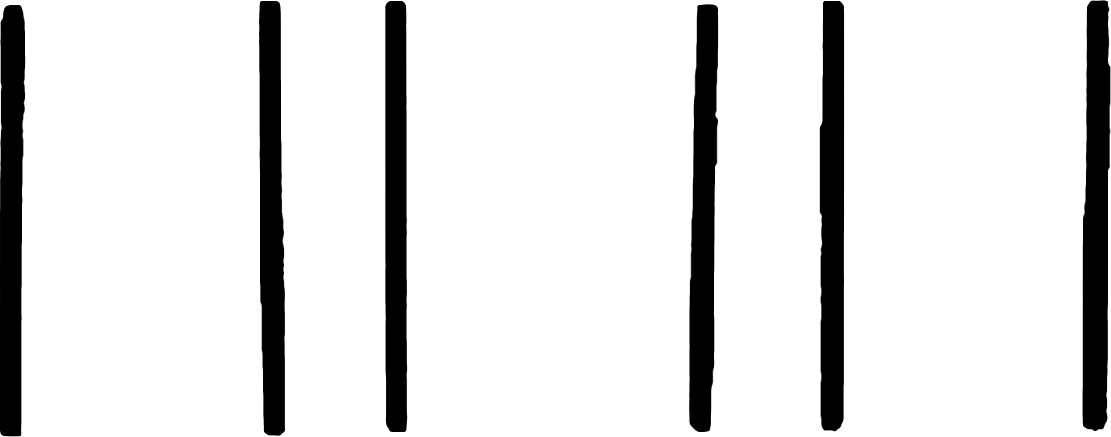
\includegraphics[width=3in]{img/strokes}\vskip 0.7em\par}} \\
are there two groups of three, or four sets of singles and pairs?\footnote{Or, much worse, are there three bracketed gaps?})

And, how does this interact with the compulsion to recognize that a derivation is legal?

Referring once again to the canard that mathematics can be explained by analogy with chess, chess is defined by rules \textbf{which depend on naive arithmetic and logic for their expression.} Moreover, mathematics is obviously not chess because mathematics is infinitary.

Could chaos in ordainment make a preposterous move legal?---or would it just cancel the system? Suppose one considers the rules of chess meaningless; or considers the claim that chess rules are meaningful to be inconsistent. Are matters then so chaotic that Kt--K6 is arguably legal as an opening move?

(Regarding chess, judgments of legality are fluid, negotiable---as they are in mathematics. Rules are altered in connection with tournament play. Also, the possible wins in chess change when very long, unintuitive games are allowed.)

\jarule

Nicholas Goodman says that it may not be true that all natural numbers are either prime or not---because for very large specific numbers the determination is too long to actually be done. So \enquote{unknowable} has to be added as a third truth-value.

But:
\begin{enumerate}[label=\arabic*), itemsep=1ex]
\item Merely adding \enquote{unknowable} as a third truth-value does not explicate Brouwer's logic---so that fails as a motivation.
\item The classical mathematician may reasonably say that it is much more convenient to idealize mathematical reality, and avoid the nuisance of the third truth-value, by imagining that all questions which extrapolate feasible questions in a homogeneous way have definite answers \enquote{known to God.} (Is that just mathematical induction?) You invent the mathematical universe this way because it is convenient or elegant.
\end{enumerate}

Can it then be guaranteed that structures which are trans-feasible and chosen for elegance will preclude $\vdash A$ and $\vdash\lnot A$? \enquote{Assuming that every question (including \enquote{infeasible} ones) has exactly one answer will not produce an inconsistency.}

Brouwer sought to prove that if the conventional classical assumption is made that \enquote{questions we cannot answer have definite answers for God,} one can get counter-examples to mandatory tenets of classical analysis. Classical mathematicians hit back by rejecting the key step in Brouwer's proof as illegal.

Goodman's objection to Brouwer is that Brouwer has a capricious attitude which itself doesn't take care to exclude inconsistency. But the same complaint is made against classical mathematics and its attitude of \enquote{Why not posit that all mathematical questions already have answers every though we don't know the answers now and may never know them?}

\jarule

The only rationale of mathematics which foundations of mathematics is prepared to defend metaphysically is formalism. (I don't mean that most twentieth-century mathematicians are formalists; I mean that Platonists such as Frege himself were not prepared to be forthright prophets of the supra-terrestrial world. \enquote{Chain of being} doctrines were expounded only by theosophists.) More narrowly, foundations of mathematics is prepared to champion only a concept of whole numbers relative to which the notion of a number's magnitude is meaningless. (Again, that doesn't mean that mathematicians don't hold far more traditional beliefs.)

It was when I offered concept art to some mathematical logicians that I ran into the real loyalties, which are atavistically traditional and theological. (Particularly when I presented \essaytitle{1966 Mathematical Studies} to Peter Ungar at Courant Institute in 1967, also when I presented it to Dennis Johnson at the Institute for Advanced Study in 1970. One may also consult the writings on foundations of mathematics by my schoolmate Nicholas Goodman.)

When one composes truly uninterpreted calculi (calculi which do not point to a naive-arithmetical interpretation)---or when one defines whole numbers which have the \enquote{wrong} magnitudes---then professional mathematicians want no part of the exercise.

\section{Bibliography}
\begin{hangparas}{2em}{1}

 Aristotle, \booktitle{Metaphysics}

 Michael Beeson, \booktitle{Foundations of Constructive Mathematics} (1985)

 Eric T. Bell, \booktitle{The Development of Mathematics} (1945)

 P. Benacerraf \& H. Putnam, eds., \booktitle{Philosophy of Mathematics} (1964)

 P. Bernays, \booktitle{Sur le platonisme} (1935)

 E.W. Beth, \papertitle{Remarks on Intuitionistic Logic,} in A. Heyting, ed., \booktitle{Constructivity in Mathematics} (1959)

 Errett Bishop \papertitle{Mathematics as a Numerical Language} in \booktitle{Intuitionism and Proof Theory}, ed. A. Kino, J. Myhill, \& R.E. Vesley (1970)

 David Bloor, \booktitle{Knowledge and Social Imagery} (1976)

 Bernard Bolzano, \booktitle{Paradoxes of the Infinite} (tr. 1950)

 L.E.J. Brouwer, \papertitle{The Rejected Parts of Brouwer's Dissertation on the Foundations of Mathematics,} \booktitle{Historica Mathematica 6} (1979)

 L.E.J. Brouwer, \booktitle{Collected Works, Vol. 1}

 George Spencer Brown, \booktitle{Laws of Form} (1979)

 Rudolf Carnap, \papertitle{The Elimination of Metaphysics Through Logical Analysis of Language,} in \booktitle{Logical Positivism}, ed. A.J. Ayer (1959)

 Rudolf Carnap, \papertitle{Pseudoproblems in Philosophy,} in \booktitle{The Logical Structure of the World} (tr. 1967)

 Rudolf Carnap, \booktitle{Logical Syntax of Language} (1937)

 Rudolf Carnap, \booktitle{Meaning and Necessity} (2nd ed., 1956)

 Felix Cleve, \booktitle{The Giants of Pre-Sophistic Greek Philosophy} (1965) B188.C55

 Richard Dedekind, \booktitle{Essays on the Theory of Numbers} (1901)

 J.J. de Iongh, \papertitle{Restricted Forms of Intuitionistic Mathematics,} in Evert Beth, ed., \booktitle{Proceedings of the Xth International Congress of Philosophy} (1949)

 Ren\'{e} Descartes, \papertitle{Rules for the Direction of the Mind,} in \booktitle{The Philosophical Writings of Descartes, Vol. I} (1985)

 Michael Dummett, \booktitle{Elements of Intuitionism} (1977), pp. 10--11

 Euclid, \booktitle{Elements} (tr. 1956, 2nd ed.)

 Paul Finsler, \papertitle{Gibt es unentscheidbare s\"{a}tze,} in \booktitle{Commentarii mathematici Helvetici} (1944), pp. 310--320, reviewed by Alonzo Church in \journaltitle{Journal of Symbolic Logic}, Vol. 11, pp. 131--132

 Gottlob Frege, \booktitle{The Foundations of Arithmetic} (tr. 1950)

 Gottlob Frege, selections from \booktitle{Grundgesetze der Arithmetik}, in \booktitle{Translations from the Philosophical Writings of Gottlob Frege} (2nd ed., 1960)

 Hans Freudenthal, \booktitle{Lincos: Design of a Language for Cosmic Intercourse} (1960)

 James Gleick, \papertitle{Machine Beats Man On Ancient Front}, \journaltitle{The New York Times}, August 26, 1986, p. C1 (about Dr. Kenneth Thompson, AT\&T Bell Laboratories, Murray Hill, New Jersey)

 Nicolas Goodman, \papertitle{Mathematics as an Objective Science}, \journaltitle{American Mathematical Monthly} (1979), pp. 540--551

 Nicolas Goodman in F. Richman, \booktitle{ed., Constructive Mathematics} (1981)

 R.L. Goodstein, \booktitle{Constructive Formalism} (1951)

 I . Grattan-Guinness, \booktitle{The Development of the Foundations of Mathematical Analysis from Euler to Riemann} (MIT, 1970)

 Emil Grosswald, \booktitle{Topics from the Theory of Numbers} (1966), pp. 27--8

 Thomas Heath, \booktitle{A History of Greek Mathematics} (1921)

 Thomas Heath, \booktitle{Mathematics in Aristotle} (1949)

 Arend Heyting, \booktitle{Intuitionism: An Introduction} (1971)

 David Hilbert, \booktitle{Foundations of Geometry}

 David Hilbert \& P. Bernays, \booktitle{Grundlagen der Mathematik} (1934-39)

 David Hilbert \& W. Ackermann, \booktitle{Principles of Mathematical Logic} (1950)

 Edmund Husserl, \booktitle{Philosophie der Arithmetik} (1891)

 Edmund Husserl, \journaltitle{G\"{o}ttinger gelehrte Anzeigen}, 1891, No. 7, p. 272 \linebreak{}
 [Husserl attacks the empty set]

 Edmund Husserl, \booktitle{The Phenomenology of Internal Time-Consciousness}, tr. James Churchill (Bloomington, 1964)

 Morris Kline, \booktitle{Mathematical Thought from Ancient to Modern Times} (1972)

 G.T. Kneebone, \booktitle{Mathematical Logic and the Foundations of Mathematics} (1963)

 Imre Lakatos, ed., \booktitle{Problems in the Philosophy of Mathematics} (1967)

 Imre Lakatos, \booktitle{Mathematics, Science, and Epistemology} (1978)

 \booktitle{Logic, Methodology, and Philosophy of Science}, ed. Nagel, Suppes, and Tarski (1962)

 Andrei A. Markov, \booktitle{Theory of Algorithms} (1961)

 Gregory Moore, \booktitle{Zermelo's Axiom of Choice} (1982)

 Jan Mycielski, \papertitle{Analysis Without Actual Infinity}, \journaltitle{Journal of Symbolic Logic}, Vol. 46, p. 625

 Edward Nelson, \booktitle{Predicative Arithmetic} (1986)

 Plato, \booktitle{Meno}

 Plato, \booktitle{Philebus}

 Plato, \booktitle{Timeaus}

 Emil Post in Martin Davis, ed., \booktitle{The Undecidable} (1964)

 Proclus, \booktitle{A Commentary on the First Book of Euclid's Elements}, tr. Glenn Morrow (1970)

 W.V.O. Quine, \booktitle{Mathematical Logic} (revised)

 W.V.O. Quine, \booktitle{Methods of Logic}

 Frank P. Ramsey, \booktitle{The Foundations of Mathematics} (1931)

 Hans Reichenbach, \booktitle{Elements of Symbolic Logic} (1947)

 Michael Resnik, \booktitle{Frege and the Philosophy of Mathematics} (1980)

 Gabriel Stolzenberg, \papertitle{Can an Inquiry into the Foundations of Mathematics Tell Us Anything Interesting about Mind?}, in \journaltitle{Psychology and Biology of Language and Thought} (1978)

 Alfred Tarski, \booktitle{Logic, Semantics, Metamathematics} (1956)

 Alfred Tarski, \papertitle{The Semantic Conception of Truth,} \journaltitle{Philosophy and Phenomenological Research 4} (1944)

 Dirk van Dalen, \booktitle{Logic and Structure} (1983)

 D. van Dantzig, \papertitle{Comments on Brouwer's Theorem on Essentially-negative Predicates}, \journaltitle{Indagationes Mathematicae}, Vol. 11, pp. 347--55

 Jean van Heijenoort, ed., \booktitle{From Frege To Godel} (1967)

 B. van Rootselaar, \papertitle{On Subjective Mathematical Assertions}, \booktitle{Intuitionism and Proof Theory}, ed. A. Kino, J. Myhill, \& R.E. Vesley (1970)

 C.F. von Weizsäcker, \booktitle{The Unity of Nature} (1980), pp. 78-9

 Stan Wagon, \booktitle{The Banach-Tarski Paradox} (1985)

 Hermann Weyl, \booktitle{Philosophy of Mathematics and Natural Science} (1949)

 Leslie A. White, \papertitle{The Locus of Mathematical Reality: An Anthropological Footnote,} in J.R. Newman, ed., \journaltitle{The World of Mathematics}, Vol. 4

 A. Whitehead and B. Russell, \booktitle{Principia Mathematica}

 Ludwig Wittgenstein, \booktitle{Wittgenstein's Lectures on the Foundations of Mathematics} (1976)

 Ludwig Wittgenstein, \booktitle{Philosophical Grammar} (1974)

Ludwig Wittgenstein, \booktitle{Remarks on the Foundations of Mathematics} (1978 ed.)
\end{hangparas}



% \chapter{The Apprehension of Plurality (1987)}

% if we end up needing to add it:
% https://henryflynt.org/studies_sci/reqmath.html

{\centering\itshape
(An instruction manual for 1987 concept art)\par}

\section{Original Stroke-Numerals}

Stroke-numerals were introduced in foundations of mathematics 
by the German mathematician David Hilbert early in the twentieth 
century. Instead of a given Arabic numeral such as `6', for example, one 
has the expression consisting of six concatenated occurrences of the 
stroke, e.g. `$||||||$'. 

To explain the use of stroke-numerals, and to provide a background 
for my innovations, some historical remarks about the philosophy 
of mathematics are necessary. Traditional mathematics had 
treated positive whole-number arithmetic as if the positive whole 
numbers (and geometrical figures also) were objective intangible 
beings. Plato is usually named as the originator of this view. Actually, 
there is a scholarly controversy over the degree to which Plato espoused 
the doctrine of Forms---over whether Aristotle's \booktitle{Metaphysics} put 
words in Plato's mouth---but that is not important for my purposes. 
For an intimation of the objective intangible reality of mathematical 
objects in Plato's own words, see the remarks about "divine" geometric 
figures in Plato's \essaytitle{Philebus.} Aristotle's \booktitle{Metaphysics}, 
1.6, says that mathematical entities 
\begin{quotation}
are intermediate, differing from things perceived in being eternal and 
unchanging, and differing from the Forms in that they exist in copies, 
whereas each Form is unique. 
\end{quotation}

For early modern philosophers such as Hume and Mill, any such 
"Platonic" view was not credible and could not be defended seriously. 
Thus, attempts were made to explain number and arithmetic in ways 
which did not require a realm of objective intangible beings. In fact, 
Hume said that arithmetic consisted of tautologies; Mill that it 
consisted of truths of experience. 

Following upon subsequent developments---the philosophical 
climate at the end of the nineteenth century, and specifically 
mathematical developments such as non-Euclidian geometry---Hilbert proposed 
that mathematics should be understood as a game played with meaningless marks. 
So, for example, arithmetic concerns nothing but formal 
terms---numerals---in a network of rules. Actually, what made arithmetic 
problematic for mathematicians was its infinitary character---as 
expressed, for example, by the principle of complete induction. Thus, 
the principal concern for Hilbert was that this formal game should not, 
as a result of being infinitary, allow the deduction of both a proposition 
and its negation, or of such a proposition as $0=1$. 

But at the same time (without delving into Hilbert's distinction 
between mathematics and metamathematics), the stroke-numerals 
replace the traditional answer to the question of what a number is. The 
stroke-numeral '||||||' is a concrete semantics for the sign `6', and at the 
same time can serve as a sign in place of `6'. The problem of positive 
whole numbers as abstract beings is supposedly avoided by inventing 
e.g. a number-sign, a numeral, for six, which is identically a concrete 
semantics for six. Let me elaborate a little further. A string of six copies 
of a token having no internal structure is used as the numeral `6', the 
sign for six. Thus the numeral is itself a collection which supposedly 
demands a count of six, thereby showing its meaning. Hans Freudenthal 
calls this device an "ostensive numeral." 

So traditionally, there is a question as to what domain of beings 
the propositions of arithmetic refer to, a question as to what the 
referents of number-words are. \emph{Correlative to this, mathematicians' 
intentions require numerous presuppositions about content, and 
require extensive competancies---which the rationalizations for math- 
ematics today are unable to acknowledge, much less to defend.}

For example, if mathematics rests on concrete signs, as Hilbert 
proposed, then, since concrete signs are objects of perception, the 
reliability of mathematics would depend on the reliability of percep- 
tion. Given the script numeral 
{\plainbreak{1}\centering\includegraphics[width=1in]{img/oneortwo}\plainbreak{1}}
which is ambiguous between one and two, conventional mathematics 
would have to guarantee the exclusion of any such ambiguity as this. 
Yet foundations of mathematics excludes perception and the reliability 
of concrete signs as topics---much as Plato divorced mathematics from 
these topics. (Roughly, modern mathematicians would say that reliability 
of concrete signs does not interact with any advanced mathematical 
results. So this precondition can simply be transferred from the requisites 
of cognition in general. But it would not be sincere for Hilbert to 
give this answer. Moreover, my purpose is to investigate the possibility 
of reconstructing our intuitions of quantity beyond the limits of the 
present culture. In this connection, I need to activate the role of 
perception of signs.) 

But the most characteristic repressed presuppositions of mathematics 
run in the opposite, supra-terrestrial direction. Mathematicians' 
intentions require a realm of abstract beings. Again, it is academically 
taboo today to expose such presuppositions.
\footnote{G\"{o}del and Quine admit the need to assume the non-spatial, abstract 
existence of classes. But they cannot elaborate this admission; they cannot 
provide a supporting metaphysics.} But to recur to the 
purpose of this investigation, concept art is about reconstructing our 
intuitions of quantity beyond the limits of the present culture. This 
project demands an account of these repressed presuppositions. To 
compile such an account is a substantial task; I focus on it ina collateral 
manuscript entitled "The Repressed Content-Requirements of Math- 
ematics." To uncover the repressed presuppositions, a combination of 
approaches is required.\footnote{One anthroplogist has written about \enquote{the locus of 
mathematical reality}---but, being an academic, he merely reproduces a stock answer outside 
his field (namely that the shape of mathematics is dictated by the physiology of 
the brain).} I will not dwell further on the matter here---
but a suitable sample of my results is the section "The Reality-Character 
of Pure Whole Numbers and Euclidian Figures" in \emph{The Repressed Content-Requirements.}

Returning to the original stroke-numerals, they were meant 
(among other things) to be part of an attempt to explain arithmetic 
without requiring numbers as abstract beings. They were meant as 
signs, for numbers, which are identically their own concrete semantics. 
Whether I think Hilbert succeeded in dispensing with abstract entities is 
not the point here. I am interested in how far the exercise of positing 
stroke-numerals as primitives can be elaborated. My notions of the 
original stroke-numerals are adapted from Hilbert, Weyl, Markov, 
Kneebone, and Freudenthal. For example, how does one test two 
stroke-numerals for equality? To give the answer that "you count the 
strokes, first in one numeral and then in the other," is not in the spirit of 
the exercise. For if that is the answer, then that means that you have a 
competency, "counting," which must remain a complete mystery to 
foundations of mathematics. What one wants to say, rather, is that you 
test equality of stroke-numerals by "cross-tallying": by e.g. deleting 
strokes alternately from the two numerals and finding if there is a 
remainder from one of the numerals. This is also the test of whether one 
numeral precedes the other. So, now, given an adult mastery of quality 
and abstraction, you can identify stroke-numerals without being able 
to "count." 

In the same vein, you add two stroke-numerals by copying the 
second to the right of the first. You subtract a shorter numeral from a 
longer numeral by using the shorter numeral to tally deletion of strokes 
from the longer numeral. You multiply two stroke-numerals by copying the second as many times as there are strokes in the first: that is, by 
using the strokes of the first to tally the copying of the second numeral. 

To say that all this is superfluous, because we already acquired 
these "skills" as a child, misses the point. The child does not face the 
question, posed in the Western tradition, of whether we can avoid 
positing whole numbers as abstract beings. To weaken the requirements 
of arithmetic to the point that somebody with an adult mastery 
of quality and abstraction can do feasible arithmetic "blindly"---i.e. 
without being able to "count," and without being able to see number-names 
('five', 'seven', etc.) in concrete pluralities---is a notable exercise, 
one that correlates culturally with positivism and with the machine age. 

To reiterate, the stroke-numeral is meant to replace numbers as 
abstract beings by providing number-signs which are their own concrete 
semantics. Freudenthal said that we should communicate positive 
whole numbers to alien species by broadcasting stroke-numerals to 
them (in the form of time-series of beeps). Still, Freudenthal said that 
the aliens would have to resemble us psychologically to get the point.\footnote{\booktitle{Lincos}, pp. 14--15.} 

When Hilbert first announced stroke-numerals, certain difficulties 
were pointed out immediately. It is not feasible to write the 
stroke-numerals for very large integers. (And yet, if it is feasible to write the 
stroke-numeral for the integer n, then there is no apparent reason why 
it would not also be feasible to write the stroke-numeral for n+1. So 
stroke-numerals are closed under succession, and yet are contained in a
finite segment of the classical natural number series.) Moreover, large 
feasible stroke-numerals, such as that for 10,001, are not surveyable. 

But this is not a study of metamathematical stroke-numerals. And 
I do not wish to go into Hilbert's question of the consistency of 
arithmetic as an infinitary game here; "The Repressed Content-Requirements" 
will have more to say on the consistency question. The 
purpose of this manual, and of the artworks which it accompanies, is to 
establish apprehensions of plurality beyond the limits of traditional 
civilizations (beyond the limits of Freudenthal's "us"). Moreover, these 
apprehensions of plurality are meant to violate the repressed presuppo- 
sitions of mathematics. I refer back to original stroke-numerals because 
certain devices which I will use in assembling my novelties cannot be 
supposed to be intuitively comprehensible---certainly not to the 
traditionally-indoctrinated reader---and will more likely be understood 
if I mention that they are adaptations of features of original stroke- 
numerals. Let me mention one point right away. In our culture, we 
usually see numerals as positional notations---e.g. 111 is decimal 
$1\times 10^2+1\times 10^1+1$ or binary $1\times 2^2+1\times 2^1+1$. But stroke-numerals 
are not a positional notation (except trivially for base 1). Likewise, my 
novelties will not be positional notations; I will even nullify the 
reference to base 1. (Only much later in my investigations, when broad 
scope becomes important, will I use positional notation.) So the 
foregoing introduction to stroke-numerals has only the purpose of 
motivating my novelties. And references to the academic canon are given 
only for completeness. They cannot be norms for what I am "permitted" to posit. 

\section{Simple Necker-Cube Numerals}

In my stroke-numerals, the printed figure, instead of being a 
stroke, is a Necker cube. (Refer to the attached reproduction, "Stroke- 
Numeral.") A Necker cube is a two-dimensional representation of a 
cubical frame, formed without foreshortening so that its perspective is 
perceptually equivocal or multistable. The Necker cube can be seen as 
flat, as slanting down from a central facet like a gem, etc.; but for the 
moment I am exclusively concerned with the two easiest variants in 
which it is seen as an ordinary cube, either projecting up toward the 
front or down toward the front. 

{\center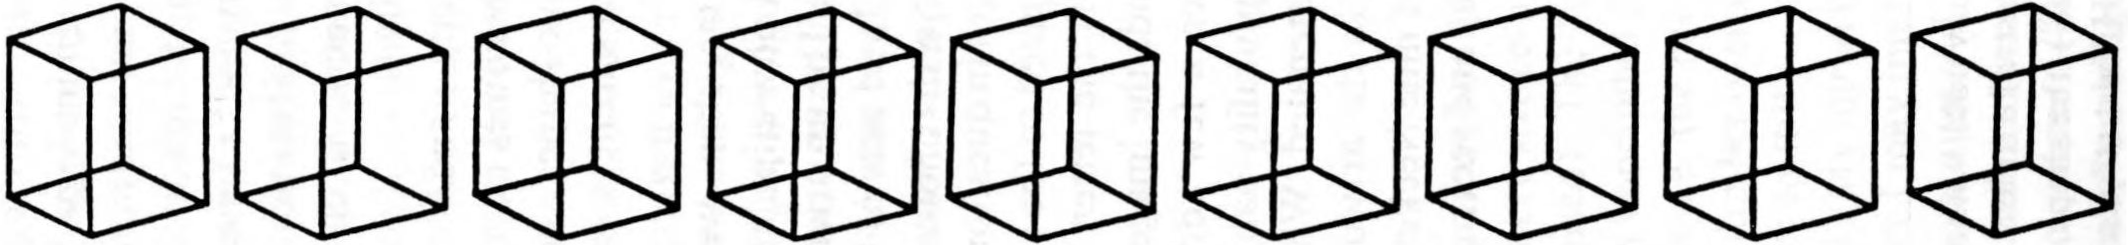
\includegraphics[width=4in]{img/neckercube}\plainbreak{2}
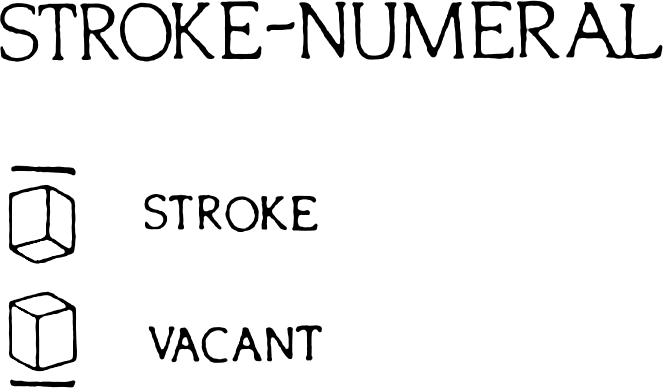
\includegraphics[width=2in]{img/neckerkey}\par}

Since I will use perceptually multistable figures as notations, I 
need a terminology for distinctions which do not arise relative to 
conventional notation. I call the ink-shape on paper a \term{figure}. I call the 
stable apparition which one sees in a moment---which has imputed 
perspective---the \term{image}.\footnote{I may note, without wanting to be precious, that a bar does not count as a Hilbert stroke unless it is vertical relative to its reader.}
As you gaze at the figure, the image changes 
from one orientation to the other, according to intricate subjective 
circumstances. It changes spontaneously; also, you can change it 
voluntarily. 

Strictly---and very importantly---it is the image which in this 
context becomes the notation. Thus, I will work with notations which 
are not ink-shapes and are not on a page. They arise as active interactions 
of awareness with an "external" or "material" print-shape or 
object. 

So far, then, we have images---partly subjective, pseudo-solid 
shapes. I now stipulate an alphabetic role for the two orientations in 
question. The up orientation is a \term{stroke}; the down orientation is called 
"\term{vacant}," and acts as the proofreaders' symbol $\closure$, meaning "close up space." 
(So that "vacant" is not "even" an alphabetic space.) Now the 
two images in question are \term{signs}. The transition from image to sign can 
be analogized to the stipulation that circles of a certain size are (occurances 
of) the letter "o."\footnote{And---the shape, bar, positioned vertically relative to its reader, is the symbol, Hilbert stroke.} I may say that one sees the image; one 
apprehends the image as sign. 

When a few additional explanations are made, then the signs 
become plurality-names or "numerals." First, figures, Necker cubes, 
are concatenated. When this is done, a display results. So the 
stroke-numeral in the artwork, as an assembly of marks on a surface, is a 
display of nine Necker cubes. An image-row occurs when one looks at 
the display and sees nine subjectively oriented cubes, for just so long as 
the apparition is stable (no cube reverses orientation). I chose nine 
Necker cubes as an extreme limit of what one can apprehend in a fixed 
field of vision. (So one must view the painting from several meters 
away, at least.) The reader is encouraged to make shorter displays for 
practice. Incidentally, if one printed a stroke-numeral so long that one 
could only apprehend it serially, by shifting one's visual field, it would 
be doubtful that it was well-defined. (Or it would incorporate a feature 
which I do not provide for.) The universe of pluralities which can be 
represented by these stroke-numerals is "small." My first goal is to 
establish "subjectified" stroke-numerals at all. They don't need to be 
large. 

The concatenated signs which you apprehend in a moment of 
looking at the display are now apprehended or judged as a 
plurality-name, a numeral. At the level where you apprehend signs (which, 
remember, are alphabetized, partly subjective images, not figures), the 
apparition is disambiguated. Thus I can explain this step of judging the 
signs as plurality-names by using fixed notation. For nine Necker cubes 
with the assigned syntactical role, you might apprehend such 
permutations of signs as 
\begin{enumerate}[label=\alpha*.]
	\item $|\closure\closure||\closure\closure\closure|$
	\item $|\closure\closure\closure\closure\closure|||$
	\item $||||\closure\closure\closure\closure\closure$
	\item $||||\closure\closure\closure\closure|$
	\item $\closure\closure\closure\closure\closure\closure\closure\closure\closure$
\end{enumerate}

My Necker-cube stroke-numerals are something new; but (a)--(e) are 
not---they are just a redundant version of Hilbert stroke-numerals 
(which nullifies the base 1 reference as I promised). The "close up 
space" signs function as stated; and the numeral concluded from the 
expression corresponds to the number of strokes; i.e. the net result is 
the Hilbert stroke-numeral having the presented number of strokes. So 
(a) and (b) and (c) all amount to $|||$. (d) amounts to $|||||$.

As for (e), it has the alphabetic role of a blank. My initial interpretation 
of this blank is "no numeral present." Later I may interpret the 
blank as "zero," so that every possibility will be a numeral. Let me 
explain further. Even when I will interpret the blank as "zero." it will 
not come about from having nine zeros mapped to one zero (like a sum 
of zeros). (e) has nine occurrences of "close up space," making a blank. 
There is always only one way of getting "blank." (A two-place display 
allows two ways of getting "one" and one way of getting "two"; etc.) 
The notation is not positional. It is immaterial whether one "focuses" 
starting at the left or at the right. 

Relative to the heuristic numerals (a)--(e), you may judge the 
intended numerals by counting strokes, using your naive competency 
in counting. (It is also possible to use such numerals as (a)--(e) "blindly" 
as explained earlier. This might mean that there would be no recognition 
of particular numbers as gestalts; identity of numbers would be
handled entirely by cross-tallying.) The Necker-cube numerals, however, 
pertain to a realm which is in flux because it is coupled to 
subjectivity. My numerals provide plurality-names and models of that 
realm. Thus, the issue of what you do when you conclude a numeral 
from a sign in perception is not simple. \emph{We have to consider different 
hermeneutics for the numerals---and the ramifications of those hermeneutics.}
Here we begin to get a perspective of the mutability which my 
devices render manageable. 

For one thing, given a (stable) image-row, and thus a sign-row, you 
can indeed use your naive arithmetical competency to count strokes, 
and so conclude the appropriate numeral. This is \term{bicultural hermeneutic}, 
because you are using the old numbers to read a new notation for 
which they were not intended. We use the same traditional counting, of 
course, to speak of the number of figures in a display. 

(This prescription of a hermeneutic is not entirely straightforward. 
The competency called counting is required in traditional mathematics. 
But such counting is already paradoxical "phenomenologically." I 
explain this in the section called "Phenomenology of Counting" in \essaytitle{The 
Repressed Content-Requirements}. As for the Necker-cube numerals, 
the elements counted are not intended in a way which supports the 
being of numbers as eternally self-identical. So the Necker-cube 
numerals might resonate with the phenomenological paradoxes of 
ordinary counting. The meaning of ordinary numbering, invoked in 
this context, might begin to dissolve. But I mention this only to hint at 
later elaborations. At this stage, it is proper to recall one's inculcated 
school-counting; and to suppose that e.g. the number of figures in a 
display is fixed in the ordinary way.) 

Then, there is the \term{ostensive hermeneutic}. Recall that I explained 
Hilbert stroke-numerals as signs which identically provide a concrete 
semantics for themselves; and as an attempt to do arithmetic without 
assuming that one already possesses arithmetic in the form of competency 
in counting, or of seeing number-names in pluralities. My 
intention was to prepare the reader for features to be explained now. 
On the other hand, at present we drop the notion of handling identity of 
numerals by cross-tallying.\footnote{Because this notion corresponds to a situation in which we are unable to appraise image-rows as numerals, as gestalts.}
For the ostensive hermeneutic, it is crucial 
that the display is short enough to be apprehended in a fixed field of 
vision. 

With respect to short Hilbert numerals, I ask that when you see 
e.g. 

$$||$$

marked ona wall, you grasp it asa sign for a definite plurality, without 
mediation---without translating to the word "two." A similar intention 
is involved in recognizing 
$$\sout{||||}$$
as a definite plurality, as a gestalt, without translating to "five." 

Now I ask you to apply this sort of hermeneutic to Necker-cube 
stroke-numerals. I ask you to grasp the sign-row as a numeral, as a 
gestalt. (Without using ordinary counting to call off the strokes.) Fora 
two-place display, you are to take such images as 

\newcommand{\neckup}{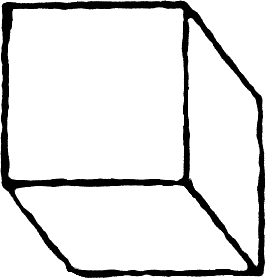
\includegraphics[width=1in]{img/neckerup}}
\newcommand{\neckdown}{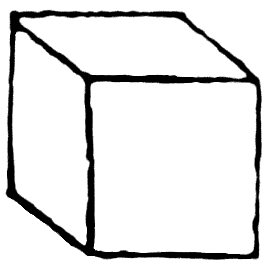
\includegraphics[width=1in]{img/neckerdown}}

{\centering\neckup\neckdown\par}
and
{\centering\neckup\neckup\par}
as plurality-names without translating into English words. (Similarly 

{\centering\neckdown\neckdown\par}

in the case where I choose to read "blank" as "zero.") Perhaps it is 
necessary to spend considerable time with this new symbolism before 
recognition is achieved. Again, I encourage the reader to make short 
displays for practice. I have set a display of nine figures as the upper 
limit for which it might be possible to learn to grasp every sign-row as a 
numeral, as a gestalt. 

The circumstance that the apprehended numeral may be different 
the next moment is not a mistake; the apprehended numeral is supposed 
to be in flux. So when you see image-rows, you take them as 
identical signs/semantics for the appearing pluralities. 

But who wants such numerals---where are there any phenomena 
for them to count? For one thing, they count the very image-rows which 
constitute them. The realm of these image-rows is a realm of subjective 
flux: its plurality is authentically represented by my numerals, and 
cannot be authentically represented by traditional arithmetic. 

A further remark which may be helpful is that here numerals arise 
only visually. So far, my numerals have no phonic or audio equivalent. 
(Whereas Freudenthal in effect posited an audio version of Hilbert 
numerals, using beeps.) 

To repeat, by the "ostensive hermeneutic" I mean grasping the 
sign-row, without mediation, as a numeral. But there is, as well, the 
point that the Necker-cube numerals are \term{ostensive numerals}. That is, 
the (momentary) numeral for six would in fact be an image-row with 
just six occurrences of the image "upward cube." (Compare e.g. 
$|||\closure\closure||\closure|$) The numeral is a collection in which only the "copies" of 
"upward cube" contribute positively, so to speak; and these copies 
demand a count of six (bicuturally). This feature needs to be clear, 
because later I will introduce numerals for which it does not hold. 

Let me add another proviso concerning the ostensive hermeneutic 
which will be important later. I will illustrate the feature in question 
with an example which, however, is only an analogy. Referring to 
Arabic decimal-positional numerals, you can appraise the number-name of 
$$1001$$
(comma omitted) immediately. But consider 
$$786493015201483492147$$
Here you cannot appraise the number-name without mediation. That 
is, if you are asked to read the number aloud, you don't know whether 
to begin with "seven" or "seventy-eight" or "seven hundred eighty-six." 
Lacking commas, you have to group this expression from the right, in 
triples, to find what to call it. An act of analysis is required. 

In the case of Necker-cube numerals and the ostensive hermeneutic, 
I don't want you to see traditional number-names in the pluralities. 
However, I ask you to grasp a sign-row as a numeral, as a gestalt. I now 
add that the gestalt appraisal is definitive. I rule out appraising image-rows 
analytically (by procedures analogous to mentally grouping an 
Arabic number in triples). (I established a display of nine figures as the 
upper limit to support this.) 

The need for this proviso will be obscure now. It prepares for a 
later device in which, even for short displays, gestalt appraisal and 
appraisal by analysis give different answers, either of which could be 
made binding. 

\breatk

The bicultural hermeneutic is applied, in effect, in my uninterpreted 
calculus \textsc{"Derivation,"} which serves as a simplified analogue of 
my early concept art piece \textsc{"Illusions."} (Refer to the reproductions on 
the next four pages.) Strictly, though, "Derivation" does not concern a 
Necker-cube stroke-numeral. The individual figures are not Necker 
cubes, but "Wedberg cubes," formed with some foreshortening to make 
one of the two orientations more likely to be seen than the other. What 
is of interest is not apprehension of image-rows as numerals, but rather 
appraisal of lengths of the image-rows via ordinary counting. As for the 
lessons of this piece, a few simple observations are made in the piece's 
instructions. But to pursue the topic of concept art as uninterpreted 
calculi, and derive substantial lessons from it, will require an entire 
further study---taking off from earlier writings on post-formalism and 
uncanny calculi, and from my current writings collateral to this essay. 


1987 Concept Art --- Henry Flynt 
"DERIVATION" (August 1987 corrected version) 


Purpose: To provide a simplified analogue of my 1961 concept art piece "'IIlusions'' which is 
discrete and non-''warping.''* Thereby certain features of "'Illusions'' become more 
clearly discernible. 


Given a perceptually multistable figure, the ""Wedberg cube," which can be seen in two 
orientations: as a cube; as a prism (trapezohedron.) 

Call what is seen at an instant an /mage. 

Nine figures are concatenated to form the display. 


An element is an image of the display for as long as that image remains constant (Thus, 
elements include: the image from the first instant of a viewing until the image first 
changes; an image for the duration between two changes; the image from the last 
change you see in a viewing until the end of the viewing.) 


The /ength of an element equals the number of prisms seen. Lengths from O through nine 
are possible. Two different elements can have the same length. Length of element X 
is written /(X). 


Elements are seen in temporal order in the lived time of the spectator. | refer to this order by 
words with prefix 'T'. T-first; T-next; etc. 


Element Y succeeds element X if and only if 
i) (X) = KY), and Y is T-next after X of all elements with this length; or 
ii) ¥ is the T-earliest element you ever see with length /(X) + 1. 
Note that (ii) permits Y to be T-earlier than X: the relationship is rather artificial. 


The initial element A is the T-first element. (/(A) may be greater than O; but it is likely to be O 
because the figure is biased.) 


The conclusion C is the T-earliest element of length 9 (exclusive of Ain the unlikely case in 
which /(A) = 9). 


A derivation is a series of elements in lived time which contains A and C and in which every 
element but A succeeds some other element. 


Discussion 

To believe that you have seen a derivation, you need to keep track that you see each 
possible length, and to force yourself to see lengths which do not occur spontane- 
ously. 


You may know that you have seen a derivation, without being able to identify in memory the 
particular successions. 


"Derivation" is not isomorphic to "Illusions" for a number of reasons. ''Illusions" doesn't 
require you to see individually every possible ratio between the T-first ratio and unity. 
"Illusions" allows an element to succeed itself. The version of 'Derivation' pres- 
ented here is a compromise between mimicking "'Illusions"' and avoiding a trivial or 
cluttered structure. Any change such as allowing elements to succeed themselves 
would require several definitions to be modified accordingly. 


*In "Illusions," psychic coercion, which may be called "false seeing" or "warping," is 
recommended to make yourself see the ration as unity. In ''Derivation," this warping is not 
necessary; all that may be needed is that you see certain lengths willfully. 


ABABA AAS 


Concept Art Version of Mathematics System 3/26/6l(6/19/61) 

An "element"is the facing page (with the figure on it) so long 
as the apparent, perceived, ratio of the length of the vertical 
line to that of the horizontal line (the element's "associated 
ratio") does not change. 

A "selection sequence" is asequence of elements of which the 
first is the one having the greatest associated ratio, and 
each of the others has the associated ratio next smallerthan 
that of the preceding one. (To decrease the ratio, come to 
see the vertical line as shorter, relative to the horizontal 
line, one might try measuring the lines with a ruler to con- 
vince oneself that the vertical one is not longer than the 
other, and then trying to see the lines as equal in length; 
constructing similar figures with a variety of real (measured) 
ratios and practicing judging these ratios; and so forth.) 
(Observe that the order of elements in a selection sequence 
may not be the order in which one sees them.] 


An elaboration of "Stroke-Numeral" should be mentioned here, 
the piece called "an Impossible Constancy." (Refer to the facing page.) 
As written, this piece presupposes the bicultural hermeneutic, and that 
is probably the way it should be formulated. The point of this piece, 
paradoxically, is that one seeks to annul the flux designed into the 
apprehended numeral. Viewing of the Necker-cube numeral is placed 
in the context of a lived experience which is interconfirmationally 
weak: namely, memory of past moments within a dream (a single 
dream). Presumably, appraisals of the numeral at different times could 
come out the same because evidence to the contrary does not survive. 
So inconstancy passes as constancy. Either hermeneutic can be 
employed; but when I explained the hermetic hermeneutic, I encour- 
aged you to follow the flux. Here you wouldn't do that---you wouldn't 
stare at the display over a retentional interval. 


As for the concept of equality with regard to Necker-cube numerals, 
what can be said about it at this point? We have equality of numbers of 
figures in displays, by ordinary counting. We have two hermeneutics 
for identifying an apprehended numeral. In the course of expounding 
them, I expounded equivalence of different permutations of "stroke" 
and "vacant." Nevertheless, given that, for example, a display of two 
figures can momentarily count the numeral apprehended from a dis- 
play of three figures,* we are in unexplored territory. Cross-tallying, 
suitable for judging equality of Hilbert numerals, seems maladapted to 
Necker-cube numerals; in fact, I dismissed it when introducing the 
ostensive hermeneutic. 

If the "impossible constancy" from the paragraph before last were 
manageable, then one might consider restricting the ultimate definition 
of equality to impossible constancies. That is, with respect to a single 
display, if one wanted to investigate the intention of constancy (self- 
equivalence of the apprehended numeral), one might start with the 
impossible constancy. Appraisals of a given display become constant 
(the numeral becomes self-equivalent) in the dream. Then two displays 
which are copies might become constantly equivalent to each other, in 
the dream. 

Such is a possibility. To elaborate the basics and give an incisive 
notion of equality is really an open problem, though. Other avenues 
might require additional devices such as the use of figures with distinc- 
tions of appearance. 


*that it is not assured that copies of a numeral will be apprehended or 
appraised correlatively 


1987 Concept Art --- Henry Flynt 
Necker-Cube Stroke-Numeral: AN IMPOSSIBLE CONSTANCY 


The purpose of this treatment is to say how a Necker-cube stroke numeral may be 
judged (from the standpoint of private subjectivity) to have the same value at different 
times; even though the conventional belief-system says that the value is likely to change 
frequently. 


This is accomplished by selecting a juncture in an available mode of illusion, namely 
dreaming, which annuls any distinction between an objective circumstance, and the 
circumstance which exists according to your subjective judgment. In the first instance, | 
don't ask you to change your epistemology. Instead, to repeat, | select an available juncture 
in lived experience at which the conventional epistomology gets collapsed. 


You have to occupy yourself with the stroke-numeral to the point that you induce 
yourself to dream about it. 

When, in apprehending a stroke-numeral, you "judge" the value of the numeral, the 
number, this refers to the image you see and to the number-word which you may conclude 
from the image. 

Suppose that in a single dreamed episode, you judge the value of the numeral at two 
different moments. Suppose that at the second moment, you do not register any discre- 
pancy between the value at the second moment and what the value was at the first 
moment. Then you are permitted to disregard fallibility of memory, and to conclude that the 
values were the same at both moments: because if your memory has changed the past, it 
has done so tracelessly. A tracelessly-altered past may be accepted as the genuine past. 


Refinements. The foregoing dream-construct may be "'lifted" to waking experience, as 
per the lengthy explanations in ""An Epistemic Calculus."' Now you are asked to alter your 
epistemology, selectively to suspend a norm of realism. 

Now that we are concerned with waking experience, a supporting refinement is 
possible. Suppose | make an expectation (which may be unverbalized) that the value of the 
numeral at a future moment will be the same that it is now. This expectation cannot be 
proved false, if: the undetermined time-reference 'future moment" is applied only at those 
later moments when the value is the same as at the moment the expectation was made. 
(Any later moment when the value is not the same is set aside as not pertinent, or forgotten 
at still later moments when the value is the same.) 


As a postscript, there is another respect in which testing a fact requires trust in a 
comparable fact. Suppose | make a verbalized expectation that the value of the numeral in 
the future will be the same as at present. Then to test this expectation in the future depends 
on my memory of my verbalization. My expectation cannot be belied unless | have a sound 

"memory that the number | verbalized in my expectation is different from the number | 
conclude from the image now. 


HT. Inconsistently-Valued Numerals 


As the "Wedberg cube" illustrates, a cubical frame can be formed 
in different ways, altering the likelihood that one or another image is 
seen. With respect to the initial uses of the Necker-cube stroke-numeral 
a figure is wanted which lends itself to the image of a cube projecting 
up, or of a cube projecting down, with an approximately equal likeli- 
hood for the two images---and which makes other images unlikely. 
Now let a Necker cube be drawn large, with heavy line-segments, with 
all segments equally long, with rhomboid front and back faces; and 
display it below eye level. 


As you look for the up and down orientations, there should be 
moments when paradoxically you see the figure taking on both of these 
mutually-exclusive orientations at once---yielding an apparition which 
is a logical/ geometric impossibility. The sense-content in this case is 
dizzying. 

That we have perceptions of the logically impossible when we 
suffer illusions has been mentioned by academic authors. (Negative 
afterimages of motion---the waterfall illusion.) Evidently, though, these 
phenomenaare so distasteful to sciences which are still firmly Aristote- 
lian that the relations of perception, habituation, language, and logic 
manifested in these phenomena have never been assessed academically. 
For me to treat the paradoxical image thoroughly here would be too 
much of a digression from our subject, the apprehension of plurality. 
However, a sketchy treatment of the features of the impossible image is 
necessary here. 

To begin with, the paradoxical image of the Necker cube is not the 
same phenomenon as the "impossible figures" shown in visual percep- 
tion textbooks. The latter figures employ "puns" in perspective coding 
such that parts of a figure are unambiguous, but the entire figure 


cannot be grasped as a gestalt coherently. Then, the paradoxical Necker- 
cube image is not an inconsistently oriented object (as the reader may 
have noted). It is an apparitional depiction of an inconsistently oriented 
object. But this is itself remarkable. For since a dually-oriented cube (in 
Euclidean 3-space) is self-contradictory by geometric standards, a 
picture of it amounts to a non-vacuous semantics for an inconsistency. 
Another way of saying the same thing is that the paradoxically- 
oriented image is real as an apparition. 

If one is serious about wanting a "logic of contradictions"---a logic 
which admits inconsistencies, without a void semantics and without 
entailing everything---then one will not attempt to get it by a contorted 
weakening of received academic logic. One will start from a concrete 
phenomenon which demands a logic of contradictions for its authentic 
representation---and will let the contours of the phenomenon shape the 
logic. 

In this connection, the paradoxically-oriented Necker-cube image 
provides a lesson which I must explain here. Consider states or proper- 
ties which are mutually exclusive, such as "married" and "bachelor." 
Their conjunction---in English, the compound noun "married 
bachelor"---is inconsistent.* On the other hand, the joint denial 
"unmarried nonbachelor" is perfectly consistent and is satisfied by 
nonpersons: a table is an unmarried nonbachelor. "Married" and 
"bachelor" are mutually exclusive, but not exhaustive, properties. Only 
when the domain of possibility, or intensional domain, is restricted to 
persons, so "married" and "bachelor" become exhaustive properties. ** 
Then, by classical logic, "married bachelor" and "unmarried nonbache- 
lor" both have the same semantics: they are both inconsistent, and thus 
vacuous, and thus indistinguishable. For exhaustive opposites, joint 
affirmation and joint denial are identically vacuous. 

But the paradoxically-oriented Necker-cube image provides a 
concrete phenomenon which combines mutually exclusive states---as 
an apparition. We can ascertain whether a concrete case behaves as the 
tenets of logic prescribe. As I have said, various images can be seen ina 
Necker cube, including a flat image. Thus, the "up" and "down" cubes 


*If I must show that it is academically permitted to posit notions such as 
these, then let me mention that Jan Mycielski calls "triangular circle" incon- 
sistent in The Journal of Symbolic logic, Vol. 46, p. 625. 

**] invoke this device so that I may proceed to the main point quickly. If it 
is felt to be too artificial, perhaps it can be eliminated later. 


are analogous to "married" and "bachelor" in that they are not exhaus- 
tive of a domain unless the domain is produced by restriction. Then 
"neither up nor down" is made inconsistent. (It is very helpful if you 
haven't learned to see any stable images other than "up" and "down.") 
The great lesson here is that given "both up and down" and "neither up 
nor down" as inconsistent, their concrete reference is quite different. To 
see a cube which manifests both orientations at the same time is one 
paradoxical condition, which we know how to realize. To see a cube 
which has no orientation (absence of "stroke" and absence of "vacant" 
both) would be a different paradoxical condition, which we do not 
know how to realize and which may not be realizable from the Necker- 
cube figure. I don't claim that this is fully worked out; but it intimates a 
violation of classical logic so important that I had to mention it. When 
concept art reaches the level of reconstructing our inferential intuitions 
as well as our quantitative intuitions, such anomalies as these will surely 
be important. 

Referring back to the Necker cube of page 210, let us now intend it 
as a stroke-numeral (display of one figure). Let me modify the previous 
assignments and stipulate that "blank" means "zero," rather than "no 
numeral present." (It is more convenient if every sign yields a numeral.) 
When you see the paradoxical image, you are genuinely seeing "a" 
numeral which is the simultaneous presence of two mutually exclusive 
numerals "one" and "zero" ---because it is the simultaneous presence of 
images which are mutually exclusive geometrically.*** 

It's not the same thing as 


| 


---because these are merely ambiguous scripts. In the Necker-cube case, 
two determinate images which by logic preclude each other are present 
at once; and as these images are different numerals, we have a genuine 


---or as an alternative, 


*For brevity, I may compress the three levels image, sign, numeral in 
exposition. 


inconsistently-valued numeral. 

This situation changes features of the Necker-cube numerals in 
important ways, however. Lessons from above become crucial. We 
transfer the ostensive hermeneutic to the new situation, and find an 
inconsistent-valued numeral. But this is no longer an ostensive 
numeral. We have a name which is one and zero simultaneously, but 
this is because of the impossible shape (orientation) of the notation- 
token. What we do not have is a collection of images of a single kind 
(the stroke) which paradoxically requires a count of one and a count of 
zero. "Stroke" is positively present, while "vacant" is positively present 
in the same place. We will find that a display with two figures can be 
inconsistent as zero and two; but it is not an ostensive numeral, because 
the number of strokes present is two uniquely.* Here the numerals are 
not identically their semantics: for the anomaly is not an anomaly of 
counting. The ambiguous script numeral is a proper analogy in this 
respect. To give an anomaly of counting which serves as a concrete 
semantics for the inconsistently-valued numerals, I will turn to an 
entirely different modality. 

From work with the paradoxical image, we learn that the Necker 
cube allows some apprehensions which are not as commonas others--- 
but which can be fostered by the way the figure is made and by 
indicating what is to be seen. These rare apprehensions then become 
intersubjectively determinate. If one observes Necker-cube displays for 
a long time, one may well observe subtle, transient effects. For exam- 
ple, you might see the "up" and "down" orientations at the same time, 
but see one as dominating the other. In fact, there are too many such 
effects and their interpersonal replicability is dubious. If we accepted 
such effects as determining numerals, the interpersonal replicability of 
the symbols would be eroded. Also the concrete definiteness of my 
anomalous, paradoxical effects would be eroded. So I must stipulate 
that every subtle transient effect which I do not acknowledge explicitly 
is not definitive, and is unwanted, when the display is intended as a 
symbolism. 

Let me continue the explanation, for the inconsistently-valued 


*Referring to my "person-world analysis" and to the dichotomy of 
Paradigm | and Paradigm 2 expounded in "Personhood III," this token which 
is two mutually exclusive numerals because its shape is inconsistent is outside 
that dichotomy: because established signs acquire a complication which is 
more or less self-explanatory, but the meanings do not follow suit. 


numerals, for displays of more than one figure. When the display 
consists of two Necker cubes, and the paradoxical images are admitted, 
what are the variations? In the first place, one figure might be seen (ina 
moment) as a paradoxical image and the other as a unary image. 
Actually, if it is important to obtain this variant, we can compel it, by 
drawing one of the cubes in a way which hampers the double image. 
(Thin lines, square front and back faces, the four side segments much 
shorter than the front and back segments.) Then we stipulate that the 
differently-formed cubes continue to have the same assigned interpre- 
tation. 


Reading the two-figure display, then, the paradoxical and unary 
images concatenate so that the resulting numeral is in one case one and 
two at the same time; and in the other case zero and one at the same 
time. Of course, it is only ina moment that either of these two cases will 
be realized. At other moments, one may have only unary images, so 
that the numeral is noncontradictorily zero, one, or two as the case may 
be. (If it is important to know that we can obtain a numeral which is 
both one and two at the same time without using dissimilar figures, 
then, of course, we can use a single figure and redefine the signs as "one" 
and "two.") 

Now let us consider a display of two copies of the cube which lends 
itself to the paradoxical image. Suppose that two paradoxical images 
are seen; what is the numeral? Here is where I need the proviso which I 
introduced earlier. Every sign-row is capable of being grasped as a 
numeral, as a gestalt; and the appraisal of image-rows as numerals, 
analytically, is ruled out. Let me explain how this proviso applies when 
two paradoxical images are seen. 

Indeed, let me begin with the case of a pair of ambiguous 


script-numerals: ] ] 


When these numerals are formed as exact copies, and I appraise the 
expression as a numeral, as a gestalt, then I see 11 or I see 22. ("Conca- 
tenating in parallel") I do not see 21 or 12---although these variants are 
possible to an analytical appraisal of the expression. In the gestalt, it is 
unlikely to intend the left and right figures differently. This case is 
helpful heuristically, because it provides a situation in which the percep- 
tual modification is only a matter of emphasis (as opposed to imputa- 
tion of depth). To this degree, the juncture at issue is externalized; and it 
is easier to argue a particular outcome. On the other hand, the mechan- 
ics differ essentially in the script case and the Necker-cube case. 

In the Necker-cube case, one sees both the left and the right image 
determinately both ways at once. This case may be represented as 


stroke stroke 
vacant vacant 


Analytically, then, four variants are available here, 


stroke-stroke 

stroke-vacant 
vacant-stroke 
vacant-vacant 


However, to complete the present explanation, only two of these 
variants appear as gestalts, 


stroke-stroke 
vacant-vacant 


I chose to rule out the three-valued numeral which would be obtained 
by analytically inventorying the permutations of the signs afforded in 
the perception. The two-valued numeral arising when the sign-row is 
grasped as a gestalt is definitive. 

Let me summarize informally what I have established. Relative to 
a two-figure display with paradoxical images admitted, we have a 
numeral which is inconsistenly two and zero. We can also have a 
numeral which is inconsistently one and zero, and a numeral which is 
inconsistently two and one. (In fact, these variants occur in several 
ways.) But we don't have a numeral which is inconsistently zero, one, 
and two---even though such a variant is available in an analytical 
appraisal---because such a numeral does not appear, in perception, asa 
gestalt. 

Academic logic would never imagine that there is a situation 
which demands just this configuration as its representation. Certain 


definite positive inconsistencies are available in perception. Other defi- 
nite positive inconsistencies, very near to them, are not available. Once 
again, if one wants a vital "logic of contradictions," one has to develop 
it as a representation of concrete phenomena; not as an unmotivated 
contortion of received academic logics. 


But what is the use of inconsistently-valued numerals? I shall now 
provide the promised concrete semantics for them. This semantics 
utilizes another experience of a logical impossibility in perception. This 
time the sensory modality is touch; and the experienced contradiction 
is one of enumeration. Aristotle's illusion is well known in whicha rod, 
placed between the tips of crossed fingers, is felt as two rods. (Actually, 
the greater oddity is that when the rod is held between uncrossed 
fingers, it is felt as one even though it makes two contacts with the 
hand.) I now replace the rod with a finger of the other hand: the same 
finger is felt as one finger in one hand, as two fingers by the other hand. 
So the same entity is apprehended as being of different pluralities, in 
one sensory modality. 

Let me introduce some notation to make it easier to elaborate. 
Abbreviate "left-hand" as L and "right-hand" as R. Denote the first, 
middle, ring, and little fingers, respectively, as 1, 2,3, and 4. Now cross 
L2 and L3, and touch R3 between the tips of L2 and L3. One feels R3 as 
one finger in the right hand, and as two fingers with the left hand. As 
apparition, R3 gets a count of both one and two, apprehended in the 
same sensory modality at the same time. Here is a phenomenon 
authentically signified by a Necker-cube numeral which is both "1" and 
"> 

The crossed-finger device is obviously unwieldy. The possibilities 
can, however, be enlarged somewhat, to make a further useful point. 
For example, touch L1 and R3, while touching crossed L2 and L3 with 
R4. Here we have a plurality, concatenated from one unary and one 
paradoxical constituent, which numbers two and three at the same 
time. 

Then, we may cross L1 and L2 and touch R3, while crossing L3 
and L4 and touching R4. Now we have a plurality which is two and 
four at the same time. In terms of perceptual structure, it is analogous 
to the numeral concatenated from two paradoxical images. As gestalt, 
we concatenate in parallel. In the case of the fingers, we do not find a 
plurality of three unless we appraise the perception analytically (block- 


ing concatenation in parallel). 

If one wants the inconsistently-valued numerals to be ostensive 
numerals, then one can use finger-apparitions to constitute stroke- 
numerals. Referring back to the first example, if we specify that the 
stroke(s) is your R3-perception, or the apparition R3, then we obtaina 
stroke which is single and double at the same time. Now the 
inconsistently-valued numeral is identically its semantics: it authenti- 
cally names the token-plurality which constitutes it. 

I choose not to rely heavily on this device because it is so unwieldy. 
The visual device is superior in that considerably longer constellations 
are in the grasp of one person. Of course, if one chose to define fingers 
as the tokens of ordinary counting, one might keep track of numbers 
larger than ten by calling upon more than one person. The analogous 
device could be posited with respect to the inconsistently-valued 
numbers; but then postulates about intersubjectivity would have to be 
stated formally. I do not wish to pursue this approach. 

It is worth mentioning that if you hold a rod vertically in the near 
center of your visual field, hold a mirror beyond it, and focus your gaze 
on the rod, then you will see the rod reflected double in the mirror. This 
is probably not an inconsistent perception, because the inconsistent 
counts don't apply to the same apparition. (But if we add Kant's 
postulate that a reflection exactly copies spacial relations among parts 
of the object, then the illusion does bring us close to inconsistency.) The 
illusion illustrates, though, that there is a rich domain of phenomena 
which support mutable and inconsistent enumeration. 


IV. Magnitude A rithmatic 


I will end this stage of the work with an entirely different approach 
to subjectively variable numerals and quantities. I use the horizontal- 
vertical illusion, the same that appeared in "Ilusions," to form numer- 
als. The numeral called "one" is now the standard horizontal-vertical 
illusion with a measured ratio of one between the segments. The 
numeral called "two" becomes a horizontal-vertical figure such that the 
vertical has a measured ratio of two to the horizontal segment. Etc. If 
"zero" is wanted, it consists of the horizontal segment only. 

The meaning of each numeral is defined as the apparent, perceived 
length-ratio of the vertical to the horizontal segment. Thus, for exam- 
ple, the meaning of the numeral called "one" admits subjective varia- 
tion above the measured magnitude. For brevity, I call this approach 
magnitude arithmetic---although the important thing is how the mag- 
nitudes are realized. 


In all of the work with stroke-numerals, numbers were determina- 
tions of plurality. An ostensive numeral was a numeral formed from a 
quantity of simple tokens, which quantity was named by the expres- 
sion. The issue in perception was the ability to make gestalt judgments 
of assemblies of copies of a simple token. 

The magnitude numerals establish a different situation. Magni- 
tude numerals pertain to quantity as magnitude. They relate to plural- 
ity only in the sense that in fact, measured vertical segments are integer 
multiples of a unit length; and e.g. the apprehended meaning of "two" 
will be a magnitude always between the apprehended meanings of 
"one" and "three"---etc. 

Once again we can distinguish a bicultural and an ostensive 
hermeneutic. The bicultural hermeneutic involves judging meanings of 
the numerals with estimates in terms of the conventional assignment of 
fractions to lengths (as on a ruler). I find, for example, that the 
magnitude numeral "two" may have a meaning which is almost 3. 
(Larger numerals become completely unwieldly, of course. The point of 
the device is to establish a principle, and I'm not required to provide for 
large numerals.) 

Then there must be an ostensive hermeneutic, a "magnitude- 
ostensive" hermeneutic. Here the subjective variations of magnitude do 
not receive number-names. They are apprehended (and retentionally 
remembered) ostensively. 

As I pointed out, above, the concept of equality with regard to 
Necker-cube numerals is at present an open problem. To write an 
equality between two Necker-cube displays of the same length is not 
obviously cogent; in fat, it is distinctly implausible. For magnitude 
numerals, however, it is entirely plausible to set numbers equal to 
themselves---e.g. 


The point is that it is highly likely that copies of a magnitude numeral 
will be apprehended or appraised correlatively. This was by no means 
guaranteed for copies of a Necker-cube numeral displayed in proximity. 


Upon being convinced that these simplest of equations are mean- 
ingful, we may stipulate a simple addition, "one" plus "one" equals 
"two." (It was not possible to do anything this straightforward with 
Necker-cube numerals.) Continuing, we may write a subtraction with 
these numerals. There may now appear a complication in the rationale 
of combination of these quantities. The "two" in the subtraction may 
appear shorter than the "two" in the addition. A dependence of percep- 
tions of these numbers on context may be involved. 

We find, further, that "readings" of these equations according to 
the bicutural hermeneutic yield propositions which are false when 
referred back to school-arithmetic---e.g. the addition might be read as 


I'/s + 1's = 24/s 


So the effect of inventing a context in which a relationship called "one 
plus one equals two" is appraised as 1!/5 + 1!/; = 24/5 (where there is a 
palpable motivation for doing this) is to erode school-arithmetic. 

Another approach to the same problem is to ask whether magni- 
tude arithmetic authentically describes any palpable phenomenon. The 
answer is that it does, but that the phenomenon in question is the 
illusion, or rationale of the illusion. The significant phenomenon arises 
from having both a measured ratio and a visually-apparent ratio, which 
diverge. This is very different from claiming equations among non- 
integral magnitudes without any motivation for doing so. Indeed, given 
that the divergence is the phenomenon, the numerals are not really 
ostensive in a straightforward way. 

One way of illustrating the power of the phenomenon which 
models magnitude arithmetic is to display ruler grids flush with the 
segments of a horizontal-vertical figure. 


What we find is that the illusion visually captures the ruler grids: it 
withstands objective measurement and overcomes it. We have a non- 
trivial, systematic divergence between two overlapping modalities for 
appraising length-ratios---one modality being considered by this cul- 
ture to be subjective, and the other not. 


In "Derivation" I used multistable cube figures to give a simplified, 
discrete analogue of the potentially continuous "vocabulary" in "Illu- 
sions." I could try something similar for magnitude numerals. Take as 
the magnitude unit a black bar representing an objective unit of twenty 
20ths, concatenated with a row of five Necker cubes. Each cube seen in 
the "up" orientation adds another 20th to the judged magnitude of the 
subjective unit, so that the unit's subjective magnitude can range to 14. 
When, however, we write the basic equality between units, it becomes 
clear that this device does not function as it is meant to. In particular, 
the claim of equality applied to the Necker-cube tails is not plausible, 
because it is not guaranteed that these tails will be apprehended or 
appraised correlatively. I have included this case as another illutration 
of the sort of inventiveness which this work requires; and also to 
illustrate how a device may be inadequate. 


* * * 


This completes the present stage of the work. Let me emphasize 
that this manual does little more than define certain devices developed 
in the summer of 1987. These devices can surely give rise to substantial 
lessons and substantial applications. 

There is my pending project in a priori neurocybernetics. Given 
that mechanistic neurophysiology arrives at a mind-reading machine--- 
called, in neurophysiological theory, an autocerebroscope---devise a 
text for the human subject such that reading it will place the machine in 
an impossible state (or short-circuit it). Such a problem is treated 
facetiously in Raymond Smullyan's 5000 B.C.; and more seriously by 
Gordon G. Globus' "Mind, Structure, and Contradiction," in Con- 
sciousness and the Brain, ed. Gordon Globus et al. (New York, 1976), p. 
283 in particular. But I imagine that my Necker-cube notations will be 
the key to the first profound, extra-cultural solution. 

In any case, this essay is only the beginning of an enterprise which 
requires collateral studies and persistence far into the future to be 
fulfilled. (I may say that I first envisioned the possibility of the present 
results about twenty-five years ago.) 


Background References 


David Hilbert, three papers in From Frege to Godel, ed. Jean van Heijenoort 
(1967) 

David Hilbert, "Neubegrundung der Mathematik" (1922) 

David Hilbert and P. Bernays, Grundlagen der Mathematik I (Berlin, 1968), 
pp. 20-25 

Plato, "Philebus" 

Aristotle, Metaphysics, 1.6 

Proclus, A Commentary on the First Book of Euclid's Elements, tr. Glenn 
Morrow (Princeton, 1970), 54-55 

Hans Freudenthal, Lincos: Design of a Language for Cosmic Intercourse 
(Amsterdam, 1960), pp. 14-5, 17, 21, 45-6 

Kurt Godel in The Philosophy of Bertrand Russell, ed. Paul Schilpp (1944), p. 
137 

W.V.O. Quine, Mathematical Logic (revised), pp. 121-2 

Paul Benacerraf, "What numbers could not be," in Philosophy of Mathemat- 
ics (2nd edition), ed. Paul Beneacerraf and Hilary Putnam (1983) 

Leslie A. White, "The Locus of Mathematical Reality: An Anthropological 
Footnote," in The World of Mathematics, ed. J.R. Newman, Vol. 4, pp. 
2348-2364 

Herman Weyl, Philosophy of Mathematics and Natural Science (Princeton, 
1949), pp. 34-7, 55-66 

Andrei Markov, Theory of Algorithms (Jerusalem, 1961) 

G.T. Kneebone, Mathematical Logic and the Foundations of Mathematics 
(London, 1963), p. 204ff. 

Michael Resnik, Frege and the Philosophy of Mathematics (Ithaca, 1980), pp. 
82, 99 

Ludwig Wittgenstein, Wittgenstein's Lectures on the Foundations of Mathe- 
matics (1976), p. 24; but p. 273 

Ludwig Wittgenstein, Philosophical Grammer (Oxford, 1974), pp. 330-331 

Steven M. Rosen in Physics and the Ultimate Significance of Time, ed. David 
R. Griffin (1986), pp. 225-7 

Edgar Rubin, "Visual Figures Apparently Incompatible with Geometry," 
Acta Psychologica, Vol. 7 (1950), pp. 365-87 

E.T. Rasmussen, "On Perspectoid Distances," Acta Pschologica, Vol. Il 
(1955), pp. 297-302 

N.C.A. da Costa, "On the Theory of Inconsistent Formal Systems," Notre 
Dame Journal of Formal Logic, Vol. 15, pp. 497-510 

FG. Asenjo and J. Tamburino, "Logic of Antinomies," Notre Dame Journal 
of Formal Logic, Vol. 16, pp. 17-44 


Richard Routley and R.K. Meyer, "Dialectical Logic, Classical Logic, and the 
Consistency of the World," Studies in Soviet Thought, Vol. 16, pp. 1-25 

Nicolas Goodman, "The Logic of Contradiction," Zeitschr. f. math. Logik und 
Grundlagen d. Math., Vol. 27, pp. 119-126 

Hristo Smolenov, "Paraconsistency, Paracompleteness and Intentional Con- 
tradictions," in Epistemology and Philosophy of Science (1982) 

J.B. Rosser and A.R. Turquette, Many-valued Logics (1952), pp. 1-9 

Gordon G. Globus, "Mind, Structure, and Contradiction," in Conciousness 
and the Brain, ed. Gordon Globus et al. (New York, 1976), p. 283 




\backmatter
\part{Appendix}
\chapter{Structure Art and Pure Mathematics (1960)}

In some art---music, visual art, poetry, and the rest---there is a tendency for 
"structure" to predominate. When structure tends to predominate in art, then \emph{if} the 
artist wants the interest of the structure to predominate, wants to communicate the 
interest of the structure, I will say that the art is "structure art." Much structure 
art is a vestige of Serious Art; for exemple, of medieval music, which was conceived 
to be a metaphysical science. Now consider, for example, a piece of structure music, 
a serial piece. The "structure" of the piece is \emph{not} (in) the sounds in (a performance 
of) the piece. It is a categorization of the sounds, that represented by the score 
together with that typically given in the first instance by the composer in an "analysis" 
of the "piece" (actually the analysis is more a part of the piece). Thus if I speak 
of the "intended structure" of a piece it will be the composer's categorization; and I 
will speak of others' categorizations, the audiences' categorizations, as "associated 
structures" of the piece. (To some extent the composer can work to the audience's 
background so that one association is more probable than another.) Many structure 
artists do claim "that the structure (particulerly the intended structure) is in the 
sounds" in that, for example, there is an objective relation between the categorization 
and the sounds. This claim is unjustifiable; I will return to it later. There is an 
important division of structure art into two kinds, exemplified by the fugue and total 
serial music, according to how the structure is "appreciated." In the case of a fugue, 
one is aware of its structure in listening to it; one mentally imposes "reletionships," 
a categorization (hopefully the intended one) on the sounds while listening to them 
that is, there is an "associated artistic structuring by oneself." In the case of total 
serial music, the structure is such that this cannot be done; one just has to read an 
"analysis" of the music, a specification of relationships. Incidentally, there is 
another, less important kind of art in which the important thing is categorization; 
the art involving conceptual cleverness, play with the concepts of the art-form such as, 
in music, "the score," "performer versus listener," "playing a composition." In 
structure poetry, there is a lack of concern with syntacticel structure. The poetry 
is mere phonemes or graphemes with an artistic structure. 

The following is an attempt at a formal definition of "artistic structure." 
The artistic structure of a production is a division or segmentation of the raw work 
(the body of material), a grouping of the segments, and a "weighting" of the subgroupings 
in this grouping (according to their"structural importance"); that is, it is a system 
of definitions. When structure is regarded as the most important aspect of the 
production, the production is merely a diagram illustrating the description of its 
structure. Certain pieces of music are merely acoustical diagrams of their structures. 
Such a production consists of the production proper together with a concept poem, a 
body of definitions. Here is a canonical method of specifying such structures. 
Given the raw work, the informal description of its structure is as follows. The 
segments are blocks of color; the first two are grouped together, and each of the 
others is grouped separately; the weights of the successive groups are $5, 2, 4, 2, 4$
(2 is the weight of \eg\ a bridge passage in music). The formal specification is 
$(AB)_5(C)_2(D)_4(E)_2(F)_4$;  that is, the production is structurally a "$(AB)_5(C)_2(D)_4(E)_2(F)_4$."


The method, then, is that the terminology for a certain structure is formed from 
letters corresponding to segments, parentheses to indicate grouping, and numerical 
subscripts to indicate weights. (Does the method need to be elaborated to take into 
account relations between segments?) It can be seen that this kind of structure is 
definitional, stipulational, like logical syntax; it is not intuitive and statistical 
like an individual's use of inflection in speech. I now turn to the analyses of 
the structure of a production made by critics, what I call "associated definitions of the 
structure" (in line with the terminology of the previous paragraph), Consider the 
following examples. 

{ \centering
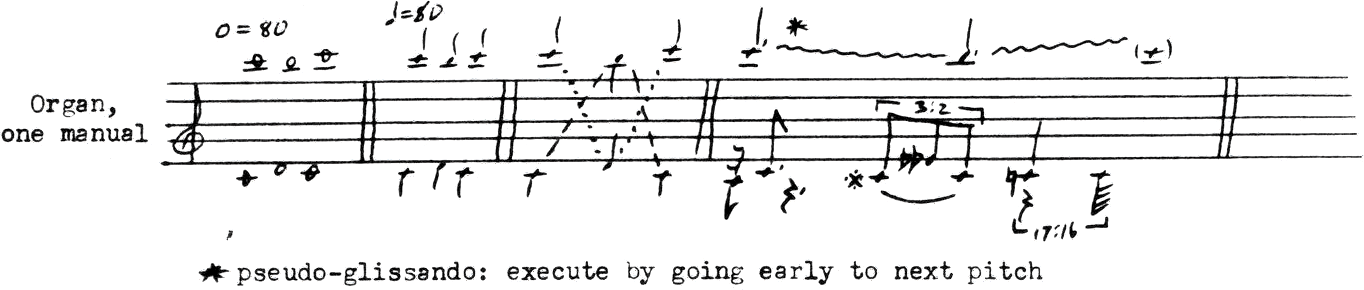
\includegraphics[width=4in]{img/structure_art}\par
}

In each example, the actual sounds, the body of material, is exactly the same. 
The difference is in the different structures defined on the material. The examples 
substantiate my contentions thet the structure is not in the sounds; that the composer's 
analysis of the piece is really a definition and a part of the piece; and that the 
critics' analyses of the structure are definitions attached to the piece, not discoveries 
of intrinsic properties of the sounds. As another example, consider the difference 
between hearing the "Sanctus," \opustitle{Missa Prolationum} of Ockhegem, in no meter (by 
a non-European listener), in one meter (by a lay European listener), and in four 
meters (the intended structure). Arguments such as the one over whether the structure 
of Webern's music is "really" motivic or serial are absurd, since Webern himself did not 
define this point. Many academic structural analyses of art have been irrelevant 
to the aesthetics of the works. 

The purpose throughout all this art is dual; structure or concept art tries to be, 
first, music, visual art, or whatever (which suggests that it is to be listened to, or 
looked at), \emph{and}, something else entirely, to be valuable for its structure or conceptual 
cleverness. Then when the structure is "hidden," "unexperiencable," when it can only be 
appreciated by reading the "analysis," why put emphasis on the body of sound, light, or 
whatever, why listen to structure music, why look at structural visual art, why even call 
them "music," "visual art"? Why not throw away the bodies of sound, light, or whatever, 
and keep the "analyses" of the structure as the works of art? In general, logic, and 
experience (with the results of the artists' efforts), show that the dual purpose of 
structure art consists of irreconcilable objectives; that one can be attained only at the 
other's expense. Which objective are the structure artists trying to attain?---they 
obviously have no idea. Structure art represents obsolete, confused categories of 
activities, categories which by now are obscurantist. Structure (or concept) music, 
for example, needs straightening out, first, by ceasing to call it "music," and starting 
to say thet the sound (or activity) is used only to carry the structure or conceptual 
cleverness, and that the real point is the structure or conceptual cleverness---the 
categorization---and then it will be seen how limited, impoverished the structure of 
these productions trying to be music are. When you make the change, then you are led 
to a far more consistent, integral activity, the same one arrived at below through 
a consideration of pure mathematics. Games of intellectual skill such as chess fall 
into this same category; since, after all, they can be regerded as formalist mathematics. 

Neryt I will discuss pure mathematics. Originally, mathematics was a system of 
beliefs, a doctrine, about the entities numbers, points, polygons, and so forth (Pythagoras, 
Euclid, Platonic geometry). As mathematicians became skeptical, and thus less desirous 
of resting the importance of mathematics on the validity of these beliefs, they changed 
their minds about what the purpose of mathematics is. The purpose became for the theorems 
to be true if the axioms are. In the nineteenth century, as a result of e.g. the ideas 
of Riemann, they became unconcerned to claim that their axioms are true. They began 
to say that the value of mathematics is "aesthetic." Here is when mathematics becomes 
a subject for this essay; when it becomes pure mathematics, when its value is not claimed 
to be that of technology or natural science, but rather more an aesthetic value, when it 
becomes "adoctrinal culture." Mathematics becomes something to be considered alongside art. 
When I became interested in contributing to pure mathematics, for reasons of taste I wanted 
to de-emphasize discovery in mathematics, mathematics as discovering theorems and proofs. 
(Such discovery bored me.) The first way I thought of to de-emphasize discovery was that 
since the value of pure mathematics is now regarded as conceptual interest, aesthetic 
rather than scientific value, why not try to make up aesthetic theorems, without considering 
whether they are true. The second way was to find that the conventional claim that 
theorems and proofs are discovered is unjustifiable; I will return to this point later. 
In the twentieth century, as a result of the ideas of Hilbert, and then Carnap, 
mathematicians became unconcerned to claim that mathematical "statements," the 
mathematical object language, are (substantive) assertions having truth value (as are 
English statements). Rather, they are "merely" series of signs formed according to 
certain rules: formalist mathematics. Then my third way of de-emphasizing discovery was 
to open up unexplored regions of formalist mathematics. The resulting mathematics still 
had statements, theorems, proofs, but the latter weren't "discovered" the way they 
traditionally were. 

Now exploration of the wider possibilities of pure mathematics opened up by me 
tends to lead beyond the form of "making statements," "proving," and the like, so thet 
the term "pure mathematics" becomes completely incongruous. The category of pure 
mathematics---a vestige ultimately of the old system of beliefs canonized by Plato 
(hence the form of statements, proving, and the like)---is an obsolete category. My 
contributions to pure mathematics lead to an integral, general activity of which the 
point is categorizations (having the value of being "well-formed"); the contributions 
need to be classified as such an activity rather than as pure mathematics to escape 
confusion, Traditional mathematics (mathematics as discovery), reformulated, explicated 
to take my findings into account, would be an untypical, small but intensively developed 
part of such an activity. 

The proponents of structure art, pure mathematics, and chess make similar claims 
for them. I have mentioned the claims that structure is an objective property of things; 
and that mathematical theorems and proofs are discovered; and there is a similar claim for 
games of intellectual skill. Two important notions associated with these fundamentally 
identical claims require comment. There is the notion that contribution to structure 
art, pure mathematics, and chess requires high intelligence, the discovery of implications; 
the notion of intelligence as the ability to discover implications. Then, there is the 
notion that structure (as in mathematics pre-eminently) is an objective property of things, 
capable of discovery, demonstration, rational cognition---with particular reference 
to language, art, and the like---whereas meaning, expression, and emotion are not. 
(These pretensions are traditionally an essential aspect of structure art, pure mathematics, 
and chess.) Both notions come down to the belief that there can be an objective relation 
between a name and its referents; for example, an objective relation between the 
metamathematical term "true theorem" and certain theorems, or an objective relation 
between "having serial structure" and a body of sound, or between "checkmate" and 
checkmates. As I said, these notions are discreditable, as can be seen from my 
\essaytitle{Philosophy Proper} and \essaytitle{Primary Paradox}. Thus the notion of intelligence, pretension 
of intellectual superiority, as what mathematicians, chess players, and the like have; 
and the prejudice in favor of structure; cannot be defended. It is about time that 
these notions be discarded. 



\chapter{Exercise Awareness-States (July 1961)}

{
\itshape
The July 1967 issue of IKON contained Henry Flynt's \essaytitle{Mock Risk Games}.
This work was a reconstruction, from memory, of Flynt's 1961 work, 
\essaytitle{Exercise Awareness-States}, which Flynt had disavowed and discarded in 1962. 
In 1981 Flynt obtained a copy of the original 1961 piece in the possession 
of Tom Constanten. In this issue IKON publishes, for the first time, the 
original \essaytitle{Exercise Awareness-States.} Preceding the text, we reprint the 
introduction from \essaytitle{Mock Risk Games} because of its clarity in explaining the 
work. Flynt read \essaytitle{Exercise Awareness-States} during his July 15, 1961 
appearance in the legendary series at George Maciunas' A/G Gallery, NYC. 
This was the only documented public presentation of the work in that period. 
The reconstruction \essaytitle{Mock Risk Games} has been printed a number of 
times --- it was included in Flynt's book, \booktitle{Blueprint For a Higher Civilization}\footnote{That's this!}
(Milan, 1975). 
}


\section*{INTRODUCTION (from "Mock Risk Games"---1967 Version)}


Suppose you stand in front of a swinging door with a nail sticking out of it 
pointing at your face; and suppose you are prepared to jump back if the door 
suddenly opens in your face. You are deliberately taking a risk on the 
assumption that you can protect yourself. Let us call such a situation a "risk 
game." Then a "mock risk game" is a risk game such that the misfortune 
which you risk is contrary to the course of nature, a freak misfortune; and 
thus your preparation to evade it is correspondingly superficial. 

lf the direction of gravity reverses and you fall on the ceiling, that is a freak 
misfortune. If you don't want to risk this misfortune, then you will anchor 
yourself to the floor in some way. But if you stand free so that you can fall, 
and yet try to prepare so that if you do fall, you will fall in such a way that 
you won't be hurt, then that is a mock risk game. If technicians could actually 
effect or simulate gravity reversal in the room, then the risk game would be 
a real one. But I am not concerned with real risk games. I am interested in 
dealing with gravity reversal in an everyday environment, where everything 
tells you it can't possibly happen. Your "preparation" for the fall is thus 
superficial, because you still have the involuntary conviction that it can't 
possibly happen. 

Mock risk games constitute a new area of human behavior, because they 
aren't something people have done before you don't know what they will be 
like until you try them, and it took a very special effort to devise them. They 
have a tremendous advantage over other activities of comparable 
significance, because they can be produced in the privacy of your own room 
without special equipment. Let us explore this new psychological effect; and 
let us not ask what use it has until we are more familiar with it. 

Instructions for a variety of mock risk games follow. (I have played each 
game many times in developing it, to ensure that the experience of playing 
it will be compelling.) For each game, there is a physical action to be 
performed in a physical setting. Then there is a list of freak misfortunes 
which you risk by performing the action, and which you must be prepared 
to evade. The point is not to hallucinate the misfortunes, or even to fear 
them, but rather to be prepared to evade them. First you work with each 
misfortune separately. For example, you walk across a room, prepared to 
react self-protectingly if you are suddenly upside down, resting on the top 
of your head on the floor. In preparing for this risk, you should clear the path 
of objects that might hurt you if you fell on them, you should wear clothes 
suitable for falling, and you should try standing on your head, taking your 
hands off the floor and falling, to get a feeling for how to fall without getting 
hurt. After you have mastered the preparation for each misfortune 
separately, you perform the action prepared to evade the first misfortune and the 
second (but not both at once). You must prepare to determine instantly 
which of the two misfortunes befalls you, and to react appropriately. After 
you have mastered pairs of misfortunes, you go on to triples of misfortunes, 
and so forth. 

\section*{Exercise Awareness-States (July, 1961)}

I am concerned here to introduce an activity which I will call, for want of 
a better term, "exercise," and the states of awareness one has in exercise, 
"exercise awareness-states." Incidentally, this activity is based on wrong, 
although common, philosophical assumptions, but I hope the reader will play 
along with them for the sake of the activity; philosophical rightness is not 
the main concern here. Exercise should be thought of first as training to help 
prepare one for dangerous situations of a very special kind (which the 
reader is admittedly not likely to encounter). (Incidentally, 'danger' here 
should not be an emotive word; my concern is with the theory of defense, 
not with giving the reader vicarious experience.) Suppose that the adults in 
a society occasionally have to be in situations, such as walking across a 
bare metal floor in a certain "building," during which \emph{dangers}, very unusual 
and \emph{unpredictable}, may arise. Suppose that they know nothing of the 
provenance of the dangers, just that they may be there, so that they can't 
prevent them (or predict what they will be); the persons are somewhat like 
animals trying to defend themselves against a variety of modern (human) 
weapons. They cannot adequately prepare for the dangers by practicing 
responses to specific dangers so that they become habitual, because of the 
extreme unpredictability of the actual dangers. However, the dangers are 
such that when one arises a person \emph{can} figure out what he needs to do to 
defend himself \emph{fast enough} and carry it out. 

Finally, suppose that although it is desired to train persons [to be prepared] 
to defend themselves in the situations, there isn't the technology to simulate 
dangers, so that they can't be given a chance to actually figure out and carry 
out defenses against simulated dangers. Then it would seem that the best 
preparation in the situations (until a danger appeared) would be the \emph{state 
of mind}---"unpredictably-dangerous-situation awareness state"---of lack of 
preconceptions as to what one might encounter, emotionlessness (except 
for the small amount of fear and confidence needed to make one maximally 
alert), very very heightened awareness of all sensory data, and readiness 
to figure out (quickly) whether they indicated a danger and [to figure out] a 
defense against it. After all, it might be best to stay away, or at least get 
away, from the preparation resulting from practice with simulated dangers, 
just because the actual ones are so unpredictable. Training for the situations 
would then be to help persons achieve this best dangerous-situation 
awareness-state when in the situations. Then (one should first think) the purpose 
of "exercise," or the "exercises," is to help persons to achieve the best 
dangerous-situation awareness-state in the situations by teaching them to 
achieve "\emph{ultimate} exercise awareness-states," which are as similar as 
possible to the best dangerous-situation states within the limitations I have 
given. 

Exercise may secondly be thought of as something to be done for its own 
sake, so that ultimate exercise awareness-states are achieved for their own 
sake, in particular, as an unusual way of "appreciating" the sensory date 
while in them. This is the way I suppose the reader will regard exercise. Thus 
exercise, rather than unpredictably dangerous situations, is the principal 
subject of this paper. However, it should not be lost sight of that exercise 
could be useful in the first way; and the development of exercises should be 
controlled by concern with whether they are useful in the first way. 

I will now give some explanations and general instructions for exercise. 
An "exercise" is what the general instructions, and a specification of a(n 
exercise) "\emph{situation}" one is to place oneself in and of several 
"\emph{given dangers}" to anticipate in the situation, refers to;
an "\emph{exercise awareness-state}" 
is any state of mind throughout an exercise. In first doing an exercise, one 
anticipates given dangers; the point of having specific dangers to anticipate 
at first is to keep one from anticipating nothing, being indifferent in the 
situation and thus not achieving an interesting awareness-state. In a good 
exercise, the dangers should be interesting to anticipate, one should find it 
easy to anticipate them strongly, and it should be clear what is dangerous 
in them and how they can defended against. It is only when one can 
anticipate the given dangers strongly that one does the exercise, places 
oneself in the situation, without thinking of specific dangers, trying to
strongly anticipate unpredictable danger; when one can do this one will be 
achieving "ultimate exercise awareness-states." 

The general instructions for the exercises follow. First place oneself in the 
situation, anticipate one of the given dangers as strongly as possible (short 
of getting oneself in a state of fright), be very very aware of all sensory data, 
and be ready to figure out (quickly) whether they indicate the danger and to 
start defending against it. Try to achieve the greatest anticipation of and 
readiness for the one danger. The result is an "initial exercise 
awareness-state." Finally one can do the exercise forgetting the given dangers; place 
oneself in the situation, try to anticipate [unpredictable] danger strongly 
(short of getting oneself frightened), without preconceptions as to what form 
it will take, be very very aware of all sense data, and be ready to figure out 
(quickly) whether they indicate a danger, and a defense against it. This is 
an "\emph{ultimate} exercise awareness-state." A final point. So that one will not be 
distracted from the exercise, there must be a minimum of familiar events 
extraneous to it during it, such as the sight of a door opening, talking, 
cooking smells. For this reason, unless otherwise stated exercise should be 
taken in environments as inanimate, quiet, odorless, etc. as possible. One 
will fail to achieve interesting exercise awareness-states if one cannot play 
along and (for the sake of the exercise) strongly anticipate danger; [because 
one doesn't expect it,] but rather remains relaxed, indifferent, or worse is 
sleepy, physiologically depressed (indifferent, depressed exercise states). 
It should be clear that one has to really try the exercises, not just read about 
them, in order to appreciate them. 

\section*{Exercise 1}

The situation: You walk across the floor of a medium-sized brightly lighted 
square room, from the middle of one side to the middle of the other, in a 
straight line. There should be no other animal [fauna, animate creature] in 
the room and the path of walking should be clear [of obstructions]; ideally 
the room should be bare. 

The given dangers to anticipate: 
\begin{enumerate}
\item Heavy invisible objects falling around you, making a whirring noise as 
they do. 
\item Immovability of whichever foot presses most strongly on the floor, and 
a steel cylinder two feet in diameter with sharp edges' falling down, around 
you (hopefully). 
\item Instantaneous inversion of yourself so that you rest on whatever part of 
your surface was uppermost in walking, and doubling of the gravitational 
force on you. 
\item Sudden dizziness, change of equilibrium to that of one who has been 
turning around for a long time, and the floor's vanishing except for a narrow 
strip, where you have walked, shortening from the front. 
\item Change of field of vision to behind your head, instead of in front, 
something's coming to hit you from the side in an erratic path, and loud 
noises on the side of you opposite it. 
\item What you see's suddenly becoming two-dimensional instead of three so 
that you bump into it, while the room fills from behind with a mildly toxic gas; 
and going forward's requiring that you \emph{guess} the unpredictable action, 
symbolic of getting past the barrier, which will enable you to get forward. 
\end{enumerate}

\section*{Exercise 2}

You stand, in a dark room, facing a wall and pulling medium hard with both 
hands on a horizontal bar running along the wall and attached to it, for five 
minutes. Have an alarm clock to let you know when the time is up. There 
should be no other animal in the room; ideally the room should be bare. You 
must not let up on the pulling; the assumption is that if you do your eyes 
and ears will be assaulted with a blinding light and a deafening sound, 
except in the case of certain dangers. 

The dangers: 
\begin{enumerate}
\item Loss of your kinesthetic sense. (body-movement or muscle sense) 
\item Suspension of the "normal" "cause and effect" relationship between 
pulling and keeping the light and sound from appearing, so that you just 
have to guess what to do to keep them from appearing and it changes with 
time, with the restriction that it will be closely related to pulling on the bar, 
\eg\ letting go of the bar. 
\item Suspension of the "normal" "cause and effect" relationship between what 
you will and what your body does, so that you just have to guess what to 
will to keep your arms (and hands) pulling on the bar and it changes with 
time, with the restriction that it will be closely related to willing to pull on 
the bar, \eg willing to let go of the bar. 
\item Having the tactile, cutaneous sensation of being under water, so that 
you will "drown"---"cutaneously"---unless you cutaneously swim to the top; 
your sight and hearing being lost except for sensitivity to the light and sound 
if you stop pulling. 
\end{enumerate}

\section*{Exercise 3}

The situation: You lie on your back, barefoot, on a bunk, your arms more 
or less at your sides, with a pillow on your face so that you can breathe but 
not easily, for five minutes. Do not change your position; the assumption is 
that you can't except in the case of certain dangers. Have an alarm clock 
to let you know when the time is up. The room should be dark and there 
should be no other animal in it. Ideally you should be lying, in the middle 
and along the longitudinal axis of a not uncomfortably hard rectangular 
surface a yard above the floor and having an area almost that of the room, 
in a very long room, which should otherwise be bare. 

The dangers: 
\begin{enumerate}
\item The gravitational force's becoming zero and the room's getting 
unbearably hot towards the ceiling. 
\item Having to press the pillow against your face with your arms and hands, 
except for one angle of your face wherein you can roll your face from under 
the pillow, your head and neck becoming movable. 
\item The surface you are lying on's and the pillow's turning into a two-part 
living organism, of which the lower part is so delicate that unless you 
distribute your bodily pressure on it as evenly as possible, it will be injured 
and the upper part will pull you off of it by the skin of your face in 
self-protection, the organism being sufficiently telepathic that you can 
sense when it is hurting. 
\item Division of your body (and clothing) just below the ribs. The two halves 
separate by 114 feet and a metal wall one inch thick appears between them. 
Matter and so forth are transmitted between halves and they remain in the 
usual position relative to each other so that it is rather as if you simply grew 
in the middle by 112 feet. Your consciousness suddenly seems to be located 
in the pillow, where the pillow is, rather than in your head; nothing that 
happens to the pillow materially affects your consciousness. Two kinds of 
metal blocks come crashing against the wall from far in front of and behind 
it, starting slowly and speeding up as they get near the wall, and then draw 
back to where they came from. Blocks of the first kind come from the front 
(the side the upper part of your body and the pillow are on) only; they are 
"vertical," tall and narrow so that they can be avoided by moving from side 
to side. Blocks of the second kind come in pairs, one in front, one behind. 
They are "horizontal," two feet high (thick), and very wide (long). The ones 
in front hit low and the ones in back high, so they can be avoided by standing 
up (necessarily in a stooped position). Each time the pair hits higher and 
higher. There are long indentations in the back side of the wall in which one 
can get footholds to climb the wall. If one gets to the top of the wall, gets 
both halves of one's body above the wall, they will rejoin. 
\end{enumerate}

\chapter{My New Concept of General Acognitive Culture}

{\itshape [This essay was written c. May 1962 and published in \journaltitle{d\'{e}collage No. 3.} This transcription serves to correct the typographical errors. Footnotes are written in 1992.]}

Of the adult (human) activities I discredit explicitly, consider pure mathematics (and structure art and games of intellectual skill), and Serious Culture\slash all art\slash literary culture\slash science fiction\slash music. I show that these activities (as such) should be repudiated. Now humans are likely in any case to resist this radical idea of repudiating these major institutionalized activities; but especially if nothing were to take their place, if the idea were negative only. Even when the activities' Serious Cultural pretensions have been discredited and repudiated, and their obvious confusions of purpose have been noted,\footnote{cf. \essaytitle{Concept Art} on music} humans are likely to be interested in them still, to like them in at least one respect: for their entertainment, recreational value; for their value as \enquote{ends,} in themselves. (And are thus likely to fear that to repudiate these activities without anything's taking their place would be to give up all recreation, doing things \enquote{just for fun,} doing things just liked.) Now this chapter will be first, an analysis of the concept of entertainment, recreation, of doing things just liked, which will criticize the activities even as just entertainment. (And will discredit my own initial notion of \term{acognitive culture,} as not going far enough.)

I discredit these activities, show they should be repudiated, for \enquote{everybody,} adult humans and creeps. Now since I am a creep, my primary constructive concern is to point out something rather than these activities, for creeps: my new concept of \term{creep acognitive culture.} However, I am going to \enquote{do adult humans a favor} in the hope that it will keep them from just changing the discredited activities into something no less wrong and confused, and will encourage them to repudiate the activities. \enquote{Creep acognitive culture} is, to speak generally, a concept of \enquote{recreation} (resulting from analysis of the concept of recreation) for conscious organisms. Part of it is applicable for adult humans (as well as creeps), in replacing the discredited activities for them. I am going to give that general part here, in this book\footnote{This essay was a chapter in a book in early 1962; that book must have become From Culture to Veramusement.}---my new concept of \term{general acognitive culture.} (The specialization for creeps I will give in Creep.) The specialization of this concept for adult humans I will leave to them, since that is their concern. Incidentally, even though generally applicable, the characteristics of general acognitive culture may be reminiscent of creepiness, but they will not in any case embarrass mature adults, which is where I draw the line between the adult human and the really creep.

To give a better idea of the major area of life, \enquote{recreation,} I am concerned with here, let me mention, along with the activities mentioned above: games, possibly athletics \enquote{for fun,} conventional entertainment and recreation, and children's play. Or \term{acognitive culture} in my initial sense. Further, let me suggest the area with respect to its place in (adult) human life today. Naively, a worker has a job, job hours, an occupation, does work (which produces material wealth), to obtain his means of consumption. His job is a \enquote{means}; even though he may like it he is pretty much forced to do it. This can be extended to apply to the whole area of his responsibilities to society. Then he has after-hours, time when he doesn't have to do anything, and does what he does more as an end, in itself, \enquote{for fun,} because he likes it: here is where recreation is included. This is when workers listen to music, read science fiction, play games, and the rest. A thing is more purely recreational the more it is done just \enquote{for fun,} the more is it is not an extension of the job, a means. This can be extended to apply to the whole area of what he does just because he likes it; and the area can now be conceived as existing (presumably as a matter of course) side-by-side what he does \enquote{for society.} All this can be said about recreation today.

To arrive at the preliminaries of my concept of general acognitive culture, a certain concept of \enquote{recreation} applicable for any conscious organisms (my initial notion of \term{acognitive culture}), let me give some characteristics which the activities I have listed, in their recreational aspect, have in common, which would apply for any conscious organisms. No one of the activities is biologically necessary (or biologically harmful) to the organism. Probably no one is necessary for society, co-operation among the organisms. They are not technology (although they may use it). As (\enquote{mere}) recreation, they are not supposed to have cognitive value (and in particular are without associated cognitive pretensions, so that they cannot be Serious Culture). (They may use believings, especially wrong ones, as \enquote{experiences,} but these are not claimed to have cognitive value in any way.) They do not involve anything, in particular sensuous indulgence, which has sophistication-proving significance. And of course, they are entertainment, recreation, are things just liked. These characteristics are the preliminary, initial determination of the parts of life, of any conscious organism, which I am selecting out to consider as one area, a unity, that of acognitive culture.

Having located and initially determined the area of life I am concerned with, I will now analyze, explicate the concept of pure entertainment, recreation, doing things just liked (with respect to the individual); and at the same time elaborate my new concept of general acognitive culture. Consider, for contrast, work, or the cognitive. With respect to these, there are \enquote{objective} or \enquote{intersubjective standards of value,} for ex., whether a table top is level, or whether many people like a thing. One may well make a contribution to these areas even if one doesn't like the areas, or one's contribution; one can make a level table even if one dislikes the table and finds making it tedious. It makes sense to specially exert oneself to contribute to these areas, to drive oneself to work in them even though one would just as soon do something else. Now 'recreation' connotes, \term{general acognitive culture} is defined to be, exactly the opposite. One does the latter because one likes it (now), for no other reason. It doesn't make sense to try to do acognitive culture as objectively valuable, in conformity with objective standards. If one doesn't like what one does, it can't be acognitive culture. One can't create acognitive culture as a profession.

It is obvious, then, that Serious Cultural institutionalized activities, doing things in Serious Cultural institutional Forms, such as the Fugue, cannot be recreation, acognitive culture. What is not obvious, a point of this analysis, is that the whole institution of society's providing Forms (for the individual to do things in) supposedly for his recreation and self-expression, such as Science Fiction and Pole-Vaulting (or my Linact\footnote{
Linguistic acognitive cultural activity. Extant examples are my \essaytitle{Poem 1} and \essaytitle{Poem 4.}}), is absurd. The notion that the Forms are the real right ones, represent the real right thing to do, are objectively valuable, inevitably grows up around them. As an example, consider the Form of \enquote{Composition,} as any writing of specifications of activities (supposedly) for others to do as recreation. Compositions are primarily the writings, as opposed to doing the activities specified; their existence begins when the writings are completed. They are for \enquote{others} to do (and may never be done by anyone), showing that they are thought to be objectively valuable. The tendency is to turn out and store up quantities of them no matter whether the composer or anyone else likes them. Recreation, acognitive culture, cannot include Composition. Then there is the notion that given a Form, such as I am considering, one should do things in it whether one likes to or not, until one \enquote{understands} the Form, because one will like to then; and that the Form is objectively good if this happens. This has no place in recreation, acognitive culture. People who do things in these Forms all do so largely because they have acquired the notion that the Forms are the real right ones, are objectively more valuable than just anything. A proof of this is that the Forms are so extremely \enquote{objective,} common, impersonal. This is why one can be unable to tell anything about the people themselves from what they do in the Forms. People have no idea of the extreme extent to which they are socialized even in what they do for recreation, self-expression. Even being a writer of any kind, a maker of objects, a creator of works, in the traditional, established, and common sense, is already extremely objective, impersonal, and indicates that one is extremely socialized. (This is what was wrong with my initial notion of \term{acognitive culture}.) The reader may ask, if these Forms are so impersonal, what a personal Form will be like, how personal one can get. The answer will be given below.

Thus, an excellent determining principle is that it's pure recreation, acognitive culture only if it's what one would have done, would do, are doing, \enquote{anyway}; \enquote{prior} (to being \enquote{advanced} enough) to \enquote{know} the real, right, objective, the impersonal things to do, not from trying to contribute to an established real, right Form. Acognitive culture is not created by special exertion. One does it \enquote{anyway} \enquote{first,} and \enquote{then} it turns out to be in the category of \term{acognitive culture.} In fact, the concept of acognitive culture is only used applying retroactively. One doesn't set out to produce so many units of acognitive culture; one realizes that what one did which one would have done anyway was acognitive culture. What, then, is the reason for making the analysis, having the concept at all? Conscientious persons who have suspected the impersonality, of established Forms supposedly for their recreation and self-expression, have had great difficulty in repudiating the Forms, in not being ashamed of not contributing to them, not feeling that they have stopped doing anything. The reason for making the analysis, having the concept, is to help these persons with this difficult step, and to show those who are to give up the discredited activities what replaces them: to show that in giving them up they have not given up doing things just liked. So that they will \enquote{take seriously,} pride themselves on what they do just \enquote{for fun,} doing what they like, would do anyway; rather than being ashamed because they do not contribute to the discredited activities. The analysis, concept, is to make possible an attitude so one can thoroughly, consciously do things just liked.

Since acognitive culture is what one would do anyway, does entirely because one likes it, is for one's liking, it excludes entertaining others, conforming to another's likes---which are an intersubjective standard, making entertaining work. Further, on analysis, being entertained by another, another's creation, becomes questionable. Can the \enquote{creation} of another be liked by oneself, be for one's liking, represent oneself, as well as the \enquote{creation} of oneself? One may admire work by another, with respect to an objective standard, as being better than one's work with respect to that standard, but all that is irrelevant to acognitive culture. If it fits oneself who's doing the liking, if one allows oneself one's likings, then oneself is the source of value and, it would seem, will as a matter of course like one's creations best. Does it make sense for me to appreciate \enquote{great} chess players, poets, pole-vaulters (if their activities are to be regarded as recreation)? My point here is quite radical, but would seem entirely plausible. To go back, analysis of the concept of entertainment shows that separation of entertainer from entertained is incompatible with a thorough-going concept of pure entertainment; entertaining as work is discredited. This does not exclude every kind of involvement of others in one's recreation.

All this leads to the idea of (one's) acognitive culture as a part of oneself---as within oneself, at least so far as specifications are concerned. This would seem to be the opposite of contributions to impersonal Forms. Acognitive culture (being what one would do anyway) would not, it would seem, consist of artifacts built up outside of, separate from, oneself, to be gone back to (for ex. recordings, writings); or specifications one would have to be concerned about remembering. If one is wanting \enquote{what one likes, would do anyway,} one will have it; one shouldn't have to be concerned about retaining it.

The reader may have been asking, 'But may not merely what one would do anyway be less interesting than the pseudo-recreation which is created by special exertion, such as Flynt's \essaytitle{Reproduction of the Memory of an Energy Cube Organism}?' Strictly speaking, this question doesn't make sense: how could anything be more interesting to oneself, likable, than what one just likes, than what one would do anyway \enquote{prior} to \enquote{knowing} the real, right thing to to? However, I will give a heuristic answer to the question. Asking the question shows that one has as yet no idea of what specific doings would be included by the category of \enquote{acognitive culture} as I have defined it. They may well be so different from the discredited activities, the traditional, established, common real right Forms supposedly for recreation and self-expression, as to be irrelevant to them, so to speak. They are going to be indefinitely\footnote{incalculably?} more \enquote{new,} \enquote{different,} interesting, just as individuality is more so than anonymity. It is a matter of one's realizing that what fulfills the supposed function of the discredited activities are things one would not have thought of as replacements for them. All this will become obvious, when one considers what specific doings of oneself meet all of the specifications, are included by the category of \term{acognitive culture} as I have defined it. It may further be asked whether doing just what one would do anyway won't lead to a nihilism of acognitive culture's becoming indistinct, being absorbed in undistinguished personality, life, leaving only \enquote{nature}; or a nihilism that if acognitive culture needs to happen it will just happen, a nihilism of not doing anything. Well, something disappears, namely trying to do things just liked as a real right objectively valuable Form, a profession, by special exertion. However, acognitive culture doesn't disappear, because conscious organisms in any case just do anyway things just liked, which are distinguished, and which are \enquote{then} included by the category of \term{acognitive culture,} \enquote{people have their recreation}---the category of \term{acognitive culture} represents a selecting out of things which presumably the life of any conscious organism will include, for which there will presumably be a place in any life.

As I have mentioned the possibility that the reader may as yet have no idea of what specific doings would be included by the category of acognitive culture as I have defined it, it might seem in order for me to describe some examples of such specific doings. Actually, however, it is just not in the spirit of acognitive culture to try to describe such examples. Real acognitive culture is not likely to lend itself to reduction to words. And trying to describe examples of acognitive culture cannot but be a tendency to make them into works; actually, there is no reason why one's acognitive culture should mean anything to another, or even to oneself at another time. Thus, although I might informally describe examples in conversation, I am not going to try to write any up. The reader who does not yet understand what specific doings are included by the category will just have to study the specifications of acognitive culture some more, and then consider what specific doings meet all of them. When the reader does understand, then he can discover the parts of what he does anyway, already does, that are included by the category of acognitive culture: they are his acognitive culture.

This completes the elaboration of the concept of general acognitive culture. My proposal can now be seen to be plausible, that one give up the discredited activities, all established real right activities which would otherwise be retained as quasi-recreation; and have in their place \enquote{nothing,} except one's acognitive culture, or rather recognition of it. Now this chapter is relatively short, and the ideas in it are intrinsically simple. At the same time, it is of major scope; and it is socially radical, counter to major entrenched interests, institutionalized chess, institutionalized art, Olympic games, and the rest. In the past, there has been a tendency for people to read, but not \enquote{notice,} such writings. I want last to say something to counter any such tendency with respect to this chapter. This chapter may be short and simple, but it is what I have been led to, my complete conclusions, after years of contributing to art and post-artistic activities and thinking about aesthetics and post-aesthetic fields (in an attempt not to waste time as a result of taking the wrong things for granted). Further, it will be outrageous if this chapter is ignored, just bypassed, merely because it discredits major entrenched interests while being short and simple.












\chapter{Primary Study: Informal Paraphrase (1979)}

Consider the assertion that there is (meaningful) language at some time and place---that is, something more than arbitrary marks on paper, something with objective rules and referents. The assertion that there is some language should be a descriptive assertion. (In fact, a descriptive assertion, about natural language, in a natural language.)\footnote{Logical positivists may object that the assertion that there is language is and should be analytic (or meaningless). But this objection cannot be sustained. The attempt to find a criterion which will exclude some grammatical English sentences as meaningless (or analytic) without excluding too many, and without being arbitrary, has always failed. Indeed, is it not so, that one brings out the concepts of "analytic" and "meaningless" arbitrarily, to cover up embarrassing problems? Existence claims, that is, descriptive assertions of the form `There is \uline{\qquad}', are unavoidable in cognition. And it is not plausible that any grammatical natural-language statement is true independently of all experiential or contingent considerations. Nor can an arbitrary, unsubstantiated condemnation of some grammatical statements in the natural language as meaningless be respected. And a retreat to artificial languages cannot evade the questions at issue above.}

The questions at issue here cannot be evaded by retreating to artificial languages, because artificial languages cannot be constructed, or explained, or taught, independently of the natural languages. (Which is why I don't use logical symbols in this study.)

The point is that the assertion that there is language should describe a very definite state of affairs. At birth, every human knows no language at all. For a human to first learn language, language must be related to non-language, or in general, to something outside itself. There is, then, language which is relatable, and related, to non-language. There is some (meaningful) language. There is language. The assertion that our language relates to non-language should be descriptive, just as I said at first.

Since the assertion that our language relates to non-language should be descriptive, it must be possible that it is false. It should be possible to doubt, or even to deny, that there is language, without contradicting oneself or otherwise nullifying oneself (just as it is possible to deny that there is a Taj Mahal without contradicting oneself).

But---

It is not possible to doubt that there is language, or to assert that there never is language, without falling into a fundamental contradiction---because this doubt and this assertion are themselves language.

The assertion that there is language must be true if it can be made at all, unlike a descriptive assertion. The assertion that there is language should be descriptive---but it cannot be.

This "trap" vitiates language. Primary Study (1964) was written to exhibit it, by a more formal approach.

\newcommand\CF[1]{{\centering \vskip 1em \framebox[1.1\width]{\parbox{3.5in}{\vskip 0.5em #1 \vskip 0.5em}} \par \vskip 1em}}

\titleformat{\section}[wrap]{\normalfont\HUGE\filright}{\itshape\HUGE\thesection}{0.5em}{}

\titlespacing{\section}{2em}{2em}{1em}

\titleformat{\subsection}[display]{\scshape\large}{\itshape\thesection}{1em}{}[\titlerule]

\titlespacing{\subsection}{2em}{2em}{1.5em}

\chapter[Communists Must Give Revolutionary Leadership in Culture (1965)][Communists Must Give Revolutionary Leadership in Culture]{Communists Must Give Revolutionary Leadership in Culture (1965)}

\section*{1\hfill}
If the bourgeoisie could keep control indefinitely of the world's most productive 
economies, the U.S. and West Europe, then all cultural leadership, no matter how 
revolutionary, would come to nothing. The culture of the future would be fascist 
barbarism. The discussion of revolutionary cultural leadership is contingent upon 
this state of affairs. 

\section*{2}
\uline{For clarity}, \uline{somewhere}, \uline{sometime}, the \uline{best 
possibility} in culture for the present period has to be defined. As an analogy,
with respect to religion Communists have to state somewhere, sometime that we
are atheists, that the best possibility is the liquidation of religious 
institutions. 

But it is not possible to \uline{implement at once} the best possibility,
before there is a social basis for it. To continue the analogy, a Communist
government cannot have all churches demolished the day it seizes power. Of 
course, when the workers take the initiative, as when the Spanish workers 
burned churches in the Civil War, they must be supported by the leadership
(otherwise it is no leadership). But usually a Communist government must
implement its atheism by guaranteeing \enquote{freedom} of religion; at the same
time closing down the faith healing and religious charity rackets, 
nationalizing church investments, secularizing the schools, teaching atheism,
and in general creating social conditions which tend against escapism among the
masses. Under these conditions atheism should gradually replace religion.

It is the same for culture. A good example is Lenin's directives on the film in
the early years of the Soviet Republic, which were quite advanced. Lenin said to
show the old melodramatic cinemas, yes, to get the people into the movie theatres
and to pay for the his industry; but in the production of Soviet films begin with
socialist documentaries, and require that they appear on every film program along
with the melodramas. 

\section*{3}
The following three conditions for revolutionary cultural leadership are the ones
I will argue from. I will refer to them by letter throughout the text. 
\begin{enumerate}[label=\Alph*., nosep, itemsep=0.5em]
\item To increase the productivity of labor. (For Marxists, a fundamental progressive historical tendency.) 
\item To promote equality and solidarity of the workers; and to tend against the formation of a labor aristocracy, the stratification of the workers by nationality, and the formation of bureaucracies in the proletarian dictatorships. 
\item To satisfy the workers' desire, during a flood tide of class struggle, to come to grips with reality and to be done with escapism in culture. 
\end{enumerate}

\section*{4}
The following is the best possibility in culture for the present 
period. (The many tasks pressing on me allow time only to sketch it.) 
It is important to remember that implementation of the best possibility
by a Communist government can only be in stages. For example, I will say
that the socialist documentary film should replace the filmed melodrama,
\uline{and} that the filmed drama should replace the theatre. In practice this
means to replace the theatre by the filmed drama, while at the same time
to continually increase the proportion of documentaries to theatrical 
films. 


\subsection*{\enquote{Applied Arts}}
These include architecture, automotive products, appliances and
utensils, furniture, graphics, and clothes. Actually, they are nothing
but fields of design engineering which are particularly \uline{retarded} 
by Artistic, national, and stylistic traditions (as well as by the profit
economy). Revolutionary leadership in these fields is to increase the
productivity of labor (Condition A). 

To increase labor productivity in the \enquote{applied arts}, public
ownership is necessary, particularly to escape the forced consumption,
the deliberately wasteful stylisrn required by the capitalist economy;
and a planned economy is necessary, to plan housing and transport as a
whole. But the experience of the Soviet Union shows that these economic
prerequisites do not ensure efficient design. The Soviet Union is 
needlessly backward in the design of automobiles, appliances, furniture,
graphics and clothes. Economic prerequisites and engineering advances
have to be \uline{taken advantage of}: the efficient design has to be chosen 
over the stylized design. 

The oppressed, the poor and illiterate masses as such have nothing to 
contribute to engineering in the \enquote{applied arts}; there can be no 
\enquote{proletarian design}. \enquote{Folk handicrafts}, such as handweaving, pottery,
metalworking must be replaced by mass pro-duction. 

The most efficient architecture, housing today is Soviet prefabricated
concrete architecture. (Appendix 1.) However, this architecture is 
limited by the heaviness of concrete, structural redun-dancy, and 
stylism. Maciunas' prefabricated architecture shows how much farther 
efficiency can be carried. (Appendix 2. A sample of a major material 
in Maciunas' design, expanded polystyrene, is utilized as the back 
cover of this pamphlet.) The Buckminster Fuller geodesic dome is efficient
architecture. (Appendix 3.) 

The Citroen 2CV automobile is efficient, much more so than Soviet 
automobiles. (Appendix 4.) As for clothes, their design is complicated by
their sexual decorative function. However, attractive sports clothes are
often efficient, when they are designed to meet the physical requirements of
the sport. The Soviet decision to copy the freakish Paris fashion industry,
rather than to develop a line of street clothes on the principles of sports
clothes, say exemplifies the reactionary tendency in Soviet \enquote{applied arts}. 

Soviet prefabricated architecture, Maciunas' architecture, the Fuller 
dome, the Citroen 2CV, and this pamphlet show that an efficient artifact
is not a modernistic styled artifact, or even a conventional artifact minus
familiar stylization or decoration. \uline{Efficiency is giving the most performance
for the least cost: to be achieved through complete disregard of 
artistic, national, and stylistic traditions; extensive thought and analysis
in the solution of the design problem; and use of the latest scientific advances.
This principle is completely different, incomparably more advanced and 
intelligent than stylization or decoration; and excludes them.} Efficiency
should replace stylization and decoration. Further, people can be educated to
\uline{like} the achievement of the most performance for the least cost, rather than the more
primitive decoration. 

\subsection*{\textsc{Music (Dancing, \enquote{Poetry})}}

In this area the most oppressed classes and nations have a crucial traditional
culture of their own. For the United States, there are the country blues, 
boogie woogie, R\&B (and Gospel), and the hillbilly music they have influenced.
For Jamaica, there is Blue Beat. For Black Africa, the many tribal musics such
as Baoule and Zulu, either the traditional non-urban varients or the recent 
city-worker variants. For Brazil, macumba music. For India, the analogous music.
For Cuba, bemb\'{e} and as much else as possible from Santer\'{\i}a---if the Government
doesn't wipe it out first. 

In general, for each nation there is a common musical culture which is the
spontaneous creation of those farm-workers and later city-workers who are not
social climbers and can't quit being poor. \emph{Actually, it is usually a fusion of music, dancing, and lyrics---which is done or watched, but not \enquote{performed}. Such a dance of one national grouping comes to another nation not on the Concert Stage, but by people taking it up, doing it.} 
This music-dancing is \uline{already} the indigenous symbols of the oppressed.
In a phrase: \enquote{street-Negro music}. 

To give more examples: For France---during the revolution of 1789, the 
revolutionary masses danced the \uline{carmagnole} in the streets of Paris. Unfortunately,
as a result of the protracted monopoly capitalist stagnation of Europe,
the history of colonialism and the bribing of the workers, there is no native
\enquote{street-Negro music} in France today. The recent ascendancy of an R\&B-inspired
music among British working youth prefigures the path for Europe. 

Street-Negro music cannot be reduced to old or recent European bourgeois Art. 
Nor is it African arts of hundred of years ago which are no longer extant. 
\emph{Further, it must be absolutely clear that street-Negro music is not \enquote{folk art}.}
Street-Negro music is not those \enquote{Negro spirituals} that were \enquote{purified} of 
\enquote{ugly} Africanisms, notated in choral fashion, and performed in the Concert
Hall; or Villa-Lobos'\enquote{Brazilian} Symphonies; or the Kingston Trio; or Odella.
Street-Negro music is not the Russian Moiseyev's Ballets of phony \enquote{folk dances}
performed on the Concert Stage; or the Mexican Ballet Folklorico; or the Cuban
National \enquote{Folk Dance} group; or the Rhumba, \enquote{cleansed} of Africanisrns to become
a ballroom dance. 

Recent trends in street-Negro music prove that it is irreconcilable 
with \enquote{folk art}, that it is hundreds of years \uline{less} antiquated than Bach or 
Mozart, that its modern development is away from European bourgeois Modern 
Art. Such advanced instruments as the many models of electric guitars and 
electric organs (Appendix 5) are standard in R\&B and hillbilly music. Rock'n'roll 
uses such electronic recording techniques as reverberation, dubbing
and over-dubbing. Many numbers are \enquote{studio creations}, exist only in recording.
In addition to the importance of the recording studio in production, there 
is the importance of radio stations in distribution. Street-Negro music rocks;
European bourgeois Modern Art (and \enquote{folk art}) doesn't. 

\enquote{folk art} means something antiquated, humble, and pathetic, and R\&B singer
Buddy Guy's \enquote{First Time I Met the Blues} (Argo LP 4026) comes on too scary for
that put-down. \uline{Bo Diddley} (Chess LP 1431) is good, normal street-Negro music; 
Bo Diddley, use of amplifier reverb and tremolo in \enquote{Pretty Thing} is the 
opposite of \enquote{primitive}. \enquote{Tobacco Road}, by the Nashville musician John D. 
Laudermilk (Columbia Promotion Record 45 RPM 4-41562, JZ SP49232), is the very 
opposite of \enquote{primitive}; and utterly cuts up the \enquote{sophisticated } Nashville Teens'
version. Incidentally, Laudermilk's lyrics are reactionary, but his musical
culture in general is an indigenous symbol of the proletariat. The R\&R which 
jives the snobs and has an electronic sound and is called \enquote{junk music}, such
as \enquote{The Surfin' Bird} by the Trashmen (Garrett Records GA 4002'), is also
by no means \enquote{primitive}. 

For revolutionary leadership, street-Negro music \uline{must be} the 
\uline{point} of \uline{departure. (Condition B.)} Now there is no nonsense about
ringing this music-dancing to the masses, because they created
it. The almost insuperable problem is to bring street-Negro music
to the Communists. Personal aquaintance reveals that \uline{in general}
the instinct of Communists towards street-Negro music is a revulsion
that defies rationality. Communists will say: \enquote{I won't have 
that music in my house.} \enquote{If the Negroes had the opportunity to
hear Fine Music, they would disown that low music.} \enquote{Saxophones
are for playing saxophone \uline{concerti.}} \enquote{Musicians come from 
conservatories.} When people who listen to street-Negro music
become Communists, they sense a hostile and embarrassed reaction 
to the music from their comrades, and they give it up. Communists'
faces are turned \enquote{up} to old European bourgeois Music,
even though they do not know a great deal about it; even though
they cannot analyze the \uline{Grosse Fuge} or a Bruckner Symphony---even
though they have never heard of the insertion syncopations
of \uline{Sumite karissimi}---or of Faugues. Their idea of popular music
is European popular music, Anglo-American music, Mitch Miller 
music. They will fabricate the most tortuous sophistry to prove
that street-Negro music is \enquote{bourgeois corruption}---but that of
course Beethoven's \uline{Solemn Mass in D Major} is not. Communists 
derive self-respect from being too \enquote{high-minded} for those \enquote{vulgar, noisy, trashy} dances. They feel threatened by street-Negro music 
as if it were a bottomless pit of tar. 

But \uline{in general}, the music of the Communists, particularly Anglo-American
popular music, is simply hopeless. It is a cultural expression
of \enquote{white}-chauvinism and racism. It is \enquote{dead} and on
the way out. As I suggested, street-Negro music is already replacing
it among the white masses, wherever they accept rock'n'roll, 
bemb\'{e} or the like. The Communist opposition to this process 
simply will not do. The music of the Communists must be virtually 
replaced by street-Negro music. (Condition B.) 

\CF{The amount that U.S. Communists can do now to implement all this
is of course very limited. But they can do some things. They can be
asked to listen to the R\&B and R\&R radio programs rather than the
other music programs. They can be asked to replace their Classical
record collections. They can be asked to play only \enquote{street-Negro music} at parties. 
We must never sponsor Concerts or, worse yet, 
\enquote{folk} Concerts. If anything, we must sponsor dances. Remember 
that street-Negro music is not a narrow category. lt includes every 
authentic popular music in the world today, except the European
or Anglo-American, which is simply all washed up.}

After the Communists are listening to street-Negro music, then it
will be time to consider that the bourgeoisie \uline{does} manipulate it by
controlling it commercially. In addition to other commercial practices,
the bourgeoisie selects to sell, and encourages, lyrics 
which suit itself---especially in rock 'n' roll. (And the religion in
Gospel, Santer\'{\i}a, and the like is reactionary---but the musical
culture is not, and survives through its influence on secular
music.) Somebody will have to encourage an open call to rebellion
in the lyrics (a step which is irreconcilable with composing cop-out
\enquote{Negro freedom} \enquote{folk songs}).Actually, rebellion is what this
music-dancing is all about; it just couldn't come out under the 
overseer, shotgun or the A\&R man's axe. 

As for \enquote{folk music} and \enquote{folk ballet}, they must be replaced by 
street-Negro music. (Condition B.) All ballet should be replaced 
by this music-dancing. (Condition B. Also, the live Concert Stage
performance is not efficiently produced culture --- Condition A.)
Grand Opera should be replaced by this music-dancing. (Conditions
B, A, C.) All other music should be replaced by it. (Condition B.) 

Even more, Poetry should be replaced by the lyrics of street-Negro
music (Conditions B, C.) 

Revolutionary leadership in music, dancing, "poetry" can only be
as I have stated. No alternative can even be considered. Street-Negro
music is already a vital symbol of the most oppressed; all 
that is needed is encouragement so that it can become more so. 

\subsection*{Film}

Leaving aside the \enquote{applied arts}, the three areas of culture which
have the greatest mass significance are music, the film, and the
novel; and the film tends to become more important than the novel. 

Film-and-sound-track as an area of culture is not engineering;
only the design of the equipment is. However, neither is film
something the oppressed originate. They can originate their own
music by singing while they work; but to realize film-and-track
at all, from camera and recorder to sound projection, requires
time and highly complex equipment. Film is also wholly modern.
It simply hasn't been around long enough to have \enquote{Laws of Art}.
The actual making of films is done exclusively by capitalist or
post-capitalist cultural specialists. It is not the oppressed, but 
intellectuals or cultural specialists who originate film-\enquote{ideas}.
All the poor and illiterate masses as such can do is to respond 
to the films that are shown to them. Thus, there can be no \enquote{proletarian}, 
\enquote{folk} cinema. 

Now \enquote{film} or \enquote{The Cinema} commonly means the \enquote{novelistic cinema},
the \enquote{Theatrical or melodramatic cinema}, the \enquote{acted cinema}. 
That is,the cinema is commonly a photograph of an acted theatrical
drama, staged with sets, actors, costumes, and make-up. In
turn, this drama is usually an adaptation of a fictional-plot novel. 
The Hollywood movie industry is a novelistic cinema industry. The
Russian cinema too, before the Revolution and after Lenin's death, 
is novelistic cinema. 

But during the revolutionary flood tide when Lenin was head of
state, a significant change took place in the Russian film. Lenin
issued a number of directives which said in effect that the novelistic
cinema was merely to be tolerated. Soviet film-makers were 
to concentrate on newsreels and documentaries, and these were 
to be included in every film program. Lenin called for a propagandist 
newsreel series \enquote{From the life of peoples in all countries}.
He expected that these scientific films, as he called them, would 
overcome the influence of the novelistic cinema. (Appendix 6. This
was the only time so far that a Communist politician gave revolutionary 
leadership in culture.) 

At the same time, Dziga Vertov (Denis Arkadyevich Kaufman), a
highly sophisticated cultural specialist who at twenty had been 
in charge of all newsreels of the Russian Civil War, called for the 
virtual replacement of the theatrical cinema by documentaries. He 
made a series of documentaries, using footage of actual events,
and developing new organizations of material to replace the fictional plot. (Appendix 7.)
Vertov's films were popular with the 
Soviet massess, because his films were often the only ones that
showed the new age the people lived in. \uline{Pravda} praised Vertov's
films on its front page. Vertov had the support of celebrities such
as Mayakovsky. Vertov's films even influenced the neo-theatrical
cinemas such as \uline{Strike} and \uline{Potemkin}, unfortunately giving them a 
new lease on life. (When Eisenstein started to make his cinema
\uline{October}, or \uline{Ten Days That Shook the World}, in nine months in
1927, the first three months were taken entirely by the writing of 
the scenario, the fiction, the act. Vertov started by filming the
\uline{events} he wanted to portray.) The first screening of Vertov, \uline{A Sixth
of the Earth} was was for the delegates to the Fifteenth Congress of the
CPSU in 1926, showing the extent of his official acceptance.
Another figure during this high tide of the documentary was Esther 
Shub, who in 1926--7 turned from editing melodramas to make two 
\uline{historical} documentaries from old newsreel footage, \uline{Fall of the
Romanov Dynasty} and \uline{The Great Road} (October anniversary). 

But in the ebb of revolution that followed Lenin, death, the novelistic 
cinematographers again came to the fore, and were supported by Stalin.
Although Vertov continued to be a steadfast opponent
of the novelistic cinema, he abandoned documentaries of
Soviet life for films of primarily technical importance, and portrayals
of Lenin as a Russian deity rather than a political figure.
The novelistic cinematographers won out, and Vertov's work was 
suppressed. From 1937 to his death in 1954, Vertov made no 
more feature films, The feature documentary made a limited come-back
in World War II; but has boon in obscurity ever since. 

Further, Vertov had a serious limitation which put him at a slight disadvantage in his struggle with Eisenstein. None of the Soviet artists were able to stand on their own feet politically; but in addition Vertov was hardly class-conscious at all. Eisenstoin made theatrical, acted cinemas which emphasized the class struggle (fat banker---starving workers); Vertov could have made documentaries which did so even more, but he didn't. Vertov's film reflected Soviet life, but not in a highly class-conscious way. Esther Shub was more political. 

The British cinema is mostly novelistic. But in the early 1930's, during the upsurge of the workers, and under the influence of the Soviet filmmakers l have just discussed, the filmmaker John Grierson and others started the British Documentary Film movement, and the Left adopted the documentary as its own. 

When the documentary has been favored, in Russia, Britain, and elsewhere, the cause has been an upsurge of the workers. I conclude that the predominance of the novelistic cinema, which is like a fantasy or dream, is escapism and false consciousness in a period of reaction. In a period of revolution, real life offers more hope to the oppressed than any fantasy or dream. If the documentary is favored, it is because of the oppressed's desire to conic to grips with reality. Vertov's support of the documentary against the acted cinema, and his techniques, at least, must be the \uline{point of departure} for the revolutionary film-and-sound-track. These documentaries must improve on Vertov, however, by emphasizing the antagonism of the classes. Then, the showing of socialist documentaries must replace the showing of old novelistic cinemas. \uline{(Condition C.)}

The whole production and of course distribution of the film tends toward a high productivity of culture per worker. Vertov himself had a network of cameramen-correspondents throughout the Soviet Union who supplied him with footage. He and his assistants then put it together in his Moscow workshop. Of course, this procedure is standard for the newsreel. 

\CF{
The amount that U.S. Communists can do now to implement all this
is of course very limited. But when our movement is far enough 
along that we have to have cultural activities, we must make our
own films, as the British Left did. They will be documentaries,
making the points specified by the leadership, through the selection
and organization of material. Note that when we publish photographs,
they are always of real events. We never publish photographs 
of scenes staged with actors. Whatever our reason is, it is 
the argument against the novelistic cinema. Further, for us to fool
with the novelistic cinema, with elaborate sets, actors, and cos-tumes
would not only be escapist, but an absurdly wasteful expense.
Then, if the bankers circulate a movie or play so fascist 
that we have to demonstrate against it, we must publicize our own
films in the demonstration.}

\subsection*{\enquote{\textsc{Theatre}}}
The Legitimate Theatre, Broadway and off-Broadway, is a culture of the luxury-consuming \'{e}lite. It is a luxury analogous to handwoven clothes. As soon as Legitimate theatrical productions are a success, they are filmed. The film is far more efficient than the Legitimate Theatre. Even though the Theatre is more original and intimate than the \uline{theatrical} cinema, it will tend to be replaced by films of itself, because of their greater efficiency. The Legitimate Theatre survives to the extent that a luxury-consuming \'{e}lite supports it. 

Vaudeville has reappeared, but on television, on videotape. Even the comic nightclub monologue, which is not being filmed, is being recorded. 

As for the feudal and \enquote{folk} theatres, Noh, the Japanese puppet theatre, the circus, the Brazilian \uline{festa}, they are already dying out, 

Thus, the Legitimate Theatre is a highly inefficient luxury com-pased to the film. It is revolutionary leadership to do everything with the film; to replace the Theatre, including performances of old Dramas, with the socialist film. (\uline{Condition A}: higher labor pro-ductivity; \uline{Condition B}: against \'{e}litist luxuries.) 

\subsection*{\enquote{\textsc{Visual Arts}}}
Before the Invention of photography, much Art involved representation, from Chinese silk painting to the French Academy to Indian sculpture. As photography was developed in bourgeois society in the 19th century, and rapidly achieved widespread popularity, Serious Artists progressively lost Interest In representation. 

The decline of representational Art resulting from the invention of photography is an accomplished fact. The acceptance of this irreversible technical advance is obligatory for revolutionary leadership. (\uline{Condition A.}) As for calligraphy, it is replaced by the Roman alphabet and typography; and as for decoration in the \enquote{applied arts}, I have already dealt with it, 

Bourgeois Artists have turned to producing non-documentational Art Objects, which glorify the bourgeoisie by symbolizing methods. These Art Objects are luxuries, which survive to the extent that a luxury-consuming \'{e}lite supports them. In general, the symbolizing Art Object, and the Art Galleries, are appropriately replaced by the film. \uline{(Conditions B, A, C.)}

It is very significant that during the same high tide of the documentary film I have described: \enquote{At that time the Leftist papers and periodicals carried articles on painting and its expected demise as an art.} The author of those words was Alexander Dovzhenko, a man who had made painting his career, then became so worried by the cultural trend he described that after a sleepless night in his 32nd year, he left his painting studio for good and went into film, 

To conclude, the film's general superiority for culture, in the era in which the masses take over the stage of history, is so great that the theatre and the visual arts must move into its wake. 

The only variety of drawing which symbolizes rather than documents, which the oppressed have shown they want, is the socialist political cartoon. But the political cartoon is an element of journalism; it doesn't have leading cultural significance as does the film. 

\subsection*{\textsc{Fiction}}
The best-seller novel is a \uline{middle-class} art. Its \enquote{equipment}, the ability to read, pen and paper, the prose fictional narrative, is simple. Mass paperback publication and monopolistic distribution of the best-seller make it much more efficient, much less of a luxury then the theatre. However, the film is more immediate, more accessable to the oppressed. 

Many bourgeois intellectuals are becoming more interested in film than in the novel. Even so, the middle classes may continue to demand the best-seller. If they do, the best-seller will present a dilemma. The whole experience of the best-seller shows that it can only have flair, \enquote{freedom}, \enquote{life} when it is irresponsible to the correct political line, to Communist virtuousness. That is, when it is cynical about revolution, scatological, or the like. The novel that approximates the Party line, Marxist historiography, the Socialist Realist novel, can only be stodgy, inept, and dull---and is not a \enquote{best-seller}. There is no getting around it: Dostoevski is more \enquote{alive} than any Soviet novelist; the political cynics, Hemingway, Mailer, Baldwin, and their kind, make the most \enquote{alive} novelists, The reason is precisely that the best-seller violates Condition C. The flair of the best-seller, even the \enquote{true-to-life} best-seller, comes from its fictionality, its fantasy, its escapism, 

No doubt the fiction of Proust, Joyco, Samuel Beckett will die out. (Condition B.) But otherwise there maybe no \enquote{best possibility} for fiction, The politically irresponsible best-seller may have to be permitted indefinitely, if the middle classes demand it. (But not Socialist Realism---we can't back an escapist art that the masses don't even want.)

At best, if the workers' pressure for a revolutionary political line in the best-seller becomes great enough, it may be possible to divert them from the best-seller to the socialist journalistic book and film. (By the \enquote{journalistic book} I mean the book-length account of current events by a writer-participant, such as John Reed's \uline{Ten Days.}) 

\CF{ To implement this, U.S. Communists should encourage filmmakers, not novelists; because we can get so much more out of the film in the short run, as well as the long run. It is wisest for us to leave the writing of the best-sellers to the cynics, who do it so well.}

Can as much established culture as I have said really be exhausted? It is extremely significant that during the same early Soviet period I have referred to, all of the famous cultural specialists, even Eisenstein, even Mayakovsky, believed that Art would ultimately disappear; as every honest history of the period admits. In general, this period was the most revolutionary yet in cultural history; there must be some truth in the unanimous belief of its celebrities, 

\subsection*{\textsc{Theory of Culture}}
Two topics particularly need study. The most important is: Culture as the instrument of an economic class. The overwhelming evidence that culture is a class instrument must be assembled. The other topic is the finances of culture, of the multibillion-dollar cultural institutions: patronage and commissions; Opera boxes; book sales; ticket sales; the Art market; record sales; the banks and the cinema monopolies; the financing of Broadway plays; sponsorship of TV dramas; private endowment of Orchestras, Museums, Concert Halls; state-monopoly capitalist support, which is increasingly important. 

Top published studies of the finances of culture are Francis Haskell's \uline{Patrons and Painters: A Study in the Relations Between Italian Art and Society In the Age of the Baroque}; investment banker Richard H. Rush's \uline{Art As An Investment}; and bourgeois critic Harold Rosenberg's \enquote{The Art Establishment}, in Esquire, January 1965; because they elaborate with Machiavellian frankness on the relation of culture to the ruling class, for a large area of culture. These revealing studies need only be placed in context to have revolutionary implications. Unpublished material of mine which I am collecting under the title \uline{Class and the Development of Culture} will provide an adequate general theory of culture. 

\section*{5}

In many cases a reference to one of Conditions A--C has been a sufficient argument for revolutionary leadership. For example, a reference to Condition A is a sufficient argument for prefabricated architecture. 

Only the applications of Condition B need to be explained: To show that certain \enquote{folk art}, Ballet, Grand Opera, exploiting-class Music (\enquote{Classical} or \enquote{Serious} Music), Poetry, the Legitimate Theatre, bourgeois Modern Art---and European popular music---\uline{promote the formation of a labor aristocracy, the stratification of the workers by nationality, and the formation of bureaucracies in the proletarian dictatorships.}

Economic causes have greatly stratified the world proletariat. The bourgeoisie has used part of the profits from one section of the workers to bribe another section. The low labor productivity of proletarian dictatorships in backward countries is another cause. At the top of the world proletariat is the white labor aristocracy, and the revisionist managers in the proletarian dictatorships; at the bottom are the \enquote{street Negroes}, the \enquote{field Negroes}. The upper layer of the proletariat seeks to consolidate its privileges, and uses methods pioneered by the aristocracies of earlier eras. 

One of the methods pioneered by the aristocracies was through Art. Most of the culture that Condition B excludes originated on commission from exploiters of one kind or another, back when Artists were virtually part of a patrician's stable of servants. The exploiters demanded of their Artists culture virtually prepared to consolidate and enhance the exploiters' position, to differentiate the exploiters as much as possible from the less privileged, the plebeians battering at the doors of privilege. This culture is intentionally wasteful. Where there was national oppression, the culture was prepared to differentiate the exploiters from the oppressed. Today, even though the European bourgeois Modern Artist is no longer a servant, his patrons are the aristocracy of business and finance, The major function of his Art is still to differentiate and consolidate the aristocracy, and the aristocracy of the aristocracy, as Rosenberg's \enquote{The Art Establishment} so brilliantly proves. Yes, this bourgeois critic understands his own class much bettor than the \enquote{Marxist} critics do.

As a consequence, the social climbers, the newly rich and the middle classes, insistently demand Art Appreciation courses to initiate them into the mysteries of snob culture. From this social layer come the \enquote{Marxist} critics, clutching their programs of Music of the Masters, their pamphlets explaining the Old Master Paintings. 

Catholic Music and Art were prepared to awe the serfs, thus consolidating and enhancing the hierarchy's position. They succeeded so well that even the \enquote{Marxist} critics don't recommend then to the workers, A materialist can never agree that the function of Raphael's \uline{Madonnas} was to glorify God. Their major function was to serve their aristocratic patrons. Francis Haskell's \uline{Patrons and Painters} describes both how Italian Baroque painting served the patricians, such as Barberini Pope Urban VIII and Mario de Medici; and how it helped the newly rich, such as Girolamo Manfrin, to climb in society. Then, the whole historical experience of Opera in New York has been that each successive wave of the newly rich, the Astors, Cuttings, Beekmans and Livingstons, then the Vanderbilts, Goulds, Harrimans, Rockefellers and Huntingtons, now the Goldings, Chalks, Grahams (Elizabeth Arden), Lauders, and Cummings', has found Grand Opera---ownership of an Opera Box---indispensable to consolidate its position at the zenith of society. And this consolidation is the historic social function of Grand Opera. Wagner's interest in exclusiveness led him to restrict the performance of his Operas to a specially constructed temple, the \uline{Festspielhaus}; and to encourage his devotees to fast before the performances. Since then his Operas have given unequaled service to the German bourgeoisie. As for the provincial merchants on the make and other lower orders of social climbers, the \uline{Reader's Digest} and Book-of-the-Month Club provide them with their Art Appreciation courses.

Thus, when this culture is introduced among the workers, it promotes their stratification. The labor aristocracy, the revisionist managers, the reactionary intellectuals rally to it. When Art Appreciation is forced on the masses, I am convinced that the most oppressed or class-conscious workers can never embrace the Art in question, the \uline{Turandots} and Bruckner Symphonies, as their own, because it is too alien to their condition. They rightly see it as snobbery. The revolutionary intellectuals, too, instinctively see it as conservative. But it encourages other workers to climb socially, 

Then, snob culture today is dominated by European bourgeois culture, a domination secured by the guns of the imperialists. Its whole \enquote{idea} is that it is high and pure, while street-Negro music is low and \enquote{racial}. This white-supremacist conception will persist as long as snob culture predominates. Snob culture divides the workers into white and black, and consolidates the white workers' position above the black workers. 

An event which illustrates the role of snob culture in the proletarian dictatorships was the appearance of La Scala Opera of Milan at the Bolshoi Theatre in 1964. When it was announced that La Scala would open the 1964--5 Moscow season, the series was sold out almost instantly, Tickets were appropriated by Government Ministries---and their wives' dressmakers. Even the Soviet ticket scalping system (Blat) was helpless as two million requests for seals poured in. La Scala performed \uline{Turandot}, \uline{Trovatore}, \uline{Lucia di Lammermoor}. The first-night audience included almost every member of the Soviet \'{e}lite from Yuri Gagarin to Ulanova. Premier Khrushchev attended the second \uline{Turandot}, and came the next night with his whole family, along with Mikoyan and Marshal Zhukov. On the second night, the 95 brilliant chandeliers of the 134-year-old Bolshoi trembled with the applause from the six tiers of red plush and gold-trimmed balconies. Now the craving of those two million people for tickets, to see (and be seen at) an aristocratic frivolity like \uline{Turandot}, which is precisely what the whole cultural policy of the Soviet Union for decades has been contrived to produce, is a craving to climb into the managerial \'{e}lite. Yes, this culture finds its most appropriate, natural, and indispensable place in the aggressive consolidation of the bureaucracy. It is also significant that the top Soviet performing Artists, Ulanova (the \emph{\enquote{tsarina}} of Dance), Rikhter, Oistrakh, Rostropovich, and the stars of the Moscow Art Theatre, the Ballerinas who after a performance leave the Bolshoi in their fur coats and ride off in their chauffeur-driven private limousines, live in an ease second only to that of the top Government leaders. Sooner or later, the Interpretation of patrician Art requires patrician performers. In People's China too, orchestra players receive twice the salary of steelworkers. 

European popular music is the exception in the culture Condition B excludes, in that it was a revolutionary symbol in 1789. But now that the European and European-American workers have come to have a position in the world proletariat above the colored workers, the \enquote{idea} of European popular music is that it is higher and purer than low, \enquote{racial} street-Negro music. This white-supremacist conception will persist as long as \enquote{white} music does; European popular music now symbolizes white supremacy, Further, the whole idea of \enquote{folk music} and \enquote{folk ballet} is \enquote{cleaned-up n------r music and dances}, European popular music and \enquote{folk music} consolidate white supremacy among the workers. 

\section*{6}
A general remark on implementation of the best possibility for theatre and film. In the early stages of the replacement of the Legitimate Theatre and the novelistic cinema, some more plays and some neo-novelistic cinemas may be produced. These dramas and cinemas present a dilemma exactly analogous to that of the best-seller. They can have "life" only when they are irresponsible to the correct political line. The more they approximate the Party line, the more they will fall flat. LeRoi Jones against the Chinese "proletarian drama": that is the dilemma. The politically irresponsible drama and novelistic cinema may have to be permitted for a while. But a more hopeful possibility is that workers' dissatisfaction with their politics will help to displace them. 

\section*{7}
I have so far limited myself to the present period, but I would like to make one remark with respect to the period after the defeat of the U.S.-European bourgeoisies. Music-dancing will then be an amusement rather than a class-struggle symbol. In the present period, street-Negro music is permeated through and through with \uline{competition}. There is competition between the singers and combos. There is competition on the dance floor. The conceptions of one's superiority to another, one's getting ahead and leaving another behind, or of one's mediocrity or inferiority, are involved. Thus, disappointment and failure are possible in this music-dancing. Now competition is inimical to amusement, I think the people of the future will turn against this competition. They will find a way, in music-dancing and other amusements, for everybody to be "best". 

\section*{{\Large 8}}
If the bourgeoisie could keep control indefinitely of the world's most productive economies, the U.S. and West Europe, then all cultural leadership, no matter how revolutionary, would come to nothing.

% input{extra/philosophy_of_concept_art.tex}

\end{document}
